\documentclass{book}

%%%
% Fichier principal du manuscrit de thèse, à utiliser pour compilation.
%%%

%AUTHOR: Harizo Rajaona
%VERSION: 0.1
%DATE: 2016-01-26

% --- IMPORTS ---

% Pour la mise en page:
\usepackage[a4paper]{geometry}

% Pour les paramètres d'encodage et de langue:
\usepackage[T1]{fontenc}
\usepackage[utf8]{inputenc}
\usepackage[frenchb]{babel}

% Pour les symboles mathématiques:
\usepackage{amsmath}
\usepackage{amsfonts}
\usepackage{mathtools}
\newcommand{\diagentry}[1]{\mathmakebox[1.8em]{#1}}
\newcommand{\xddots}{%
	\raise 4pt \hbox {.}
	\mkern 6mu
	\raise 1pt \hbox {.}
	\mkern 6mu
	\raise -2pt \hbox {.}
}

% Pour améliorer le spacing entre mots, lettres:
%\usepackage{microtype}

% Pour les unités physiques:
\usepackage[load-configurations = abbreviations]{siunitx}
\sisetup{locale = FR,
	detect-all,
}

% Pour mettre du boldface dans les maths:
\usepackage{bm}

% Pour insérer des images:
\usepackage{graphicx}
	\graphicspath{{figures_chap_1/}{figures_chap_2/}{figures_chap_3/}{figures_chap_4/}}
% Pour insérer des images au format eps:
\usepackage{epstopdf}






% Pour l'en-tête et le pied de page:
\usepackage{fancyhdr}
	\pagestyle{fancy}
	\renewcommand{\headrulewidth}{1pt}
	\fancyhead[LE]{}
	\fancyhead[LO]{CHAPITRE \thechapter}
	\fancyhead[C]{}
	\fancyhead[RO]{}
	\fancyhead[RE]{\rightmark}

% Pour mettre une table des matières par chapitre:
% \usepackage[french]{minitoc}

% Pour passer à la ligne si la citation est trop longue:
\usepackage{breakcites}

% Pour régler l'espace inter-ligne dans le texte:
\usepackage{setspace}
	\onehalfspacing

% Pour mettre des hyperliens dans le document:
\usepackage{hyperref}
	\hypersetup{
		colorlinks=true, % colorie les liens
		breaklinks=true, % retour chariot sur liens trop longs
		urlcolor=blue, % couleur des liens
		linkcolor=blue, % couleur des liens internes
		citecolor=brown, % couleur des références
		}
		
% Pour mettre des commentaires/corrections à la relecture:
\usepackage{todonotes}
\newcommand\todoin[2][]{\todo[inline, backgroundcolor=red!20!white, caption={2do}, #1]{
		\begin{minipage}{\textwidth-4pt}#2\end{minipage}}}

% Pour créer une liste des symboles:
\usepackage{nomencl}
	\makenomenclature
	\renewcommand{\nomname}{Liste des symboles}
	
% Pour créer des sous-figures dans un environnement figure commun:
\usepackage{subcaption}


% Pour ajouter les numéros de ligne dans la version draft:
%\usepackage{lineno}
%	\linenumbers
%<<<<<<< HEAD

% Pour écrire des algorithmes en pseudo-code:
\usepackage[ruled, lined, linesnumbered, algochapter]{algorithm2e}
%=======
	
% Pour citer proprement les références:
%\usepackage{natbib}
%	\bibliographystyle{abbrvnat}
%	\setcitestyle{authoryear,open={(},close={)}}
%>>>>>>> corrections_chapitre_1

% --- CUSTOM MATH SYMBOLS ---
\DeclareMathOperator*{\argmin}{\arg\!\min}
\DeclareMathOperator*{\argmax}{\arg\!\max}
\newcommand{\VecTSource}{{\bm{t'_s}}}
\newcommand{\VecPosSource}{{\bm{x_s}}}
\newcommand{\VecQSource}{{\bm{q}}}
\newcommand{\VecObs}{{\bm{\eta}}}
\newcommand{\valObs}{{\eta}}
\newcommand{\VecErreur}{{\bm{\varepsilon}}}
\newcommand{\MatC}{{\bm{C}}}
\newcommand{\MatH}{{\bm{H}}}
\newcommand{\VecTheta}{{\bm{\theta}}}
\newcommand{\VecSigma}{{\bm{\varsigma}}}
\newcommand{\VecSigmaB}{{\bm{\varsigma_b}}}
\newcommand{\CostF}{{\mathcal{J}}}
\newcommand{\MatR}{{\bm{R}}}
\newcommand{\MatB}{{\bm{B}}}
\newcommand{\VecX}{{\bm{x}}}
\newcommand{\PosteriorTheta}{{p(\VecTheta | \VecObs)}}
\newcommand{\MatSigma}{{\bm{\Sigma}}}
\newcommand{\VecThetaCandidat}{{\VecTheta^*}}
\newcommand{\VecThetaCourant}{{\VecTheta^{(i-1)}}}
\newcommand{\VecThetaNouveau}{{\VecTheta^{(i)}}}
\newcommand{\valTheta}{{\theta}}
\newcommand{\VecMu}{{\bm{\mu}}}
\newcommand{\VecPoids}{{\bm{w}}}
\newcommand{\poidsNorm}{{\tilde{w}}}
\newcommand{\VecPoidsNorm}{{\tilde{\bm{w}}}}
\newcommand{\valXMC}{{\upsilon}}
\newcommand{\VecXMC}{{\bm{\upsilon}}}
\newcommand{\kernel}{{\mathcal{K}}}
\newcommand{\corr}{{\rho}}
\newcommand{\propFonc}{{\varphi}}
\newcommand{\ESS}{{\mathbb{ESS}}}
\newcommand{\PosSource}{{\bm{x}_s}}
\newcommand{\obs}{{\eta}}
\newcommand{\PosCapteur}{{\bm{x}_c}}
\newcommand{\varObs}{{\sigma_{obs}^2}}
\newcommand{\stdObs}{{\sigma_{obs}}}
\newcommand{\VecMeanQ}{{\bm{\mu}_q}}
\newcommand{\MatCovQ}{{\bm{\Sigma}_q}}
\newcommand{\MatG}{{\bm{[G]}}}
\newcommand{\MatK}{{\bm{K}}}
\newcommand{\PostMeanQ}{{\widetilde{\VecMeanQ}}}
\newcommand{\PostCovQ}{{\widetilde{\MatCovQ}}}
\newcommand{\varQ}{\sigma_q^2}
\newcommand{\VecThetaMaj}{{\bm{\Theta}}}
\newcommand{\Vecx}{{\bm{x}}}
\newcommand{\Vecv}{{\bm{v}}}
\newcommand{\Vecu}{{\bm{u}}}
\newcommand{\Vecy}{{\bm{y}}}
\newcommand{\Vecmup}{{\bm{\mu}_\varphi}}
\newcommand{\MatSigmap}{{\bm{\Sigma}_\varphi}}
\begin{document}
	\tableofcontents
	
	%\nomenclature[1]{$\mathcal{J}$}{Fonction-coût}
	
	%\printnomenclature
	
	


\chapter{Introduction}

\section{Pourquoi chercher à reconstruire des sources de pollution?}
	La menace de rejets de substances \textit{Nucléaires}, \textit{Radiologiques}, \textit{{Biologiques}} ou \textit{Chimiques} (NRBC) dans l'atmosphère suscite un fort intérêt, du fait des enjeux humains et environnementaux qu'ils affectent. De tels incidents peuvent être d'origine accidentelle, causés par des rejets ayant eu lieu dans des sites industriels stockant ou exploitant des matières dangereuses. Plusieurs événements historiques témoignent de l'impact de tels accidents :\\
	\begin{itemize}
		\item Seveso (Italie) en 1976: un rejet accidentel de dioxine provenant d'une usine chimique engendre un nuage toxique contaminant une surface de près de 2.8 km$^2$, touchant plus de 400 personnes victimes de lésions cutanées, et nécessitant l'abattage de près de 80 000 bêtes contaminées dans les domaines agricoles atteints \cite{Seveso1976}. 
		
		\item Bhopal (Inde) en 1984: une explosion dans une usine de pesticides entraîne un important rejet de substances chimiques toxiques (isocyanathe de méthyle, cyanure hydrogéné) touchant directement la population vivant aux alentours. Le bilan {à} long terme est d'au moins 16 000 morts et d'environ 500 000 intoxiqués \cite{Bhopal1984}.
		
		\item Tchernobyl (Ukraine) en 1986: suite à des erreurs humaines lors d'opérations sur un réacteur de la centrale nucléaire locale, le c\oe{}ur est entré en fusion: il s'en est suivi une explosion et la libération d'importantes quantités d'éléments radioactifs dans l'atmosphère. Le nuage formé par ces polluants s'est répandu à l'échelle continentale sur une grande partie de l'Europe \cite{Repussard2006}.
		
		\item Algésiras (Espagne) en 1998: une usine espagnole incinère accidentellement une source radioactive dans ses hauts-fourneaux. Ce n'est que près de trois semaines plus tard que l'origine de la fuite est établie. Sur la base des mesures effectuées et de la reconstitution des courants atmosphériques, la quantité totale de césium 137 libérée a été évaluée à 1850 GBq \cite{Estevan2003}.
		
		\item Fukushima (Japon) en 2011: suite au déclenchement d'un séisme de magnitude 9.0 au large des côtes japonaises, les dégâts causés par le tsunami induit ont entraîné la fusion d'au moins deux réacteurs de la centrale de Fukushima, causant ainsi d'importants rejets radioactifs sur le territoire japonais, et plus largement, sur une large portion de l'océan Pacifique \cite{IRSN2012}.
		
		\item Igualada (Espagne) en 2015: une citerne explose en effectuant une livraison dans une usine chimique, causant la propagation d'un nuage orange d'acide nitrique. L'incident a entraîné des mesures de confinement des populations dans le voisinage immédiat de l'usine.
		\item Los Angeles (Etats-Unis) en 2015: une fuite localisée dans un puits de stockage de gaz de ville entraîne d'importants rejets de méthane dans l'atmosphère. L'incident a été déclaré le 23 octobre 2015, et annoncé être "sous contrôle" le 11 février 2016 par l'entreprise gestionnaire du puits. Durant la période de rejet, entre 30 et 50 tonnes par heure de méthane furent rejetés dans l'air. Le méthane étant un gaz à effet de serre, les conséquences environnementales à moyen et long terme sont déjà considérées comme graves.\\
	\end{itemize}
	
	Les incidents NRBC peuvent aussi être issus d'actes malveillants relevant du terrorisme. Ce fut le cas à Tokyo (Japon) en 1995, où des membres d'une secte ont percé des poches contenant du gaz sarin (un puissant neurotoxique) dans des rames de métro. Le bilan final {fut}  de 12 morts et plus de 5500 blessés. Plus récemment, le risque d'attentats NRBC a également été mis en évidence  en France suite aux attentats de l'année 2015, et amplifié en raison du contexte géopolitique actuel.\\
	
	Dans tous les cas, il est vital de disposer de techniques rapides pour détecter et évaluer le risque, afin d'assurer au mieux la sécurité des personnes et de coordonner les manoeuvres des équipes de premier secours. De telles techniques reposent sur des méthodes de modélisation des phénomènes physiques régissant l'atmosphère, ainsi que sur un système d'instrumentation permettant, entre autres, de caractériser et quantifier la présence de substances toxiques dans l'air.\\
	
	Cependant, pour que ces outils de modélisation puissent fonctionner, il est indispensable de disposer d'un certain nombre de paramètres, dont les caractéristiques de la source à l'origine du rejet. C'est ce point particulier que nous illustrerons dans la suite de ce chapitre, après un bref exposé introductif sur la physique de la dispersion atmosphérique.\\
	
	\clearpage

	\section{Les principes de la dispersion atmosphérique}
	
	Nous décrivons ici les grandes lignes des règles physiques qui régissent la propagation d'un nuage de polluant dans l'atmosphère. Pour un exposé plus exhaustif, le lecteur peut se référer à \cite{Sportisse2008}.
	
	\subsection{L'équation d'advection-diffusion}
	
	Une fois qu'un polluant est émis dans l'atmosphère, son comportement est régi par plusieurs processus distincts:\\
	\begin{enumerate}
		\item le \textbf{transport}, ou \textbf{advection} qui se fait sous l'influence des circulations d'air dans l'atmosphère,
		\item la \textbf{diffusion}, résultant de la nature turbulente des écoulements dans la partie basse de l'atmosphère (couche limite),
		\item les processus de \textbf{pertes par dépôt sec ou humide}, diminuant la quantité de polluant transportée,
		\item les éventuelles \textbf{transformations physico-chimiques} pouvant altérer l'état du polluant lors de son séjour dans l'atmosphère: la filiation radioactive (s'il s'agit d'un radionucléide), ou les diverses réactions chimiques pouvant avoir lieu avec les autres composants de l'air.\\
	\end{enumerate}
	
	Nous supposerons en première approximation que les processus (3) et (4) énumérés précédemment ne sont pas pris en compte. Si on considère le transport d'un polluant unique dont la concentration peut être décrite au point $\bm{x} = (x,y,z) \in \mathbb{R}^3$ et à l'instant $t$ par une fonction $C(\bm{x},t)$. On peut alors écrire la loi de conservation de la masse pour $C$ sous la forme suivante:
	
	\begin{equation}
	\label{eqn_conservation_masse}
		\dfrac{\partial C}{\partial t} + \nabla \cdot \vec{J}(\bm{x},t) = \VecSigma
	\end{equation}
	où $\VecSigma$ est le \textit{terme source}, $\vec{J}(\bm{x},t)$ représente le flux de masse du polluant, et $\nabla$ désigne l'opérateur gradient. $\vec{J}$ est une fonction vectorielle qui regroupe la somme des phénomènes distincts d'advection et de diffusion: 
	\begin{equation}
	\label{eqn_somme_flux}
	\vec{J} = \vec{J}_A + \vec{J}_D
	\end{equation}
	Le terme $\vec{J}_D$ est associé au phénomène de diffusion. Celui-ci est généralement considéré comme suivant la première loi de Fick, stipulant que le flux de diffusion $\vec{J}_D$ est proportionnel au gradient de concentration : 
	
	\begin{equation}
	\label{eqn_fick_diffusion}
	\vec{J}_D = - \bm{K}\nabla C
	\end{equation}
	où $\bm{K}$ est une matrice contenant les coefficients de diffusion moléculaire, qui dépendent de l'espèce du polluant. Le terme $\vec{J}_A$ est associé au phénomène d'advection, et traduit une dépendance linéaire de la concentration par rapport au champ de vent $\bm{\vec{u}}$:
	
	\begin{equation}
	\label{eqn_flux_advection}
	\vec{J}_A = C\bm{\vec{u}}
	\end{equation}
	La combinaison des équations \eqref{eqn_somme_flux}, \eqref{eqn_fick_diffusion} et \eqref{eqn_flux_advection} mène ainsi à la formulation de l'\textit{équation d'advection-diffusion}, formulée sur le modèle de \cite{Stockie2011}:\\
	
	\begin{equation}
		\label{eqn_advection_diffusion}
		\dfrac{\partial C}{\partial t} + \nabla \cdot(C\bm{\vec{u}}) = \nabla \cdot (\bm{K}\nabla C) + \VecSigma
	\end{equation}
	Cette équation constitue la base de départ pour les différents modèles numériques cherchant à simuler les phénomènes de dispersion atmosphérique.\\
	
	\subsection{Les différents modèles de dispersion}
	
	Suivant les situations, la taille du domaine sur lequel les calculs sont effectués peut grandement différer. On distingue habituellement : \\
	\begin{itemize}
		\item l'\textit{échelle locale}, aussi appelée \textit{micro-échelle} (jusqu'à 1 km): à ce niveau, des phénomènes spécifiques tels que la présence de bâtiments doivent être pris en compte dans le calcul des champs de vent. C'est à cette échelle qu'il convient de se placer pour traiter les études d'impact en milieu urbain (par exemple à l'échelle d'un quartier), ou sur un site industriel. 
		\item la \textit{méso-échelle}, ou \textit{échelle régionale} (jusqu'à 1000 km): elle est utilisée pour travailler sur des phénomènes plus larges, par exemple pour étudier l'impact de la pollution à l'ozone ou aux particules fines sur le territoire d'un pays tel que la France. 
		\item l'\textit{échelle planétaire}, ou \textit{échelle synoptique} ($>$ 1000 km): on s'intéresse ici à l'impact d'événements de très grande ampleur, tels que les {accidents} de Tchernobyl ou Fukushima. \\
		
	\end{itemize}
	
	On peut également noter la corrélation entre les échelles spatiales et temporelles dans le cadre accidentel: au niveau local, on s'intéresse typiquement à des phénomènes n'excédant pas quelques heures, alors qu'à l'échelle du globe on se place sur un intervalle de plusieurs semaines, voire plusieurs mois.\\ 
	
	Pour couvrir efficacement ces différentes tailles de zones, plusieurs types de modèles de dispersion existent. Ceux-ci se divisent en quatre catégories principales:\\
	
	\begin{itemize} 
		
	\item \textbf{Les modèles gaussiens}:
	Sous certaines hypothèses simplificatrices, l'équation \eqref{eqn_advection_diffusion} peut donner des solutions analytiques pour déterminer la concentration de polluant au sein de \textit{panaches} ou de \textit{bouffées} selon la configuration choisie. \cite{Stockie2011} résume les principes régissant les modèles gaussiens, et une présentation plus détaillée de leur fonctionnement sera introduite au Chapitre 3 du présent manuscrit.\\
	
	\item \textbf{Les modèles eulériens}:
	Le domaine de simulation sur lequel est résolue l'équation \eqref{eqn_advection_diffusion} est discrétisé en un maillage de calcul  par des méthodes numériques. On retrouve ce type d'approche dans des études de cas à l'échelle continentale \cite{Saunier2013} ou globale. \\
	
	\item \textbf{Les modèles lagrangiens particulaires}:
	Dans le cadre lagrangien, le rejet est modélisé comme un ensemble de particules numériques porteuses d'une masse élémentaire. Le modèle suit la trajectoire de chaque particule, dont le mouvement moyen est constitué d'une composante régie par le champ de vent, et d'une composante stochastique traduisant la variabilité causée par la turbulence. La concentration mesurée sur un volume élémentaire du domaine à un temps donné est ainsi égale à la somme des masses élémentaires portées par chaque particule contenue dans ce volume à cet instant. Ce type de modèle est présenté plus en détails au Chapitre 4.\\
	
	\item \textbf{Les modèles de mécanique des fluides}:
	Aussi appelés \textit{Computational Fluid Dynamics} (CFD), ces modèles sont utilisés à petite échelle, et impliquent une résolution des équations de Navier-Stokes sur un maillage relativement fin. Il en résulte une {très} bonne précision des calculs, en particulier en cas de présence d'obstacles menant à des écoulements complexes.\\
	
	\end{itemize}
	
	
	\section{Les caractéristiques du terme source}
	
	Les modèles de dispersion présentés dans le paragraphe précédent nécessitent plusieurs types de données d'entrée: 
	\begin{itemize}
		\item un certain nombre de \textbf{paramètres météorologiques}: dans le cas le plus simple, on considère la direction et la vitesse du vent mesurés par une station au sol dans le domaine d'étude ou à sa proximité, ainsi que la stratification atmosphérique. Ces données sont alors supposées homogènes. Dans des cas plus complexes, plusieurs instruments météorologiques peuvent être pris en compte, au sol comme en altitude. Enfin, il est également possible d'exploiter les résultats d'un système de prévision météorologique: les grandeurs considérées sont alors des champs de vitesse et direction de vent, température, humidité, nébulosité et flux de rayonnement.
		\item les \textbf{paramètres de la source} à l'origine des émissions à modéliser{;}
	\end{itemize}
	
	C'est sur ce second point que nous allons plus particulièrement nous pencher dans la suite de ce paragraphe. En effet, la terminologie employée pour décrire la source d'un rejet polluant peut parfois prêter à confusion, car il existe plusieurs façons d'en décrire les caractéristiques. Nous fixons ici les termes utilisés pour distinguer les différents types de source rencontrés.\\
	
	Une source est dite \textit{localisée} si sa position peut être réduite à un point de l'espace, on peut également parler de \textit{source ponctuelle}. Par opposition, une \textit{source étendue} est caractérisée par une surface d'émission, il peut, par exemple, s'agir d'un bac de décantation dans une usine de retraitement des déchets, si on se place à une échelle suffisamment petite.\\
	
	Une source est également définie par le profil temporel de son rejet, autrement dit la variation de la quantité de polluant rejetée par unité de temps. Comme nous travaillons dans un cadre de modélisation numérique d'un phénomène physique, il est nécessaire de définir une discrétisation temporelle sur $T_s$ instants d'émission, sous la forme d'un vecteur $\bm{t'}_s = (t'_1, \dots, t'_{T_s})$. On peut alors construire le vecteur du profil d'émission comme étant la liste des quantités rejetées par pas de temps d'émission (figure \ref{fig_courbe_profil_source}) : 
	
	$$ \VecQSource = \left(q(t'_1), q(t'_2), \dots, q(t'_{T_s})\right)$$
	
	Si le rejet est suffisamment bref pour n'être effectif que sur un unique pas de temps, alors $\VecTSource$ est réduit à un scalaire $t'_s$, et $\VecQSource$ à une masse totale émise $q_s$ : dans ce cas, on parle d'une source dite \textit{instantanée}. Dans le cas inverse, et lorsque le débit n'est pas constant, on parle d'une source \textit{non-instantanée}. Si $ \forall i \in \{1, \dots, T_s\}, ~ q(t'_i)$ est constant, la source est dite \textit{continue}. \\
	
	
	\begin{figure}[hb]
		\centering
		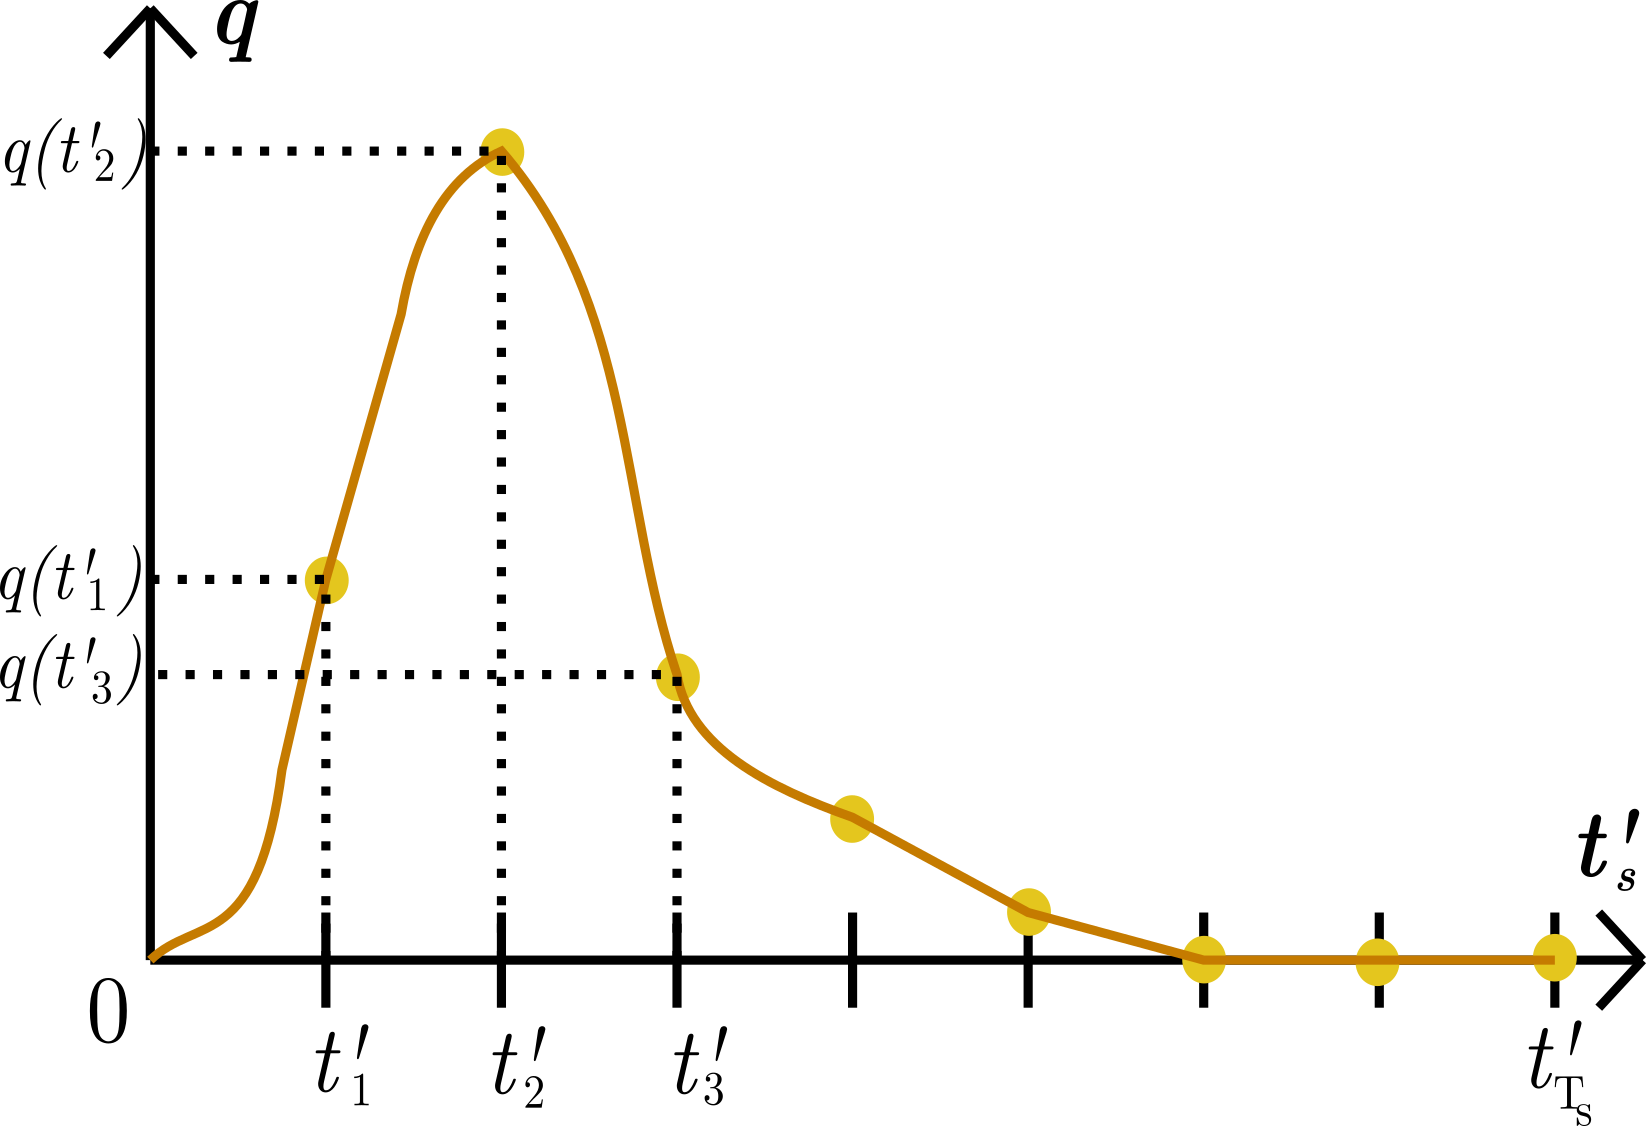
\includegraphics[scale=0.6]{courbe_profil_source.png}
		\caption{Exemple de discrétisation d'une source non-instantanée.}
		\label{fig_courbe_profil_source}
	\end{figure}
	
	Enfin, un cas d'étude peut comporter une \textit{source unique}, ou bien avoir une configuration \textit{multi-sources}.\\
	
	%
%	\subsection{Paramétrisation et relation source-récepteur}
%	

%	
%	
%	\begin{equation}
%		\label{eq_relation_SR_non_parametrique}
%		\VecObs = \bm{H}\VecSigma + \bm{\varepsilon}
%	\end{equation}
%	

%	
%	Dans le cas particulier d'une source ponctuelle on peut, dans l'équation \eqref{eq_relation_SR_non_parametrique}, substituer $\VecSigma$ par un profil d'émission $\VecSigma$ issu d'un unique point du domaine spatial considéré. En procédant ainsi, il n'est plus nécessaire de définir arbitrairement un maillage conditionné par $N_x, N_y, N_z$  sur le domaine. De plus, la dimension du problème se réduit à estimer un point de l'espace et son profil temporel associé, soit $T_s + 3$ inconnues, contrairement au cas général où il faut retrouver l'intégralité du champ d'émission, soit $N_xN_yN_zT_s$ inconnues.\\
%	
%		
\todoin{ ---------- NOUVEL ETAT DE L'ART ----------}
	\section{Estimation du terme source: un état de l'art}
	\label{section_etat_art_STE}
	
	\subsection{Une brève introduction aux problèmes inverses}
	Le domaine des problèmes inverses constitue un vaste champ de la littérature scientifique, et de nombreux travaux y ont été menés. En pratique, résoudre un problème inverse revient à reconstituer un signal, une image, ou plus généralement une donnée non-observable à partir de mesures existantes, appelées observations.
	Cette approche est duale à celle du problème direct où, à partir d'un signal ou d'un ensemble de paramètres initiaux, on cherche à en calculer les effets après une transformation donnée (figure \ref{fig_diagramme_direct_inverse}).
	De nombreux domaines théoriques et pratiques font appel aux méthodes inverses. Le lecteur pourra trouver une revue complète de ces applications dans \cite{Tarantola2004}, on peut en citer quelques exemples tels que la géophysique \cite{Backus1967}, l'acoustique \cite{Kirsch1988}, l'imagerie satellite \cite{Park2003} et médicale \cite{Arridge1999}, les transferts thermiques \cite{McCormik1992} ou encore la finance quantitative \cite{Dembo1999}.\\
	
	\begin{figure}
		\centering
		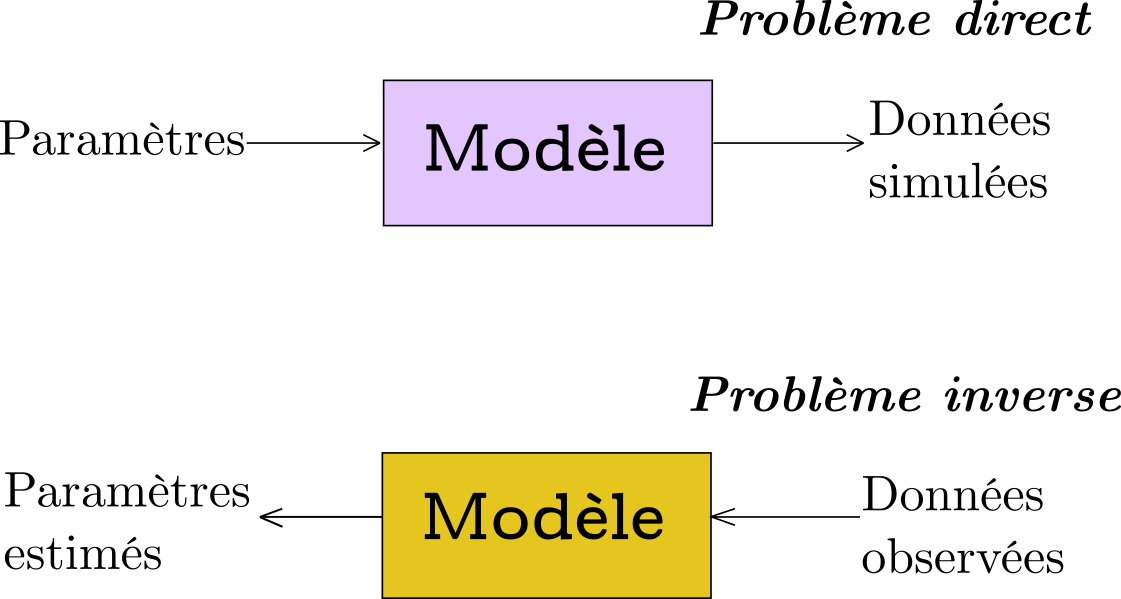
\includegraphics[scale=0.5]{diagramme_direct_inverse.png}
		\caption{Schéma de principe illustrant la dualité entre problèmes direct et inverse.}
		\label{fig_diagramme_direct_inverse}
	\end{figure}
	
	
	En dispersion atmosphérique, le problème direct peut ainsi se traduire par la donnée des paramètres de la source au modèle de dispersion, qui va produire le champ de concentration résultant. Cela revient bien à définir le problème inverse comme étant la reconstruction des paramètres de la source à partir des mesures de concentrations aux capteurs. Nous décrivons dans les paragraphes suivants les différentes approches existantes dans la littérature permettant de résoudre ce problème. Des éléments complémentaires sur la question sont également disponibles dans \cite{Rao2007}. Dans un souci de brièveté, par la suite nous qualifierons de "problèmes STE" (\textit{source term estimation}) toutes les études de cas visant à estimer les paramètres d'une ou de plusieurs sources inconnues.\\
	
	
 \subsection{Backtracking et modèles adjoints}
 
 Une première possibilité consiste à étudier le problème dual associé à l'équation d'advection-diffusion  \eqref{eqn_advection_diffusion}, en inversant la flèche du temps, et par conséquent la direction du vent.  Par le principe de symétrie présenté dans \cite{Hourdin2006a}, on peut alors introduire la notion de \textit{rétro-transport} ou \textit{backtracking} en  réécrivant l'équation d'advection-diffusion sous la forme : 
 
 \begin{equation}
 \label{eqn_advection_diffusion_backward}
 \dfrac{-\partial C^*}{\partial t} - \nabla \cdot(C^*\bm{\vec{u}}) = \nabla \cdot (\bm{K}\nabla C^*) + \VecObs
 \end{equation}
 
 où $C^*$ est un champ de concentrations conjuguées, ou \textit{rétro-concentrations}, dont les valeurs sont obtenues par des rétro-rejets virtuels depuis les capteurs vers la source. Le modèle de dispersion associé à cette démarche duale est alors appelé \textit{modèle adjoint}, ou \textit{modèle backward}. Cette démarche revient ainsi à transformer le champ d'émission de \eqref{eq_relation_SR_non_parametrique} en un champ de rétro-émissions issues des capteurs, comme illustré sur les figures \ref{schema_probleme_direct} et \ref{schema_probleme_inverse}, et ainsi fournir une estimation qualitative du terme source.\\
 
 \begin{figure}[h]
 	\begin{subfigure}{0.5\textwidth}
 		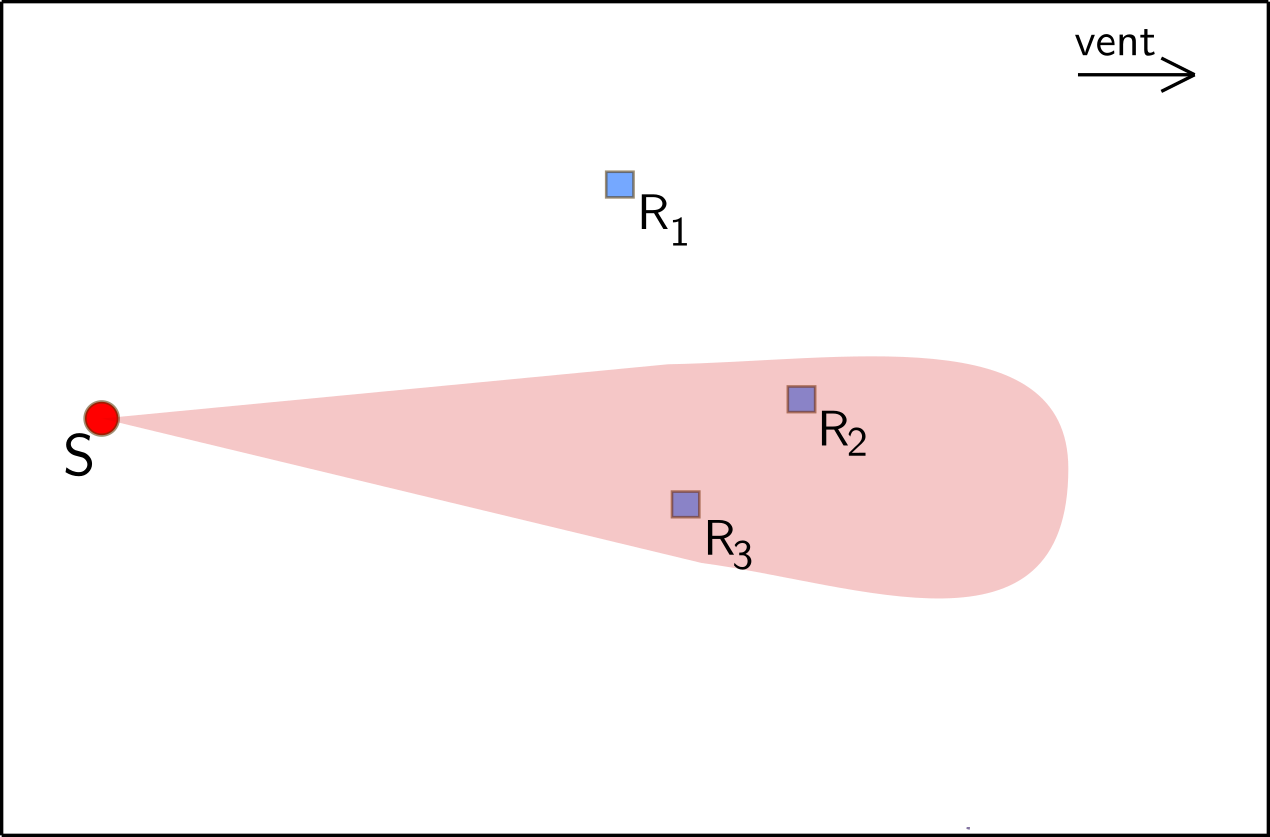
\includegraphics[scale=0.6]{schema_probleme_direct.png}
 		\caption{Approche orientée source}
 		\label{schema_probleme_direct}
 	\end{subfigure}
 	\begin{subfigure}{0.5\textwidth}
 		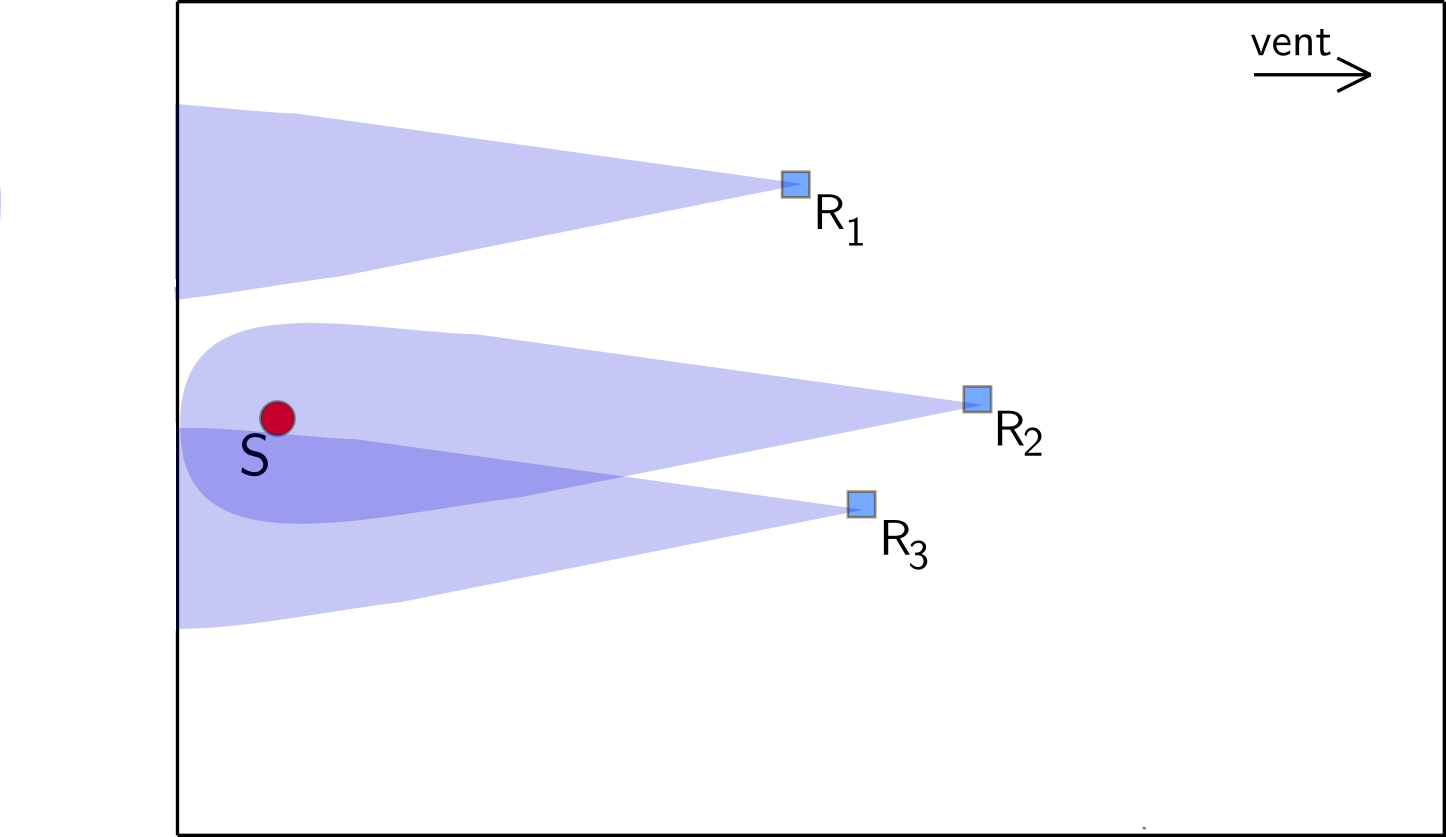
\includegraphics[scale=0.2]{schema_probleme_inverse.png}
 		\caption{Approche orientée récepteur}
 		\label{schema_probleme_inverse}
 	\end{subfigure}
 	\caption{Exemple illustrant la relation entre une source unique $S$ et trois capteurs $R_1,R_2,R_3$ sur un problème en deux dimensions pour les approches en "direct" (\ref{schema_probleme_direct}) et en "adjoint" (\ref{schema_probleme_inverse}). }
 \end{figure}
 
 Dans \cite{Flesch1995}, un modèle \textit{backward} lagrangien est construit pour estimer le profil de rejet d'une source surfacique.  Cette méthode est également appliquée dans \cite{Pudykiewicz1998}, où la position et l'intensité du terme source de Tchernobyl sont reconstruits. De même, dans \cite{Hourdin2006b} le principe du \textit{backtracking} est appliqué à un modèle eulérien pour retrouver la source de la campagne ETEX\footnote{L’expérience \textit{European Tracer EXperiment} (ETEX), menée en 1997,  a consisté à mesurer et étudier l'impact à l'échelle européenne de rejets de gaz traceurs passifs émis depuis le nord de la France \cite{Nodop1998}.}.\\
 
 \subsection{Formulation linéaire du problème et optimisation}
 \label{subsection_MCO}
 
Le modèle direct de simulation des concentrations résultant d'un rejet de polluant peut être décrit de façon linéaire. Pour cela, on définit de façon arbitraire un maillage dans le temps et l'espace qui couvre respectivement la période d'observation et le domaine spatial considérés. En pratique, cela revient à discrétiser l'espace en $N_xN_yN_z$ points, chaque point étant associé à un profil d'émission de longueur $T_s$. Dans un tel contexte, le terme source est défini comme un vecteur $\VecSigma \in \mathbb{R}^{N_\VecSigma}$ (où $N_\VecSigma = N_xN_yN_zT_s$).Il est ainsi possible de lier les observations générées par le modèle et le vecteur source $\VecSigma$ par la formule suivante, appelée \textit{relation source-récepteur}:

\begin{equation}
	\label{eq_relation_SR_non_parametrique}
	\VecObs = \bm{H}\VecSigma + \bm{\varepsilon}
\end{equation}
où $\VecObs \in \mathbb{R}^m$ représente le vecteur des observations, $\VecSigma \in \mathbb{R}^{N_\VecSigma}$ la source discrétisée et $\bm{H} \in \mathbb{R}^{m \times N_\VecSigma}$  la \textit{matrice de transfert}. Le rôle de $\bm{H}$ est d'assurer la projection depuis l'espace $\mathbb{R}^{N_\VecSigma}$  de la source vers l'espace $\mathbb{R}^m$ des observations grâce à l'utilisation d'un modèle de dispersion atmosphérique. $\bm{\varepsilon} \in \mathbb{R}^m$ est le vecteur des erreurs d'observation, et prend en compte les erreurs de mesure, de représentativité et de modèle. \\

Retrouver le terme $\VecSigma$ dans l'équation \eqref{eq_relation_SR_non_parametrique} revient alors à résoudre un problème inverse linéaire: il existe pour cela différentes méthodes que nous détaillons ci-après.

\subsubsection{Définition de la fonction-coût à optimiser}

L'équation \eqref{eq_relation_SR_non_parametrique} peut être réécrite sous la forme : 
 
 \begin{equation}
 \VecObs = \widehat{\VecObs} + \VecErreur
 \label{eq_relation_SR_nonparam_simple}
 \end{equation}

où $\widehat{\VecObs} = \MatH \VecSigma$ est l'approximation des observations $\VecObs$ par le processus de modélisation. On voit bien que dans le cas parfait où ce dernier reproduit exactement les observations attendues, on a $\VecErreur = 0$ et par suite $\widehat{\VecObs} = \VecObs$. Le fait de chercher la valeur $\VecSigma$ pour laquelle $\widehat{\VecObs}$ se rapproche le plus de $\VecObs$ permet ainsi de définir le problème STE sous la forme d'une minimisation de l'erreur $\VecErreur$: on définit pour cela une fonction-coût qui s'écrit : 

\begin{equation}
\CostF(\VecSigma) = ||\VecObs - \MatH \VecSigma||_p = ||\VecObs- \widehat{\VecObs}||_p
\label{eq_cost_function_definition}
\end{equation}
où $||\cdot||_p$ désigne une norme $L_p$ arbitrairement choisie. La résolution du problème STE se traduit alors par la minimisation de cette fonction-coût:

\begin{equation}
\widehat{\VecSigma} = \argmin_\VecSigma \mathcal{J}(\VecSigma)
\label{eq_argmin_cost_function}
\end{equation}
où $\widehat{\VecSigma}$ est l'estimation du terme source recherchée.

\subsubsection{Minimisation d'une fonction-coût quadratique}

Une des approches les plus courantes pour résoudre l'équation \eqref{eq_argmin_cost_function} consiste à choisir $p=2$, autrement dit à minimiser l'écart quadratique entre les observations $\VecObs$ et les données générées par le modèle direct. Concrètement, cela revient à optimiser la fonction-coût suivante:

\begin{equation}
\CostF_{2}(\VecSigma) = ||\VecObs - \MatH \VecSigma ||_2^2
\label{eq_cost_MCO}
\end{equation}

Le fait de minimiser $\CostF_2$ revient à appliquer la méthode des \textit{moindres carrés} pour résoudre le problème inverse. 

Le terme d'erreur que nous cherchons à minimiser est une combinaison des différentes sources d'incertitudes existantes (mesure, représentativité, modèle). Comme il est difficile de quantifier les contributions respectives de ces dernières, on peut invoquer le principe du maximum d'entropie pour définir la représentation statistique de l'ensemble des incertitudes comme étant un bruit gaussien centré et de matrice de covariance $\MatR$ : 
\begin{equation}
\VecErreur \sim \mathcal{N}(0,\MatR)
\label{eq_bruit_obs}
\end{equation}

Dans le cadre de statistiques gaussiennes, la fonction-coût peut alors s'écrire sous la forme suivante \cite{Winiarek2011}:

\begin{equation}
\mathcal{J}_2(\VecSigma) = \dfrac{1}{2}(\VecObs - \MatH \VecSigma)^T \MatR^{-1}(\VecObs - \MatH\VecSigma)
\label{eq_cost_forme2}
\end{equation}

Plusieurs travaux dans la littérature ont recours a cette formulation: \\
\begin{itemize}
	\item Dans \cite{Kathirgamanathan2002}, un point source instantané est estimé à l'aide d'une méthode des moindres carrés, cette source étant caractérisée par sa masse totale émise, sa position et son instant d'émission. L'étude qui y est menée met notamment l'accent sur l'influence du dimensionnement du réseau de capteurs sur la performance de la reconstruction : au moins trois points de mesure sont nécessaires, et la distance entre les différents capteurs influe sur la qualité de l'estimation.\\
	
	\item Dans \cite{Ryall2001}, ce sont des zones d'émission plus grandes qui sont estimées pour des rejets de gaz à effet de serre sur plusieurs années. \\
	
	\item Dans \cite{Matthes2005}, une approche en deux temps est formulée afin de résoudre un problème de complexité proportionnellement croissante au nombre de capteurs. Dans une première étape, les mesures individuelles de chaque capteur produisent des ensembles de positions probables pour la source. Dans un deuxième temps, ces ensembles sont comparés pour estimer la meilleure position en faisant varier l'intensité de la source à retrouver. \\
	
	\item  Dans \cite{Robertson1998}, l'inversion est faite dans le cadre de l'assimilation de données: cette méthodologie permet de corriger de façon variationnelle les paramètres du modèle de dispersion selon une boucle de rétro-action basée sur des observations. Très utilisée en météorologie, l'assimilation de données agit en deux temps selon un principe de "prévision-correction", et itère sur le cycle suivant:
	\begin{enumerate}
		\item  on calcule d'abord une ébauche de l'état à l'instant présent $t$, en appliquant un modèle de prévision en $t-1$,
		\item  on exploite ensuite les observations disponibles à l'instant $t$ pour corriger les paramètres du modèle en les comparant avec l'ébauche. \\
	\end{enumerate}
	
	 \item \cite{Issartel2005} mentionne le principe d'\textit{illumination}, qui est une mesure quantitative de la représentativité des mesures dans le temps et l'espace. Dans le cadre d'un modèle adjoint, l'illumination permet ainsi de caractériser des zones qui ne sont pas forcément couvertes par les rétro-émissions issues des capteurs, par exemple si la zone considérée est relativement éloignée du point de mesure le plus proche. Cependant, si l'information d'illumination est utilisée pour inverser un terme source, alors elle aura tendance à fortement favoriser les solutions proches des capteurs. Pour compenser ce problème, une phase de \textit{renormalisation} est introduite (\cite{Issartel2007} et \cite{Sharan2009}) pour équilibrer l'information apportée par chacun des capteurs. D'abord utilisée à grande échelle, cette méthodologie a récemment été validée à l'échelle locale dans \cite{Singh2014}, et dans un contexte urbain par \cite{Kumar2015}. \\

\end{itemize}

\subsubsection{Régularisations}

Bien souvent, le nombre d'observations à notre disposition est limité, à cause par exemple d'un faible nombre de capteurs ou d'une mauvaise représentativité temporelle dans les mesures fournies par ces derniers. Dans de telles situations, le problème inverse peut admettre une infinité de solutions, et ainsi devenir \textit{mal-posé}. Rappelons qu'un problème \textit{bien posé} au sens de Hadamard \cite{Hadamard1902} désigne un modèle mathématique dont la solution existe, est unique, et dépend de façon continue des données. A l'inverse, un problème mal-posé déroge à au moins une des règles précédemment citées. \\

De nombreux problèmes physiques sont intrinsèquement mal-posés, et des solutions existent pour les \textit{régulariser}, c'est-à-dire leur appliquer une transformation qui permet de revenir à un problème bien posé. Parmi ces méthodes, la \textit{régularisation de Tikhonov} \cite{Tikhonov1963} est la plus fréquemment employée: elle consiste à ajouter un terme $\lambda_B ||\VecSigmaB||_2$ dit \textit{régularisant} à l'expression de la fonction-coût $\CostF_2$, qui devient alors:

 \begin{equation}
 \mathcal{J}_{2_B}(\VecSigma) = ||\VecObs - \MatH \VecSigma||_2^2 + \lambda_B ||\VecSigmaB||_2
 \label{eq_cost_MCO_reg}
 \end{equation}
 
 Le rôle du terme régularisant est de pénaliser les solutions indésirables, afin de garantir le critère d'unicité de la solution du problème inverse.  Dans le cas des statistiques gaussiennes, l'erreur  $\VecSigma - \VecSigmaB$ suit également une loi normale centrée, de matrice de covariance $\MatB$:
  
  \begin{equation}
  (\VecSigma - \VecSigmaB) \sim \mathcal{N}(0,\MatB)
  \label{eq_erreur_ebauche}
  \end{equation}
  
  L'équation \eqref{eq_cost_forme2} devient alors \cite{Winiarek2011}: 
 
\begin{equation}
\mathcal{J}_{2_B}(\VecSigma) = \dfrac{1}{2}(\VecObs - \MatH \VecSigma)^T \MatR^{-1}(\VecObs - \MatH\VecSigma) + \dfrac{1}{2}(\VecSigma - \VecSigmaB)^T\MatB^{-1}(\VecSigma - \VecSigma)
\label{eq_cost_reg_forme2}
\end{equation}

Dans la littérature des méthodes d'estimation du terme source, le terme régularisant est qualifié d'\textit{ébauche}, de \textit{first-guess}, ou encore de \textit{background}. Les travaux présentés dans \cite{Winiarek2012} introduisent une approche basée sur la résolution de l'équation \eqref{eq_cost_reg_forme2} via la méthode du \textit{Best Linear Unbiased Estimator} (BLUE), qui est une technique basée sur une descente de gradient. Une approche similaire est proposée par \cite{Saunier2013}, élaborant une reconstruction du terme source de l'accident de Fukushima en deux temps. Tout d'abord, une première fonction-coût est minimisée pour estimer la période du rejet, puis tenant compte de cette contrainte, une seconde fonction-coût est optimisée pour retrouver la localisation de la source. 

Il est intéressant de remarquer que l'équation \eqref{eq_cost_reg_forme2} correspond à celle de la méthode d'assimilation variationnelle de données 3D-var \cite{Courtier1998}. La vision de ce type d'estimation se rapproche ainsi de celle de l'assimilation des concentrations mesurées par les capteurs dans le but de reconstruire un état inconnu, qui est ici le champ d'émission de la source recherchée. Notons également que des études ont été menées dans le cadre de statistiques non-gaussiennes, en particulier dans les cas où on cherche à caractériser l'ébauche suivant certaines hypothèses spécifiques \cite{Bocquet2005a}. Ainsi, les auteurs de \cite{Krysta2007} font l'hypothèse d'une source ponctuelle et instantanée pour définir une forme particulière d'ébauche, et utilisent un principe de maximum d'entropie sur la moyenne \cite{Jaynes1957} pour réécrire la fonction-coût et en dériver un estimateur approprié pour $\VecSigma$.\\

Il peut exister des situations où les observations prennent l'allure de \textit{signaux parcimonieux} (ou \textit{sparse signals}), autrement dit elles sont décrites par un très faible nombre de valeurs non-nulles sur l'intervalle temporel de mesure. Pour tenir compte de cela, l'équation \eqref{eq_cost_MCO} est modifiée, et c'est cette fois un terme régularisant sous une norme $L_1$ qui est utilisé: 

\begin{equation}
\mathcal{J}_{2_L} = ||\VecObs - \MatH\VecSigma||_2^2 + \lambda_L ||\VecSigma||_1
\label{eq_MCO_L1}
\end{equation}

Une application de cette approche à la reconstruction de sources multiples est présenté dans \cite{Cheng2008}, où la régularisation $L_1$ est justifiée par la nature parcimonieuse du vecteur d'état à estimer. Une autre étude, menée dans \cite{Martinez2013} porte sur la modélisation des rejets de xénon durant l'incident de Fukushima sous la forme de brèves impulsions (ou \textit{short bursts}), fournissant ainsi un cadre approprié à la régularisation $L_1$.

\subsubsection{Une vision probabiliste du problème d'optimisation}

Il est possible d'établir une analogie entre les méthodes d'optimisation précédemment mentionnées et les approches se basant sur des calculs de lois de probabilité.

En effet, dans un cadre probabiliste, le fait de calculer un estimateur des moindres carrés sous l'hypothèse d'une erreur gaussienne est équivalent à résoudre un problème de \textit{maximum de vraisemblance}. En pratique, le fait de minimiser la fonction-coût $\CostF_2$ revient ainsi à déterminer la grandeur suivante:

\begin{equation}
\widehat{\VecSigma_2} = \argmax_\VecSigma~ p(\VecObs | \VecSigma)
\label{eq_ML_MCO}
\end{equation}
où $p(\VecObs | \VecSigma)$ est la vraisemblance des observations pour un terme source donné. \\

De même, le fait de régulariser la fonction-coût par l'ajout d'un terme d'ébauche revient à adopter une démarche \textit{bayésienne}\footnote{Nous décrirons plus en détail les principes fondamentaux de la statistique bayésienne dans le prochain chapitre.}, où le terme régularisant représente une information a priori $p(\VecSigma)$, et l'estimateur recherché devient alors le maximum de la loi a posteriori de $\VecSigma$: 

\begin{equation}
\widehat{\VecSigma_{2_B}} = \argmax_\VecSigma~ p(\VecSigma | \VecObs)
\label{eq_MAP}
\end{equation}

Ainsi, l'équation \eqref{eq_cost_MCO_reg} correspond à la formulation d'un problème de \textit{régression pénalisée}, ou \textit{ridge regression}. Dans le cas de la régularisation $L_1$, la démarche est équivalente l'introduction d'une information a priori de parcimonie sous la forme d'une loi laplacienne sur $p(\VecSigma)$ et à calculer un estimateur de type LASSO \cite{Tibshirani1996}.\\

\subsection{Formulation générale et méthodes de résolution}

Le fait de présenter le problème inverse de la reconstruction du terme source sous une forme linéaire permet sa résolution directe grâce aux méthodes précédemment présentées. Cependant, le fait de dépendre d'un maillage sur le temps et l'espace peut poser problème, en particulier dans les cas où la finesse de ce maillage ramène l'estimation du terme source à un problème de grande dimension, qui devient alors difficile à résoudre. \\

Il reste toutefois possible d'écrire le problème direct sous une forme plus générale, qui ne tient pas compte d'un maillage et qui reste valable pour le cas multi-source. Dans un tel contexte, la relation source-récepteur se traduit par l'équation suivante:

\begin{equation}
	\VecObs = \sum\limits_{i=1}^{N_s} \MatC(\PosSource^{(i)})\VecQSource^{(i)} + \VecErreur
	\label{eq_SR_nonlineaire}
\end{equation}
où :
\begin{itemize}
	\item $N_s$ est le nombre de sources, 
	\item $\PosSource^{(i)}$ et $\VecQSource^{(i)}$ sont respectivement la position et le profil temporel d'émission de la $i$-ème source,
	\item $\MatC(\PosSource^{(i)}$ est la concentration résultant d'un rejet unitaire de la $i$-ème source.\\
\end{itemize}

Contrairement à l'équation \eqref{eq_relation_SR_nonparam_simple} où $\VecObs$ dépend linéairement du terme source $\VecSigma$ via l'opérateur $\MatH$, ici la dépendance de $\VecObs$ par rapport aux paramètres $\PosSource$ et $\VecQSource$ devient fortement non-linéaire. En effet, le premier terme de l'équation \eqref{eq_SR_nonlineaire} fait directement intervenir un modèle de dispersion  qui traduit les non-linéarités des phénomènes de la physique atmosphérique. Il devient alors nécessaire d'employer des méthodes adaptées afin de pouvoir estimer les paramètres de la source à retrouver.

\subsubsection{Algorithmes évolutionnaires}

Le gain en complexité du problème d'optimisation à résoudre sans la formulation non-linéaire nécessite une approche suffisamment robuste afin de réussir à traiter les fonctions-coût résultantes. Cela est possible par le biais de \textit{métaheuristiques} (méthodes d'optimisation généralement appliquées des problèmes à forte complexité combinatoire). Parmi celles-ci, les \textit{approches évolutionnaires}, et en particulier les \textit{algorithmes génétiques} ont été utilisés à plusieurs reprises pour résoudre des problèmes STE.\\
Les algorithmes évolutionnaires s'inspirent du principe de l'évolution darwinienne des populations biologiques, et leur construction s'appuie sur le fait que l'apparition d'espèces adaptées au milieu est la conséquence de la conjonction de deux phénomènes distincts : 

 \begin{itemize}
 	\item d'une part, la \textit{sélection naturelle} imposée par le milieu (les individus les plus adaptés survivent et se reproduisent),
 	\item d'autre part, les variations non-contrôlées du matériel génétique des espèces.
 \end{itemize}
 
 Pour un problème d'optimisation standard, la fonction-coût $\CostF$ à minimiser devient, dans le langage évolutionnaire, une \textit{fonction d'adaptation}. Les points du domaine $\Omega$ des paramètres à explorer sont appelés \textit{individus}, et l'ensemble d'individus est appelé \textit{population}. \\
 La structure d'un algorithme évolutionnaire se compose de plusieurs étapes. Dans un premier temps, on initialise une population $\Pi_0$ en tirant $p$ individus dans $\Omega$ de façon uniformément aléatoire, et on l'évalue en calculant les valeurs de $\CostF$ pour chaque individu. Vient ensuite une boucle itérative qui implémente le processus de sélection naturelle:
 \begin{enumerate}
 	\item on sélectionne les individus les plus performants (au sens de $\CostF$) de la population $\Pi_i$ à l'itération courante $i$, que l'on appelle \textit{parents},
 	\item on applique des opérateurs de variation aux parents sélectionnés, pour générer de nouveaux individus: les \textit{enfants}. On parle de mutation si l'opérateur est 1-aire (i.e. ne prend qu'un seul individu en argument) et de croisement si l'opérateur est $n$-aire (i.e. prend $n$ individus en argument, avec $n \geq 2$). Notons que cette étape est purement stochastique, et que les opérateurs n'utilisent pas d'information sur la performance des précédentes générations: on parle alors d'opérateurs semi-aveugles.
 	\item on évalue les enfants avec $\CostF$,
 	\item on remplace $\Pi_i$  par une nouvelle population $\Pi_{i+1}$ créée à partir des enfants et des parents de $\Pi_i$ au moyen d'une sélection darwinienne.\\
 \end{enumerate}
 
 Dans notre contexte, on peut assimiler $\Omega$ à l'espace des paramètres du terme source. Historiquement, les premières méthodes d'estimation basées sur les algorithmes génétiques (voir par exemple \cite{Haupt2005}) supposaient connues certaines informations a priori comme les emplacements potentiels de la source. 
 
 L'utilisation des algorithmes génétiques pour la résolution des problèmes STE peut être illustré à travers plusieurs exemples: \\
 
 \begin{itemize}
 	\item Dans \cite{Allen2007} et \cite{Haupt2007}, il est envisagé de se placer dans une situation plus réaliste où les paramètres à estimer comprennent non seulement la position de la source et la masse totale émise, mais également la vitesse et la direction du vent. \cite{Cervone2011} propose une extension du processus de variation en couplant les opérateurs de croisement et de mutation avec un algorithme non-darwinien d'inférence statistique.
 \item L'approche génétique a également permis d'étudier le rapport entre la précision du terme source reconstruit et le nombre de capteurs utilisés: \cite{Long2010} reprend ce problème de précision en testant un algorithme génétique sur différentes configurations de réseaux de capteurs plus ou moins denses, et en tenant compte du caractère bruité des données fournies par les détecteurs. 
 \item Plus récemment, la méthodologie a été validée sur des données expérimentales de rejet multi-sources, comme présenté dans les travaux de \cite{Cantelli2015} où jusqu'à trois sources distinctes ont pu être caractérisées.\\
 \end{itemize}
 
 \subsubsection{Méthodes bayésiennes par simulation stochastique}
 
 On a vu qu'il est possible de voir l'estimation du terme source sous un angle bayésien  comme étant la recherche du maximum  de la loi a posteriori de ses paramètres. Au lieu de se limiter à une estimation ponctuelle, une meilleure alternative consiste à calculer l'ensemble de cette distribution a posteriori, afin de pouvoir bénéficier d'une meilleure information statistique sur les paramètres à estimer. 
 
 L'étude menée par \cite{Sohn2002} se penche sur le cas particulier de l'estimation d'une source à l'intérieur d'un bâtiment. Pour cela, un calcul initial simule un nombre $N$ fixé de scénarios $S_1,\dots,S_N$ possibles à partir d'un échantillon de paramètres $\VecTheta_1, \dots, \VecTheta_N$ potentiels de la source. Chaque scénario $S_k$ représente un jeu de mesures simulées issues d'une source de paramètres $\VecTheta_k$. Une fois cette collection constituée, la loi a posteriori suivante est calculée via la règle de Bayes, pour chaque scénario $S_k$:
 
 \begin{equation}
 \label{eq_bayes_monte_carlo}
 p(S_k|\VecObs) = \dfrac{p(S_k)p(\VecObs | S_k)}{p(\VecObs)}
 \end{equation}
 
 Cette première approche permet de caractériser un rejet mais peut également servir à placer de façon optimale les capteurs d'un réseau de mesure.
 
 Toutefois, l'expression analytique la  loi a posteriori des paramètres de la source n'est  pas accessible de façon directe: du fait de la formulation présentée à l'équation \eqref{eq_SR_nonlineaire}, elle nécessite un calcul du modèle de dispersion à chaque fois qu'un jeu de paramètres doit être évalué. L'exploration systématique de l'espace des paramètres peut alors se révéler très coûteuse en temps de calcul. Il devient alors nécessaire d'introduire des méthodes numériques afin d'explorer de façon optimale cet espace: c'est l'objet des techniques de \textit{simulation stochastique}, aussi appelées \textit{méthodes de Monte-Carlo}.

 Parmi ces algorithmes, la catégorie la plus connue est certainement celle des méthodes dites \textit{Markov Chain Monte-Carlo} (MCMC). Dans \cite{Keats2007} et \cite{Chow2008}, la méthode MCMC est employée dans un contexte urbain, et couplée à des modèles de dispersion suffisamment performants pour une prise en compte du milieu bâti. \cite{Senocak2008} propose l'utilisation d'un modèle de dispersion plus simple de type gaussien, amélioré par l'ajout de paramètres stochastiques relatifs à la diffusion turbulente, eux-mêmes estimés par l'algorithme MCMC en plus des paramètres de la source. , ce qui permet une exploitation plus efficace des calculs de dispersion. \cite{Yee2008b} étend la méthodologie aux cas où le nombre de sources est inconnu et considéré comme un paramètre supplémentaire à estimer, ajoutant ainsi une étape de sélection de modèle dans la procédure d'estimation. Cela est possible grâce à une méthode MCMC à \textit{sauts réversibles}, qui associe pour chaque nombre de sources possible un espace de paramètres différent à explorer. Enfin, \cite{Yee2014} propose une extension des concepts de \cite{Keats2007} à l'échelle globale, où un algorithme MCMC est utilisé pour reconstruire la position et le profil d'émission d'une usine d'isotopes médicaux à partir des mesures de xénon relevées par le réseau mondial des capteurs de l'OTICE\footnote{L'\textit{Organisation du Traité d'Interdiction Complète des Essais Nucléaires} (OTICE, ou CTBTO en anglais: \textit{Comprehensive Nuclear-Test Ban Treaty Organization)} a pour rôle de détecter, grâce à un réseau de capteurs déployés sur l'ensemble du globe, et de signaler à tous les pays signataires du traité toute explosion d'origine atomique, pour prendre des mesures afin d'empêcher les puissances nucléaires actuelles de poursuivre leurs essais, et les Etats ne disposant pas de l'arme atomique de s'en doter.}. \\
 
 






% 
%
% 
% 

% 
% \subsection{Méthodes bayésiennes déterministes}
% 

% 
%Le fait d'utiliser un a priori sur $\VecSigma$ dans le cadre bayésien revient, dans un cadre d'optimisation, à introduire une \textit{ébauche} du terme source, parfois appelée \textit{first-guess} ou \textit{background}, que nous noterons $\VecSigmaB$
%
%\subsubsection{Régularisation $L_2$}
%
%On met ici l'équation \eqref{eq_cost_MCO} sous la forme: 
% 

% 

% 

%

%Le terme de droite fait ici office de régularisant. \\
%

%

%
%\subsubsection{Régularisation $L_1$}
%

%

%
%Dans une optique bayésienne, 
%
%

\todoin{ ---------- FIN ETAT ART ------------}



\section{Problématique de recherche}

Le développement des méthodes STE dans le contexte de la dispersion atmosphérique est une branche scientifique relativement récente par rapport au cadre général de la physique de l'atmosphère. Il s'agit également d'un domaine de recherche largement pluridisciplinaire, mêlant des compétences en physique mais également sur des aspects mathématiques (optimisation, statistiques, simulation aléatoire...) et informatiques (algorithmique, calcul scientifique haute performance...) variés. \\

Même si de nombreux aspects sont couverts par les éléments présents dans l'état de l'art exposé en paragraphe §\ref{section_etat_art_STE}, de nombreuses questions restent encore ouvertes. 
Dans le cas particulier de situations accidentelles, il est ainsi important pour les primo-intervenants de disposer d'une information fiable avec une certaine quantification de l'incertitude, à partir d'un nombre potentiellement faible de mesures, et dans un intervalle de temps raisonnablement court pour assurer l'efficacité de l'intervention. Les questions de vitesse de calcul sont alors, de fait, importantes: si elles ne posent pas de problèmes dans le cadre d'une étude \textit{a posteriori}, il en va autrement en situation de crise, où le temps de réponse à un incident est un paramètre primordial. {Dans l'inventaire des méthodes existantes, les approches basées sur l'optimisation  d'une fonction-coût fournissent une estimation déterministe, dont l'interprétation en termes d'évaluation de l'incertitude est plus difficile qu'avec des méthodes probabilistes. Les méthodes bayésiennes stochastiques ne sont pas non plus exemptes de défauts, à l'image de l'application de l'algorithme MCMC dans les travaux de \cite{Chow2008}, où les temps de calcul sont bien trop importants pour une application en situation opérationnelle. Ce cas d'étude illustre ainsi le fait que l'approche bayésienne peut rapidement se révéler coûteuse si l'algorithme choisi n'est pas suffisamment élaboré pour tenir la charge de calcul nécessaire au processus d'estimation.} 

Un autre aspect important est celui de la nature de la source à retrouver. Pour le contexte accidentel, si on se place dans le cas d'un attentat à la bombe sale ou dans celui d'une fuite sur un complexe industriel, l'hypothèse d'une source localisée est raisonnable. Toutefois il peut être intéressant de se pencher plus en détail sur le profil du rejet, celui-ci n'étant pas forcément instantané. {Plusieurs techniques existantes introduisent des hypothèses sur le type de source recherché, notamment par rapport à son profil d'émission: celui-ci est le plus souvent considéré comme constant. Dans les cas où le rejet est potentiellement plus complexe, on a souvent l'information sur la position réelle de la source ou du moins sur un ensemble d'emplacements potentiels. Il n'existe pas à ce jour de cadre méthodologique combinant une localisation de la source sans a priori sur sa position et une estimation de son profil d'émission pouvant varier dans le temps.}\\

\textit{Les travaux présentés dans ce manuscrit et ayant fait l'objet du travail de thèse ont donc pour but: }

\begin{itemize}
	\item \textit{de développer et valider une méthode basée sur l'inférence bayésienne, capable de caractériser un point source par sa localisation et son profil de rejet à partir de mesures issues d'un réseau de capteurs, }
	\item \textit{de coupler cette méthode avec un modèle de dispersion atmosphérique au sein d'une chaîne de calcul pouvant, à terme, être utilisée en situation opérationnelle.} \\
\end{itemize}


Pour cela, nous {aurons} recours à une approche bayésienne stochastique différente des algorithmes MCMC de par sa philosophie, et basée sur un principe d'échantillonnage d'importance adaptatif. De telles méthodes permettent en effet une convergence suffisamment rapide, et pallient certaines difficultés rencontrées par les MCMC. Nous associons cette méthode adaptative, utilisée pour localiser la source, à un calcul analytique du profil d'émission, permis par le choix d'une hypothèse de gaussianité sur le vecteur $\VecSigma$, et accompagné par l'implémentation d'une étape de contrainte visant à assurer la positivité de $\VecSigma$. Le schéma d'implémentation que nous avons conçu permet ainsi de produire une estimation des paramètres de position et d'émission d'une source unique via un schéma itératif de couplage avec un modèle de dispersion, la procédure d'estimation à proprement parler demeurant indépendante du modèle choisi. \\

Pour développer cette thèse, le présent manuscrit est organisé de la façon suivante. Après avoir présenté la problématique posée par le sujet et effectué un premier tour d'horizon de la thématique dans ce chapitre introductif, nous développons au Chapitre 2 les principes régissant l'inférence bayésienne, en nous concentrant plus particulièrement sur les applications des méthodes de Monte-Carlo en statistique bayésienne. Nous y détaillons le cheminement théorique permettant la construction de l'algorithme AMIS, qui constitue un élément central des travaux de cette thèse. 
Dans le Chapitre 3, nous présentons l'application de cet algorithme adaptatif à la question de la reconstruction du terme source en dispersion atmosphérique. Pour cela, nous exploitons un cas d'application pratique issu d'une campagne de mesures expérimentales dont nous expliquons les conditions de réalisation. Le Chapitre 4 détaille une variante de la méthodologie présentée au Chapitre 3, avec l'utilisation d'une approche orientée récepteur, et l'emploi d'un code de dispersion de type lagrangien dans des configurations simulées de {milieu naturel} et de milieu urbain.
{Enfin, la dernière partie de ce manuscrit présentera une conclusion générale sur les résultats présentés, et introduira les différentes perspectives que ceux-ci ont permis d'ouvrir.}

	\chapter{Inférence bayésienne et méthodes de Monte-Carlo}

\todoin{
	\textbf{TODO CHAPITRE 2}
	\begin{itemize}
		\item  détailler davantage le fonctionnement de l'AMIS, en particulier le rôle des $\vartheta$ dans l'algorithme (DMW et recyclage)
		\item détailler et démontrer les formules de mise à jour de la proposal dans le cas M-PMC + mixture de gaussienne multivariée, et lier avec le cas pratique bivarié pour la localisation de la source dans le chapitre 3
		\item mettre un exemple de simulation commun pour M-PMC et AMIS (la partie AMIS manque d'illustration pratique)
		\item utiliser plutôt la CDF dans la figure 2.6
		\item vérifier qu'il n'y a pas de redite/doublons après la modification de l'état de l'art dans le chapitre 1
		\item ajouter un paragraphe de transition "choix de l'AMIS et application au problème STE" à la fin, en s'inspirant de l'introduction du papier AE.
	\end{itemize}}

Ce chapitre présente la philosophie et les objectifs de l'inférence bayésienne, puis présente les principes de base régissant les méthodes de Monte Carlo. Un exposé plus détaillé est développé autour des deux grandes familles des techniques Monte Carlo, à savoir les \textit{Markov Chain Monte Carlo} et les algorithmes d'échantillonnage d'importance. Concernant ces derniers, l'aspect adaptatif sur la loi de proposition est introduit au travers des méthodes Population Monte Carlo, puis complété par la notion d'adaptativité multiple qui caractérise l'algorithme AMIS. 

	
	\section{Eléments de statistique bayésienne}
	
	\subsection{L'intérêt d'une approche statistique}
	\label{ss_erreurs}
	
	Le cadre des problèmes STE offre plusieurs arguments en faveur d'une approche de type statistique.\\
	
	Il y a tout d'abord le fait que l'on se situe dans un contexte d'interprétation décisionnelle, dès lors que les résultats sont disponibles. Ce contexte est en effet motivé par un but concret d'intervention en situation de crise, et qui aura potentiellement des conséquences mesurables sur l'état des populations et de l'environnement. Dans une telle situation, la prise de décision doit absolument être motivée par la donnée d'une grandeur d'intérêt estimée et de l'incertitude associée à cette valeur. De nombreux autres domaines se prêtent ainsi à des approches statistiques ou probabilistes, citons par exemple les diagnostics médicaux \cite{Kononenko2001}, la gestion de portefeuilles boursiers \cite{Bouchaud2003} ou encore la validation de contrôles qualité \cite{Alt2001}.\\
	
	Il y a également la présence d'incertitude liée à l'information disponible ou générée, en plus de celle sur le résultat discutée dans le paragraphe précédent. \\
	
	\subsubsection{Erreurs d'observation}
	Toute l'\textit{information disponible} pour traiter un problème STE est encapsulée dans les observations issues du réseau de capteurs. Or ces mesures ne représentent pas parfaitement la "vérité physique" illustrant le rejet caractérisé, celle-ci étant altérée par plusieurs facteurs : \\
	
	\begin{itemize}
		\item \textbf{la représentativité spatiale du réseau}: plus le nombre de capteurs est important, mieux le phénomène sera mesuré. Cependant, en pratique, le cas parfait où chaque point du domaine est instrumenté n'existe pas.
		\item \textbf{la représentativité temporelle du capteur}: les observations sont obtenues suivant une certaine fréquence d'acquisition. Celle-ci peut être définie par les procédés physiques inhérents à la mesure, ceux-ci pouvant impliquer une chaîne de traitement plus ou moins complexe avant obtention d'une valeur de concentration. Dans d'autres cas l'acquisition de ces valeurs peut être quasi instantanée, mais de par les contraintes de stockage et de transfert des données, une opération de moyennage devient nécessaire afin de réduire la quantité des observations à un nombre compatible avec les restrictions imposées par l'infrastructure. Dans tous les cas, cela génère un biais sur les observations.
		\item les différences sources de bruit imputables à \textbf{l'électronique du capteur}.\\
	\end{itemize}
	
	\subsubsection{Erreurs modèle}
	Une autre source d'incertitude concerne l'\textit{information générée} par le modèle de dispersion, elle-même confrontée à l'information disponible pour inférer les paramètres de la source. En effet, les approximations consécutives à la mise en équation des phénomènes de dispersion engendrent déjà un premier écart par rapport à la réalité. Ces approximations peuvent être de nature physique ou numérique (par exemple la densité du maillage pour un modèle eulérien, ou le nombre de particules chargées pour un modèle lagrangien). A cela viennent ensuite s'ajouter les incertitudes autour des données météorologiques, qu'elles soient obtenues grâce à une station de mesure ou par un modèle de prévision. \\
	
	Nous décrivons dans la suite de cette partie un formalisme classique dès qu'il s'agit d'inférence statistique qui est celui du paradigme bayésien. Bien que l'analyse des incertitudes dans les méthodes STE constituent un volet de recherche important (voir par exemple \cite{Rodriguez2011} et \cite{Rodriguez2013}), nous ne l'étudierons pas en détail dans ce manuscrit. \\
	
	\subsection{Formulation du paradigme bayésien}
	\label{paragraphe_paradigme_bayesien}
	
	Dans le cadre d'une approche statistique, on considère que les éléments $\valObs^{(1)}, \valObs^{(2)}, \dots, \valObs^{(m)}$ du vecteur d'observation $\VecObs$ proviennent de lois de probabilités de paramètres respectifs $\VecTheta^{(1)}, \VecTheta^{(2)}, \dots, \VecTheta^{(m)}$. Pour un problème STE, les observations sont \textit{indépendantes}, et peuvent également être considérées comme \textit{identiquement distribuées}, c'est-à-dire suivant une unique loi de probabilité de paramètre $\VecTheta \in \Theta$, où $\Theta$ est un espace de dimension finie. Dans ce cas, cette loi peut alors s'écrire:
	
	\begin{equation}
		p(\VecObs | \VecTheta) = \prod_{i=1}^m p(\valObs^{(i)} | \VecTheta)
		\label{eq_bayesien_modele_observation}
	\end{equation}
	
	Dans la démarche bayésienne, l'objectif est d'exploiter au mieux l'information apportée par $\VecObs$ sur le paramètre $\VecTheta$, pour ensuite créer des procédures d'inférence sur $\VecTheta$. Pour cela, l'idée de base consiste à définir $\VecTheta$ non plus comme un paramètre déterministe, mais désormais comme une variable aléatoire. D'après la définition des probabilités conditionnelles, on a alors:
	
	\begin{equation}
		p(\VecTheta | \VecObs) = \dfrac{p(\VecTheta, \VecObs)}{p(\VecObs)}
		\label{equation_pre_bayes_1}
	\end{equation}
	
	où $p(\VecTheta, \VecObs)$ est la loi jointe de $\VecTheta$ et $\VecObs$. Par cette même définition on a également:
	
	\begin{equation}
		p(\VecObs | \VecTheta) =  \dfrac{p(\VecTheta, \VecObs)}{p(\VecTheta)}
		\label{equation_pre_bayes_2}
	\end{equation}
	
	En combinant \eqref{equation_pre_bayes_1} et \eqref{equation_pre_bayes_2} on obtient ainsi:
	
	\begin{equation}
		p(\VecTheta | \VecObs) = \dfrac{p(\VecTheta)p(\VecObs | \VecTheta)}{p(\VecObs)}
		\label{eq_bayes_simple}
	\end{equation}
	
	Il s'agit de la \textit{règle de Bayes}, qui peut s'écrire sous sa forme complète grâce à la définition de la loi marginale $p(\VecObs)$:
	
	\begin{equation}
		p(\VecObs) = \int_{\Theta} p(\VecTheta,\VecObs)d\VecTheta = \int_{\Theta} p(\VecTheta)p(\VecObs|\VecTheta)d\VecTheta
		\label{eq_definition_marginale_d}
	\end{equation}
	
	D'où:

	\begin{equation}
	p(\VecTheta | \VecObs) = \dfrac{p(\VecTheta)p(\VecObs | \VecTheta)}{ \int_{\Theta} p(\VecTheta)p(\VecObs|\VecTheta)d\VecTheta}
	\label{eq_bayes_simple}
	\end{equation}
	
	Le terme $p(\VecObs|\VecTheta)$ contient l'information fournie par l'observation: cette densité est ainsi qualifiée de \textit{vraisemblance}, et souvent notée $\ell(\VecTheta |\VecObs)$ pour illustrer le fait qu'il s'agit d'une fonction de $\VecTheta$ qui est inconnu, et qui dépend de la valeur observée. 
	L'incertitude sur $\VecTheta$ peut désormais être traduite par une loi de probabilité $p(\VecTheta)$, ce qui signifie que $\VecTheta$ suit cette loi en l'absence d'information d'observation. Cette loi est également appelée loi  \textit{a priori}. 
	Enfin, la loi le $\VecTheta$ après acquisition des observations $\VecObs$ et définie par  	$p(\VecTheta | \VecObs)$ est appelée loi \textit{a posteriori}.\\
	
	Dans l'équation \eqref{eq_bayes_simple}, la loi marginale $p(\VecObs)$ sert de constante de normalisation pour que $p(\VecTheta | \VecObs)$ réponde bien à la définition d'une densité de probabilité. Comme cette constante ne dépend pas de $\VecTheta$, on utilise souvent la notation de proportionnalité suivante : 
	
	\begin{equation}
	p(\VecTheta | \VecObs) \propto p(\VecTheta)p(\VecObs | \VecTheta)
	\label{eq_bayes_proportionnalite}
	\end{equation}
	
	En une seule équation, le raisonnement bayésien permet ainsi de joindre l'information d'observation, l'information initialement disponible ou manquante sur le paramètre d'intérêt, et toutes les incertitudes associées grâce au cadre de la théorie des probabilités.
	
	\subsubsection{A propos du choix de l'a priori}
	
	La quantification de l'information disponible a priori est souvent perçue comme l'une des difficultés principales en statistique bayésienne, celle-ci étant faite de façon relativement arbitraire et ne faisant pas systématiquement de lien avec une distribution connue. Il existe néanmoins un ensemble de règles permettant de mieux appréhender cette étape.
	
	\begin{itemize}
		\item Il est d'abord nécessaire de définir le cas où aucune information préalable n'est disponible. Il reste alors possible d'utiliser la règle de Bayes grâce à la définition d'un type d'a priori non-informatif appelé "a priori de Jeffreys" et défini par la loi:\\
		\begin{equation}
		p(\VecTheta) \propto \sqrt{\mathcal{I}(\VecTheta | \VecObs)}
		\label{eq_jeffreys}
		\end{equation}
		où $\mathcal{I}(\VecTheta | \VecObs)$ est l'information de Fisher de la vraisemblance:
		\begin{equation}
		\mathcal{I}(\VecTheta | \VecObs) = -\mathbb{E}_\VecTheta\left[\dfrac{\partial^2 \log p(\VecObs|\VecTheta)}{\partial \VecTheta^2}\right]
		\end{equation}
		
		\item Il existe également des cas où il n'y a pas de raison de favoriser initialement une ou plusieurs valeurs de $\VecTheta$. On peut alors choisir une loi uniforme pour $p(\VecTheta)$, à condition que le support de cette distribution soit compact, i.e. que l'ensemble des valeurs pouvant être prises par $\VecTheta$ soit contenu dans un intervalle fermé. A la suite de l'équation \eqref{eq_bayes_proportionnalite}, la loi a posteriori devient alors simplement proportionnelle à la vraisemblance. Notons que le fait de borner $\VecTheta$ introduit d'ores et déjà de l'information a priori, une loi uniforme n'est donc pas strictement non-informative.\\
		
		\item Dans un cadre plus général, la famille de la distribution a priori est souvent choisie de façon à faciliter le calcul de la loi a posteriori. Cela est possible grâce à l'utilisation des \textit{a priori conjugués} qui, pour une vraisemblance donnée, retournent une distribution a posteriori de la même famille que l'a priori, et dont les paramètres peuvent être calculés de façon analytique.\\
	\end{itemize}
	
	\subsection{Estimateurs ponctuels}
Comme $\VecTheta$ est désormais une variable aléatoire, sa distribution a posteriori suffit pour prendre la décision sous-jacente à son interprétation. On peut donc caractériser cette loi par un estimateur ponctuel $\hat{\VecTheta}$, dont la construction est choisie selon la façon dont on interprète l'écart entre les valeurs estimées et les valeurs réelles du paramètre.\\

On peut ainsi définir une fonction-coût, ou \textit{fonction de perte} $L(\varrho, \VecTheta)$, où $\varrho$ est l'approximation de $\VecTheta$ issue du processus d'estimation. L'\textit{estimateur bayésien} (ou \textit{estimateur optimal}) est par définition celui qui minimise le \textit{risque bayésien}, dont la valeur est donnée par : 

\begin{equation}
\mathcal{R}(\varrho) = \int_{\mathbb{R}^m} \int_{\Theta} L(\varrho,\VecTheta)p(\VecObs | \VecTheta)p(\VecTheta) d\VecObs d\VecTheta
\label{eq_risque_bayesien}
\end{equation}

D'après le paragraphe §1.3 de \cite{Robert2004}, cela revient de façon équivalente à minimiser la \textit{perte a posteriori}:

\begin{equation}
\mathbb{E}[L(\varrho,\VecTheta)|\VecObs] = \int_{\Theta} L(\varrho,\VecObs)\PosteriorTheta d\VecTheta
\label{eq_perte_a_posteriori}
\end{equation}

Pour cela, une approche courant consiste à écrire une fonction-coût de type quadratique:

\begin{equation}
L(\varrho,\VecTheta) = || \varrho - \VecTheta ||^2
\label{eq_fonction_cout_bayesien_quadratique}
\end{equation}
	
Dans ce cas, l'estimateur optimal est \textit{l'espérance a posteriori}, aussi appelé MMSE (\textit{Minimum Mean Square Error}), et s'écrit comme l'intégration de $\VecTheta$ sous la mesure $p(\VecTheta | \VecObs)$ : 

\begin{equation}
\varrho{MMSE} = \hat{\VecTheta}_{MMSE} = \mathbb{E}_{\VecTheta | \VecObs}[\VecTheta] = \int_{\Theta}\VecTheta \PosteriorTheta d\VecTheta
\label{eq_definition_mmse}
\end{equation}

Une autre possibilité consiste à choisir la fonction-coût 0-1, qui associe un coût nul à une estimation correcte (i.e. $\delta = \VecTheta$) et un coût unitaire à n'importe quelle autre valeur. On montre alors que l'estimateur optimal est le \textit{maximum a posteriori} (MAP) et s'écrit: 

\begin{equation}
\varrho{MAP} = \hat{\VecObs} = \argmax_{\VecTheta} \PosteriorTheta
\label{eq_definition_map}
\end{equation}

En pratique il s'agit simplement du mode de la loi a posteriori $\PosteriorTheta$.\\

\textbf{Remarque}: Si le support de la loi a priori est non-bornée (i.e. si $\int_{\Theta}p(\VecTheta) = +\infty$, par exemple pour une loi uniforme sur un domaine ouvert), alors le risque bayésien \eqref{eq_risque_bayesien} devient infini et entraîne l'impossibilité de définir un estimateur optimal. Cela souligne l'intérêt de choisir un support borné pour $p(\VecTheta)$ comme expliqué à fin du paragraphe §\ref{paragraphe_paradigme_bayesien}.\\


\section{Méthodes de Monte Carlo}

\subsection{Définitions et principes}

Historiquement, le terme "Monte Carlo" a été inventé par N. Metropolis en 1947, en faisant allusion aux jeux de hasard pratiqués dans le casino du même nom, situé au coeur de la Principauté de Monaco. L'expression fût reprise en 1949 dans les travaux fondateurs de Von Neumann, Metropolis, et Ulam, publiés dans \cite{Metropolis1949}.\\

Des différentes définitions données aux méthodes de Monte Carlo, celle énoncée dans \cite{Halton1970} est sans doute la plus appropriée pour caractériser les travaux présentés dans ce manuscrit. Elle énonce les objectifs de ces méthodes comme étant: \\

\begin{itemize}
	\item la représentation de la solution d'un problème par les paramètres d'une population statistique hypothétique,
	\item l'utilisation d'une suite aléatoire de valeurs pour construire un ensemble d'échantillons de cette population, dont les paramètres statistiques peuvent ensuite être obtenus et répondre au problème initial.\\
\end{itemize}
	
Dans un contexte général, cela revient à tirer depuis un espace $\Upsilon$ un vecteur $\VecXMC$ de $N$ éléments (ou $N$-échantillon) $\valXMC^{(1)}, \valXMC^{(2)}, \dots, \valXMC^{(N)}$ indépendants et identiquement distribués pour simuler la densité $p(\VecXMC)$ définie comme étant la \textit{loi cible}, i.e. celle dont les paramètres permettent de résoudre le problème initial. Ce $N$-échantillon permet d'approximer $p(\VecXMC)$ par une loi $p_N(\VecXMC)$ qui peut s'écrire:

\begin{equation}
p_N(\VecXMC) = \dfrac{1}{N} \sum\limits_{i=1}^N\delta_{\valXMC^{(i)}}(\VecXMC)
\label{eq_approximation_MC}
\end{equation}
où $\delta_{\valXMC^{(i)}}(\VecXMC)$ représente la distribution de Dirac centrée au point $\valXMC^{(i)}$. En utilisant \eqref{eq_approximation_MC}, il devient alors possible d'approximer des intégrales complexes impossibles à résoudre analytiquement. En effet, si on note $I(\psi)$ l'intégrale suivante : 

\begin{equation}
I(\psi) = \int_{\mathcal{\VecXMC}} \psi(\VecXMC)p(\VecXMC)d\VecXMC
\label{eq_integrale_MC_intractable}
\end{equation}
on peut ensuite définir $I_N(\psi)$ par:

\begin{equation}
I_N(\psi) = \dfrac{1}{N} \sum\limits_{i=1}^N \valXMC(x^{(i)})
\label{eq_integrale_MC_approximation}
\end{equation}

La loi forte des grands nombres permet alors d'affirmer que $I_N(\psi)$ converge presque sûrement vers $I(\psi)$.\\


Une autre fonctionnalité des méthodes Monte Carlo, directement liée à l'inférence bayésienne appliquée aux problèmes inverses, concerne la simulation de distribution de probabilités complexes. Généralement, la valeur liant les observations au modèle de données et représentée par la vraisemblance $p(\VecObs |\VecTheta)$, présente un aspect fortement non-linéaire induit par la nature des phénomènes physiques mis en jeu. Par conséquent, il devient difficile d'échantillonner facilement depuis la loi a posteriori $\PosteriorTheta$, qui devient ici la loi cible.\\

La solution consiste alors à tirer depuis une loi alternative plus accessible appelée \textit{loi de proposition}, et de choisir les paramètres de cette loi de façon à ce que les éléments qui en sont issus reflètent au mieux les propriétés statistiques de la loi cible. C'est dans cette optique que nous allons développer les différentes familles de méthodes Monte Carlo présentées dans la suite de ce chapitre.\\

%\textbf{Remarque}: L'intégration Monte Carlo peut également être utilisée dans le cadre Bayésien, dans les situations où le calcul de la constante de normalisation $p(\VecObs) = \int_{\Theta} p(\VecTheta)p(\VecObs | \VecTheta)d\VecTheta$ se révèle nécessaire, par exemple dans les problèmes de sélection de modèle.

\subsection{Algorithmes Markov Chain Monte Carlo (MCMC)}

Les méthodes \textit{Markov Chain Monte Carlo} (MCMC) associent l'approche Monte Carlo classique avec un outil spécifique pour la simulation aléatoire appelé \textit{chaîne de Markov}.\\

\subsubsection{A propos des chaînes de Markov}

Une chaîne de Markov est un processus aléatoire  $(\VecTheta^{(0)}, \VecTheta^{(1)}, \dots, \VecTheta^{(N)})$ à temps discret tel que, $\forall i \in \{1, \dots, N\}$ la loi de l'état $i$ ne dépend uniquement que de celui qui le précède (donc l'état $i-1$). Autrement dit:

\begin{equation}
p(\VecThetaNouveau | \VecTheta^{(0)}, \VecTheta^{(1)}, \dots, \VecThetaCourant) = p(\VecThetaNouveau|\VecThetaCourant)
\label{eq_propriete_markov}
\end{equation}

Toute chaîne de Markov peut être caractérisée par :
\begin{itemize}
	\item une distribution marginale $p_0(\VecTheta)$ permettant d'échantillonner le premier élément $\VecTheta^{(0)}$ du processus,
	\item un \textit{noyau de transition} $\kernel(\VecThetaCourant,\VecThetaNouveau)$, aussi noté $\kernel(\VecThetaNouveau|\VecThetaCourant)$, qui est la distribution conditionnelle de $\VecThetaNouveau$ sachant $\VecThetaCourant$ et qui définit la façon dont on passe d'un état à un autre.\\
\end{itemize}

On peut toutefois distinguer certains types particuliers de chaînes définis par des propriétés spécifiques. Ainsi, une chaîne de Markov est dite:
\begin{itemize}
	\item \textit{homogène} si son noyau de transition est invariant durant toute la durée de la simulation,
	\item \textit{irréductible} si tout état du processus est accessible à partir de n'importe quel autre état, i.e. $\forall i,j \in \{0,\dots,N\}; ~ \kernel(\VecThetaCourant, \VecTheta^{(j)}) > 0$,
	\item \textit{récurrente positive} si pour tout état du processus, la probabilité de retour à cet état est toujours non-nulle,
	\item \textit{apériodique} si la chaîne ne se retrouve jamais bloquée dans la répétition infinie d'une suite donnée d'états\footnote{La définition mathématique est ici un peu plus complexe. Considérons un état $i \in \{1, \dots, N\}$: on peut alors définir la \textit{période} $d(i)$ de $i$ comme étant le plus grand diviseur commun (PGCD) de tous les entiers $k \geq 1$ pour lesquels on a $p(\VecTheta^{(k)} = i | \VecTheta^{(0)} = i)$. Si $d(i) = 1$, on dit que l'état $i$ est apériodique. Par extension, si tous les états de la chaîne sont apériodiques, alors la chaîne elle-même est dite apériodique.}.\\
\end{itemize}

La propriété qui nous intéresse concerne la \textit{loi de probabilité stationnaire}: si, à partir d'un certain seuil, chacune des variables aléatoires de la chaîne suit la même loi, alors on dit que l'état stationnaire est atteint. La convergence vers une telle loi est garantie si la chaîne de Markov est dite \textit{ergodique}, i.e. si elle respecte les propriétés d'homogénéité, d'irréductibilité, de récurrence positive et d'apériodicité. En d'autres termes, pour tout état $j$ d'une chaîne de Markov ergodique:

\begin{equation}
\lim_{n \rightarrow + \infty} P(\VecTheta^{(n)} = j) = \pi(j)
\label{eq_definition_loi_stationnaire}
\end{equation}
où $\pi$ est la distribution stationnaire de la chaîne. 


La stratégie des méthodes MCMC consiste ainsi à définir une chaîne de Markov ergodique dont la distribution stationnaire est la loi cible recherchée, soit dans le cadre bayésien la loi a posteriori $\PosteriorTheta$, que nous noterons $\pi(\VecTheta)$. Une fois l'état stationnaire atteint, les éléments tirés depuis la loi associée permettent d'approximer la loi cible en construisant son histogramme, et d'en calculer les estimateurs.\\

\subsubsection{Algorithme de Metropolis-Hastings}

C'est une méthode qui fût originalement présentée dans \cite{Metropolis1953}, puis plus largement développée dans \cite{Hastings1970}. L'idée de base de l'algorithme Metropolis-Hastings (MH) est de proposer une transition de l'état courant $\VecThetaCourant$ vers un nouvel état $\VecTheta^{(i)}$ en tirant un candidat $\VecThetaCandidat$ suivant la loi $\kernel(\VecThetaCourant, \VecThetaCandidat)$ qui est ensuite soumis à une épreuve d'acceptation-rejet. \\

On choisit souvent $\kernel$ comme étant une distribution gaussienne symétrique et centrée sur l'état courant, i.e. $\kernel(\VecThetaCourant, \VecThetaCandidat) = \mathcal{N}(\VecThetaCandidat | \VecThetaCourant, \MatSigma)$\footnote{La notation $\mathcal{N}(x|\mu,\sigma^2)$ désigne l'évaluation au point $x$ de la densité de probabilité d'une loi normale de moyenne $\mu$ et de variance $\sigma^2$.}: on parle alors de \textit{Random Walk Metropolis}. Une autre possibilité consiste à utiliser un noyau de transition où le nouvel état ne dépend pas de l'état courant, autrement dit $\kernel(\VecThetaCourant, \VecThetaCandidat) = \kernel(\VecThetaCandidat)$ : cette approche est alors logiquement appelée \textit{Independent Metropolis-Hastings}. \\

En pratique, une fois que $\VecThetaCandidat$ est obtenu, on cherche à déterminer si on accepte ou non ce candidat, en calculant une probabilité d'acceptation $r$. Si $\kernel$ est symétrique, alors cette grandeur est donnée par : 

\begin{equation}
	r = \min\left\{1,\dfrac{\pi(\VecThetaCandidat)}{\pi(\VecThetaCourant)}\right\}
	\label{eq_acceptation_metropolis}
\end{equation}

On voit facilement que si $\VecThetaCandidat$ est plus proche de la loi cible que $\VecThetaCourant$, alors il devient avec certitude le nouvel état, car $\dfrac{\pi(\VecThetaCandidat)}{\pi(\VecThetaCourant)} > 1$. Toutefois, si ce n'est pas le cas, on tire une valeur $u$ suivant une loi uniforme sur $[0,1]$, et le passage de $\VecThetaCandidat$ au statut de nouvel état est alors conditionné par la valeur de $r$ par rapport à celle de $u$. Une telle démarche permet ainsi de ne pas complètement discriminer les états candidats dont la probabilité est moins élevée. \\

Dans les cas où $\kernel$ n'est pas symétrique, il peut potentiellement favoriser certaines valeurs lors du tirage du candidat $\VecThetaCandidat$. Pour compenser cela, il est possible d'ajouter un facteur correctif à $r$, qui devient alors : 

\begin{equation}
 \label{eq_acceptation_MH}
\begin{split}
r & =\min\{1,\beta\} \\
\beta & =\dfrac{\pi(\VecThetaCandidat)\kernel(\VecThetaCandidat, \VecThetaCourant)}{\pi(\VecThetaCourant)\kernel(\VecThetaCourant, \VecThetaCandidat)}
\end{split}
\end{equation}

La génération des différents états de la chaîne de Markov s'effectue ainsi suivant un schéma itératif décrit dans l'algorithme (\ref{algo_metropolis_hastings}). \\
\IncMargin{1em}
\begin{algorithm}
	\SetAlgoLined
	Initialiser $\VecTheta^{(0)}$\;
	\For{$i = 1, \dots, N$ }{
		Tirer $\VecThetaCandidat$ depuis $\kernel(\VecThetaCourant, \VecThetaCandidat)$\;
		Calculer le ratio 
		$\beta  =\dfrac{\pi(\VecThetaCandidat)\kernel(\VecThetaCandidat, \VecThetaCourant)}{\pi(\VecThetaCourant)\kernel(\VecThetaCourant, \VecThetaCandidat)}$\;
		Calculer la probabilité d'acceptation 
		$r  =\min\{1,\beta\} $\;
		Tirer $\zeta$ depuis $\mathcal{U}_{[0,1]}$\;
		\eIf{$\zeta < r$}{$\VecThetaNouveau = \VecThetaCandidat$}{$\VecThetaNouveau = \VecThetaCourant$}}
\caption{Metropolis-Hastings}
\label{algo_metropolis_hastings}
\end{algorithm}

Pour illustrer le fonctionnement de l'algorithme MH, nous pouvons prendre l'exemple d'une mixture de deux lois normales, dont la loi s'écrit : 

\begin{equation}
\pi(\VecTheta) = \gamma \mathcal{N}(\VecTheta | \mu_1, \sigma_1^2) + (1-\gamma)\mathcal{N}(\VecTheta | \mu_2, \sigma_2^2)
\label{eq_mixture_2_gaussiennes_1D"}
\end{equation}

Le paramètre $\gamma$ permet de définir l'influence de chacune des composantes dans la mixture. Pour la suite, nous reprenons les paramètres utilisés dans le chapitre 24 de  \cite{Murphy2012}, à savoir $\gamma = 0.3$, $\mu_1 = -20$, $\sigma_1 = 10$,  (en orange sur la figure \ref{fig_courbe_pdf_mixture_1D}), et $\mu_2 = 20$, $\sigma_2 = 10$ (en bleu sur la figure \ref{fig_courbe_pdf_mixture_1D})

\begin{figure}[h!]
	\centering
	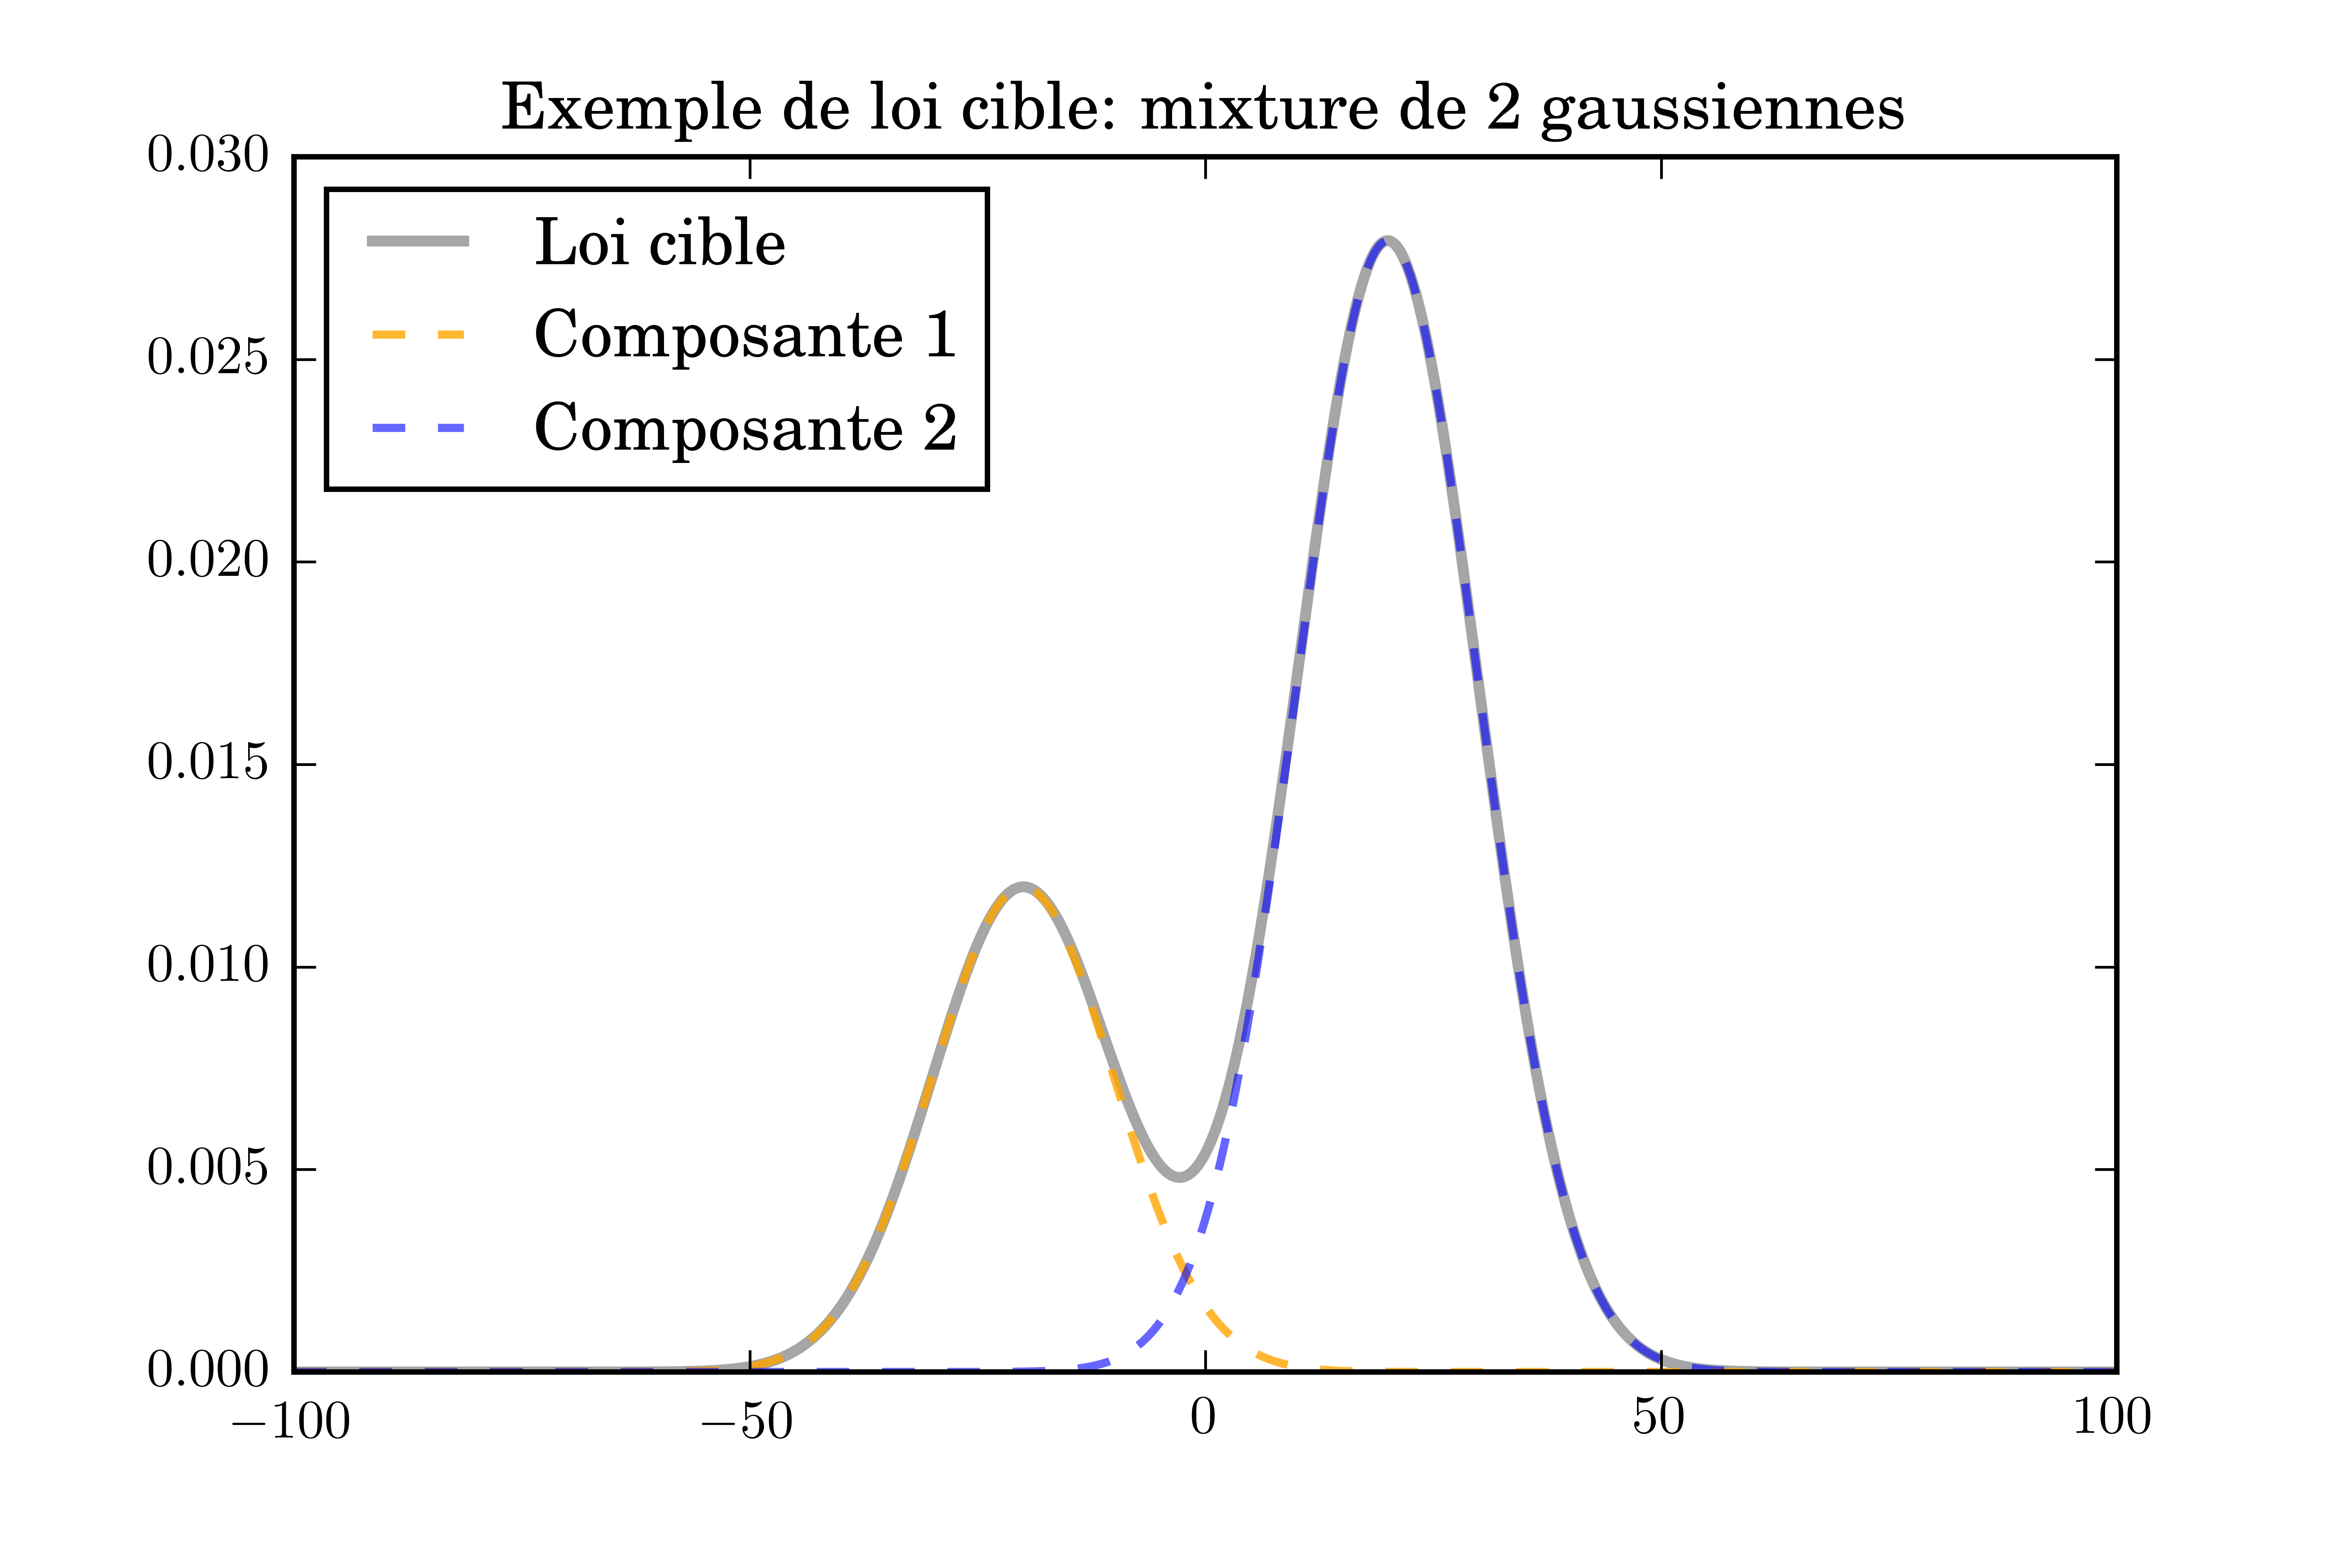
\includegraphics[scale=0.55]{courbe_pdf_mixture_1D.png}
	\caption{Exemple de loi cible: mixture de deux gaussiennes}
	\label{fig_courbe_pdf_mixture_1D}
\end{figure}


 Supposons que l'on cherche à échantillonner depuis cette distribution: nous définissons un noyau de transition de type gaussien afin d'appliquer une méthodologie de type random-walk Metropolis: 

\begin{equation}
\kernel(\VecTheta, \VecThetaCandidat ) = \mathcal{N}(\VecThetaCandidat | \VecTheta, \sigma_{K}^2)
\label{eq_noyau_gaussien}
\end{equation}

La figure \ref{fig_courbe_4_histogrammes_exemple_1} illustre ainsi l'approximation de $\pi$ grâce aux histogrammes des éléments obtenus à différentes itérations de l'algorithme. 

\begin{figure}[h!]
	\centering
	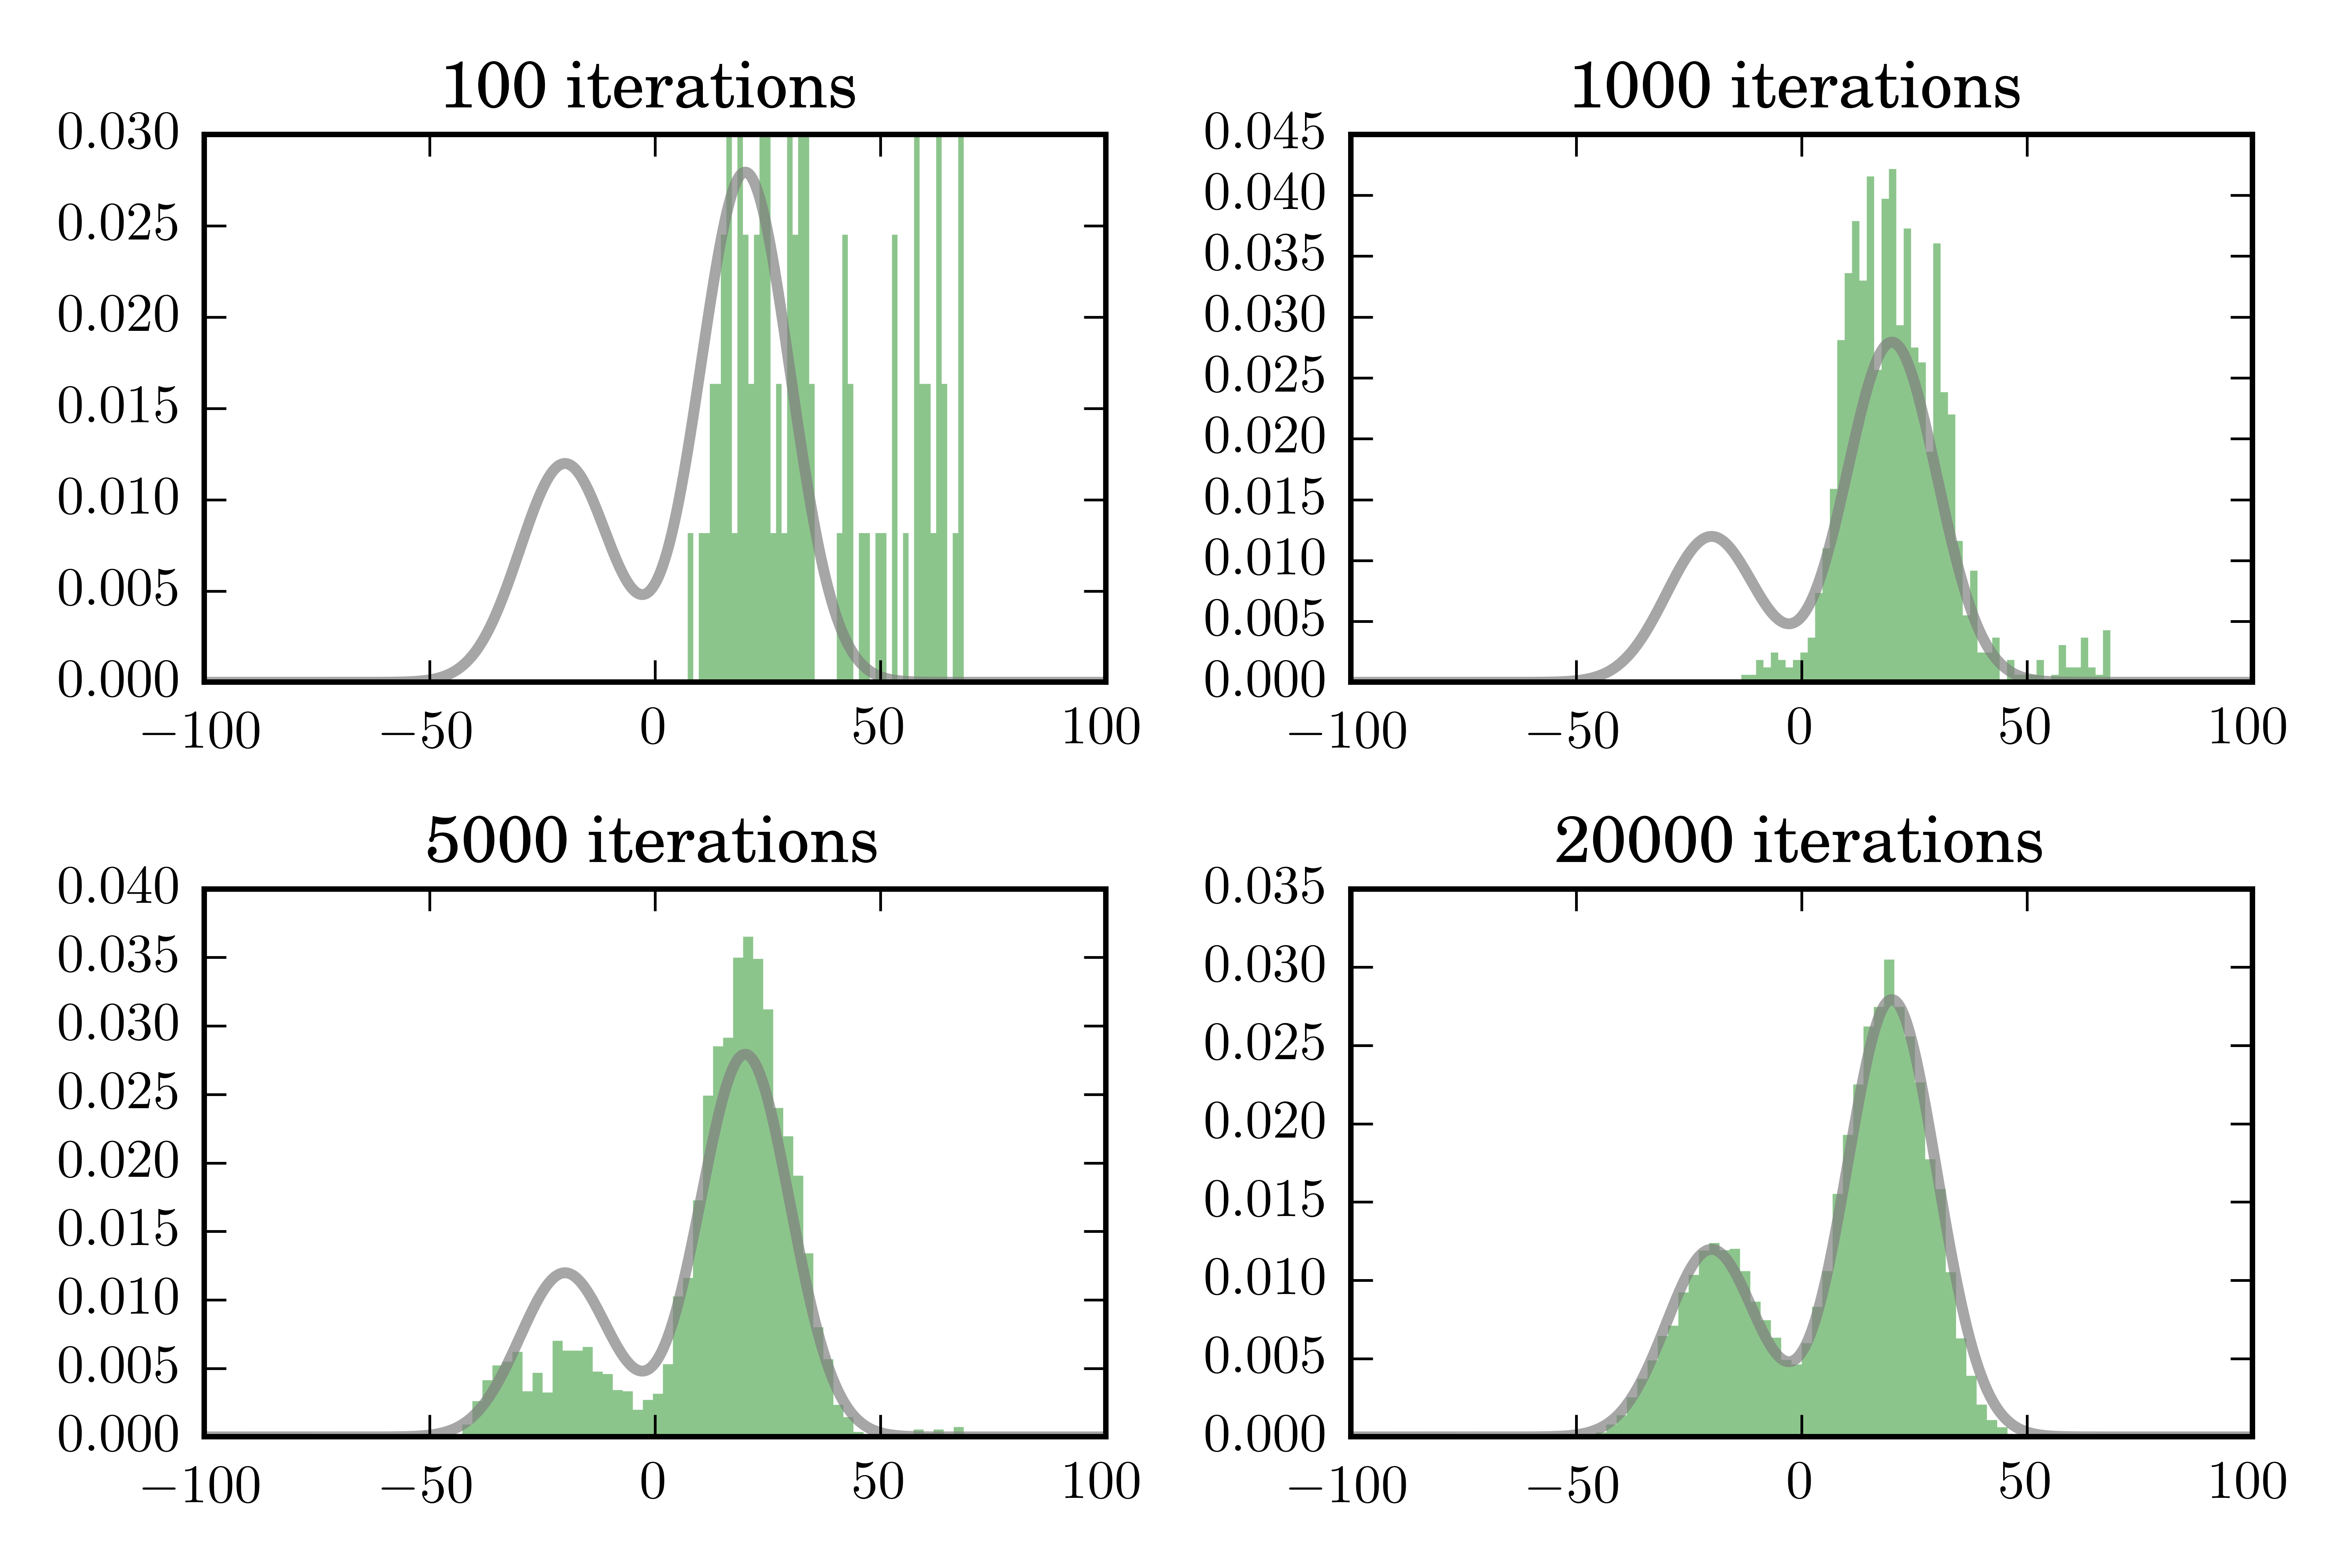
\includegraphics[scale=0.65]{courbe_4_histogrammes_exemple_1.png}
	\caption{Résultats de l'algorithme MH: histogrammes des éléments tirés (en vert) et comparaison avec la loi cible (en rouge)}
	\label{fig_courbe_4_histogrammes_exemple_1}
\end{figure}

On remarque qu'avant d'atteindre la distribution stationnaire, il existe un régime transitoire durant lequel les états de la chaîne ne permettent pas de représenter correctement la loi cible. Il est alors d'usage de ne pas tenir compte des éléments tirés durant cette période , appelée \textit{temps de chauffe} ou \textit{burn-in}. \\


\begin{figure}[h!]
	\centering
	\begin{subfigure}[t]{0.5\textwidth}
		\centering
		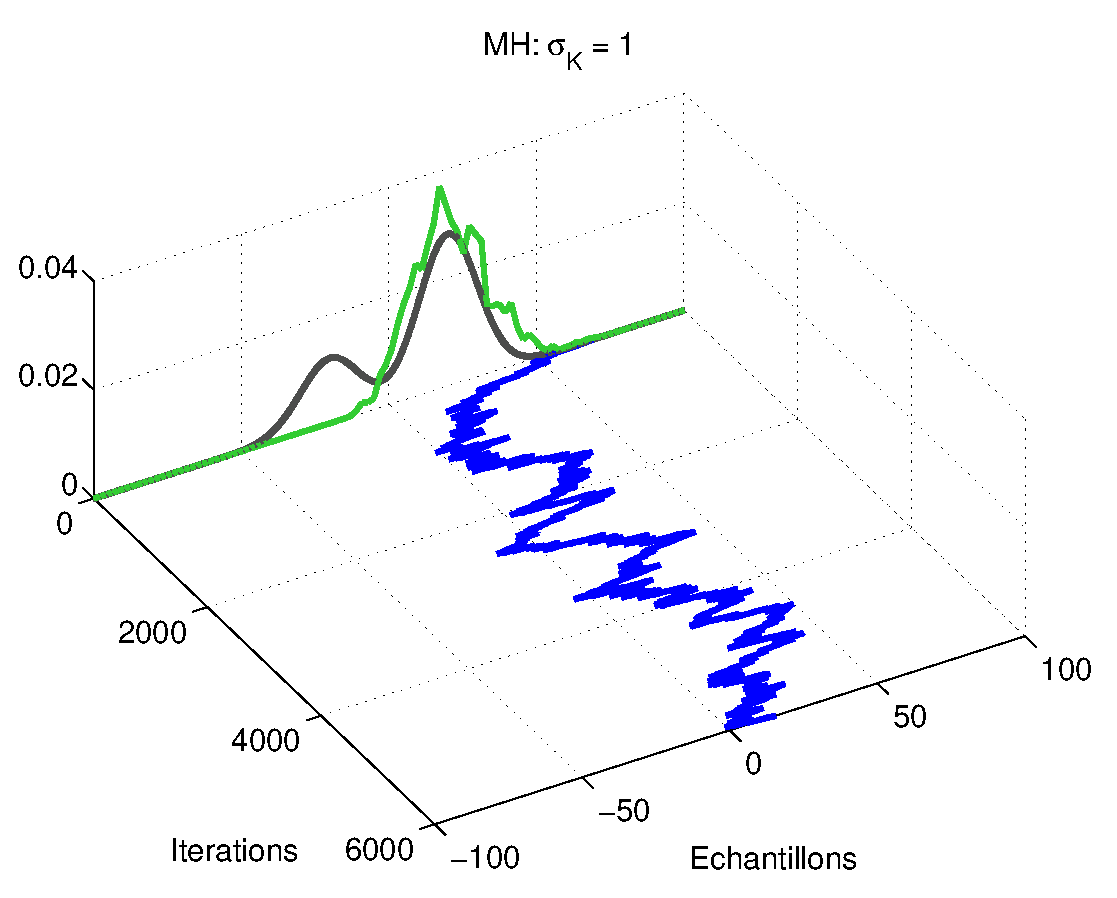
\includegraphics[width=0.9\textwidth]{courbe_MH_varKernel_1}
		\caption{}
		\label{subfig_varK_1}
	\end{subfigure}%
	~ 
	\begin{subfigure}[t]{0.5\textwidth}
		\centering
		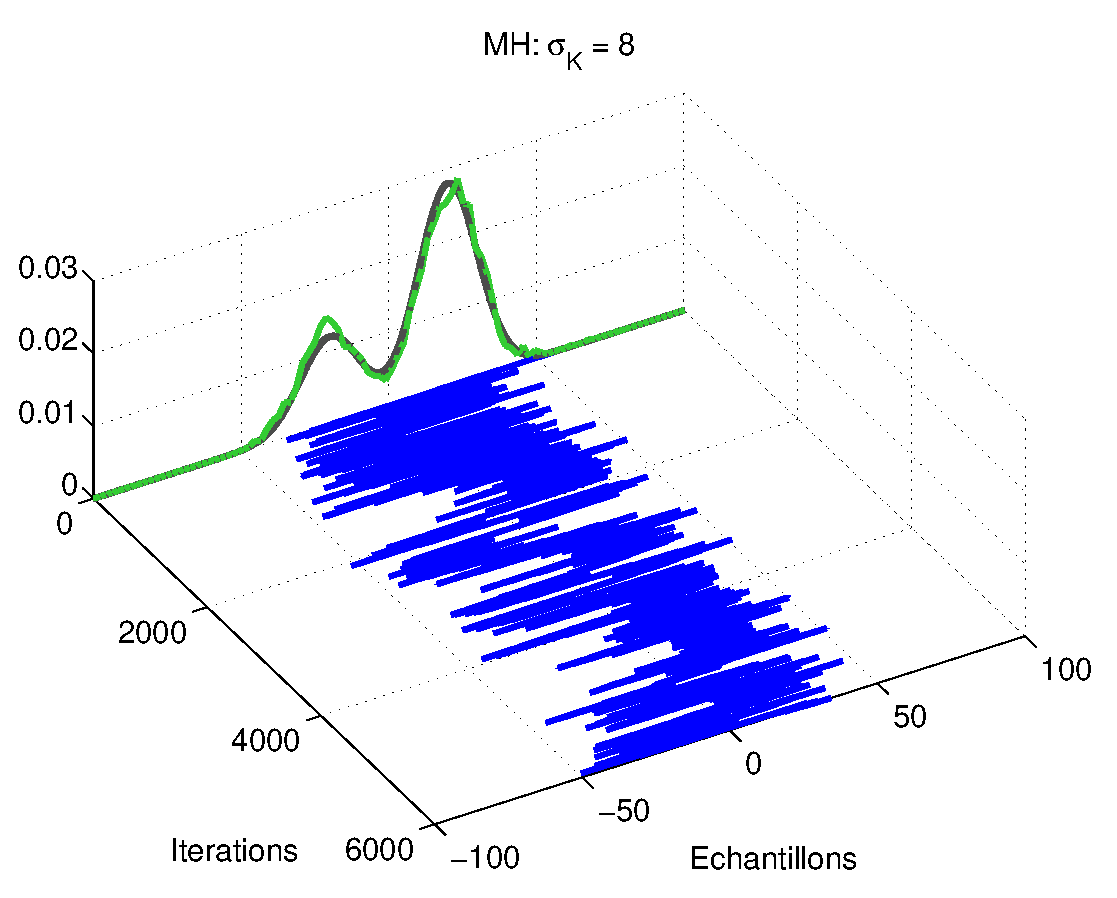
\includegraphics[width=0.9\textwidth]{courbe_MH_varKernel_8}
		\caption{}
		\label{subfig_varK_8}
	\end{subfigure}
	\begin{subfigure}{0.5\textwidth}
		\centering
		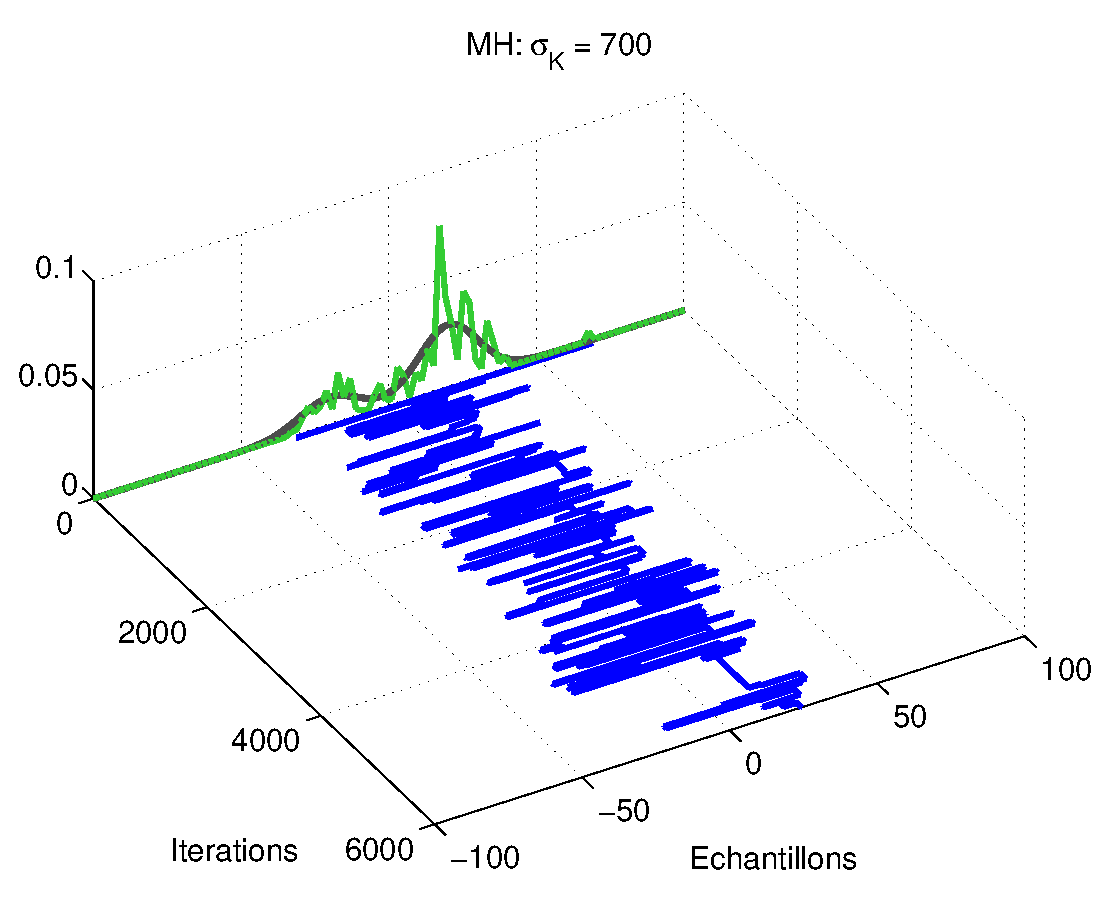
\includegraphics[width=0.9\textwidth]{courbe_MH_varKernel_700}
		\caption{}
		\label{subfig_varK_700}
	\end{subfigure}
	
	\caption{Exemples de réalisations de l'algorithme MH avec 3 valeurs différentes pour la variance du noyau de transition}
\end{figure}

La vitesse de convergence et la qualité de l'estimation sont conditionnés par deux facteurs importants: 
\begin{itemize}
	\item \textbf{l'initialisation de la chaîne}: plus l'état de départ est proche d'une valeur ayant une probabilité élevée suivant la loi cible, plus vite l'algorithme convergera. S'il est impossible de favoriser a priori une ou plusieurs valeurs de l'espace d'état, on peut simplement tirer l'état initial avec une loi uniforme sur cet espace.
	\item \textbf{le choix du noyau de transition}: dans le cas d'un random-walk Metropolis, le paramètre $\sigma_K$ reflète l'écart potentiel entre deux états consécutifs de la chaîne. Si celui-ci est trop important, les amplitudes des transitions proposées par l'algorithme deviennent trop importantes, causant un rejet fréquent des états candidats. Cela se traduit par la présence de plateaux sur la trajectoire de la chaîne, comme on le voit sur la figure \ref{subfig_varK_700}. A l'inverse, si $\sigma_K$ est choisi trop petit, l'exploration de l'espace d'état ne se fait pas de façon optimale, car la chaîne évolue beaucoup plus lentement, avec le risque de ne pas atteindre certains états représentatifs de la loi cible du fait de leur "éloignement". On retrouve ce phénomène sur la figure \ref{subfig_varK_1}, où la chaîne reste bloquée sur l'un des modes, lui empêchant d'échantillonner depuis la composante de moyenne $\mu_1 = -20$. Il faut donc choisir une valeur offrant un bon compromis, et qui permet de bien retrouver la loi cible, comme c'est le cas sur la figure \ref{subfig_varK_8}. 
\end{itemize}

\subsubsection{Echantillonneur de Gibbs}
L'échantillonneur de Gibbs a initialement été proposé dans \cite{Geman1984} puis fût repris et développé par \cite{Gelfand1990}. Il permet de passer du problème de l'échantillonnage d'un état $\VecTheta = (\theta_1, \dots, \theta_p)$ sur un espace pouvant être potentiellement de grande dimension, à une succession de sous-problèmes plus simples, en générant successivement chacun des éléments composant $\VecTheta$ à l'aide de leurs dépendances par rapport aux autres. C'est ainsi la loi conditionnelle de chaque élément de $\VecTheta$ sous la loi cible qui fait office de loi de proposition.

Le parcours des composantes de $\VecTheta$ peut se faire de façon déterministe, par exemple en les traitant dans leur ordre naturel les unes après les autres: on parle alors de \textit{balayage systématique}, ou \textit{systematic scan}, comme illustré dans l'algorithme \ref{algo_gibbs_sampler}. Une autre possibilité consiste à choisir aléatoirement cet ordre d'exploration: il s'agit du \textit{balayage aléatoire}, ou \textit{random scan}. \\

\IncMargin{1em}
\begin{algorithm}
	\SetAlgoLined
	Initialiser $\VecTheta^{(0)} = \left(\theta_1^{(0)}, \dots, \theta_p^{(0)}\right)$\;
	\For{$i = 1, \dots, N$ }{
		\For{$k = 1, \dots, p$}{
			Tirer $\theta_k^{(i)}$ depuis $p(\theta_k^{(i)} | \theta_1^{(i)}, \dots, \theta_{k-1}^{(i)}, \theta_{k+1}^{(i-1)}, \dots, \theta_p^{(i-1)})$
			}
		}
	\caption{Echantillonneur de Gibbs (balayage systématique)}
	\label{algo_gibbs_sampler}
\end{algorithm}

Pour illustrer le fonctionnement de ce type d'algorithme, nous allons chercher à échantillonner depuis une gaussienne bivariée à deux dimensions. Dans ce cas, on va donc noter $\VecTheta = (\theta_1, \theta_2)^T$, on a ainsi $\VecTheta \sim \mathcal{N}(\VecMu, \MatSigma)$ avec: 

\begin{equation}
\label{eq_caracs_gaussienne_bivariee}
\begin{split}
\VecMu &= (\mu_1, \mu_2)^T \\
\MatSigma &= \begin{pmatrix}
\sigma_{1}^2 & \corr_{\theta_1\theta_2} \sigma_1 \sigma_2 \\
 \corr_{\theta_1\theta_2} \sigma_1 \sigma_2 & \sigma_{2}^2 
\end{pmatrix}
\end{split}
\end{equation} 
où $\sigma_1^2$ et $\sigma_2^2$ sont les variances respectives de $\theta_1$ et $\theta_2$, et $\corr_{\theta_1\theta_2}$ est la corrélation entre $\theta_1$ et $\theta_2$ définie par: $$\corr_{\theta_1\theta_2} = \dfrac{\text{Cov}(\theta_1,\theta_2)}{\sigma_1\sigma_2}$$.

Le cas gaussien bivarié est relativement facile à traiter, car on sait calculer directement les expressions des lois conditionnelles, qui sont elle-mêmes gaussiennes, et qui s'écrivent sous la forme suivante\footnote{Pour un génération à un cas multivarié global et une démonstration, voir le paragraphe §4.3.4 du chapitre 4 dans \cite{Murphy2012}.}:

 \begin{equation}
 \label{eq_conditionnelles_gaussienne_bivariee}
 \begin{split}
 p(\theta_1 | \theta_2) &= \mathcal{N}\left(\theta_1 \middle\vert \mu_1 + \sigma_1 \corr_{\theta_1\theta_2} \left(\dfrac{\theta_2 - \mu_2}{\sigma_2}\right), \sigma_1^2 (1-\corr_{\theta_1\theta_2}^2)\right) \\
 p(\theta_2 | \theta_1) &= \mathcal{N}\left(\theta_2 \middle\vert \mu_2 + \sigma_2 \corr_{\theta_1\theta_2} \left(\dfrac{\theta_1 - \mu_1}{\sigma_1}\right), \sigma_2^2 (1-\corr_{\theta_1\theta_2}^2)\right)
 \end{split}
 \end{equation}
 
\begin{figure}[h!]
	\centering
	\begin{subfigure}[t]{0.5\textwidth}
		\centering
		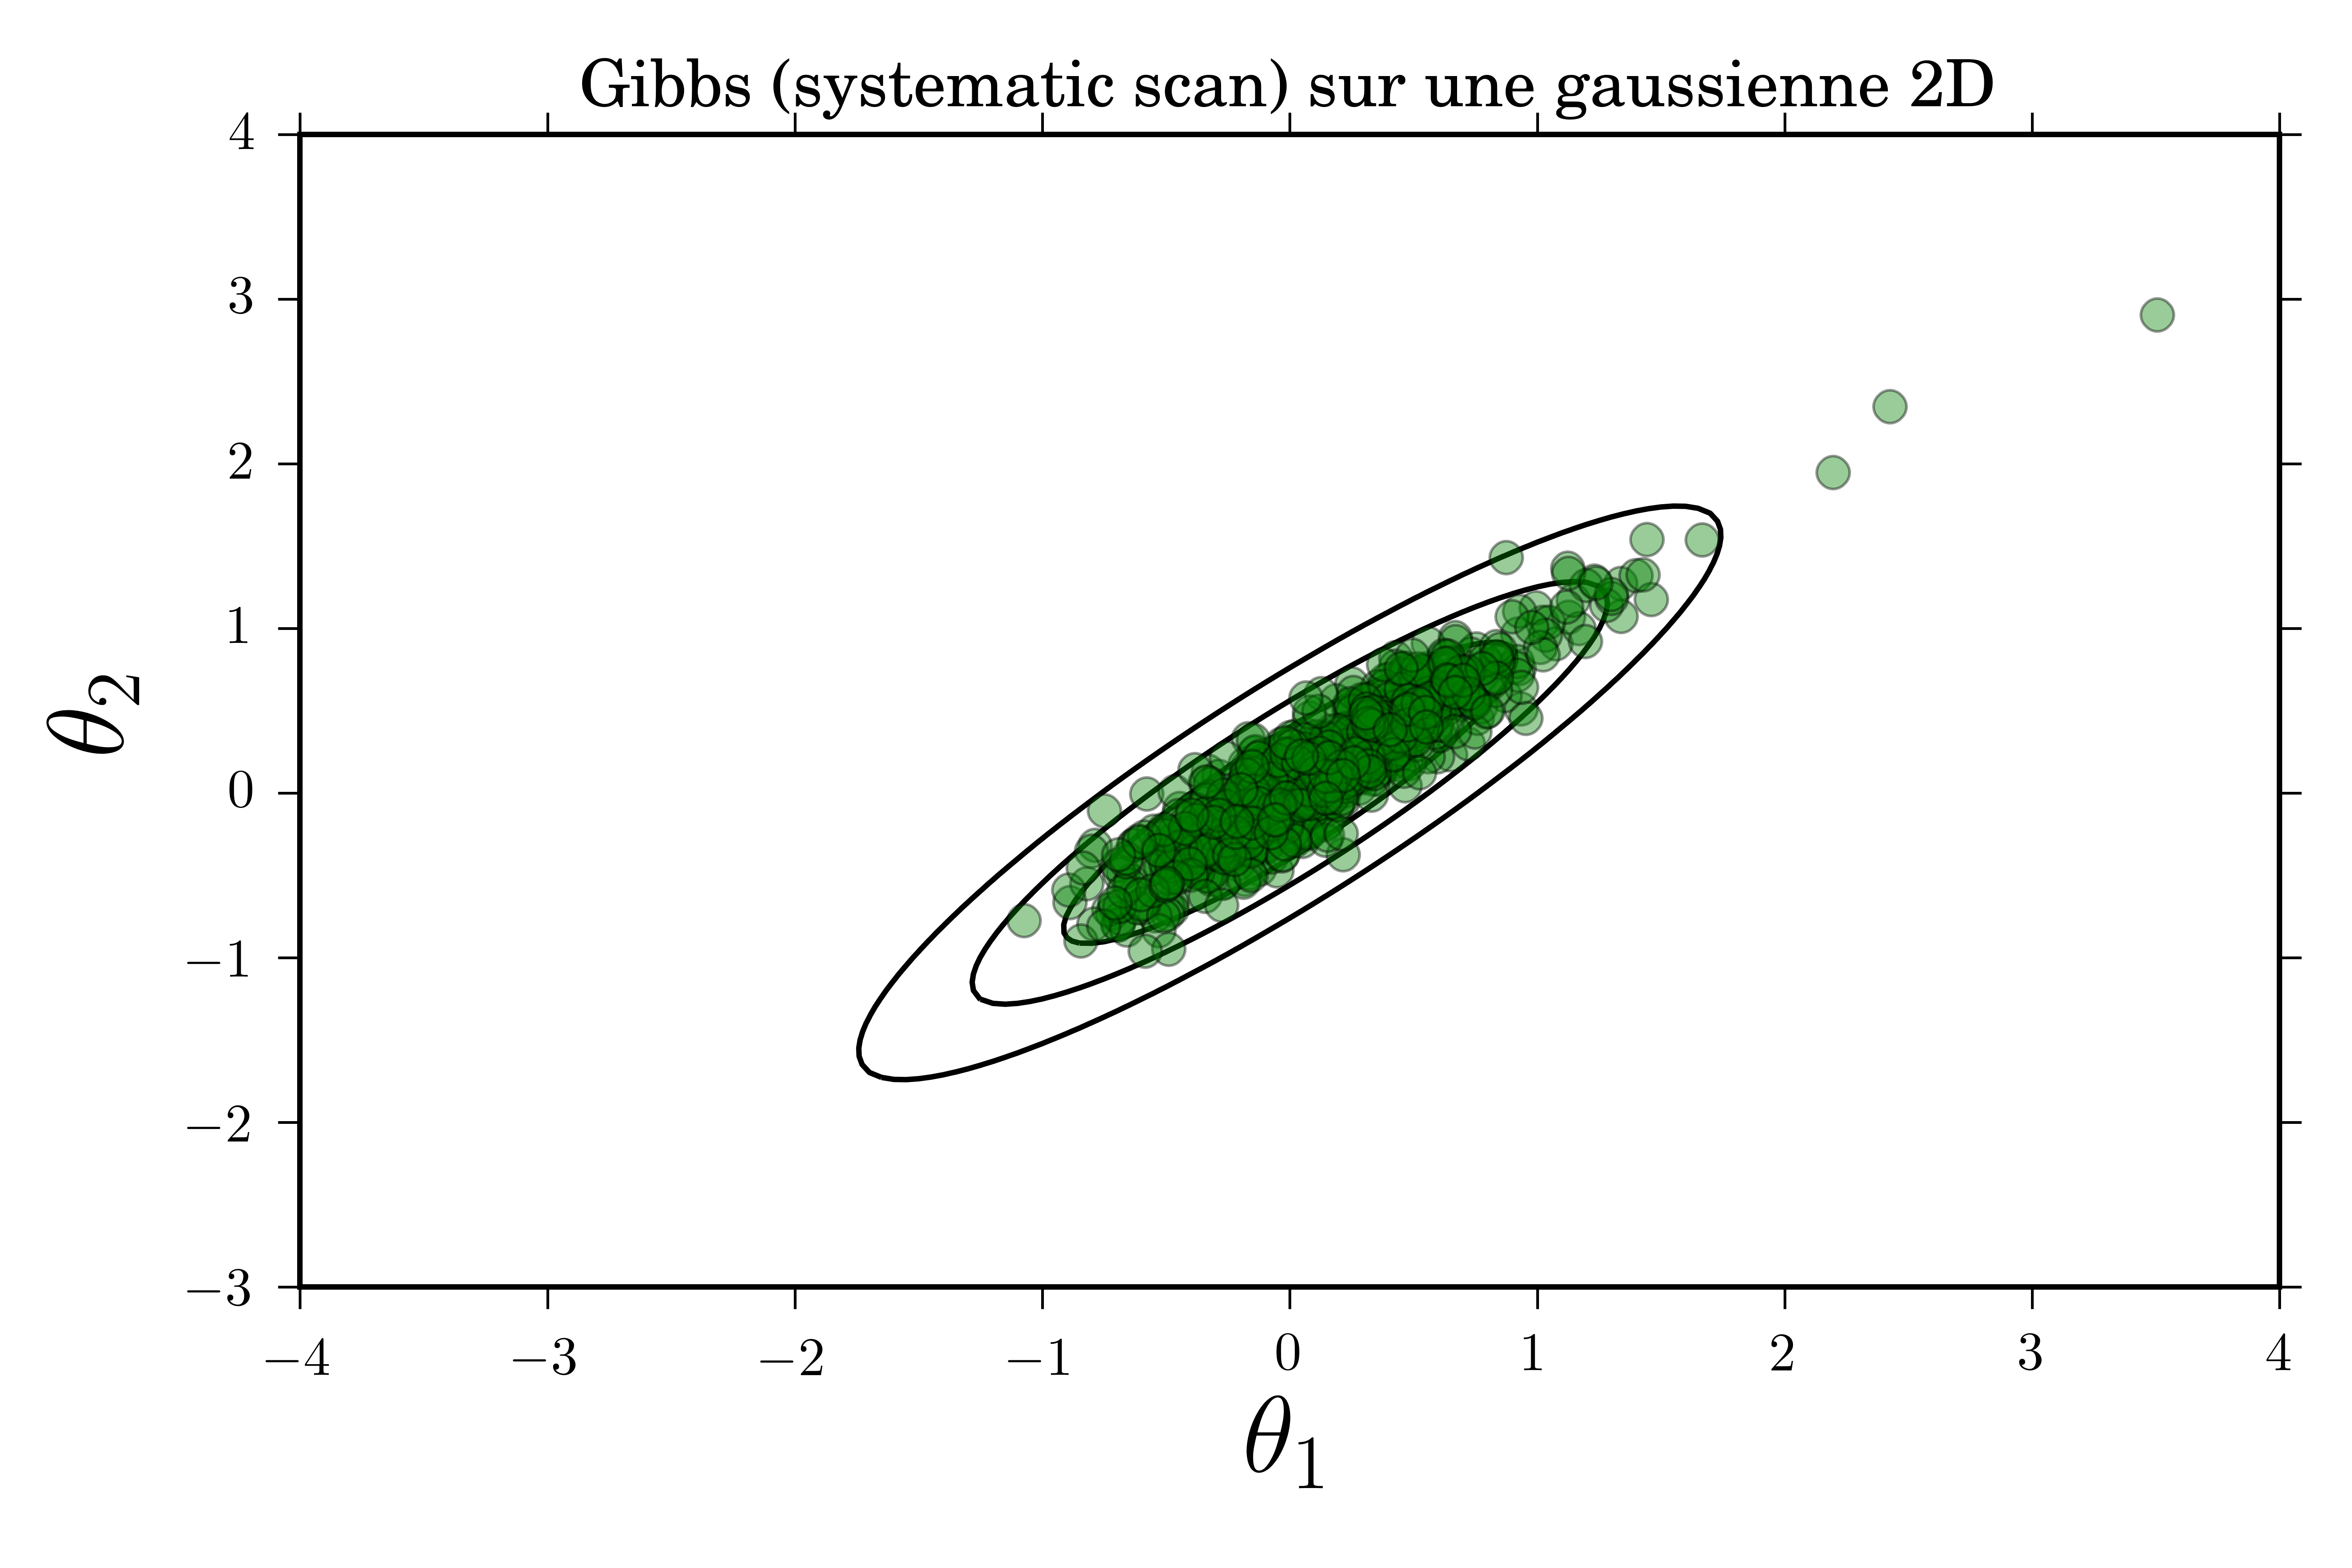
\includegraphics[width=0.9\textwidth]{courbe_gibbs_gaussienne_2D.png}
		\caption{}
		\label{subfig_gibbs_all}
	\end{subfigure}%
	~ 
	\begin{subfigure}[t]{0.5\textwidth}
		\centering
		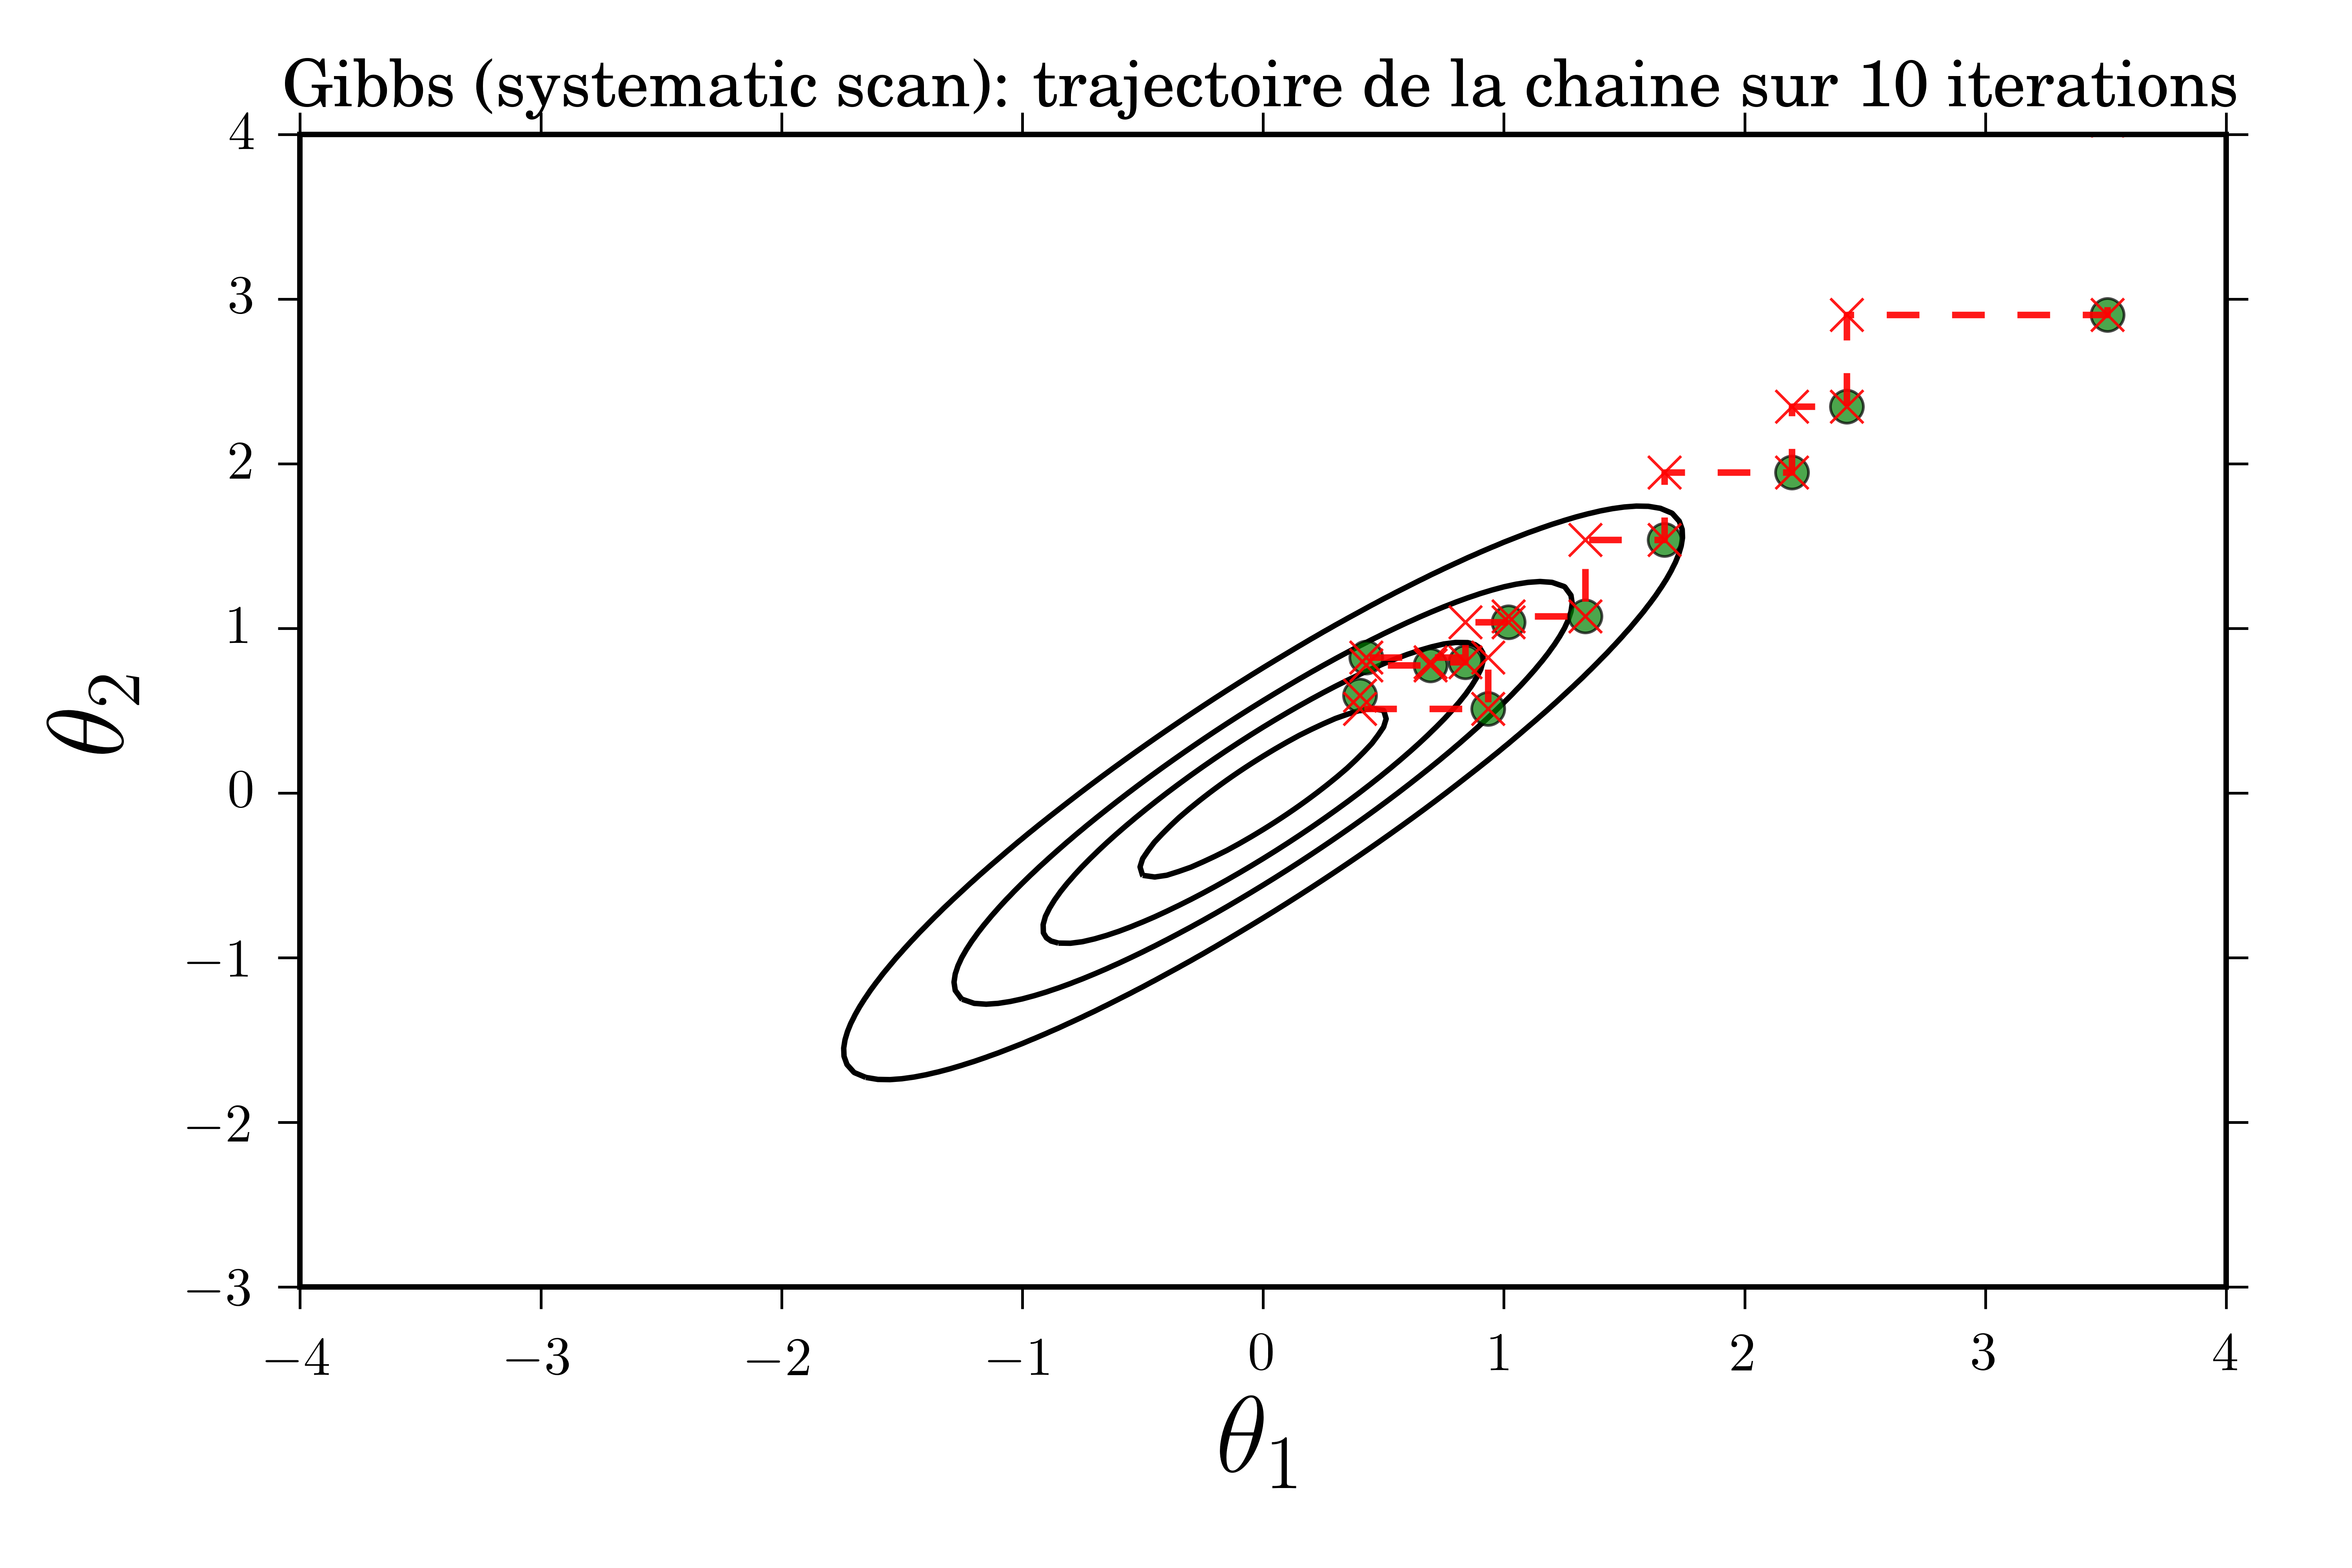
\includegraphics[width=0.9\textwidth]{courbe_gibbs_trajectoire_10_iterations.png}
		\caption{}
		\label{subfig_gibbs_10}
	\end{subfigure}
	\caption{Illustration de l'échantillonneur de Gibbs pour une loi cible de type gaussienne bivariée (en noir) avec le résultat sur 800 itérations (a) et sur 10 itérations avec trajectoire (b)}
\end{figure}

La figure \ref{subfig_gibbs_10} reflète bien le comportement de l'algorithme: la trajectoire de la chaîne (en pointillés gris) met en évidence le fait que les composantes de $\VecTheta$ sont évaluées une par une. 

Cette famille d'algorithmes, contrairement à l'approche MH, n'effectue pas de sélection des états échantillonnés, et exploite ainsi toute l'information générée lors de la simulation. Cependant, elle nécessite de pouvoir échantillonner depuis les lois conditionnelles, ce qui n'est pas souvent facile. Aussi, dans ces cas-là, une variante consiste à avoir recours à une itération de type MH avec une loi de proposition choisie par l'utilisateur: cette méthode porte le nom de \textit{Metropolis-Within-Gibbs} (MWG).\\

 
 \subsection{Echantillonnage d'importance classique (IS)}
 
 Avec les approches MCMC, on a vu qu'il existait plusieurs façons de traiter les éléments générés par la loi de proposition: on peut les soumettre à une procédure d'acceptation-rejet, ou alors tous les garder. Une autre vision du problème est proposée par les méthodes dites d'échantillonnage d'importance, ou \textit{importance sampling} (IS), où l'utilisation de poids permettent de quantifier la pertinence de chaque élément. Dans la suite de ce paragraphe, nous emploierons le terme de \textit{particules} afin de désigner les éléments d'un échantillon.\\
 
 L'idée de départ des méthodes IS est de chercher à approximer des intégrales de la forme : 
 
 \begin{equation}
  I = \mathbb{E}_\pi[f(\VecTheta)] = \int f(\VecTheta)\pi(\theta)d\VecTheta
  \label{eq_IS_integrale_1}
 \end{equation}
 
 Pour cela, on définit une loi de proposition $\propFonc$ permettant de réécrire l'équation \eqref{eq_IS_integrale_1} sous la forme:
 
 \begin{equation}
\mathbb{E}_\pi[f(\VecTheta)] = \int  f(\VecTheta) \dfrac{\pi(\theta)}{\propFonc(\VecTheta)}\propFonc(\VecTheta)d\VecTheta = \int  f(\VecTheta) w(\VecTheta) \propFonc(\VecTheta)d\VecTheta 
\label{eq_IS_integrale_2}
 \end{equation}
 où $w(\VecTheta) = \dfrac{\pi(\VecTheta)}{\propFonc(\VecTheta)}$ définit le vecteur des \textit{poids d'importance}.  La forme de l'intégrale obtenue permet alors de dire que:
 
\begin{equation}
\mathbb{E}_\pi[f(\VecTheta)] = \mathbb{E}_\propFonc[f(\VecTheta)w(\VecTheta)] 
\label{eq_IS_integrale_2_1}
\end{equation}

D'après la loi forte des grands nombres, $\sum\limits_{i=1}^N f(\VecTheta^{(i)}) w^{(i)}$ converge presque sûrement vers  $\mathbb{E}_\varphi[f(\VecTheta)w(\VecTheta)]$ pour $N \rightarrow + \infty$. En associant cela avec l'équation \eqref{eq_IS_integrale_2_1}, on obtient ainsi:
 
 \begin{equation}
 \mathbb{E}_\pi[f(\VecTheta)] \simeq I_N = \dfrac{1}{N}\sum\limits_{i=1}^N f(\VecTheta^{(i)})  w^{(i)}
 \label{eq_IS_integrale_3}
 \end{equation}
 
 Dans notre contexte, l'équation \eqref{eq_bayes_proportionnalite} nous rappelle que la loi cible n'est connue qu'à une constante près: pour en tenir compte, il est nécessaire de normaliser les poids d'importance. En écrivant : 
 
 \begin{equation}
 \forall i \in \{1, \dots, N\}, ~ \poidsNorm^{(i)} = \dfrac{w^{(i)}}{\sum\limits_{i=1}^N w^{(i)}}
 \label{eq_IS_poids_normalises}
 \end{equation}
 on garantit bien que toutes les valeurs de $\VecPoidsNorm$ sont comprises entre 0 et 1. \\
 
 En reprenant l'équation \eqref{eq_IS_integrale_3}, on peut alors obtenir une approximation de la loi cible, qui s'écrit:
 
 \begin{equation}
 \pi(\VecTheta) \simeq \sum\limits_{i=1}^N \poidsNorm(\VecTheta^{(i)})\delta_{\VecTheta^{(i)}}(\VecTheta)
 \label{eq_IS_approximation_loi_cible}
 \end{equation}

L'équation \eqref{eq_IS_approximation_loi_cible} permet ainsi d'obtenir des particules pondérées de la loi cible. Pour cela, il faut choisir une loi de proposition $\propFonc$ qui soit suffisamment proche de la loi cible, dont le support englobe celui de cette dernière, et à partir de laquelle on puisse échantillonner facilement. \\

\begin{figure}[h!]
	\centering
	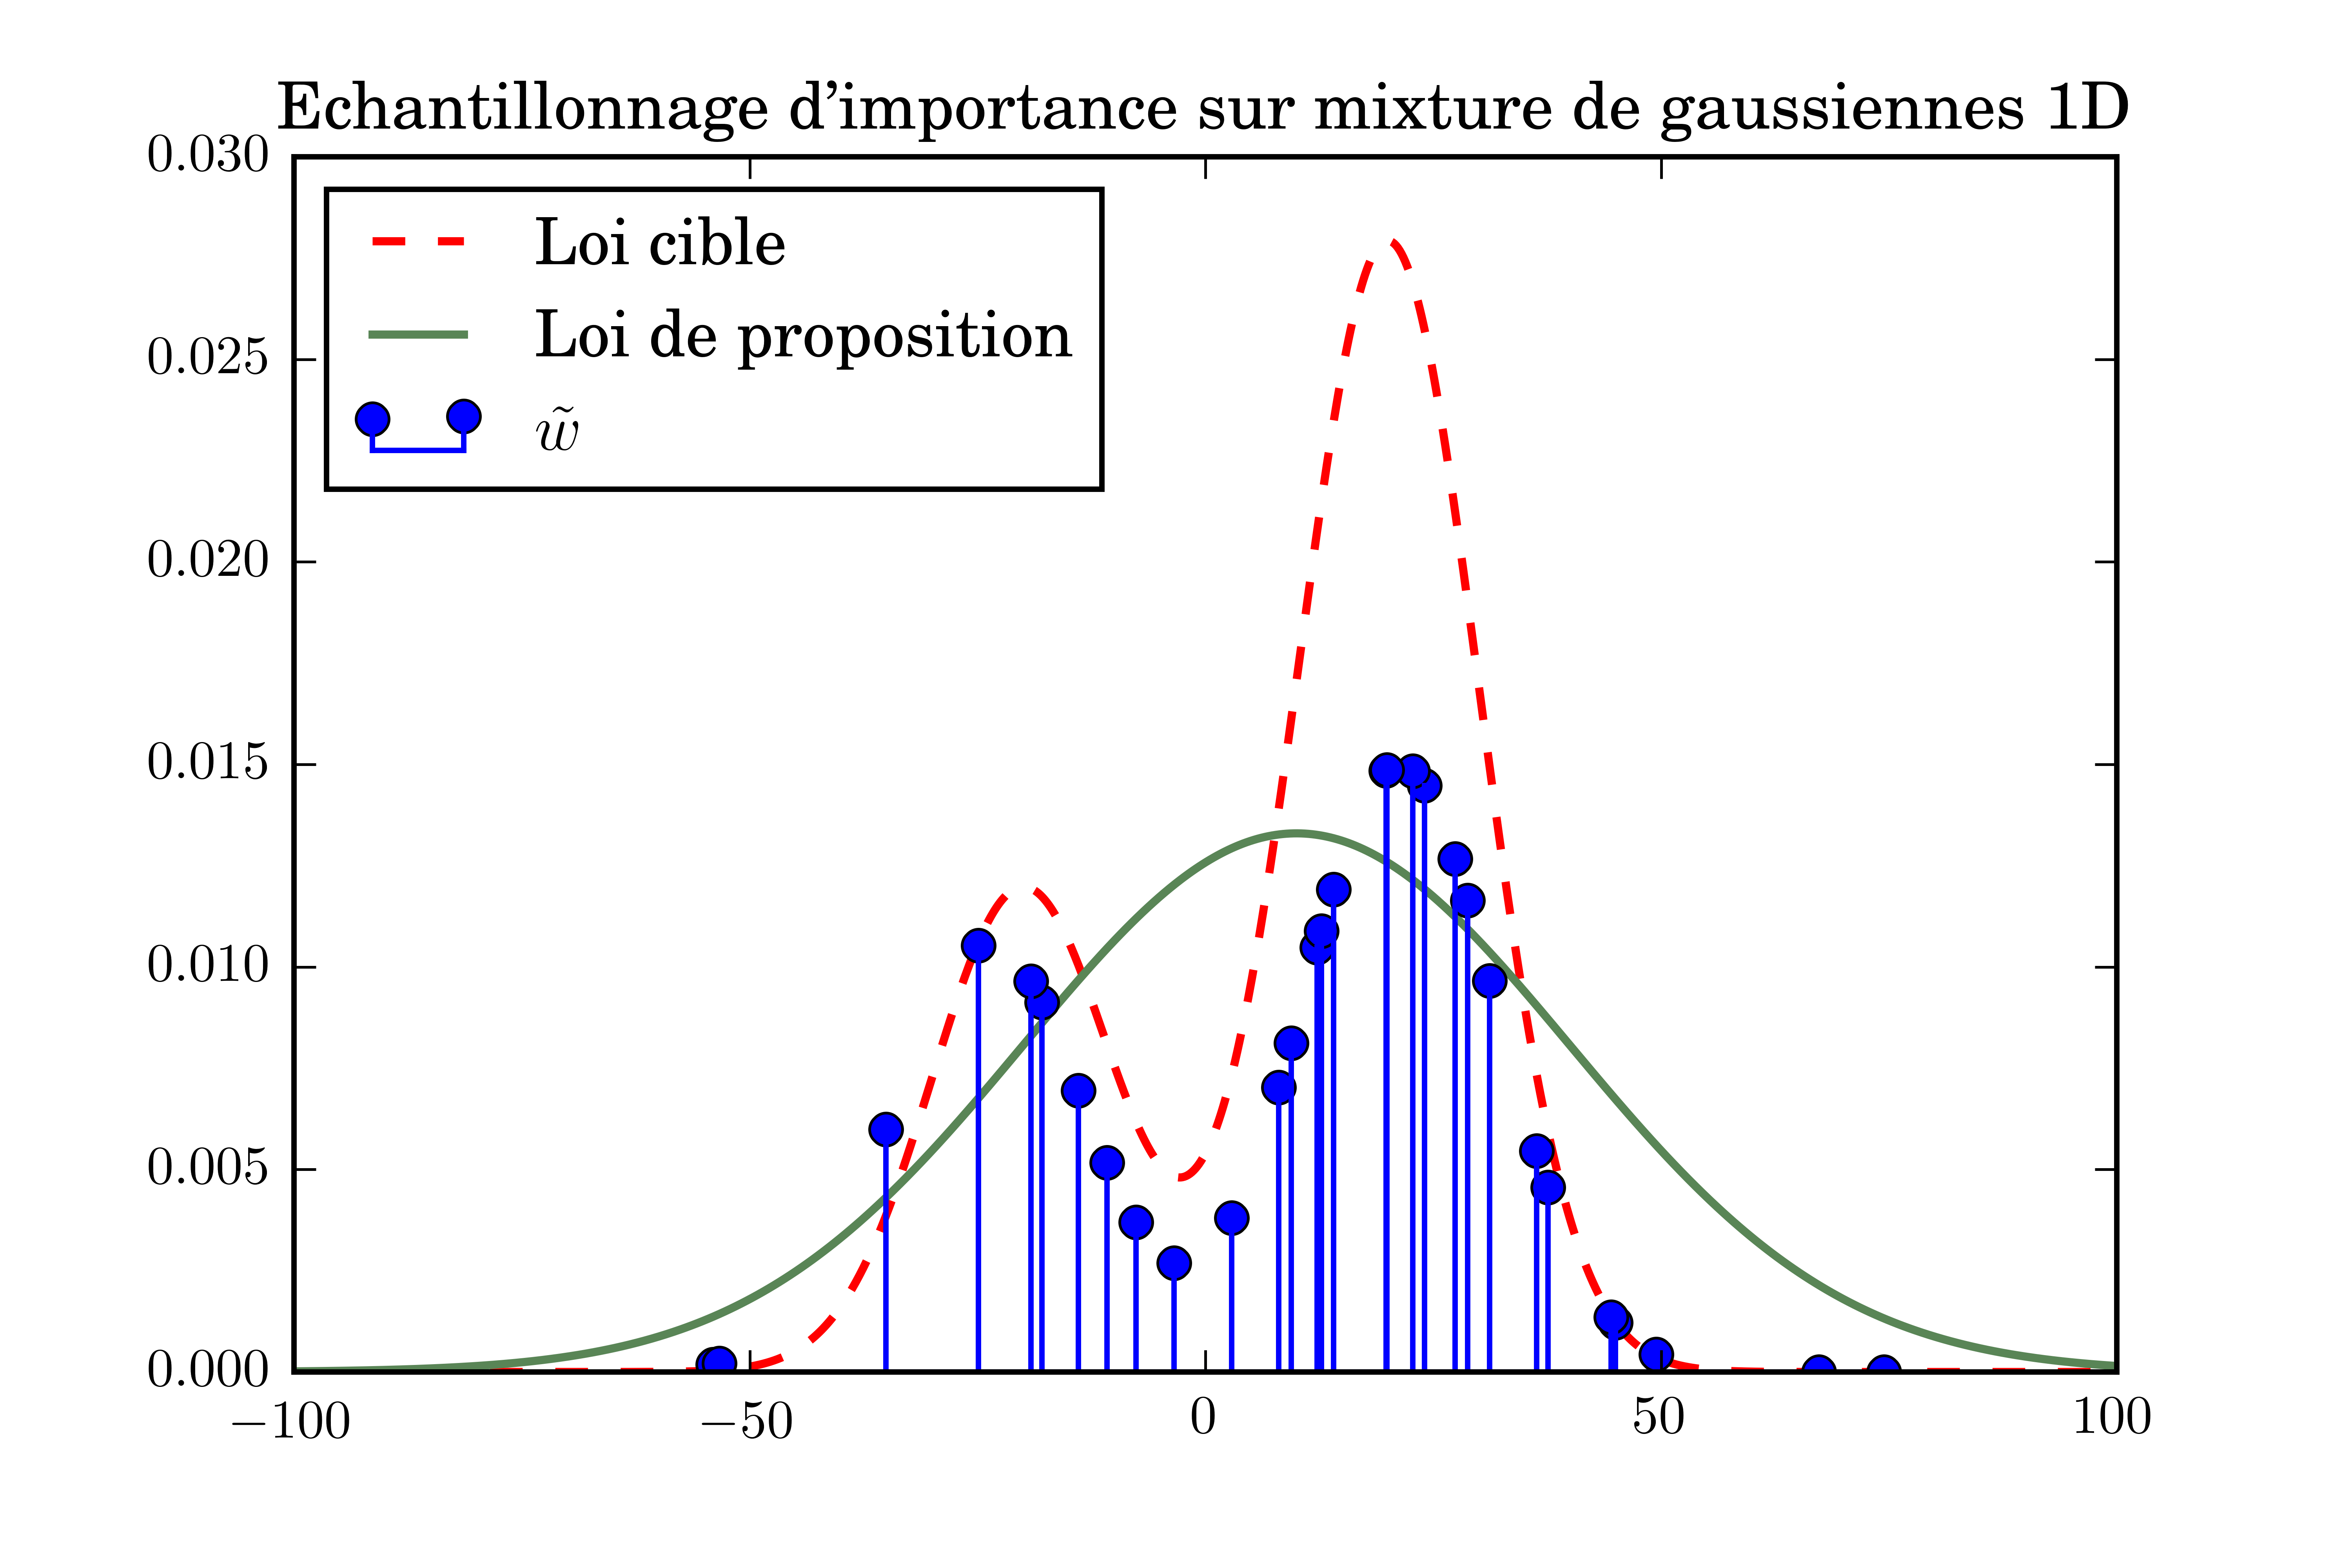
\includegraphics[scale=0.8]{courbe_IS_gmm_1D.png}
	\caption{Calcul des poids d'importance normalisés  (en bleu) sur les 30 premiers éléments d'un vecteur de 1000 particules , avec la loi cible de la figure \ref{fig_courbe_pdf_mixture_1D} (pointillés rouges) et une loi de proposition $\mathcal{N}(\mu = 10, \sigma = 30)$ (en vert).  }
	\label{fig_IS_gmm_1D}
\end{figure}

En reprenant l'exemple de la mixture de deux gaussiennes utilisé précédemment (voir équation  \eqref{eq_mixture_2_gaussiennes_1D"}), on observe sur la figure \ref{fig_IS_gmm_1D} que si la loi de proposition est bien choisie, alors on obtient une bonne approximation de la loi cible. Le choix de cette loi est en fait un point crucial des méthodes IS, et présente certaines difficultés s'il est impossible d'associer "intuitivement" une distribution $\varphi$ à une loi cible $\pi$, par exemple lorsqu'on se place dans des grandes dimensions, ou plus généralement lorsque $\pi$ est trop complexe pour être rattachée à une famille de lois connue. 

Une loi de proposition mal choisie peut engendrer un ralentissement de la convergence de l'algorithme, voire une impossibilité à approximer correctement la loi cible. Par exemple, sur la figure \ref{courbe_IS_bad_proposal}, la nouvelle loi de proposition ne permet pas d'échantillonner correctement depuis le premier mode à -20.

\begin{figure}[h!]
	\centering
	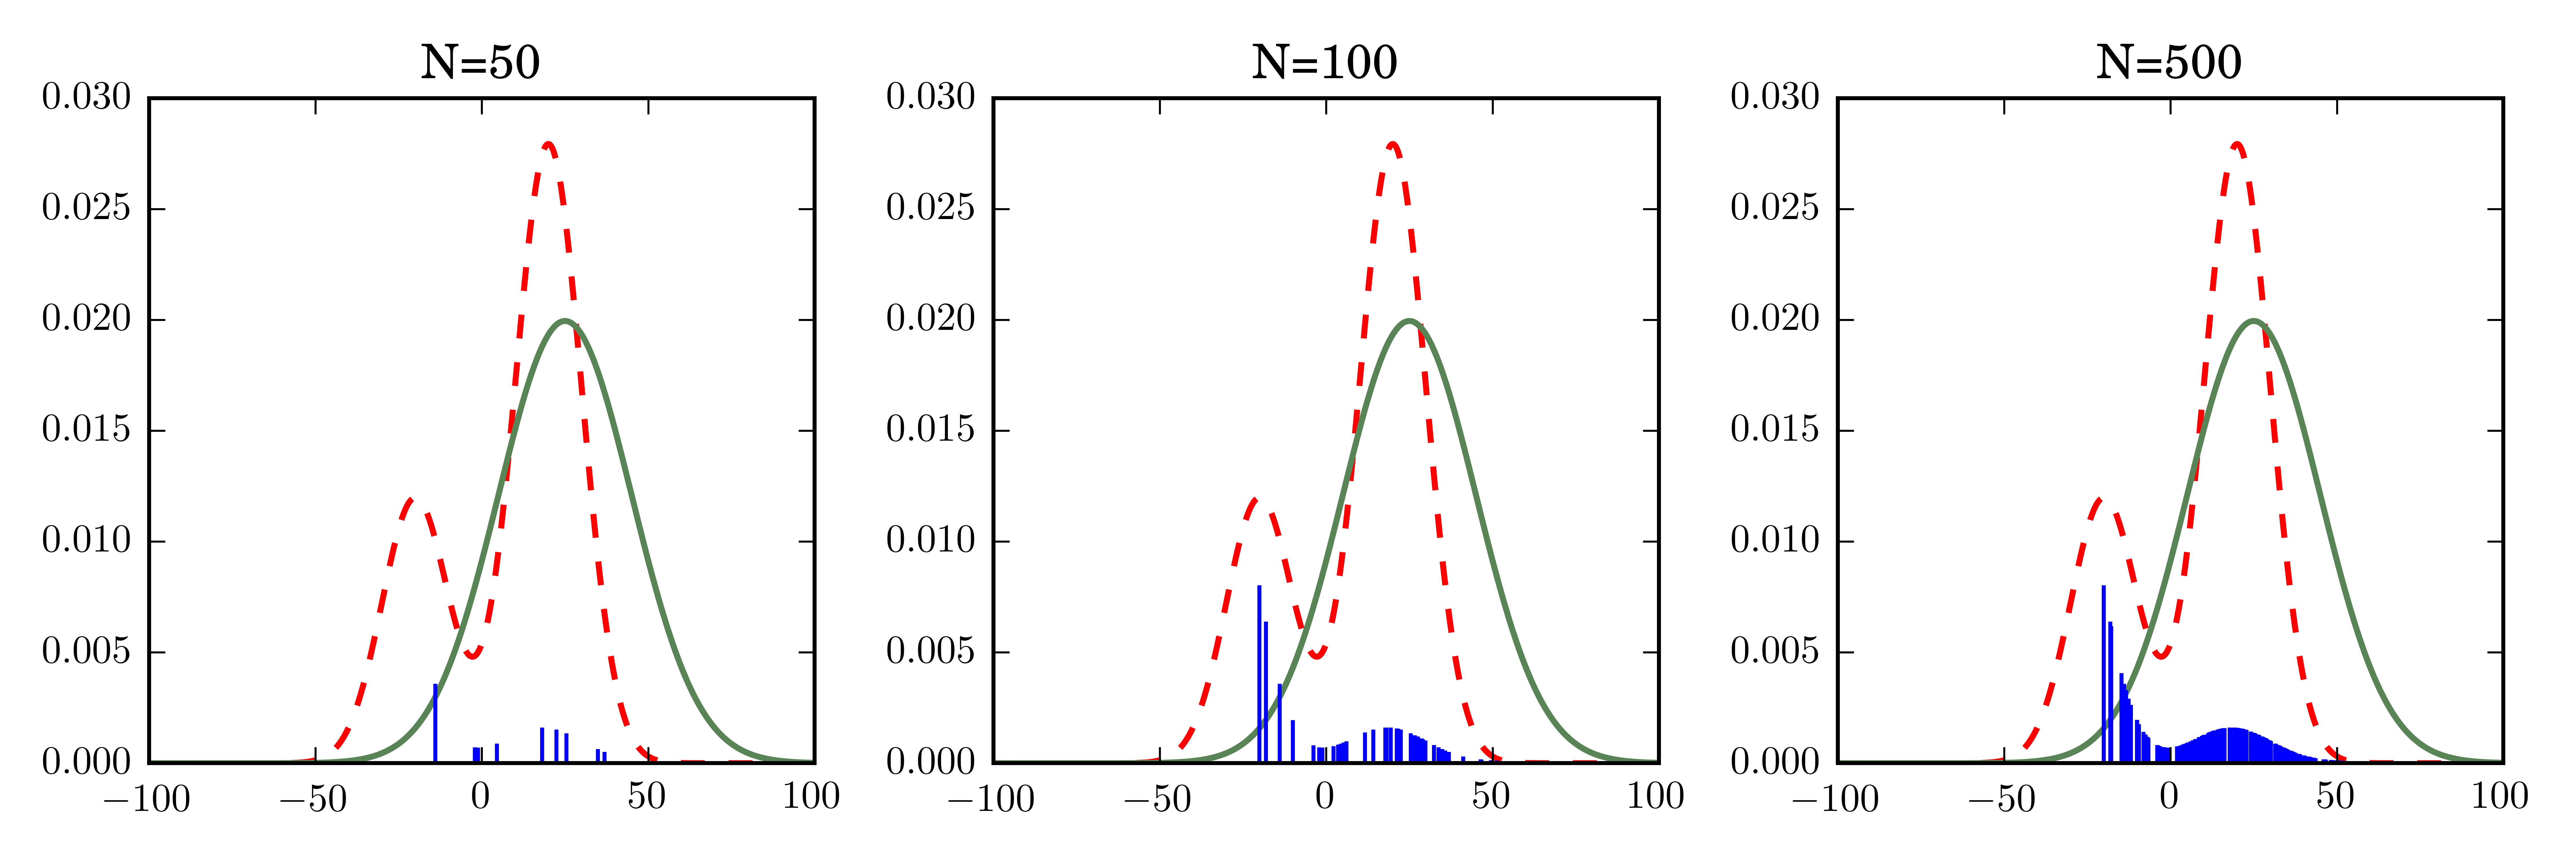
\includegraphics[width=0.99\textwidth]{courbe_IS_bad_proposal.png}
	\caption{IS pour une loi de proposition $\mathcal{N}(\mu=25, \sigma=20)$ à différentes étapes de l'échantillonnage.}
	\label{courbe_IS_bad_proposal}
\end{figure}

On observe également que les valeurs des poids des particules tirés autour du mode à -20 sont trop élevées par rapport à ce qui est attendu. On remarque aussi qu'un petit nombre de particules agrège les valeurs les plus importantes des poids, alors que la majorité restante détient des poids de faible valeur. Ce déséquilibre de répartition est plus généralement connu sous le nom de \textit{dégénérescence des poids}. La métrique permettant de quantifier ce phénomène, et de facto évaluer les performances de la loi de proposition, est appelée \textit{Effective Sample Size} ($\ESS$), et se calcule selon la formule suivante:

\begin{equation}
\mathbb{ESS} = \dfrac{\left(\sum\limits_{i=1}^N w^{(i)}\right)^2}{\sum\limits_{i=1}^N \left(w^{(i)}\right)^2}
\label{eq_def_ESS}
\end{equation}

Dans le cas le plus extrême où une unique particule à un poids égal à 1 et toutes les autres ont un poids nul, on a $\ESS = 1$. Plus sa valeur croît, plus la loi de proposition est proche de la loi cible, le cas parfait étant $\ESS = N$ où $\propFonc$ et $\pi$ sont identiques.\\

Une façon de contourner le problème de la dégénérescence consiste à ré-échantillonner sur les points où les poids d'importance sont élevés: cette méthode fût développée par \cite{Rubin1988} sous le nom d'algorithme \textit{Sampling Importance Resampling} (SIR). Une autre alternative revient à moduler la loi de proposition en fonction des valeurs de poids obtenues, ce qui est possible grâce aux méthodes d'\textit{échantillonnage d'importance adaptatives} sur lesquelles nous allons à présent nous pencher.\\

\subsection{Méthodes d'échantillonnage d'importance adaptatif}

Le facteur-clé de la performance d'un algorithme de type IS réside dans l'utilisation d'une bonne loi de proposition: il paraît donc naturel d'envisager des méthodes permettant l'ajustement de cette loi pour qu'elle permette une bonne approximation de la loi cible. \\

Les travaux présentés dans \cite{Cappe2004} illustrent une première approche, qui peut être vue comme une version itérative de l'IS visant à adapter la loi de proposition afin de la rapprocher au mieux de la loi cible. Plus précisément, à chaque itération $k$: 
\begin{enumerate}
	\item on tire un échantillon $\VecTheta_k = (\theta_{1,k}, \dots, \theta_{N_p,k})$ de particules obtenues par une perturbation stochastique qui revient à appliquer un noyau de transition de type "marche aléatoire" sur chacun des $\theta_{1,k-1}, \dots, \theta_{N_p,k-1}$, à la façon d'une chaîne de Markov,
	\item on calcule le vecteur des poids d'importance normalisés $\VecPoidsNorm_t$ de ces particules,
	\item on génère un nouvel échantillon $(\tilde{\theta}_{1,k}, \dots, \tilde{\theta}_{N_p,k})$ obtenu par \textit{resampling} de $ (\theta_{1,k}, \dots, \theta_{N_p,k})$ en utilisant les poids $\VecPoidsNorm_k$.

\end{enumerate}

Le point 3. donne le résultat de l'algorithme à l'itération $k$, à savoir un vecteur de particules ajustées pour être proche de la loi cible. A partir de là, on peut ré-itérer en appliquant de nouveau une perturbation sur ce vecteur, et ainsi de suite. 

A la différence des algorithmes MCMC, on ne génère pas qu'un seul élément par itération comme c'est le cas pour chaque nouvel état de la chaîne de Markov, mais plutôt une nouvelle population issue d'une loi de proposition différente de l'itération précédente, d'où le nom de \textit{Population Monte Carlo} (PMC) attribué à cette famille de méthodes.\\

\cite{Douc2007} formalise le concept d'adaptation de la loi de proposition en la définissant comme étant un mélange de $D$ noyaux fixes $\propFonc_1, \dots, \propFonc_D$ défini par : 

\begin{equation}
\propFonc_\alpha(\VecTheta, \VecThetaCandidat) = \sum\limits_{d=1}^D\alpha_d \propFonc_d(\VecTheta, \VecThetaCandidat)
\label{eq_PMC_D_Kernel}
\end{equation}
où les $\alpha_d$ définissent les \textit{facteurs d'influence} des composantes respectives $\propFonc_d$, et sont tels que $$\sum\limits_{d=1}^D \alpha_d = 1$$. La démarche proposée, portant le nom de \textit{D-kernel PMC}, consiste à ajuster les valeurs des $\alpha_d$ à chaque itération d'un algorithme PMC, sur la base d'un critère de performance visant à minimiser l'écart statistique entre la distribution de proposition et la loi cible. Un tel écart peut être quantifié par la \textit{divergence de Kullback-Leibler} (KL)  $D(\pi || \propFonc_\alpha )$, définie par : 


\begin{equation}
D(\pi || q_\alpha ) = \int \log\left(\dfrac{\pi(\VecTheta)}{q_\alpha(\VecTheta)}\right)\pi(\VecTheta)d\VecTheta
\label{eq_definition_KL}
\end{equation}

\cite{Cappe2008} propose une extension de ces travaux en introduisant une méthode appelée \textit{M-PMC} reposant sur le même type de critère de performance, mais visant cette fois à étendre la phase d'adaptation à tous les paramètres de la mixture $q_\alpha$, sans se limiter aux seuls $\alpha_d$. La loi de proposition peut alors s'écrire sous la forme suivante:

\begin{equation}
\propFonc_{(\alpha,\nu)}(\VecTheta) = \sum\limits_{d=1}^D\alpha_d \propFonc_d(\VecTheta |\nu_d)
\label{eq_M_PMC_kernel}
\end{equation}
où $\nu_d$ représente les paramètres de la $d$-ième composante de la loi de proposition.

La procédure d'adaptation qui en découle s'inspire de l'algorithme dit d'\textit{Expectation-Maximization} (EM) pour construire les équations de mise à jour des $\nu_d$ : en effet, le fait de minimiser l'équation \eqref{eq_definition_KL} équivaut ici  à maximiser la grandeur : 

\begin{equation}
\int \log\left(\sum\limits_{d=1}^D \alpha_d \propFonc_d(\VecTheta| \nu_d)\right)\pi(\VecTheta)d\VecTheta
\label{eq_KL_pour_EM}
\end{equation} 

On se ramène ainsi à un problème similaire à celui du calcul d'un estimateur du maximum de vraisemblance pour un modèle de mixture, d'où l'emploi d'une méthode de type EM. 

Ce type de méthode est particulièrement approprié si on choisit la loi de proposition comme étant une mixture de gaussiennes multivariées, i.e. dont la densité en dimension $p$ prend la forme suivante : 

\begin{equation}
\forall d = 1, \dots, D, ~ q_d(\VecTheta|\nu_d) = \dfrac{1}{\left((2\pi)^p\det \Sigma_d\right)^{1/2}}\exp\left(-\dfrac{1}{2}(\VecTheta - \mu_d)^T \Sigma_d^{-1}(\VecTheta - \mu_d)\right)
\label{eq_def_multivariate_gaussian}
\end{equation}
où $\nu_d = (\mu_d, \Sigma_d)$ représente les paramètres classiques (moyenne et matrice de covariance) de la $d$-ième composante. En effet, dans ce cas-là, les équations de mise à jour de $\nu_d$ peuvent être obtenues de façon analytique, comme détaillé dans \cite{Bilmes1998}. \\


A chaque itération $t \in {1, \dots, T}$, l'approche M-PMC permet ainsi, à partir des particules échantillonnées depuis la loi de proposition $\propFonc_{alpha(t), \nu(t)}$ et de leurs poids d'importance respectifs, d'obtenir la nouvelle proposition $propFonc_{\alpha(t+1), \nu(t+1)}$ qui sera réutilisée à l'itération suivante. Contrairement à la version originale du PMC, ici le tirage des nouvelles particules ne dépend plus directement des anciennes, qui ne sont pas explicitement considérées comme des paramètres de la loi de tirage. \\

Un autre problème lié à celui de l'adaptation de la loi de proposition apparait lorsque pour une itération donnée, $\propFonc_t$ engendre la création de poids d'importance illustrant un phénomène de dégénérescence. Dans un schéma de type M-PMC, les poids de forte valeur qui sont alors générés vont subsister tout au long de la simulation, malgré le fait que la loi de proposition se mette à jour aux itérations suivantes et que les poids soient normalisés. Cela se traduit concrètement par une variance systématiquement élevée de la distribution des poids d'importance, et conduit alors à de mauvais résultats d'estimation à cause de ce problème persistant.

Une façon d'y remédier est proposée dans \cite{Veach1995} et \cite{Owen2000} avec l'utilisation d'une méthode de \textit{deterministic mixture weights} (DMW) qui consiste, à l'itération $k$, à recalculer tous les poids générés aux itérations $1, \dots, k-1$ en fonction des $\propFonc_1, \dots, \propFonc_{t-1}$. Une telle démarche de \textit{recyclage} permet ainsi d'atténuer les valeurs des éventuels mauvais poids d'importance en les pénalisant par rapport aux poids des itérations suivantes qui se comportent mieux, et ce de façon itérative. 

La combinaison d'une démarche DMW sur les poids d'importance et d'un schéma M-PMC sur les paramètres de loi de proposition constitue ainsi le coeur des travaux présentés dans \cite{Cornuet2012}, qui ont mené à la création de l'algorithme d'\textit{Adaptive Multiple Importance Sampling} (AMIS). En pratique, ce dernier agit en deux étapes, s'inspirant des techniques mentionnées précédemment : 
\begin{enumerate}
	\item dans un premier temps, on calcule les poids d'importance suivant la méthode DMW en tenant compte de tous les poids précédemment générés ET des lois de propositions associés,
	\item on utilise les poids recyclés pour adapter la loi de proposition en suivant la démarche du M-PMC.
\end{enumerate}

L'AMIS permet donc de ré-exploiter toutes l'information disponible (sur les poids et les lois de proposition) de façon optimale, son fonctionnement est détaillée dans l'algorithme \ref{algo_AMIS}. C'est sur la base de cette méthodologie que nous allons développer une procédure d'estimation du terme source dans le prochain chapitre. \\

\IncMargin{1em}
\begin{algorithm}
	\SetAlgoLined
	\SetKwInOut{Input}{Entrées}
	\SetKwInOut{Output}{Sorties}
	
	\Input{Les paramètres $\alpha(0)$, $\nu(0)$ de la loi de proposition initiale $\propFonc_{\alpha(0), \nu(0)}$}
	
	Générer $N_p$ particules $\valTheta_0^{(1)}, \dots, \valTheta_0^{(N_p)}$ depuis  $\propFonc_{\alpha(0), \nu(0)}$\\
	\For{$i=1, \dots, N_p$}{
		Calculer les poids d'importance initiaux:\\
		$\vartheta_0^{(i)} = N_p \propFonc_{\alpha(0), \nu(0)}(\valTheta_0^{(i)})$\\
		$w_0^{(i)} = \dfrac{\pi(\theta_0^{(i)})}{\propFonc_{\alpha(0), \nu(0)}(\theta_0^{(i)})}$\\
		}
	Normaliser les poids initiaux:\\
	\For{$i=1, \dots, N_p$}{
		$\tilde{w}_0^{(i)} = \dfrac{w_0^{(i)}}{\sum\limits_{j=1}^{N_p}w_0^{(j)}}$
		}
	Mettre à jour la loi de proposition en calculant $\alpha(1)$ et $\nu(1)$ à partir de $\alpha(0)$, $\nu(0)$ et $\tilde{w}_0$ \\
	\For{$k=1, \dots, K$}{
		Générer $N_p$ particules $\theta_k^{(1)}, \dots, \theta_k^{(N_p)}$ depuis la loi de proposition courante $\propFonc_{\alpha(k), \nu(k)}$:\\
		\For{$i=1, \dots, N_p$}{
			Calculer les poids d'importance de l'échantillon courant:\\
			$\vartheta_k^{(i)} = N_p \propFonc_{\alpha(0), \nu(0)}(\theta_k^{(i)}) + \sum\limits_{l=1}^k N_p \propFonc_{\alpha(l), \nu(l)}(\theta_k^{(i)})$\\
			$w_k^{(i)} = (k+1)N_p \dfrac{\pi(\theta_k^{(i)})}{\propFonc_{\alpha(k), \nu(k)}(\theta_k^{(i)})} = (k+1)N_p \dfrac{p(\VecObs | \theta_k^{(i)})p(\theta_k^{(i)})}{\propFonc_{\alpha(k), \nu(k)}(\theta_k^{(i)})}$
			}
		Recycler les poids des particules obtenues par les précédentes lois de proposition en utilisant la méthode DMW:\\
		\For{$l=0, \dots, k-1$}{
			\For{$i=1, \dots, N_p$}{
				$\vartheta_l^{(i)} = \vartheta_l^{(i)} + N_p \propFonc_{\alpha(k), \nu(k)}(\theta_l^{(i)})$\\
				$w_l^{(i)} = (k+1) N_p \dfrac{\pi(\theta_l^{(i)})}{\vartheta_l^{(i)}}$
				}
			}
		Normaliser les poids recyclés et courants:
		\For{$l=0, \dots, k$}{
			\For{$i=1, \dots, N_p$}{
				$\tilde{w}_l^{(i)} = \dfrac{w_l^{(i)}}{\sum\limits_{l'=1}^k\sum\limits_{j=1}^{N_p} w_{l'}^{(j)}}$
				}
			}
		Mettre à jour la loi de proposition en calculant $\alpha(k+1)$ et $\nu(k+1)$ à partir de $\alpha(k)$, $\nu(k)$ et de la concaténation des poids recyclés normalisés $\tilde{w}_0, \dots, \tilde{w}_k$\\
		}
		\Output{ La collection de toutes les particules: $\theta_0^{(1)}, \dots, \theta_0^{(N_p)}, \theta_1^{(1)}, \dots, \theta_K^{(1)}, \dots, \theta_K^{(N_p)}$
			
		ainsi que les poids recyclés associés:\\
		  $\tilde{w}_0^{(1)}, \dots, \tilde{w}_0^{(N_p)}, \tilde{w}_1^{(1)}, \dots, \tilde{w}_K^{(1)}, \dots, \tilde{w}_K^{(N_p)}$}
	

	\caption{Adaptive Multiple Importance Sampling (AMIS)}
	\label{algo_AMIS}
\end{algorithm}




	
	\setcounter{chapter}{2}

\chapter{\NdFS{Application de la méthodologie AMIS au cas expérimental FFT07}}

Dans ce chapitre, nous appliquons l'algorithme AMIS à un problème STE avec des données d'observations réelles issues d'une campagne expérimentale de mesures. Nous présentons dans un premier temps le contexte de la campagne, puis nous détaillons l'approche méthodologique ainsi que les résultats obtenus. Le contenu de ce chapitre reprend les travaux illustrés dans \cite{Rajaona2015}.

\section{Contexte: l'expérience FFT07}

La campagne expérimentale \textit{FUSION Fields Trials 2007} (FFT07) fut conçue et menée en 2007 par la \textit{Defense Threat Reduction Agency} (DTRA), une agence du Département de la Défense (DoD) des Etats-Unis dont la mission principale est axée autour de la prévention et de la protection vis-à-vis des risques NRBC.\\

Le but de FFT07 était de constituer une base de données météorologiques et de mesure de concentration issues d'une série de tests, ou \textit{trials}, chacun d'entre eux consistant en un rejet de gaz traceur sur une zone fortement instrumentée du site militaire de \textit{Dugway Proving Ground}, dans le désert de l'Utah.\\

Certains éléments de cette base de données ont été transmis à plusieurs équipes de recherche, chacune ayant pour tâche d'estimer au mieux les paramètres du terme source de chacun des \textit{trials} fournis (\cite{Platt2010} fournit un récapitulatif des différentes équipes et méthodes employées).\\

L'expérience FFT07 a été formatée pour étudier l'impact à courte portée des rejets de gaz traceur: le domaine considéré est un carré de 500 mètres de côté. Plusieurs configurations de rejet ont été utilisées, chacune caractérisant un \textit{trial} distinct par:
\begin{itemize}
	\item la période \NdPA{de la journée} où le rejet a eu lieu,
	\item la vitesse du vent et sa direction,
	\item la classe de stabilité atmosphérique,
	\item le nombre de sources ayant simultanément émis un rejet (1, 2 ou 3),
	\item dans le cas d'une source unique, le type du rejet: continu ou instantané.\\
\end{itemize}

L'acquisition des données s'est faite via un réseau de 100 capteurs à photo-ionisation (\textit{digital photoionization detectors}, ou digiPID), répartis en un maillage uniforme régulier sur l'ensemble du domaine. Ces capteurs sont situés à 50m les uns des autres, et à une hauteur de 2m du sol. La fréquence d'acquisition des concentrations est relativement élevée (50Hz): dans notre étude, nous avons réduit la dimension du vecteur d'observation en effectuant un moyennage sur des fenêtres de 10s afin que les calculs puissent se faire dans des temps raisonnables sans pour autant déplorer une perte significative d'information (voir figure \ref{fig_AE_3}).

\begin{figure}[h!]
	\centering
	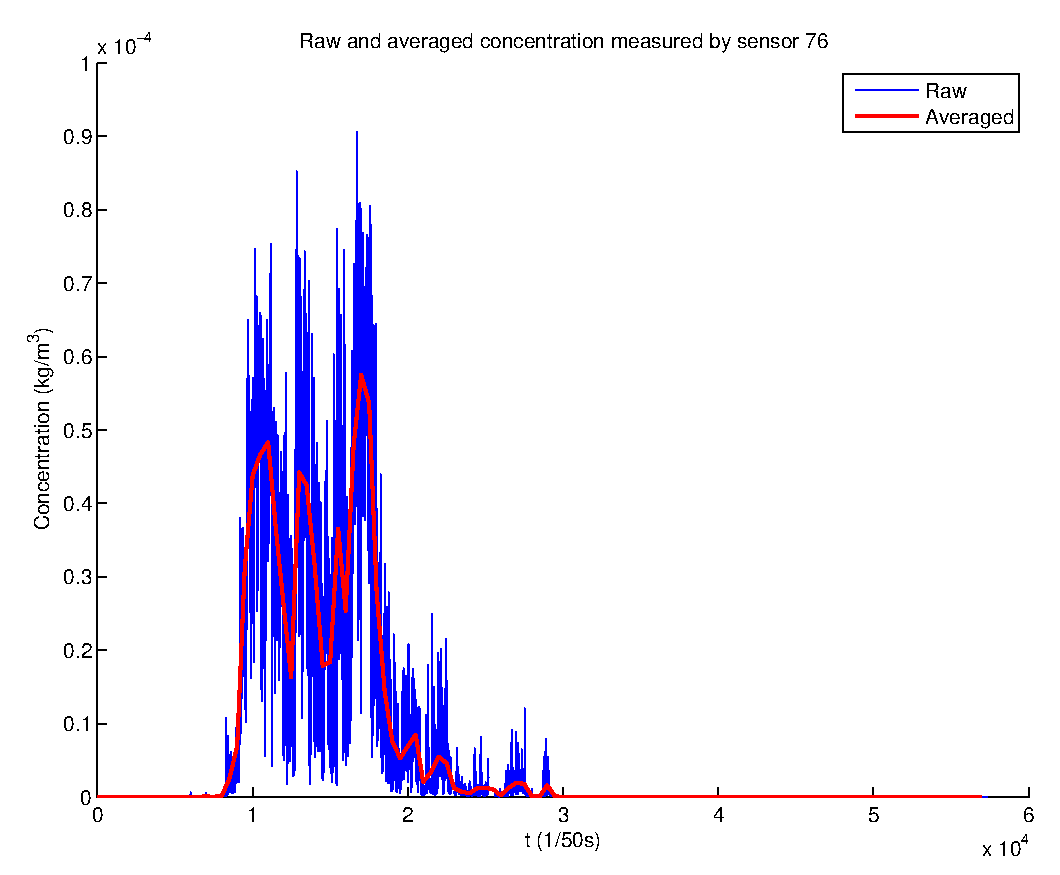
\includegraphics[scale=0.65]{moyennage_concentrations}
	\caption{Concentrations brutes (en bleu) et concentrations moyennées (en rouge) sur une fenêtre glissante de 10s. }
	\label{fig_AE_3}
\end{figure}


L'expérience FFT07 étant un outil de validation, le domaine d'étude comprend beaucoup plus de capteurs que dans un cas standard, où le domaine est moins instrumenté. Afin d'envisager un cas réaliste tout en conservant une quantité suffisante de données d'observation à traiter, nous avons choisi de limiter le nombre de capteurs \NdPA{exploités} à 25 (voir figure \ref{fig_AE_4}).

\begin{figure}[h!]
	\centering
	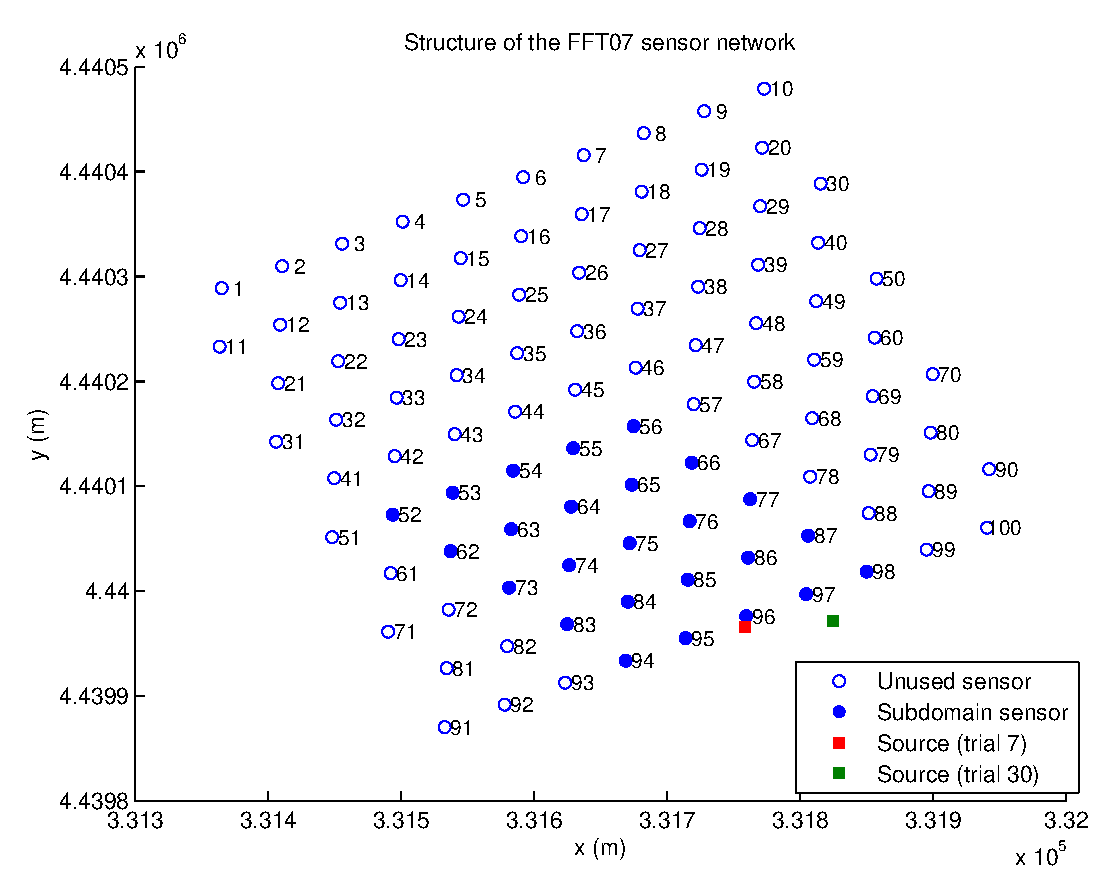
\includegraphics[scale=0.65]{FFT07_capteurs}
	\caption{Choix du sous-réseau de 25 capteurs utilisé dans notre étude.}
	\label{fig_AE_4}
\end{figure}

Dans notre cas, nous travaillons avec les configurations issues des \textit{trials} 7 et 30 \NdPA{dont les données nous sont disponibles}: 
\begin{itemize}
	\item Dans un premier temps, nous simulons à l'aide d'un modèle de dispersion les concentrations mesurées aux capteurs pour chaque \textit{trial}, afin d'exclure toute source d'erreur pouvant être causée par les différents facteurs instrumentaux.
	\item Nous confrontons ensuite l'algorithme de reconstruction du terme source aux mesures réelles des capteurs, afin de vérifier si l'estimation reste suffisamment précise par rapport au cas purement synthétique.
\end{itemize}



\section{Formulation bayésienne du problème STE}

\subsection{Modèle de données et vraisemblance}

Nous considérons ici une source localisée en un point $\PosSource = (x_s, y_s, z_s)$ de l'espace et caractérisée par un profil de rejet $\VecQSource$. Pour les besoins de la modélisation, ce dernier est discrétisé en $T_s$ échéances d'émission $t'_1, \cdots, t'_{T_s}$, l'intervalle entre deux échéances consécutives demeurant strictement identique. On peut ainsi définir $\VecQSource$ comme une succession de paliers d'émissions constantes, le débit de la source ne variant pas entre deux instants d'émission consécutifs $t'_n$ et $t'_{n+1}$.\\


On suppose que les observations sont définies par des mesures de concentration en un nombre fini de points $ \PosCapteur^{(1)}, \cdots, \PosCapteur^{(N_c)}$ du domaine, qui constituent les positions d'un réseau de $N_c$ capteurs. On considère que les capteurs et la source se situent à la même hauteur, ce qui permet de n'étudier la position de la source que sur deux dimensions, autrement dit écrire $\PosSource = (x_s, y_s)$. Les mesures fournies par ces capteurs sont données suivant une discrétisation temporelle donnée, chaque capteur délivrant ainsi une valeur de concentration à chacun des instants d'observation $t_1, \cdots, t_{T_c}$.




 La concentration $\obs_{i,j}$ fournie par le $i$-ème capteur à la position $\PosCapteur^{(i)}$ et à l'échéance d'observation $t_j$ est alors modélisée par l'équation suivante: 
 
\begin{equation}
\obs_{i,j} = \sum\limits_{n=1}^{T_s}q(t'_n)\MatC_{i,j}(\PosSource, t'_n) + \varepsilon_{i,j}
\label{eq_AE_2}
\end{equation}

Le premier terme de l'équation \eqref{eq_AE_2} représente à la concentration moyenne obtenue par la superposition des $T_s$ rejets aux  différents temps d'émission $\left\{t'_n\right\}_{1\leq n \leq T_s}$et pondérés par les quantités émises $\left\{q(t'_n)\right\}_{1 \leq n \leq T_s}$ associées. Ainsi, $\MatC_{i,j}(\PosSource, t'_n)$ désigne la concentration moyenne observée par le $i$-ème capteur à la position $\PosCapteur^{(i)}$ et à l'échéance d'observation $t_j$ pour un rejet unitaire  émis à l'instant $t'_n$ par une source située à la position $\PosSource$. Enfin, $\varepsilon_{i,j}$ représente le terme regroupant toutes les sources d'erreur présentées au paragraphe §\ref{ss_erreurs}.\\

Il est possible de réécrire l'équation \eqref{eq_AE_2} sous la forme matricielle suivante:

\begin{equation}
\VecObs = \MatC(\PosSource)\VecQSource + \VecErreur
\label{eq_AE_3}
\end{equation}
qui n'est autre que l'équivalent de l'équation \eqref{eq_relation_SR_non_parametrique}. $\VecObs \in \mathbb{R}^{N_cT_c}$ est un vecteur où toutes les observations de concentration sont concaténées sous la forme suivante : 

\begin{equation}
\VecObs = \left(\obs_{1,1}, \obs_{1,2}, \cdots, \obs_{1,T_c}, \obs_{2,1}, \cdots, \cdots, \obs_{N_c,T_c}\right)^T
\label{eq_AE_3_plus}
\end{equation}

$\VecErreur \in \mathbb{R}^{N_cT_c}$ est un vecteur d'erreur qui suit, comme présenté à l'équation \eqref{eq_bruit_obs}, une loi normale centrée de matrice de covariance $\MatR \in \mathbb{R}^{N_cT_c \times N_cT_c}$. De plus, on considère que ce vecteur de bruit affecte les observations de façon indépendante et identiquement distribuée (i.i.d.): par conséquent, la matrice $\MatR$ est diagonale: 


\begin{equation}
	\NdFS{
		\MatR = \varObs \MatId_{N_c T_c}
		}
\end{equation}

Le terme $\MatC(\PosSource) \in \mathbb{R}^{N_cT_c \times T_s}$ est la matrice source-récepteur suivante:

\begin{equation}
\MatC(\PosSource) = 
\begin{pmatrix}
\MatC_{1,1}(\PosSource, t'_1) & \MatC_{1,1}(\PosSource, t'_2)  & \cdots & \MatC_{1,}(\PosSource, t'_{T_s}) \\ 
\MatC_{1,2}(\PosSource, t'_1) & \MatC_{1,2}(\PosSource, t'_2)  & \cdots & \MatC_{1,2}(\PosSource, t'_{T_s}) \\
\vdots & \vdots &  & \vdots \\
\MatC_{1,T_c}(\PosSource, t'_1) & \MatC_{1,T_c}(\PosSource, t'_2)  & \cdots & \MatC_{1,T_c}(\PosSource, t'_{T_s}) \\
\MatC_{2,1}(\PosSource, t'_1) & \MatC_{2,1}(\PosSource, t'_2)  & \cdots & \MatC_{2,1}(\PosSource, t'_{T_s}) \\
\vdots & \vdots &  & \vdots \\
\vdots & \vdots &  & \vdots \\
\MatC_{N_c,T_c}(\PosSource,  t'_1) & \MatC_{N_c,T_c}(\PosSource,  t'_2)  & \cdots & \MatC_{N_c,T_c}(\PosSource,  t'_{T_s}) \\
\end{pmatrix}
\label{eq_AE_4}
\end{equation}

Si on note $\VecThetaMaj = (\PosSource, \VecQSource)$ le vecteur des paramètres caractérisant le terme source, la règle de Bayes permet \NdPA{de définir} la loi a posteriori de $\VecThetaMaj$ : 

\begin{equation}
p(\VecThetaMaj | \VecObs) = \dfrac{p(\VecObs | \VecThetaMaj)p(\VecThetaMaj)}{p(\VecObs)}
\label{eq_AE_1}
\end{equation}

Comme expliqué au paragraphe \ref{paragraphe_paradigme_bayesien}, on cherche à estimer cette loi a posteriori à un facteur multiplicatif près, l'équation \eqref{eq_AE_1} devient alors:

\begin{equation}
\NdFS{
p(\VecThetaMaj | \VecObs) \propto p(\VecObs | \VecThetaMaj)p(\VecThetaMaj)
}
\label{eq_AE_1_prop}
\end{equation}

Comme \NdPA{le vecteur d'erreur est supposé gaussien centré}, on peut alors définir la vraisemblance des observations $\VecObs$ sachant un terme source donné $\VecThetaMaj$:

\begin{equation}
p(\VecObs | \VecThetaMaj) = \prod\limits_{i=1}^{N_c} \prod\limits_{j=1}^{T_c}\mathcal{N}\left(\obs_{i,j} \middle\vert \MatC_{i,j}(\PosSource)\VecQSource, \varObs\right)
\label{eq_AE_5}
\end{equation}

\subsection{Choix des lois a priori}

\subsubsection{Position de la source}

On considère que la source est forcément contenue dans les limites du domaine spatial $\mathcal{D}$ considéré, mais qu'elle peut se situer en n'importe quel point de ce domaine. En termes probabilistes, cela se traduit par une loi a priori uniforme sur la position $\PosSource$ de la source:

\begin{equation}
p(\PosSource) = \mathcal{U}_\mathcal{D}(\PosSource)
\label{eq_AE_7}
\end{equation}


\subsubsection{Profil d'émission}

Comme expliqué dans \cite{Winiarek2011}, la pratique la plus courante consiste à choisir un a priori gaussien pour le vecteur $\VecQSource$, qui s'écrit alors:

\begin{equation}
p(\VecQSource) = \mathcal{N}\left(\VecQSource \middle \vert \VecMeanQ, \MatCovQ\right)
\label{eq_AE_8}
\end{equation}

Dans \cite{Bocquet2008}, il est expliqué que l'hypothèse gaussienne sur $\VecQSource$ entraîne potentiellement des incohérences physiques telles que des valeurs d'émissions négatives. Cependant, une telle hypothèse demeure fréquemment utilisée dans la littérature, et conduit à des résultats satisfaisants (voir par exemple \cite{Issartel2003}) ainsi qu'une meilleure flexibilité quant à la quantification des connaissances a priori sur le type de rejet étudié. Par exemple, si on sait d'avance que le rejet se fait à un débit relativement faible, alors il est possible d'ajuster les valeurs de la diagonale de la matrice de covariance en y mettant des quantités faibles. \\

Il est toutefois possible d'atténuer les effets indésirables de l'hypothèse gaussienne sans avoir à changer la nature de la loi de probabilité a priori de $\VecQSource$, nous verrons comment cela est possible dans le prochain paragraphe.


\section{Marginalisation du profil d'émission}

\subsection{Principe}
La vraisemblance $p(\VecObs|\VecThetaMaj)$ présentée à l'équation \eqref{eq_AE_5} est fortement non-linéaire, et la complexité de sa formulation rend impossible le calcul analytique de la loi a posteriori $p(\VecThetaMaj | \VecObs)$. Afin de contourner ce problème, une solution consiste à exprimer cette loi a posteriori en fonction des différentes \textit{lois a posteriori marginales} dont elle dépend. \\

Par définition, la loi a posteriori $p(\VecThetaMaj|\VecObs)$ peut s'exprimer en fonction de la loi jointe de $\VecThetaMaj$ et $\VecObs$:

\begin{equation}
p(\VecThetaMaj|\VecObs) = p(\PosSource, \VecQSource | \VecObs) = \dfrac{p(\PosSource, \VecQSource, \VecObs)}{p(\VecObs)}
\label{eq_conditionalite}
\end{equation}

En appliquant la règle du conditionnement en chaîne, ou \textit{chain rule}\footnote{La \textit{chain rule} permet d'exprimer une loi jointe sous la forme d'un produit de lois conditionnelles. Si on considère les $n$ variables aléatoires $X_1, \dots, X_n$, alors on a $p(X_1, \dots, X_n) = p(X_n|X_1, \dots, X_{n-1})p(X_{n-1}|X_1, \dots, X_{n-2})\dots p(X_2|X_1)p(X_1)$.}, sur le numérateur, on arrive à l'expression suivante:
\begin{equation}
p(\PosSource, \VecQSource | \VecObs) = p(\VecQSource | \PosSource, \VecObs)p(\PosSource | \VecObs)
\label{eq_AE_9}
\end{equation}
où $p(\VecQSource | \PosSource, \VecObs)$ et $p(\PosSource | \VecObs)$ sont \NdFS{les lois a posteriori respectives du profil d'émission conditionnellement à la position de la source}. \\

\subsection{A priori gaussien et solution analytique}


\NdFS{
	Etant donnés les paramètres $\VecMeanQ$ et $\MatSigma_q$ définis à l'équation \eqref{eq_AE_8} et la formulation du modèle de l'équation \eqref{eq_AE_3}  il est possible de réécrire la vraisemblance sous la forme suivante:
	
	\begin{equation}
		p(\VecObs | \VecQSource, \PosSource) = \mathcal{N}(\VecObs | \MatC(\PosSource)\VecMeanQ, \MatC(\PosSource)\MatSigma_q\MatC(\PosSource)^T + \MatR)
		\label{eq_lk_gaussian}
	\end{equation}
	
	La loi a priori de $\VecQSource$ ainsi que la vraisemblance de l'équation \eqref{eq_lk_gaussian} suivant toutes deux des lois normales, alors la loi a posteriori marginale de $\VecQSource$ suit également une loi normale de moyenne $\PostMeanQ$ et de matrice de covariance $\PostCovQ$, dont les valeurs sont obtenues par les formules empiriques: 
	 \begin{equation}
	 \begin{split}
	 \PostMeanQ & = \VecMeanQ + \MatK(\VecObs - \MatC(\PosSource)\VecMeanQ) \\
	 \PostCovQ & = \MatCovQ - \MatK\MatC(\PosSource)\MatCovQ
	 \end{split}
	 \label{eq_filtre_kalman_statique}
	 \end{equation}
	  où $\MatK$ est définie par:
	  
	  \begin{equation}
	  \MatK = \MatCovQ\MatC(\PosSource)^T(\MatC(\PosSource)\MatCovQ\MatC(\PosSource)^T + \MatR)^{-1}
	  \end{equation}
	
	}
  Les paramètres $\PostMeanQ$ et $\PostCovQ$ sont ainsi obtenus de façon analytique (i.e. sans approximation) par les équations \eqref{eq_filtre_kalman_statique}. 

\subsection{Contrainte de positivité}

Dans le but d'assurer la positivité des valeurs d'émission de la source, une contrainte peut être appliquée sur les résultats de l'équation \eqref{eq_filtre_kalman_statique}, inspirée par les travaux de \cite{Simon2010}. Il s'agit d'utiliser une méthode permettant de restreindre les valeurs d'un vecteur d'état à un intervalle borné ou semi-borné prédéfini: pour cela, la densité de probabilité de ce vecteur d'état est tronquée suivant la contrainte que l'on cherche à appliquer. \\

Le processus de troncature est ainsi appliqué de façon séquentielle sur chaque composante de $\VecQSource$: on travaille ainsi à tronquer $T_s$ densités de loi univariées. Le détail de cette démarche est décrit par l'algorithme \ref{algo_PCO}, qui permet d'approximer la loi a posteriori marginale de $\VecQSource$ par : 

\begin{equation}
p^c(\VecQSource | \PosSource, \VecObs) = \mathcal{N}(\VecQSource | \PostMeanQ^c, \PostCovQ^c)
\label{eq_AE_16}
\end{equation}

\begin{algorithm}
\begin{algorithmic}
	\State \textbf{Entrées}: $\PostMeanQ$ et $\PostCovQ$
	\State Initialisation: $\PostMeanQ^c=\PostMeanQ$ et $\PostCovQ^c=\PostCovQ$
	\For{$i=1:T_s$}
		\State ${\bm \gamma}_i=\begin{bmatrix}{\bf 0}_{1\times (i-1)} & 1  & {\bf 0}_{1\times (T_s-i)}\end{bmatrix}^T$
		\State Calculer ${\bm W}_i$ et ${\bm T}_i$ par la réduction de Jordan de $\PostCovQ^c$, i.e. ${\bm T}_i {\bm W}_i {\bm T}_i^T=\PostCovQ^c$
		\State Calculer ${\bm S}_i$ par l'orthogonalisation de Gram-Schmidt pour obtenir la matrice orthogonale ${\bm S}_i$ telle que $${\bm S}_i {\bm W}_i^{1/2} {\bm T}_i^T {\bm \gamma}_i=\begin{bmatrix}
		({\bm \gamma}_i^T \PostCovQ^c {\bm \gamma}_i)^{1/2} & 0 & \cdots & 0 
		\end{bmatrix} $$
		 $c_i=-\dfrac{{\bm \gamma}_i^T \PostMeanQ^c}{({\bm \gamma}_i^T \PostCovQ^c {\bm \gamma}_i)^{1/2}}$
		 \State $\mu_i=\dfrac{\phi(c_i)}{1-\Phi(c_i)}$ avec $\phi(\cdot)$ la densité de la loi normale centrée réduite, et $\Phi(\cdot)$ la fonction de répartition de la loi normale centreé réduite.
		 \State $\sigma^2_i=1-\mu_i(\mu_i-c_i)$
		 \State ${\bm z}_i=\begin{bmatrix}\mu_i & 0 & \cdots & 0 \end{bmatrix}^T$
		 \State ${\bm D}_i=\text{diag}(\sigma^2_i,1,\ldots,1)$
		\State Calculer les paramètres de la densité tronquée:
		\State \begin{align*}
		\begin{split}
		\PostMeanQ^c&={\bm T}_i {\bm W}_i^{1/2} {\bm S}_i ^T{\bm z}_i + \PostMeanQ^c\\
		\PostCovQ^c&={\bm T}_i {\bm W}_i^{1/2} {\bm S}_i^T {\bm D}_i  {\bm S}_i {\bm W}_i^{1/2} {\bm T}_i ^T \\
		\end{split}
		\end{align*}
	\EndFor
	\State \textbf{Sorties}: $\PostMeanQ^c$ et $\PostCovQ^c$
	\end{algorithmic}
	\caption{Contrainte de positivité sur $\VecQSource$ par troncature de la densité de $p(\VecQSource | \PosSource, \VecObs)$}
	\label{algo_PCO}
\end{algorithm}

Notons qu'une telle procédure permet également d'optimiser le calcul de la vraisemblance marginale de la localisation de la source $p(\VecObs | \PosSource)$: celle-ci peut alors se calculer par le même procédé que celui employé dans l'équation \eqref{eq_AE_9}, et devient alors:

\begin{equation}
p^c(\VecObs | \PosSource) = \dfrac{p(\VecObs | \VecQSource, \PosSource)p(\VecQSource)}{p^c(\VecQSource | \PosSource, \VecObs)}
\label{eq_AE_17}
\end{equation}


 \begin{figure}[h!]
 	\centering
 	\begin{subfigure}[t]{0.5\textwidth}
 		\centering
		\includegraphics[width=1\textwidth]{ConstrainedFigure1.eps}
		\caption{}
 		\label{fig_AE_2_a}
 	\end{subfigure}%
 	\begin{subfigure}[t]{0.5\textwidth}
 		\centering
		\includegraphics[width=1\textwidth]{ConstrainedFigure2.eps}
		\caption{}
 		\label{fig_AE_2_b}
 	\end{subfigure}
 	\begin{subfigure}[t]{0.5\textwidth}
 		\centering
 		\includegraphics[width=1\textwidth]{ConstrainedFigure3.eps}
 		\caption{}
 		\label{fig_AE_2_c}
 	\end{subfigure} 

 	\caption{Illustration de l'application de la contrainte de positivité (en noir) sur les paramètres d'une distribution gaussienne bivariée (en rouge) dans trois cas distincts: sans corrélation (\ref{fig_AE_2_a}), avec corrélation négative (\ref{fig_AE_2_b}) et avec corrélation positive (\ref{fig_AE_2_c}).}
 	 \label{fig_AE_2}	
 \end{figure}

La figure \ref{fig_AE_2} résume bien le fonctionnement de l'algorithme \ref{algo_PCO}: la zone en noir représente la version tronquée aux valeurs positives de la distribution initiale (en rouge). 

\section{Localisation de la source avec l'algorithme AMIS}

Il s'agit ici d'étudier la loi a posteriori marginale $p(\PosSource | \VecObs)$ de la position de la source. Contrairement au profil d'émission, il est \NdFS{impossible} d'obtenir une solution analytique pour caractériser cette distribution. Par conséquent, \NdFS{l'idée est d'utiliser les méthodes de simulation stochastique afin d'}approximer la distribution $p(\PosSource | \VecObs)$. \\

\subsection{Principe}

Nous appliquons l'algorithme AMIS décrit dans le chapitre 2 afin de localiser la source. Pour cela, on va ainsi construire une procédure itérative basée sur l'algorithme \ref{algo_AMIS} afin de créer sur $K$ itérations et en générant $N_p$ particules par itération un échantillon de $KN_p$ particules \NdFS{$\left\{\PosSource_k^{(i)}\right\}_{0\leq k \leq K}^{1\leq i \leq N_p}$} dont la distribution approxime celle de la loi marginale a posteriori \NdFS{$p(\PosSource | \VecObs)$} de la position de la source.\\

Dans un cadre bayésien, la loi cible recherchée peut alors s'écrire à une constante multiplicative près, suivant la relation de proportionnalité suivante:

\begin{equation}
\NdFS{
p(\PosSource | \VecObs) \propto p(\VecObs | \PosSource)p(\PosSource)
\label{eq_AE_20}
}
\end{equation}

La fonction de vraisemblance \NdFS{$p(\VecObs | \PosSource)$} est définie par l'équation \eqref{eq_AE_5} (ou \eqref{eq_AE_17} si on choisit d'appliquer la contrainte de positivité), et la loi a priori \NdFS{$p(\PosSource)$} par l'équation \eqref{eq_AE_7}. L'équation \eqref{eq_AE_20} permet ainsi d'évaluer la loi cible toute particule \NdFS{$\PosSource$} échantillonnée depuis la loi de proposition courante, afin de calculer les poids d'importance \NdPA{associés}. La structure globale de la démarche est décrite par la figure \ref{schema_amis}.\\

%\begin{figure}[h!]
%	\centering
%	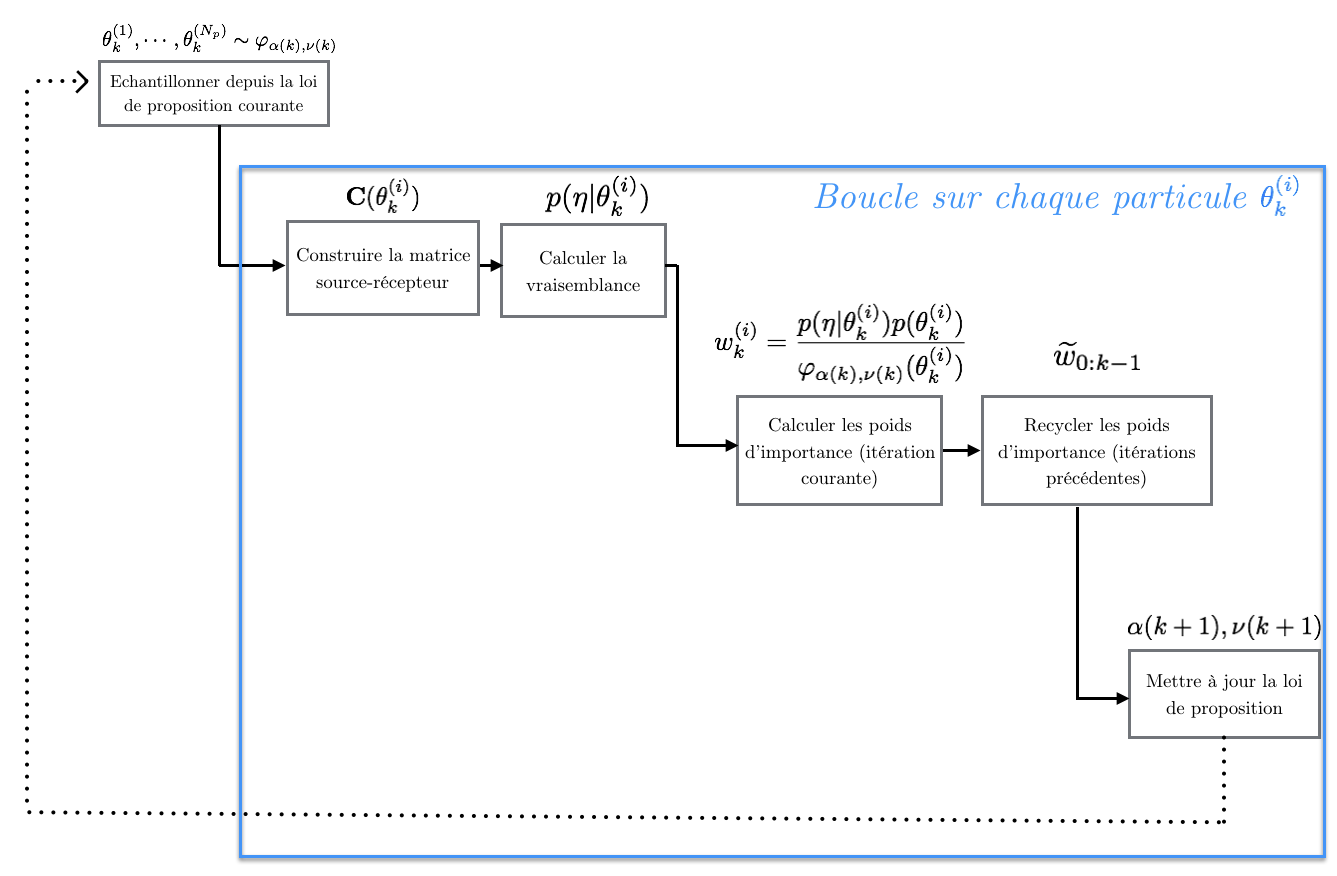
\includegraphics[width=1\textwidth]{schema_amis_capture}

%\end{figure}
\begin{figure} 
		\centering
        \begin{tikzpicture}[retour/.style={->,>=stealth’,thick,dashed}]
        \node[draw, text width = 7cm, align=center] (step_1) at (0,0) {Echantillonner $\PosSource_k^{(1)}, \dots, \PosSource_k^{(N_p)}$  depuis la loi de proposition courante $\varphi_{\alpha(k), \nu(k)}$};
        \node[draw, text width = 7cm, align=center] (step_2) at (0,-1.75) {Construire les matrices source-récepteur $\MatC(\PosSource_k^{(1)}), \dots, \MatC(\PosSource_k^{(N_p)})$ avec $N_p$ \\appels au modèle de dispersion direct};
        \node[draw, text width = 7cm, align=center] (step_3) at (0,-3.5) {Calculer les vraisemblances \\ $p(\VecObs | \PosSource_k^{(1)}), \dots, p(\VecObs | \PosSource_k^{(N_p)})$};
        \node[draw, text width = 7cm, align=center] (step_4) at (0,-6.5) {Pour chaque $i \in \{1, \cdots, N_p\}$, calculer les poids d'importance \\ $ w_k^{(i)} = \dfrac{p(\VecObs | \PosSource_k^{(i)})p(\PosSource_k^{(i)})}{\varphi_{\alpha(k), \nu(k)}(\PosSource_k^{(i)})}$ \\et normaliser: \\$\widetilde{w}_k^{(i)} = \dfrac{w_k^{(i)}}{\sum\limits_{j=1}^{N_p} w_k^{(j)}}$};
        \node[draw, text width = 7cm, align=center] (step_5) at (0,-9.75) {Recycler les poids d'importance des itérations précédentes \\ $\widetilde{w}_l^{(1)}, \dots, \widetilde{w}_l^{(N_p)}$ avec $l \in \{0, \dots, k-1\}$}; 
        \node[draw, text width = 7cm, align=center] (step_6) at (0,-12) {En utilisant $\PosSource_l^{(1)}, \dots, \PosSource_l^{(N_p)}$ et $\widetilde{w}_l^{(1)}, \dots, \widetilde{w}_l^{(N_p)}$ avec $l \in \{0, \dots, k\}$, générer les nouveaux paramètres \\ $\alpha(k+1)$ et $\nu(k+1)$ de la loi de proposition };
        %\draw[retour] (step_6)--(step_1);
        \draw[->,>=latex] (step_1) -- (step_2);
        \draw[->,>=latex] (step_2) -- (step_3);
        \draw[->,>=latex] (step_3) -- (step_4);
        \draw[->,>=latex] (step_4) -- (step_5);
        \draw[->,>=latex] (step_5) -- (step_6);
        \end{tikzpicture}
        \caption{Diagramme de fonctionnement de l'algorithme AMIS sur la $k$-ième itération pour la localisation de la source.}
        \label{schema_amis}
 \end{figure}

\subsection{Choix de la loi de proposition}

L'algorithme AMIS requiert une loi de proposition paramétrique qui soit suffisamment flexible pour:
\NdFS{
	\begin{itemize}
		\item pouvoir s'adapter de façon à être capable d'approximer correctement la loi cible une fois ses paramètres ajustés,
		\item effectuer simplement l'opération d'adaptation des paramètres. Sur ce point, le choix d'une mixture de gaussiennes telle que présentée dans \cite{Cappe2008} est cohérent, car les formules de mise à jour sont directement disponibles via l'algorithme EM.
	\end{itemize}

On définit donc la loi de proposition comme} une mixture de $D$ distribution gaussiennes bivariées:

\begin{equation}
\varphi_{(\alpha,\nu)}(\NdFS{\PosSource}) = \sum\limits_{d=1}^D \alpha_d \varphi_d(\NdFS{\PosSource} | \nu_d)
\label{eq_AE_21}
\end{equation}
où les $\alpha_d$ sont les facteurs d'influence de chacune des composantes de la mixture, et $\nu_d$ représente le vecteur des paramètres de la $d$-ième composante, telle que : 
\begin{equation}
\varphi_d(\NdFS{\PosSource} | \nu_d) = \mathcal{N}(\NdFS{\PosSource} | \VecMu_d, \MatSigma_d)
\label{eq_AE_21_bis}
\end{equation}
avec $\VecMu_d \in \mathbb{R}^2$ et $\MatSigma_d \in \mathbb{R}^{2\times2}$.

 \begin{figure}[h!]
 	\centering
 	\begin{subfigure}[t]{0.5\textwidth}
 		\centering
 		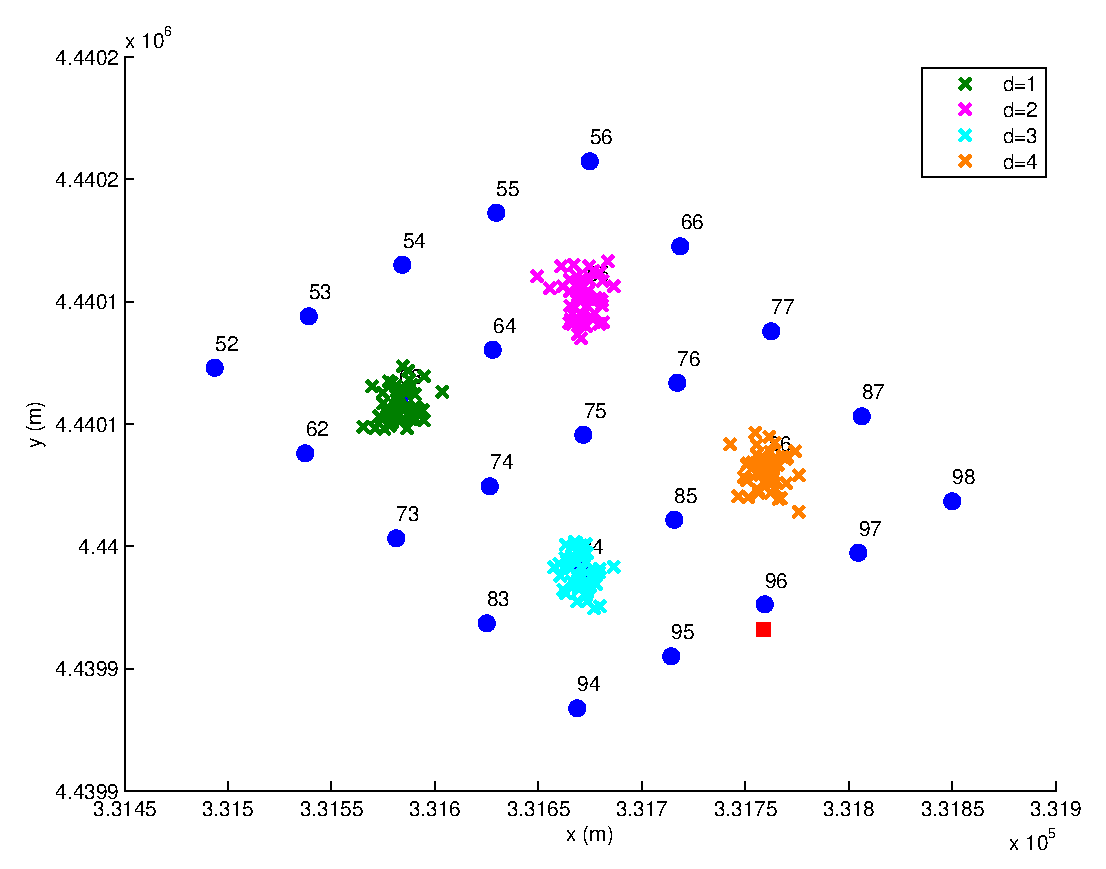
\includegraphics[width=1\textwidth]{init_amis_bad.eps}
 		\caption{$\MatSigma_d = 
 			\begin{pmatrix}
 			50 & 0 \\
 			0 & 50
 			\end{pmatrix}$}
 		\label{init_amis_bad}
 	\end{subfigure}%
 	\begin{subfigure}[t]{0.5\textwidth}
 		\centering
 		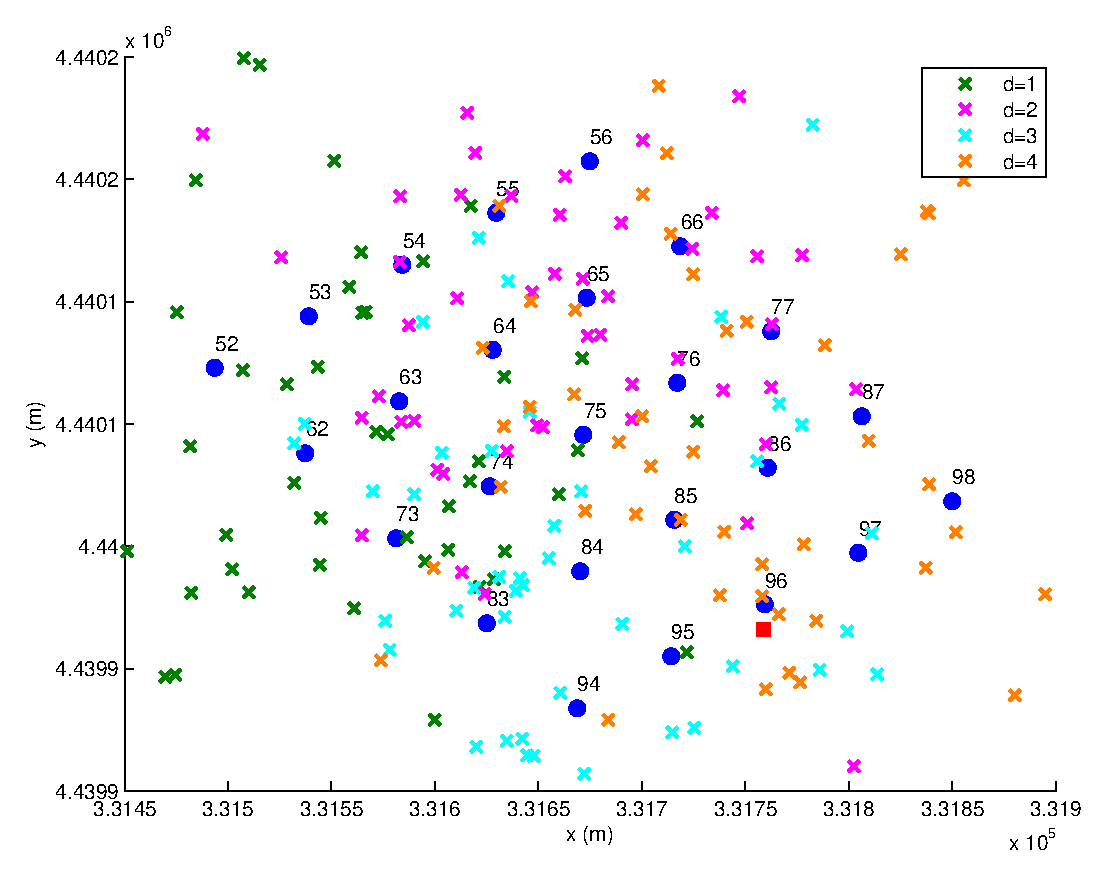
\includegraphics[width=1\textwidth]{init_amis_good.eps}
 		\caption{$\MatSigma_d = 
 			\begin{pmatrix}
 			5000 & 0 \\
 			0 & 5000
 			\end{pmatrix}$}
 		\label{init_amis_good}
 	\end{subfigure}
 	\caption{Exemples d'initialisation de l'AMIS avec $D=4$ composantes pour la loi de proposition: un bon choix des $\MatSigma_d$ permet un tirage homogène sur le domaine (\ref{init_amis_good}) tandis qu'une covariance trop faible ne permettra pas d'explorer tout le domaine (\ref{init_amis_bad}).}
 	 \label{fig_init_amis}	
 \end{figure}
 
  Le choix des paramètres initiaux permet de régler la surface couverte par chacune des composantes afin d'obtenir une répartition relativement homogène des particules, illustrant une absence de connaissance a priori sur une localisation potentielle de la source (voir figure \ref{fig_init_amis}). \\
  
  En pratique, nous avons:
  
  \begin{enumerate}
  	\item divisé le domaine en quatre quadrants de surface égale, 
  	\item  placé les moyennes $\VecMu_d$ sur le centre de chacun des quadrants,
  	\item réglé les matrices de covariance $\MatSigma_d$ de façon à ce que chacune des composantes de la mixture fournisse des échantillons couvrant toute la surface de son quadrant.\\
  \end{enumerate}
  
 \NdFS{Si une information a priori est disponible (par exemple, des zones particulières du domaine à exclure ou à favoriser), les paramètres $\alpha_d, \VecMu_d$ et $\MatSigma_d$ avec $d \in \{1,\dots,D\}$ peuvent être préalablement ajustés afin d'orienter en conséquence l'échantillonnage des particules dès la première itération. Un exemple de ce type d'initialisation est présenté au Chapitre 4.
 	
 	Une fois l'algorithme lancé, à chaque itération, ces paramètres  sont mis à jour grâce aux formules des équations \eqref{eq_maj_gaussien}.}\\


\section{Description du modèle de dispersion à bouffées gaussiennes}

Une fois la loi de proposition initialisée, on peut exécuter la boucle itérative de l'algorithme AMIS telle que décrite à l'algorithme \ref{algo_AMIS}. Dans cet algorithme, le calcul de la loi de vraisemblance telle que décrite à l'équation \eqref{eq_AE_5} requiert l'exécution d'un modèle de dispersion pour obtenir $\MatC(\PosSource)$. Ici, nous choisissons d'utiliser un modèle \textit{à boufféees gaussiennes}, ou \textit{Gaussian Puff Model} (GPM). Nous expliquons brièvement dans la suite de ce paragraphe les principes de base régissant ce type de modèles.\\

Les modèles gaussiens permettent de représenter la dispersion à petite échelle autour d'une source. Pour cela, une formulation analytique de la concentration du polluant est calculée suivant plusieurs hypothèses permettant une mise en oeuvre simple et peu coûteuse en temps de calcul. Il existe deux types différents de modèles gaussiens:\\

\begin{itemize}
	\item les modèles dits \textit{de panache} (ou \textit{Gaussian plume}), où la dispersion est modélisée dans des conditions météorologiques supposées uniformes et stationnaires. Le panache émis par la source est alors modélisé par une distribution de type gaussienne dans deux directions: celle orthogonale au vent, et la direction verticale (voir figure \ref{gaussian_plume}).
	\item les modèles dits \textit{à bouffées} (ou \textit{Gaussian puff}), modélisant une série d'émissions instantanées représentées par des bouffées à distribution gaussienne dans les trois directions de l'espace, et dont les centres sont transportés par un champ de vent qui peut  être non-uniforme et non-stationnaire. La globalité du rejet à un instant donné est ainsi illustrée par la somme des différentes bouffées émises par la source (voir figure \ref{gaussian_puff}). C'est ce type de modèle que nous utilisons dans l'étude de cas sur FFT07.
\end{itemize}

 \begin{figure}[h!]
 	\label{fig_gaussian_models}	
 	\centering
 	\begin{subfigure}[t]{0.5\textwidth}
 		\centering
 		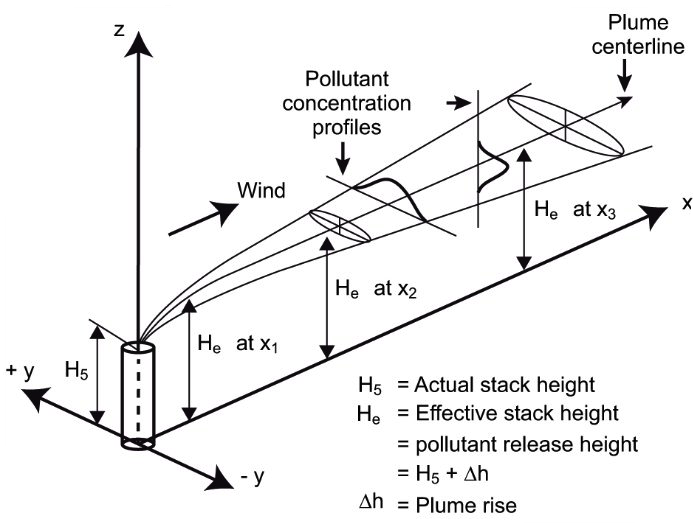
\includegraphics[width=1\textwidth]{gaussian_plume.jpg}
 		\caption{Modèle de panache gaussien \cite{Schulze1996}}
 		\label{gaussian_plume}
 	\end{subfigure}%
 	\begin{subfigure}[t]{0.5\textwidth}
 		\centering
 		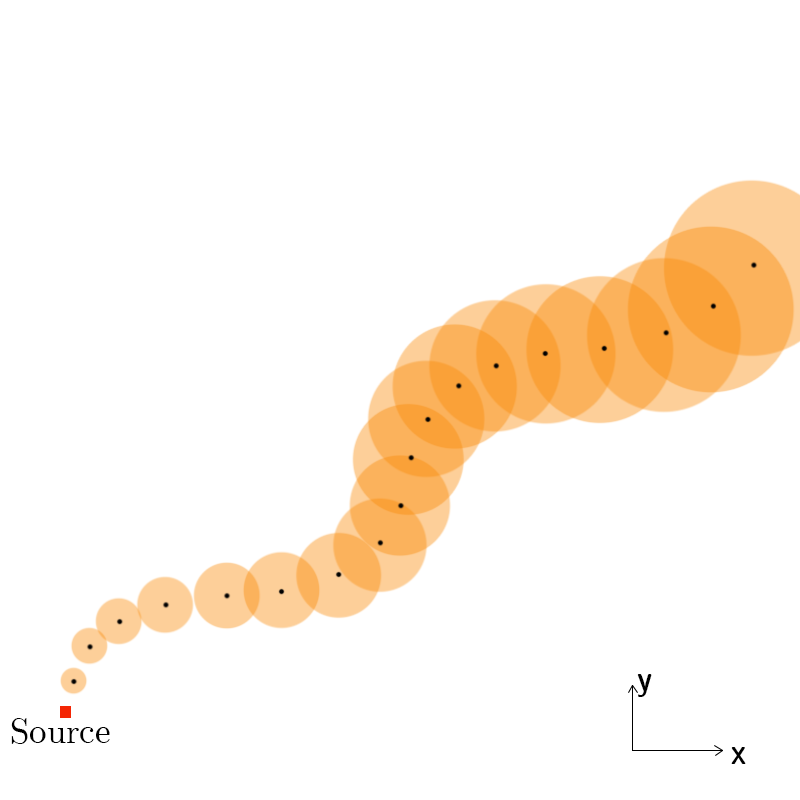
\includegraphics[width=1\textwidth]{gaussian_puff}
 		\caption{Modèle de bouffées gaussiennes}
 		\label{gaussian_puff}
 	\end{subfigure}
 	
 	\caption{Schémas de principe des modèles de dispersion gaussiens à panache (\ref{gaussian_plume}) et à bouffées (\ref{gaussian_puff})}
 \end{figure}
 
 Dans le cadre de FFT07, le choix d'un modèle à bouffées par rapport à un modèle à panache est justifié par \NdPA{le caractère instationnaire} du profil d'émission que nous cherchons à estimer. La grandeur $\VecQSource$ est en effet un vecteur, et non une valeur constante, comme c'est le cas si on appliquait un modèle de type \textit{Gaussian plume}. Cela permet également de prendre en compte les variations météorologiques telles que des changements de direction de vent. \\
 
 La concentration mesurée au $i$-ème capteur $\PosCapteur^{(i)} = (x_c^{(i)}, y_c^{(i)})$ au temps d'observation $t_j$ résultant d'une source localisée en $\PosSource$ émettant un rejet instantané à l'instant $t'_n$ est donnée par: 
 
 \begin{equation}
 \MatC_{i,j}(\PosSource, t'_n) = \dfrac{2Q_u\Delta t_p}{(2\pi)^{3/2}s_x s_y s_z}\exp\left[-\dfrac{1}{2}(\Lambda_x^2 + \Lambda_y^2)\right]
 \label{eq_AE_27}
 \end{equation}
 où:
 \begin{itemize}
 	\item $Q_u$ est la quantité unitaire de polluant émise: comme les concentrations fournies par les capteurs sont en kg/m$^3$ on a $Q_u = 1\text{kg/s}$,
 	\item $\Delta t_p$ est l'écart temporel entre l'émission de deux bouffées consécutives dans le modèle de dispersion, ici $\Delta t_p = 1$s,
 	\item $s_x, s_y, s_z$ sont les coefficients de dispersion sur les trois axes de l'espace,
 	\item les grandeurs $\Lambda_x$ et $\Lambda_y$ sont définies par : 
 	
 	\begin{equation}
 	\begin{split}
 	\Lambda_x &= \dfrac{x_c^{(i)} - \left(\PosSource + \sum\limits_{t=t'_n}^{t_j}u_x(t)\delta_w\right)}{s_x}\\
 	 	\Lambda_y &= \dfrac{y_c^{(i)} - \left(\PosSource + \sum\limits_{t=t'_n}^{t_j}v_x(t)\delta_w\right)}{s_y}
 	\end{split}
 	\end{equation}
 	$\delta_w$ est l'intervalle de temps entre deux valeurs de mesures du vent, ce dernier étant représenté par ses deux composantes $u_x$ et $v_x$.
 \end{itemize}
 
 On se place dans le cas d'une diffusion isotrope en $x$ et $y$, on a ainsi $s_x = s_y$. Les valeurs de $s_y$ et $s_z$ sont obtenues par la formule suivante : 
 
 \begin{equation}
 \begin{split}
 s_y &= a_y [d(\PosSource, \bm{x}_p)]^{b_y}\\
 s_z &= a_z [d(\PosSource, \bm{x}_p)]^{b_z}
 \end{split}
 \end{equation}
 où $a_x, a_y, b_x, b_y$ sont des coefficients empiriques qui dépendent de la classe de stabilité atmosphérique \cite{Pasquill1983} et $d(\PosSource, \bm{x}_p)$ est la distance entre la source $\PosSource$ et le centre $\bm{x}_p$ de la bouffée courante. On utilise ici la classe de Pasquill D, qui est la plus appropriée pour des conditions stables en topographie non-urbaine. 
 Comme les valeurs de la composante verticale du vent qui ont été relevées sont relativement faibles, et étant donné que les capteurs et la source se trouvent assez près du sol (2m), on ne tient pas non plus compte du terme en $z$ qui apparaît dans l'exponentielle dans la formulation générale du modèle \NdFS{à bouffées gaussiennes}.

\section{Présentation des résultats}

\subsection{Résultats obtenus avec des données simulées}
\label{par_simule}

Dans un premier temps, afin de valider la méthode, le choix est fait de se placer dans un cadre synthétique, à savoir reproduire les conditions de l'expérience FFT07 et simuler les concentrations mesurées aux capteurs grâce à l'exécution d'un modèle de dispersion, en l'occurence le modèle gaussien défini au paragraphe précédent. Ainsi, les positions des capteurs et des sources sont exactement les mêmes que celles des \textit{trials} 7 et 30 de FFT07. Les données météorologiques sont ajustées afin que les concentrations simulées soient les plus proches possibles des relevés expérimentaux, et le vent est considéré constant en direction et en vitesse. \\

L'algorithme AMIS a été exécuté sur $K = 10$ itérations, avec $N_p = 100$ particules échantillonnées par itération. \NdFS{La loi de proposition comporte $D=4$ composantes.} Les observations synthétiques ont été générées avec un ajout de bruit gaussien centré de variance $10^{-5}$ afin de simuler les différents éléments d'erreurs présents dans le cas expérimental. La variance d'observation est fixée à $\varObs = 10^{-5}$. La loi a priori de $\VecQSource$ a été choisie telle que $\VecMeanQ = 0$ et $\MatCovQ = \varQ \bm{I}$ avec $\varQ = 10^{-3}$. En pratique, diminuer $\varQ$ revient à supposer \NdFS{a priori} que la source est proche des capteurs ayant mesuré une concentration non-nulle, et à l'inverse une variance $\varQ$ élevée implique une source potentiellement plus éloignée. 
\NdPA{Les valeurs choisies} pour les différents paramètres énumérés ci-dessus sont celles ayant permis d'obtenir les résultats les plus plausibles, présentés ci-après. \\

\subsubsection{Estimation de la position}

L'algorithme a été testé avec deux positions de source différentes, correspondant respectivement aux \textit{trials} 7 et 30, leurs coordonnées (en km) sont données par : 
\begin{equation}
\begin{split}
\PosSource^{(7)} &= (331.759;4439.960) \\
\PosSource^{(30)} &= (331.825;4439.972)
\end{split}
\end{equation}

 \begin{figure}[h!]
 	\centering
 	\begin{subfigure}[t]{1\textwidth}
 		\centering
 		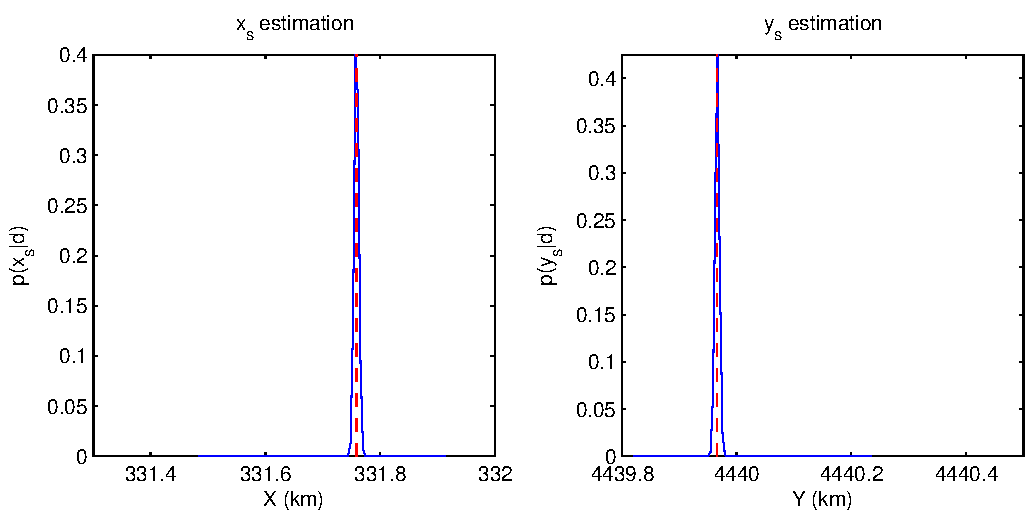
\includegraphics[width=1\textwidth]{fig_5_1}
 		\caption{Trial 7}
 		\label{fig_5_1_AE}
 	\end{subfigure}
 	\begin{subfigure}[t]{1\textwidth}
 		\centering
 		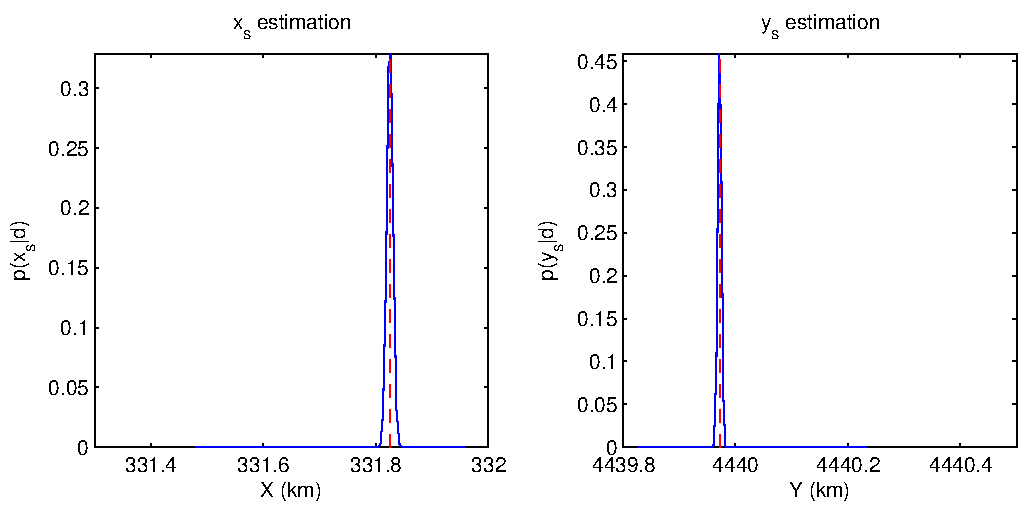
\includegraphics[width=1\textwidth]{fig_5_2}
 		\caption{Trial 30}
 		\label{fig_5_2_AE}
 	\end{subfigure}
 	\caption{Distributions a posteriori de la position de la source (en bleu) à partir de données d'observations synthétiques pour le trial 7 (\ref{fig_5_1_AE}) et le trial 30 (\ref{fig_5_2_AE}). La position réelle de la source est en pointillés rouges.}
 	\label{fig_5_AE}
 \end{figure}
 On peut voir sur la figure \ref{fig_5_AE} que l'AMIS fournit une bonne estimation de la position de la source dans chacun des \textit{trials}.\\
 
  Le fait de visualiser une distribution de probabilité permet ainsi une vision plus explicite des aspects liés aux incertitudes autour de l'estimation,  en comparaison avec des méthodes de type optimisation où seule une estimation ponctuelle est donnée.
  
  Pour obtenir les distributions présentées à la figure \ref{fig_5_AE}, \NdFS{un lissage par noyau} a été effectué afin de construire une densité de probabilité à partir d'une population statistique, en l'occurence les particules $\left\{\VecTheta_k^{(i)}\right\}_{0\leq k \leq K}^{1\leq i \leq N_p}$ associées à leurs poids d'importance respectifs $\left\{\widetilde{w}_k^{(i)}\right\}_{0\leq k \leq K}^{1\leq i \leq N_p}$. \\
  
  
  Néanmoins, il est toujours possible d'obtenir un estimateur ponctuel à partir des lois a posteriori, il suffit pour cela de calculer, \NdFS{par exemple}, le MMSE selon la formule suivante: 
  
  \begin{equation}
  \widehat{\PosSource} = \sum\limits_{k=0}^K\sum\limits_{i=1}^{N_p} \tilde{w}_k^{(i)}\VecTheta_{k}^{(i)}
  \end{equation}
  
  On arrive ainsi à un point estimé distant de moins d'un mètre par rapport à la position réelle de la source. \\

  \subsubsection{Estimation du profil de rejet}
  
  La figure \ref{fig_6_AE} illustre l'impact de l'utilisation de la contrainte de positivité pour l'estimation du profil du rejet $\VecQSource$.
  
 \begin{figure}[h!]
 	\centering
 	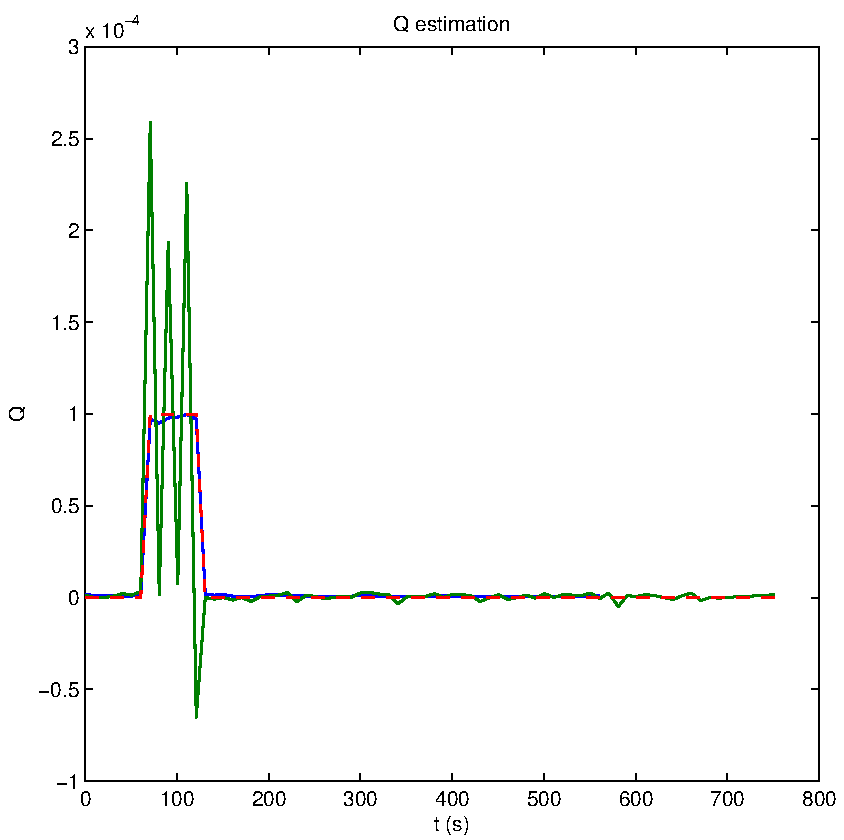
\includegraphics[width=0.5\textwidth]{fig_6}
 	\caption{Estimation de $\VecQSource$ sans (vert) et avec (bleu) application de la contrainte de positivité, comparaison avec le profil d'émission recherché (rouge).}
 	\label{fig_6_AE}
 \end{figure}
 
 L'application de la contrainte de positivité améliore le résultat de l'estimation et permet de retrouver un profil d'émission suffisamment proche de celui recherché pour avoir une bonne estimation, tant en termes d'amplitude du débit que de détection des temps d'activation et d'arrêt d'émission de la source.\\
 
 En général, du fait de sa nature potentiellement variable, le profil d'émission de la source peut prendre différents types d'allures. Nous avons ainsi modifié ce profil afin de représenter des cas non-triviaux, généré les observations correspondantes, et cherché à retrouver les caractéristiques de la source. \\
 
  \begin{figure}[h!]
  	\centering
  	\begin{subfigure}[t]{0.5\textwidth}
  		\centering
  		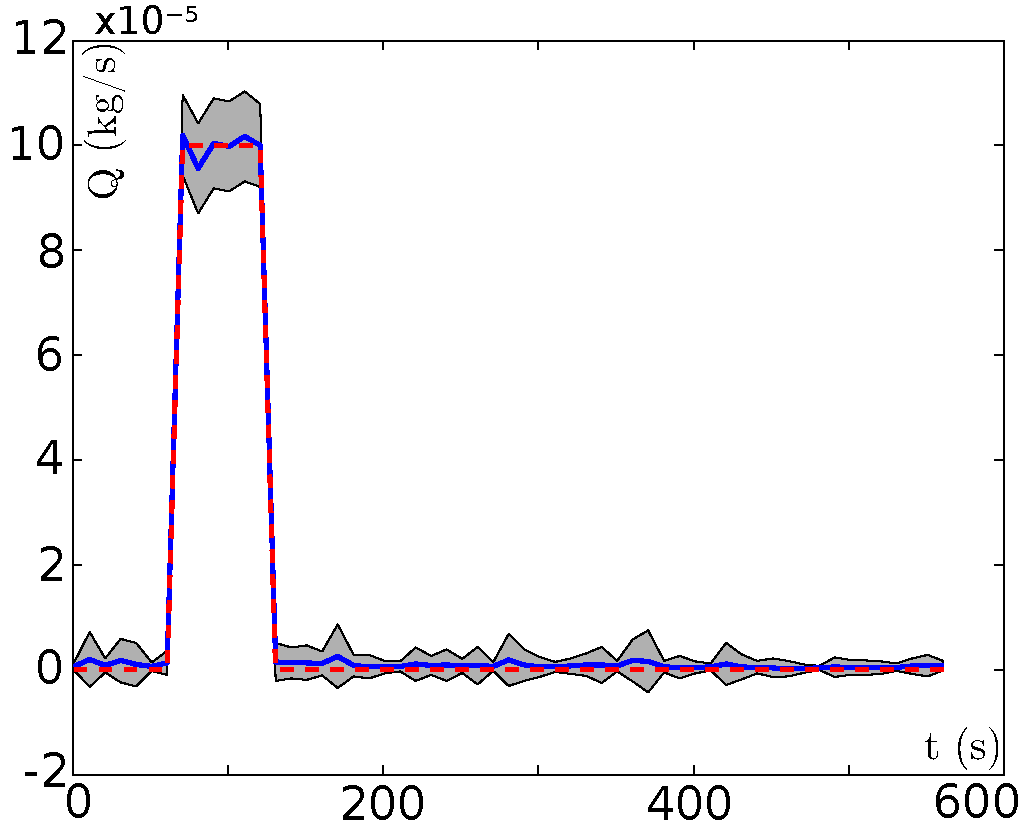
\includegraphics[width=1\textwidth]{fig_7_A}
  		\caption{}
  		\label{fig_AE_7_A}
  	\end{subfigure}%
  	\begin{subfigure}[t]{0.5\textwidth}
  		\centering
  		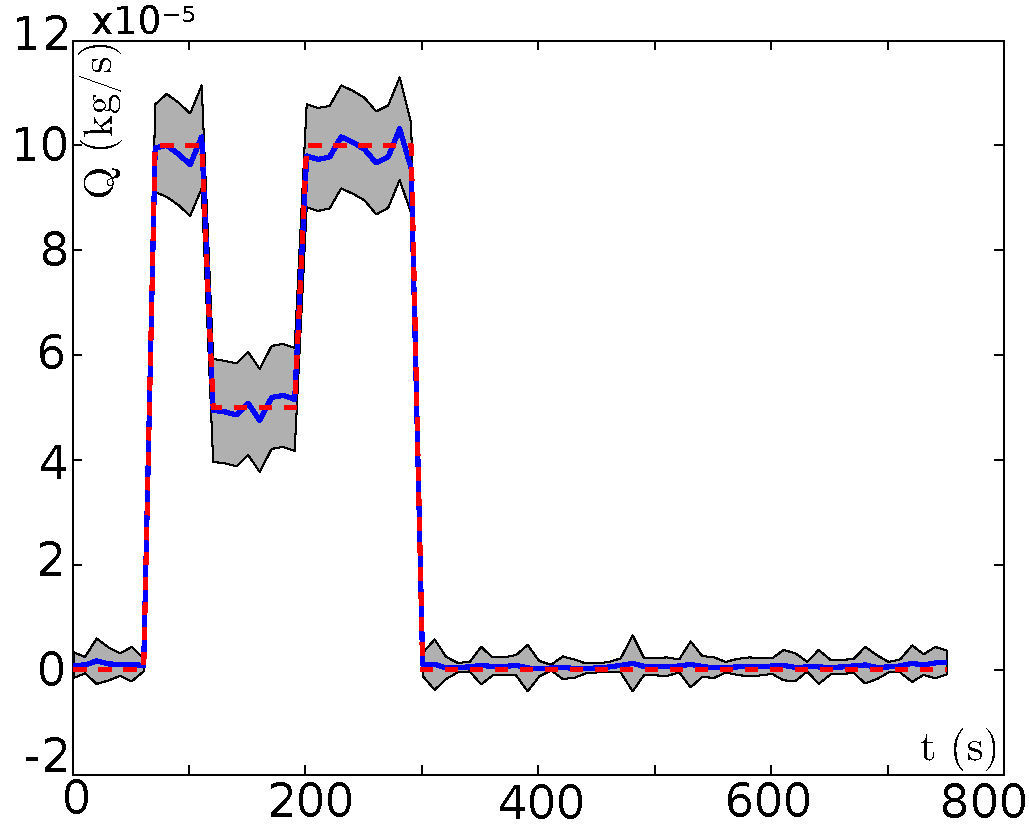
\includegraphics[width=1\textwidth]{fig_7_B}
  		\caption{}
  		\label{fig_AE_7_B}
  	\end{subfigure}
  	\begin{subfigure}[t]{0.5\textwidth}
  		\centering
  		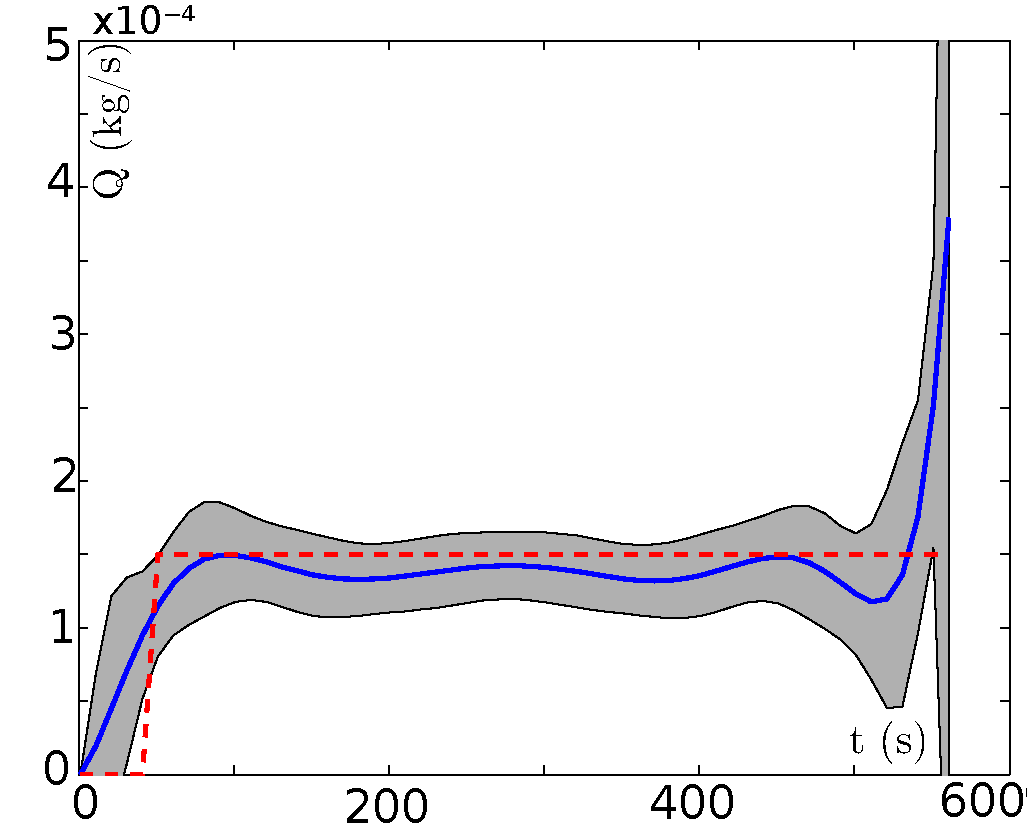
\includegraphics[width=1\textwidth]{fig_7_C}
  		\caption{}
  		\label{fig_AE_7_C}
  	\end{subfigure} 
  	
  	\caption{Simulation et résultats d'estimation pour différents profils d'émission: rejet simple (\ref{fig_AE_7_A}), rejet variable (\ref{fig_AE_7_B}), rejet continu (\ref{fig_AE_7_C}). Le profil à retrouver (en rouge) est comparé au profil estimé (en bleu) et à l'intervalle de confiance à $\pm 2 \widetilde{\sigma}_q$ (en gris).}
  	\label{fig_AE_7}	
  \end{figure}
  
  Comme présenté en figure \ref{fig_AE_7}, la méthode parvient à fournir une bonne estimation du profil de rejet dans les trois cas présentés. Sachant que l'estimation de la loi a posteriori de $\VecQSource$ consiste à estimer à la fois $\PostMeanQ$ et $\PostCovQ$, il est possible de représenter la marge d'incertitude associée à chaque valeur estimée: pour chacun des cas de la figure \ref{fig_AE_7} la valeur réelle du débit est bien incluse dans l'intervalle à $\pm 2\widetilde{\sigma}_q$, où $\widetilde{\sigma}_q^2 = \text{diag}(\PostCovQ)$. Dans le cas de la figure \ref{fig_AE_7_C}, \NdFS{on observe un effet de bord sur la fin du rejet estimé, phénomène qui est absent des autres configurations. Cela est dû au fait que l'algorithme ne dispose pas des mesures permettant de confirmer ou non les valeurs non-nulles prises par le débit estimé, ces observations étant après la limite supérieure de la fenêtre temporelle d'observation. Le problème ne se pose pas dans les configurations précédentes, car comme les concentrations mesurées sont nulles au dernier instant d'observation, l'algorithme laisse la valeur de débit estimé égale à sa moyenne a priori, à savoir 0.}
  
  
  le pic à la limite de l'intervalle d'émission est dû au fait que le rejet est plus long que la période d'observation: en l'absence d'information, l'algorithme ne peut fournir une estimation correcte, mais demeure cohérent  en augmentant fortement la taille de la marge d'incertitude, signifiant ainsi que l'information manque. \\
  
  \subsubsection{Robustesse statistique de l'estimation}
    
    L'algorithme AMIS est une procédure basée sur l'échantillonnage d'importance, qui est par nature une démarche aléatoire. Pour tenir compte de cette caractéristique dans la validation de notre méthodologie, nous avons exécuté l'AMIS sur plusieurs \textit{runs}, avec et sans application de la contrainte de positivité, et en perturbant les observations de concentrations fournies. Nous avons ensuite comparé les performances dans chacun des cas, en analysant les résultats présentés au tableau \ref{table_1_AE}. 
    
    \begin{table}[h!]
    	\centering
    	
    	\begin{tabular}{cccc}
    		
    		Contrainte de positivité & $\bar{d}(\widehat{\PosSource},\PosSource)$ (m)& $\sigma_{\widehat{x_s}}$ (m)& $\sigma_{\widehat{y_s}}$ (m)\\
    		\hline
    		OUI                   & \NdFS{$<1$}  	& 0.9        & 3.2        \\
    		NON                   & 10.44   & 0.4        & 1.0 \\      
    		\hline
    	\end{tabular}
    	\caption{Evaluation statistique des estimations sur 40 runs de l'AMIS avec et sans application de la contrainte de positivité. $\bar{d}(\widehat{\PosSource},\PosSource)$ représente la distance moyenne entre la position de source estimée par MMSE et l'emplacement réel de la source. $\sigma_{\widehat{x_s}}$ et $\sigma_{\widehat{y_s}}$ sont respectivement les moyennes des écarts-types des distributions a posteriori marginales $p(x_s | \VecObs)$ et $p(y_s | \VecObs)$. }
    	\label{table_1_AE}
    \end{table}
    
    Ces résultats confirment que l'application de la contrainte de positivité apporte en moyenne une certaine amélioration au niveau de la localisation de la source. Si on cherche à quantifier la précision de l'estimation du profil de rejet, on peut calculer l'erreur quadratique moyenne, ou \textit{mean square error} (MSE), entre la valeur estimée $\PostMeanQ$ et la valeur théorique $\VecQSource$ selon la formule suivante: 
    
    \begin{equation}
    \text{MSE}(\PostMeanQ, \VecQSource) = \dfrac{1}{T_s}\sum\limits_{n=1}^{T_s}\left(\PostMeanQ(t'_n) - \VecQSource(t'_n)\right)^2
    \label{eq_AE_31}
    \end{equation}
    
Dans le cas où on applique la contrainte de positivité, on a une erreur MSE de $1.37\times10^{-12}$, qui est une meilleure valeur que pour le cas sans contrainte, où on a une erreur MSE de $1.26\times10^{-9}$.  \\

\subsubsection{Comparaison avec le MCMC}

Nous avons ensuite cherché à comparer les performances de l'AMIS avec un autre algorithme d'inférence bayésienne couramment utilisé pour les problèmes STE, en l'occurence la méthode MCMC, présentée dans le Chapitre 2. \\

Pour cela, nous avons implémenté une algorithme de type \textit{random walk Metropolis}  avec un noyau de transition gaussien fixe, et l'intégration de la contrainte de positivité de l'algorithme \ref{algo_PCO} dans le calcul de la vraisemblance, sur 1000 itérations. Afin de tenir compte du phénomène de \textit{burn-in}, les 100 premiers états sont ignorés. \\

Un test de robustesse statistique a ensuite été effectué, en changeant de façon aléatoire le point de départ de la chaîne de Markov à chaque \textit{run} (uniformément sur le domaine). Pour la localisation de la source, l'estimateur MMSE moyen obtenu par MCMC a été comparé aux résultats de l'AMIS dans le tableau \ref{table_2_AE}. \\

    \begin{table}[h!]
    	\centering
    	
    	\begin{tabular}{cccc}
    		
    		Algorithme &\NdFS{ $\bar{d}(\widehat{\PosSource},\PosSource)$ (m)}& $\sigma_{\widehat{x_s}}$ (m)& $\sigma_{\widehat{y_s}}$ (m)\\
    		\hline
    		AMIS                   & \NdFS{$<1$}  	& 0.9        & 3.2        \\
    		MCMC                   & \NdFS{22.7}  & 130        & 95 \\      
    		\hline
    	\end{tabular}
    	\caption{Evaluation statistique des estimations sur 40 \textit{runs} de l'AMIS et du MCMC avec application de la contrainte de positivité.}
    	\label{table_2_AE}
    \end{table}
    
 Dans cette étude de cas, on remarque ainsi que les performances de l'AMIS sont meilleures en termes de précision pour localiser la source. De fait, l'approche MCMC est en partie pénalisée par l'étape d'initialisation. En effet, la convergence vers une position suffisamment proche de la vraie source est d'autant plus longue et incertaine que l'état initial de cette chaîne est éloigné de la vraie source. En ce sens, le fait de travailler sur une population de particules plutôt que sur la succession d'états séquentiels, ainsi que l'aspect adaptatif de l'AMIS lui permettent une meilleure flexibilité pour la mise à jour des paramètres de la loi de proposition, réduisant ainsi la dépendance de ses performances par rapport à l'état initial. Une alternative serait d'instancier plusieurs chaînes de Markov dont les états initiaux sont suffisamment éloignés les uns des autres pour bien couvrir le domaine, mais cela augmente la charge de calcul et les ressources requises pour l'exécution de l'algorithme. \\
 
 En plus de la précision de chacun des algorithmes, nous nous sommes également penchés sur leur vitesse de convergence. \\
 
 \begin{figure}[h!]
 	\centering
 	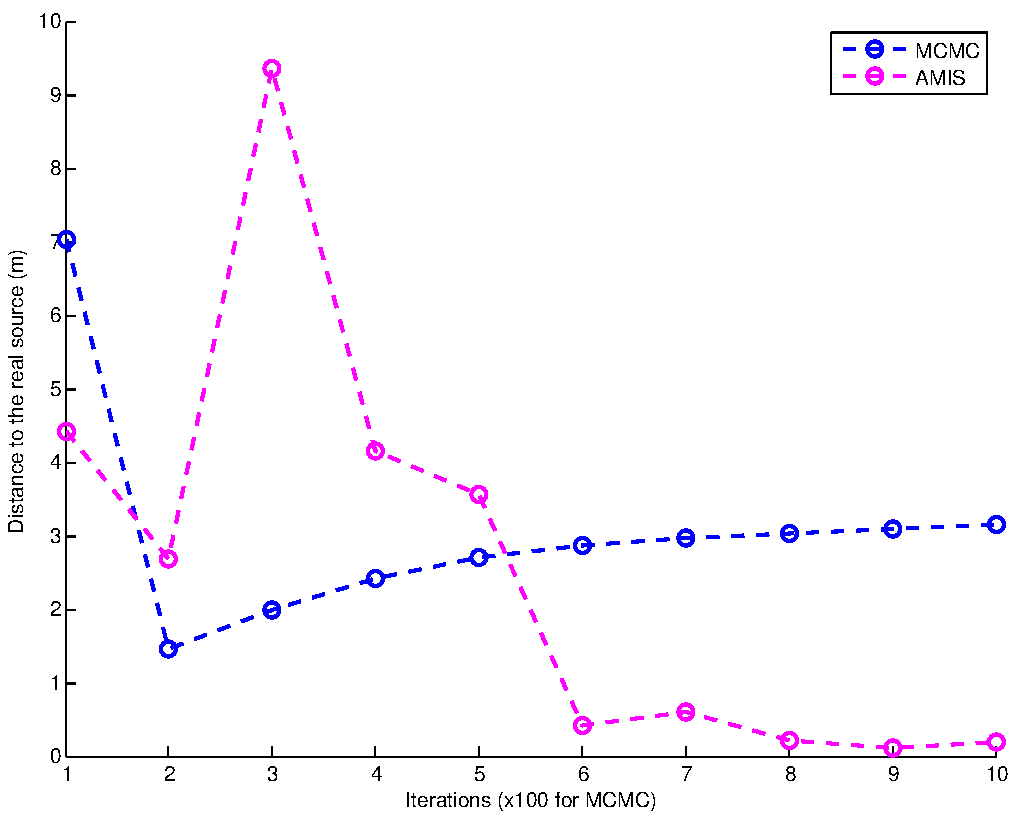
\includegraphics[width=0.7\textwidth]{fig_8}
 	\caption{Comparaison empirique de la vitesse de convergence entre MCMC (en bleu) et AMIS (en magenta)}
 	\label{fig_8_AE} 	
 \end{figure}

 Sur la figure \ref{fig_8_AE}, on utilise un critère qualitatif qui est la distance de l'estimation MMSE du lieu du rejet à une itération donnée. Les calculs ont été calibrés afin que chacun des algorithmes traite une charge équivalente de calcul. Ainsi, avec:
 \begin{itemize}
 	\item $N_p=100$ particules par itérations et $K=10$ itérations pour l'AMIS,
 	\item $1000$ itérations pour le MCMC,
 \end{itemize} 
 le nombre de calculs de la loi de vraisemblance, et par extension le nombre d'appels au modèle de dispersion, est strictement le même pour les deux algorithmes. \\
 
 Les résultats obtenus démontrent l'efficacité de l'aspect adaptatif de l'AMIS, qui lui permet d'atteindre rapidement une estimation de bonne qualité pour la localisation de la source.\\
 
 Encore une fois, dans la démarche MCMC, l'initialisation de la chaîne de Markov influe sur la vitesse de convergence, cette dernière étant d'autant plus élevée que l'état initial se situe près de la vraie source. Un autre paramètre du MCMC intervient également ici: la variance du noyau de transition. En effet, comme expliqué au Chapitre 2, si la valeur choisie pour cette variance est trop faible, même si l'initialisation place la chaîne dans une position relativement favorable, la convergence sera trop lente car le nombre d'états nécessaires pour atteindre une estimation correcte sera plus élevé. A l'inverse, il est risqué de trop augmenter la valeur de cette variance, car cela entraînerait des transitions d'amplitude trop élevée, pouvant potentiellement empêcher la convergence vers le point source recherché. L'AMIS est quant à lui plus souple dans sa démarche de transition d'une itération à l'autre, cependant il peut être également sujet à des problèmes de convergence si, par exemple, les particules échantillonnées par la loi de proposition initiale ne couvrent pas du tout la zone où se situe la vraie source, d'où l'intérêt d'une initialisation homogène telle que présentée à la figure \ref{init_amis_good}.\\
 
 \subsubsection{Effective Sample Size}
 
 Un critère spécifique aux méthodes basées sur l'échantillonnage d'importance est la représentativité de la distribution cible en fonction des particules ayant été échantillonnées afin d'approximer cette loi. Un outil permettant de quantifier cette grandeur est l'ESS, tel que présenté à l'équation \eqref{eq_def_ESS}, il permet ici en particulier de surveiller si l'AMIS est bloqué par un effet de dégénérescence des poids, ce qui se manifeste par une valeur d'ESS constamment faible. \\
 
 \begin{figure}[h!]
 	\centering
 	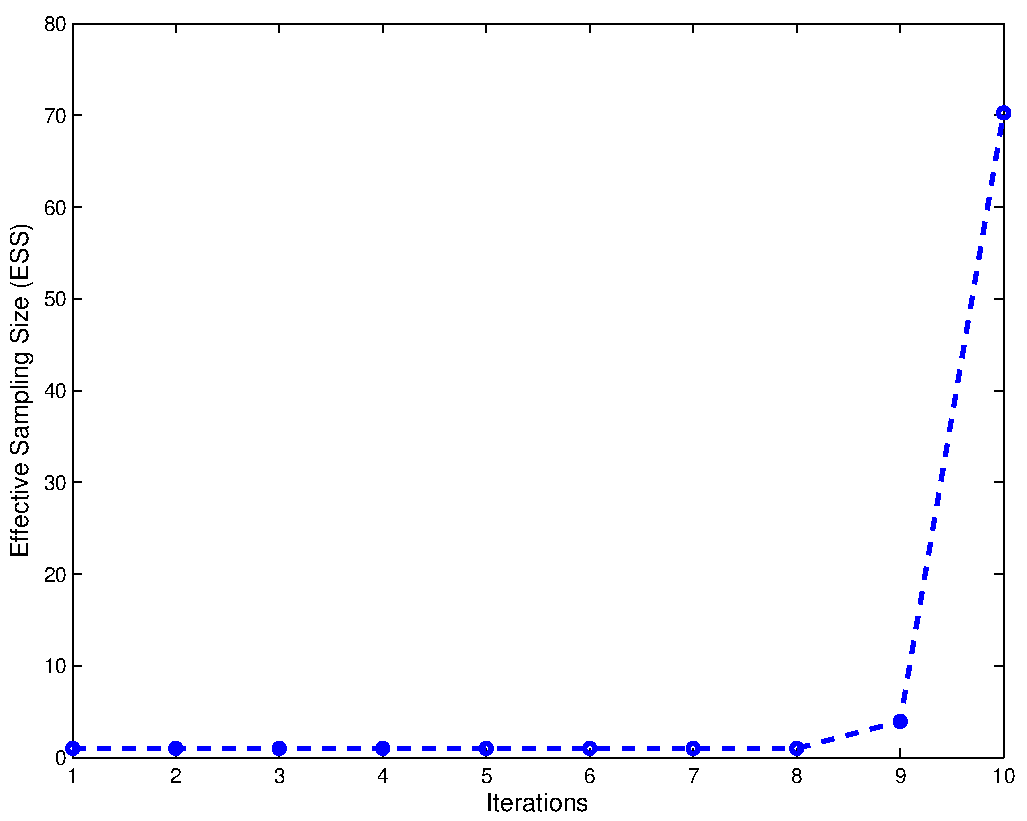
\includegraphics[width=0.7\textwidth]{fig_9}
 	\caption{Evolution de l'ESS par itération (avec $N_p=100$ particules tirées par itération)}
 	\label{fig_9_AE}
 \end{figure}
 
 On observe sur la figure \ref{fig_9_AE} que l'ESS prend un certain \NdPA{nombre d'itérations} avant d'atteindre des valeurs suffisamment élevées, néanmoins l'estimation de la position de la source devient rapidement pertinente si on se réfère à la figure \ref{fig_8_AE}. En pratique, cela illustre le fait que l'AMIS a tendance à affecter un poids relativement élevé à un nombre restreint de particules (voire à une particule unique) proches de la vraie source. 
 
 
 \subsection{Résultats obtenus avec des données expérimentales}
 
 Après un premier ensemble de tests sur données simulées, nous avons appliqué la même méthodologie en utilisant les mesures de concentrations expérimentales directement issues de l'expérience FFT07. \\
 
 \subsubsection{Traitement des données manquantes}
 
 Une première analyse des données d'observation a permis de mettre en évidence l'absence de mesures de concentrations sur certaines plages temporelles, voire sur la totalité de la fenêtre d'observation, pour plusieurs capteurs du réseau, dans les \textit{trials} 7 et 30. Ces données manquantes sont le résultat de défaillances ponctuelles des dispositifs instrumentaux au moment des essais. Nous avons ainsi eu à gérer deux types de situations:
 
 \begin{itemize}
 	\item Dans les cas où les données sont partiellement manquantes, typiquement s'il existe une quantité finie de points de mesure où les concentrations ne sont pas disponibles, alors une interpolation linéaire est faite pour remplir les valeurs manquantes à partir des concentrations disponibles.
 	\item Dans les cas où aucune concentration n'est disponible sur un capteur donné, ce dernier est écarté du réseau et n'est pas intégré au vecteur d'observations $\VecObs$. La même opération est faite si la proportion des points de mesures manquants est significativement supérieure à la quantité de mesures valables, l'opération d'interpolation étant dans ces cas-à susceptible d'introduire une information faussée.\\
 \end{itemize}
 
\subsubsection{Variabilité météorologique}

Le fait d'utiliser des données expérimentales permet également de prendre en compte la présence de variations de vitesse et de direction du vent, et voir si l'algorithme d'estimation de la source arrive à gérer une telle situation. En particulier dans le \textit{trial} 7, la direction du vent change sensiblement durant la période du rejet, comme le montre la figure \ref{fig_11_AE}.

\begin{figure}[h!]
	\centering
	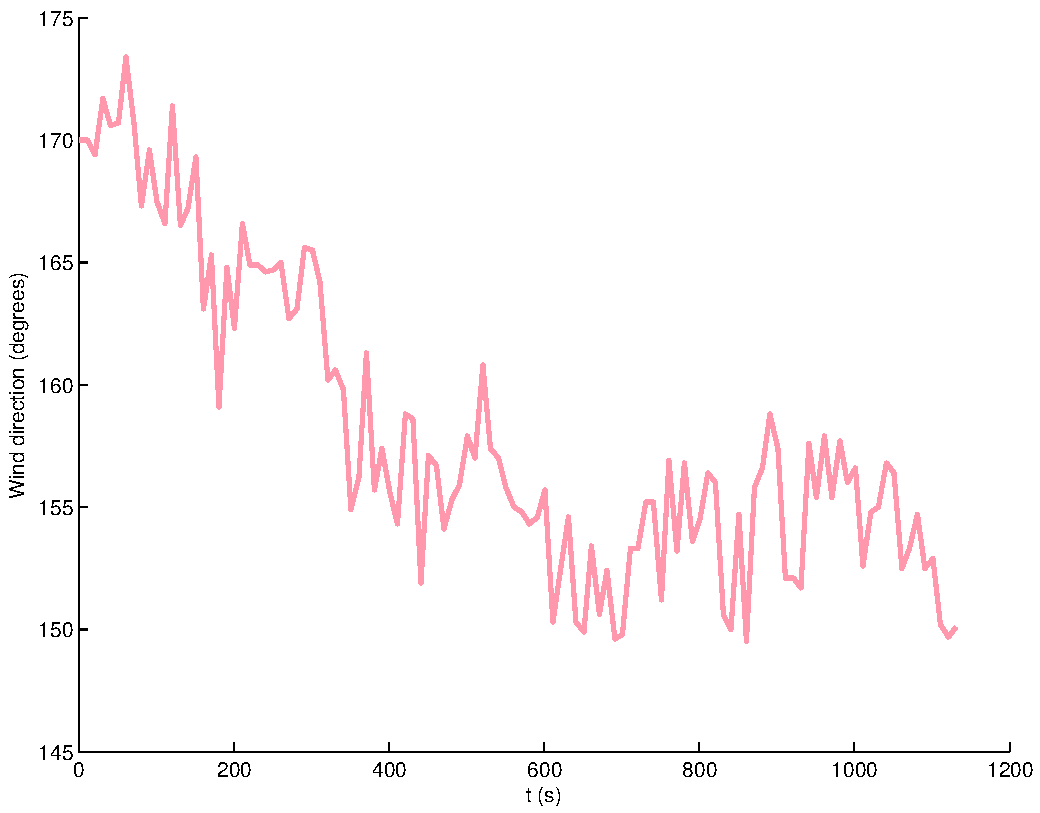
\includegraphics[width=0.7\textwidth]{fig_11}
	\caption{Direction du vent mesurée par la station météorologique la plus proche de la source (\textit{trial} 7)}
	\label{fig_11_AE}
\end{figure}

Le choix d'un modèle de dispersion à bouffées gaussiennes permet ainsi d'intégrer ces variations de vent: pour le \textit{trial} 7 nous avons donc recueilli et moyenné les mesures de vent issues des deux capteurs de vent soniques (anémomètres à ultrasons) présents sur le domaine, puis intégré les valeurs résultantes dans le modèle de dispersion. Pour le \textit{trial} 30 les variations sont beaucoup moins importantes, nous avons donc gardé l'hypothèse d'un vent stationnaire uniforme. \\

\subsubsection{Estimation de la position (\textit{trials} 7 et 30)}

De même que pour le cas synthétique, nous avons \NdFS{obtenu} par KDE les distributions a posteriori de la position de la source sur chacun des axes, et représenté les résultats pour les \textit{trials} 7 et 30 sur les figures \ref{fig_12_AE} et \ref{fig_13_AE}. Les paramètres suivants ont été utilisés:

\begin{itemize}
	\item \textit{trial} 7: $\varObs = 10^{-10}$ et $\varQ = 5\times 10^{-2}$,
	\item \textit{trial} 30: $\varObs = 5 \times 10^{-8}$ et $\varQ = 5\times 10^{-3}$.\\
\end{itemize}

\begin{figure}[h!]
	\centering
	\begin{subfigure}[t]{0.5\textwidth}
		\centering
		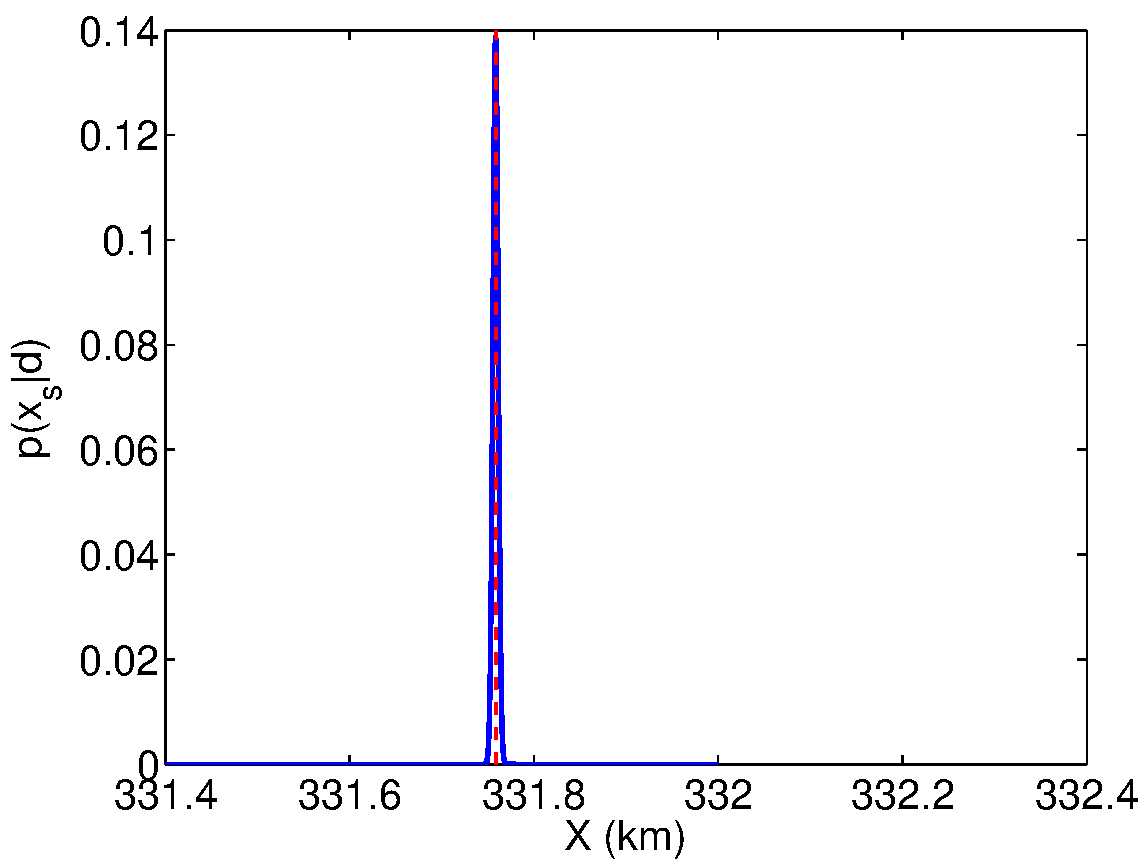
\includegraphics[width=1\textwidth]{fig_12_A}
		\caption{}
		\label{fig_12_A}
	\end{subfigure}%
	\begin{subfigure}[t]{0.5\textwidth}
		\centering
		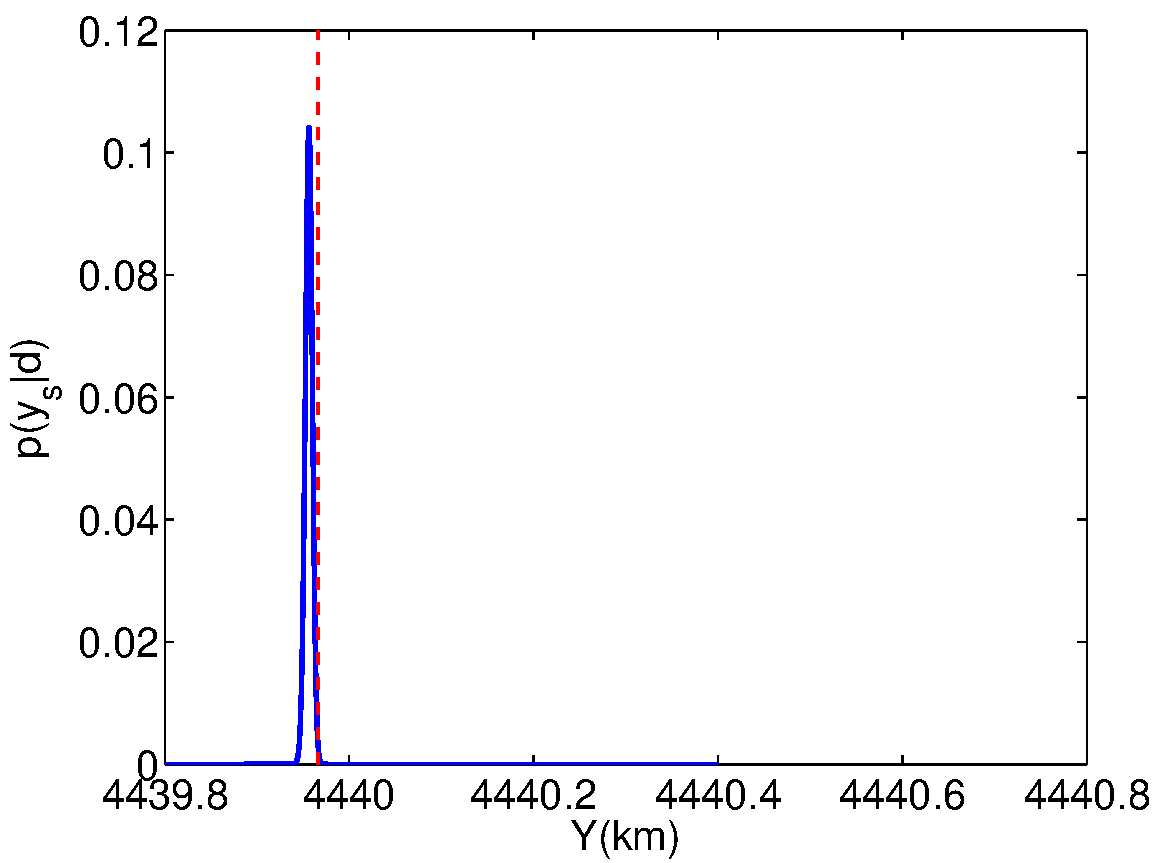
\includegraphics[width=1\textwidth]{fig_12_B}
		\caption{}
		\label{fig_12_B}
	\end{subfigure}
	\caption{Distribution a posteriori de la position de la source (en bleu) à partir des données d'observations expérimentales FFT07 pour le \textit{trial} 7. La position réelle de la source est en pointillés rouges.} 
	\label{fig_12_AE}		
\end{figure}

\begin{figure}[h!]
	\centering
	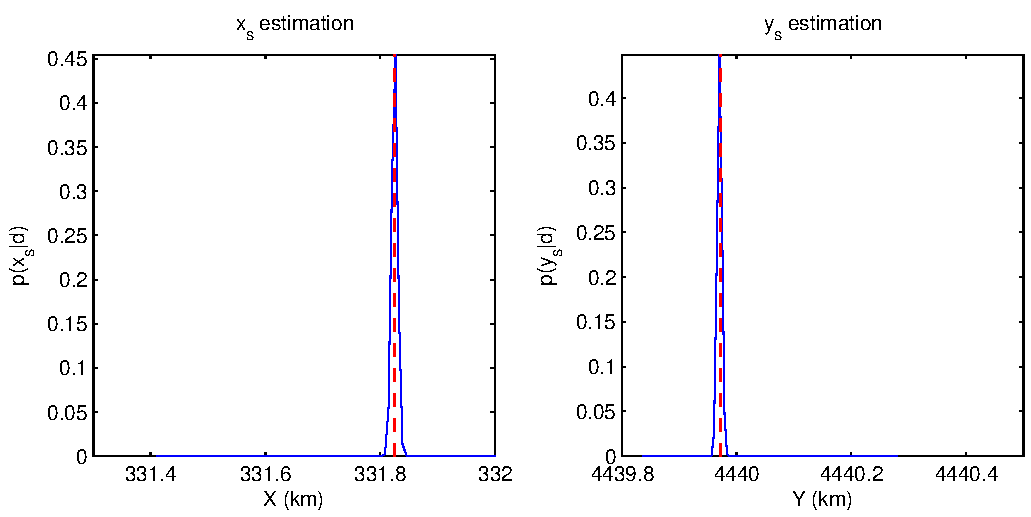
\includegraphics[width=1\textwidth]{fig_13}
	\caption{Distribution a posteriori de la position de la source (en bleu) à partir des données d'observations expérimentales FFT07 pour le \textit{trial} 30. La position réelle de la source est en pointillés rouges.}
	\label{fig_13_AE}
\end{figure}

On observe que les résultats sont presque aussi bons que dans le cas synthétique. En termes de distance de l'estimée ponctuelle MMSE par rapport à la vraie source, on reste sur des valeurs satisfaisantes de 9.8m pour le \textit{trial} 7 et 1.5m pour le \textit{trial} 30. 

\subsubsection{Comparaison avec le MCMC (\textit{trial} 7)}

Une comparaison avec le même type d'algorithme MCMC que le paragraphe §\ref{par_simule} a également été menée, en utilisant les données expérimentales du \textit{trial} 7. On remarque sur la figure \ref{fig_14_AE} que pour l'estimation de la position, les deux méthodes fournissent des résultats globalement satisfaisants. \\

\begin{figure}[h!]
	\centering
	\begin{subfigure}[t]{0.5\textwidth}
		\centering
		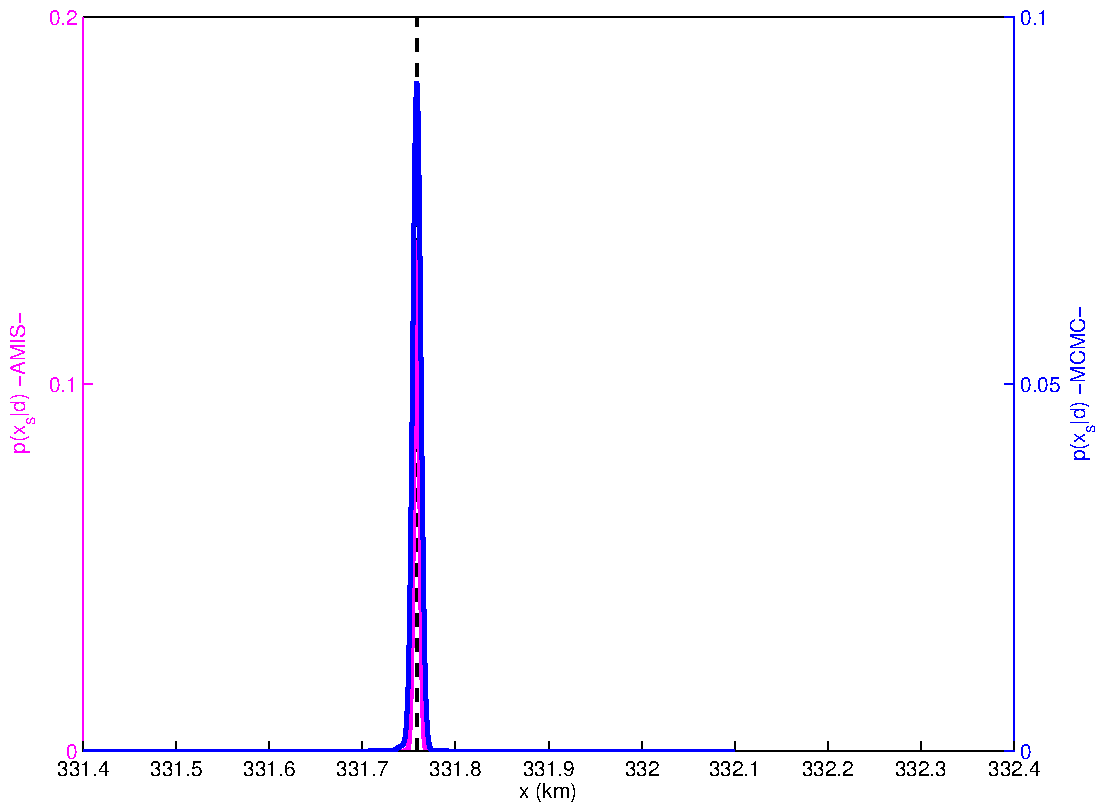
\includegraphics[width=1\textwidth]{fig_14_A}
		\caption{}
		\label{fig_14_A}
	\end{subfigure}%
	\centering
	\begin{subfigure}[t]{0.5\textwidth}
		\centering
		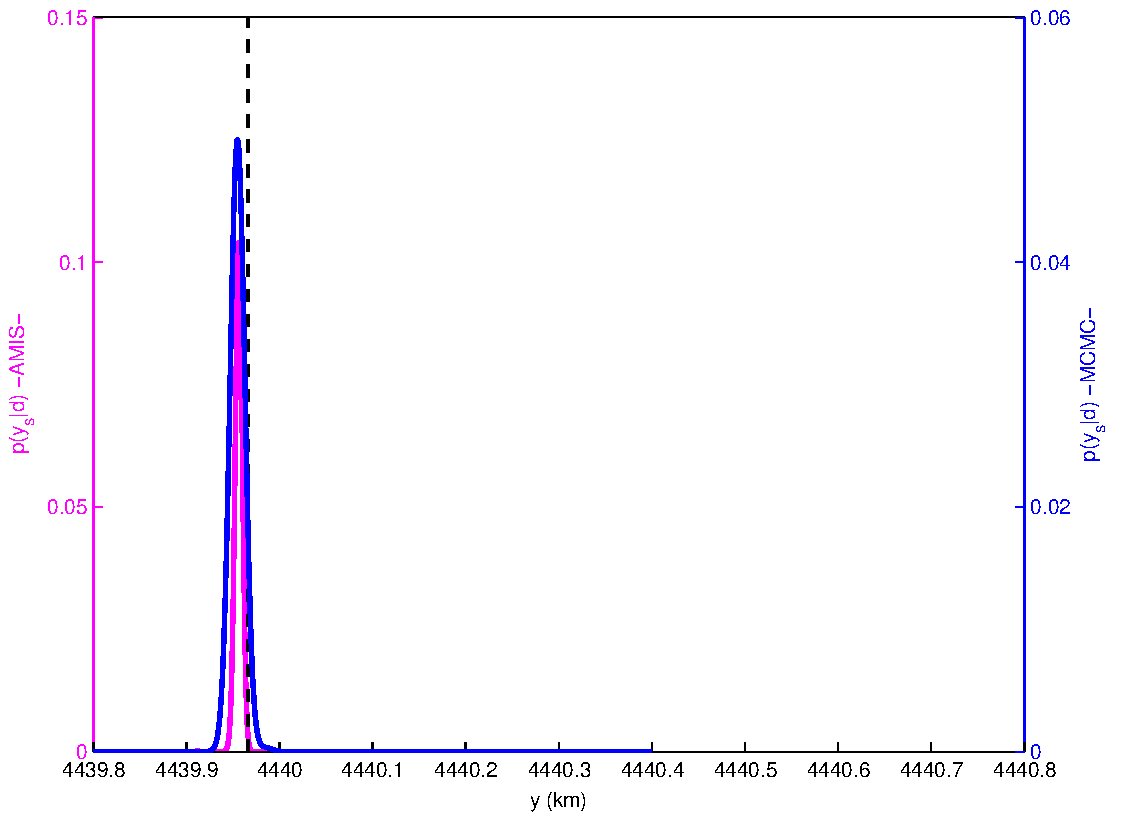
\includegraphics[width=1\textwidth]{fig_14_B}
		\caption{}
		\label{fig_14_B}
	\end{subfigure}
	\caption{Comparaison de l'estimation de la position de la source du \textit{trial} 7 avec des observations réelles en utilisant AMIS (en magenta) et MCMC (en bleu). La position réelle de la source est en pointillés noirs.}
	\label{fig_14_AE} 
\end{figure}

La comparaison a aussi été faite avec les résultats d'estimation du profil de rejet, comme illustré en figure \ref{fig_15_AE}. Les résultats ont été moyennés sur des fenêtres d'1 minute afin de lisser l'allure du débit.

 On note que les premières valeurs non-nulles du débit estimé apparaissent plus tôt qu'attendu, et avec des amplitudes plus importantes. Cela est en partie causé par le fait que l'estimée ponctuelle de la source a été située  en amont de la position réelle, ce qui a forcé l'algorithme à produire un débit plus important pour ajuster en conséquence les concentrations résultantes au niveau des capteurs, et à avancer l'instant de "démarrage" du rejet. Ce phénomène est un peu plus marqué dans le cas du MCMC (\ref{fig_15_B}).

\begin{figure}[h!]
	\centering
	\begin{subfigure}[t]{0.5\textwidth}
		\centering
		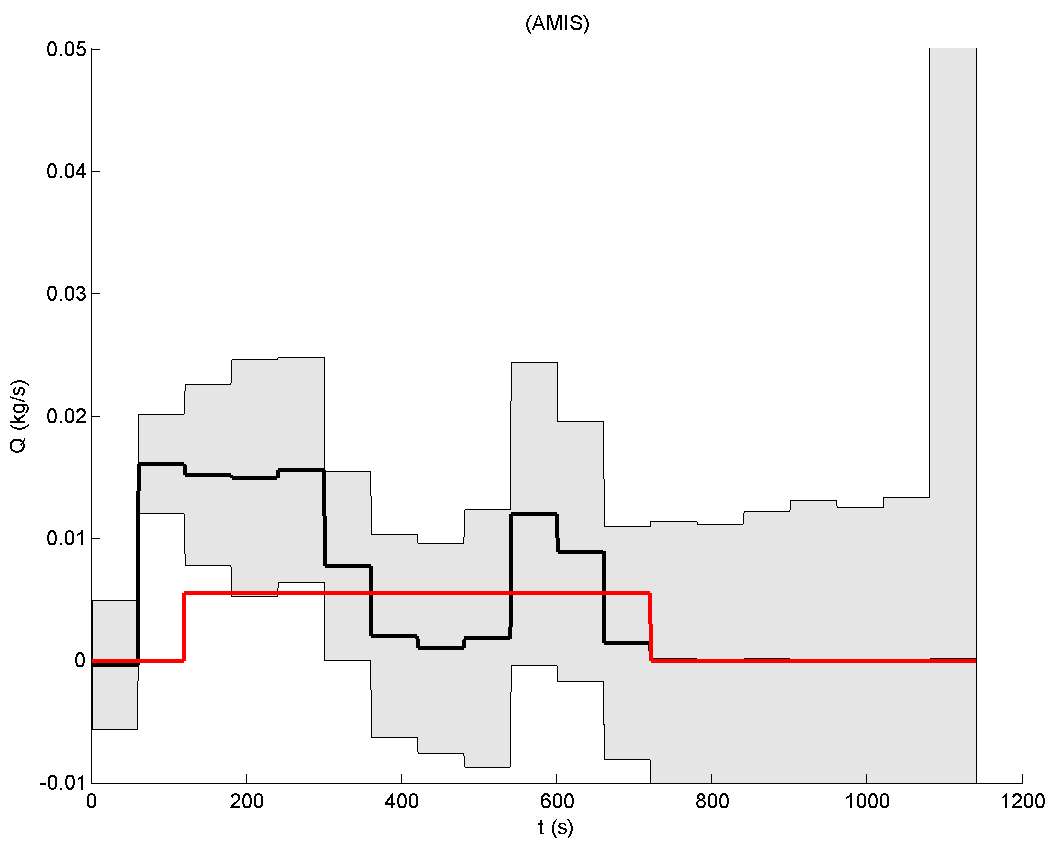
\includegraphics[width=1\textwidth]{fig_15_A}
		\caption{AMIS}
		\label{fig_15_A}
	\end{subfigure}%
	\centering
	\begin{subfigure}[t]{0.5\textwidth}
		\centering
		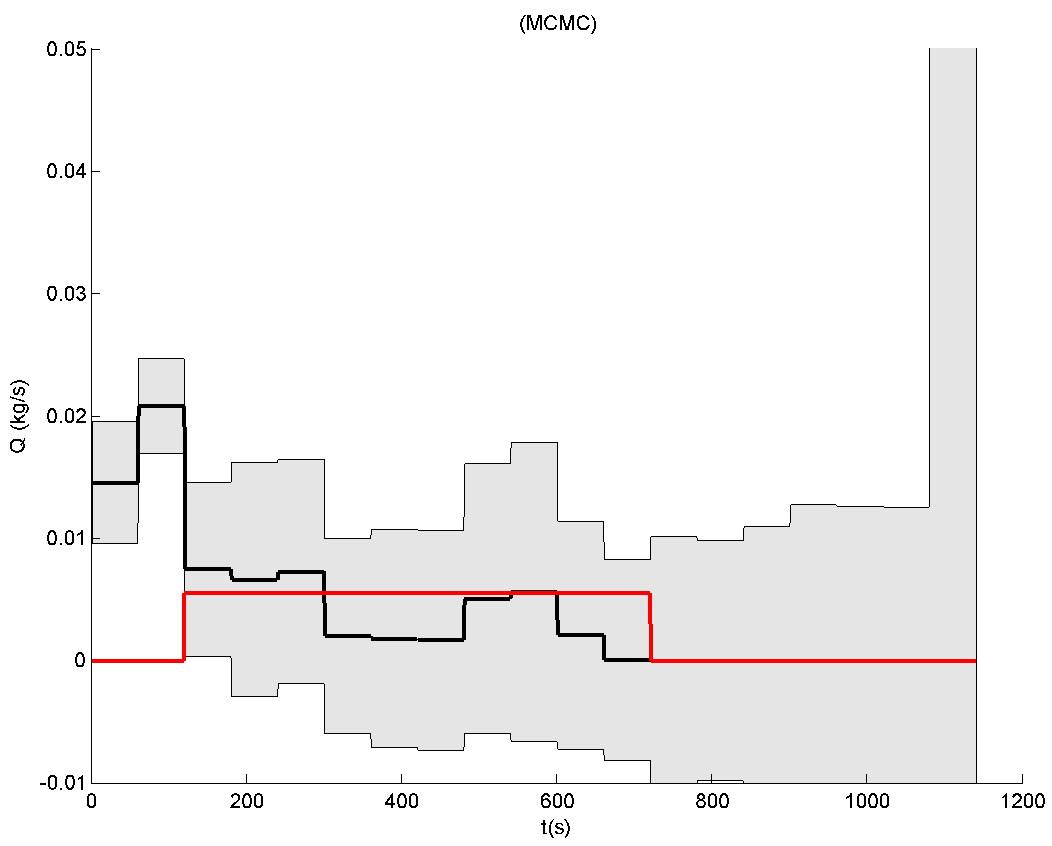
\includegraphics[width=1\textwidth]{fig_15_B}
		\caption{MCMC}
		\label{fig_15_B}
	\end{subfigure}
	\caption{Estimation du profil d'émission du \textit{trial} 7 (en noir), intervalle de confiance à $\pm 2\widetilde{\sigma}_q$ (en gris) et comparaison avec les valeurs réelles (en rouge), avec AMIS (\ref{fig_15_A}) et MCMC (\ref{fig_15_B}).}
	\label{fig_15_AE} 
\end{figure}

\section{Conclusions}

L'étude de cas sur l'expérience FFT07 présentée dans ce chapitre a permis une première validation de la méthodologie axée sur l'algorithme AMIS. Celle-ci a en effet permis une bonne estimation de la position de la source dans les cas synthétiques et expérimentaux,  en fournissant une distribution a posteriori des coordonnées de la source. Cet outil statistique permet ainsi d'effectuer une analyse autour des incertitudes associées à l'estimation, \NdPA{tout en permettant un accès à l'information ponctuelle} par le biais du calcul de l'estimateur MMSE. \\

 La démarche et a également permis de reconstruire un profil d'émission complet, fournissant une information temporelle sur les quantités émises par la source ainsi que ses temps de démarrage et d'arrêt. Cet aspect temporel présente un aspect innovant par rapport aux approches conventionnelles présentées dans la littérature, où l'hypothèse d'un débit d'émission constant est formulée, se traduisant dans la pratique par la recherche d'une unique valeur scalaire $q$. 
 
Cette étude a démontré que la quasi-totalité de la charge de calcul est concentrée sur la construction des matrices source-récepteur, plus précisément sur les appels au modèle de dispersion. Dans le cas d'un modèle gaussien les temps de calcul demeurent raisonnables, mais ils dépendent directement du nombre de particules échantillonnées par itération de l'AMIS. Nous avons pu vérifier que le fait de tirer plus de 100 particules par itération dans cette étude de cas n'améliorait pas significativement les résultats d'estimation \NdPA{en termes de précision}, mais dans le cadre général un nombre trop faible de particules pourrait dégrader la qualité de l'estimation, car l'exploration de l'espace des paramètres s'en trouverait restreinte. De plus, à nombre égal de particules, si le contexte exige l'utilisation d'un modèle de dispersion plus élaboré (par exemple dans un milieu urbain), la charge et le temps de calcul seront bien plus importants. \\

\NdFS{Il devient ainsi nécessaire d'optimiser à la fois le mode d'usage du modèle de dispersion ainsi que l'exploration des différentes valeurs possibles pour les particules. Ces deux points sont abordés dans le Chapitre 4, qui présente une nouvelle façon d'obtenir les résultats des calculs de dispersion, ainsi qu'une initialisation améliorée de la loi de proposition.}



	
	\chapter{Calcul des matrices source-récepteur par un modèle lagrangien adjoint}

L'étude de cas sur l'expérience FFT07 présentée dans le Chapitre 3 a montré que la charge de calcul de la procédure d'estimation du terme source est en grande majorité focalisée sur le calcul de la matrice source-récepteur. Cette étape nécessite une quantité d'appels au modèle de dispersion égale au nombre de particules échantillonnées par itération multiplié par le nombre d'itérations, soit en pratique 1000 instances dans le cas de FFT07. \\

Si pour les cas les plus simples il est possible de se limiter à des modèles de dispersion suffisamment rapides, la situation change dès qu'il s'agit de considérer un contexte plus élaboré, avec des outils de calculs permettant certes une meilleure représentation des phénomènes de dispersion, mais dont l'exécution devient bien plus coûteuse en termes d'implémentation et de temps de calcul. \\

L'objet de ce chapitre est ainsi de présenter une façon d'optimiser le calcul des matrices source-récepteur lorsque celui-ci doit faire appel à un code de dispersion plus complexe que le modèle à bouffées gaussiennes précédemment évoqué. La présentation de cet outil de calcul constituera la première partie de ce chapitre, avec notamment une explication de son fonctionnement, puis une présentation de son intégration optimale à la chaîne de calcul et d'estimation existante. La suite du chapitre se concentrera sur les aspects pratiques autour de la mise en application de cette méthodologie améliorée, avec la présentation des résultats sur plusieurs cas-tests de simulation.


\section{Le code de calcul PMSS}

\subsection{L'approche lagrangienne de la dispersion atmosphérique}
\label{part_lagrangian}

Pour les modèles dits eulériens, la résolution du problème de la dispersion d'un polluant dans l'atmosphère passe par la construction d'un maillage sur le domaine étudié, afin de pouvoir observer l'évolution des concentrations du polluant porté par les mouvements de l'air. 

Le point de vue lagrangien est différent: il s'agit ici de résoudre un système d'équations dans un repère lié au déplacement de la masse d'air contenant le polluant. Pour cela, on représente le panache sous la forme d'un ensemble de \textit{particules lagrangiennes}\footnote{Afin d'éviter toute confusion avec les particules statistiques dont il est fait référence dans le cadre de l'algorithme AMIS, nous utiliserons la dénomination  de \textit{particule lagrangienne} abréviée par PL dans la suite du texte. Nous conservons le terme de \textit{particule} pour désigner les échantillons issus de l'AMIS.}, chacune étant porteuse d'une masse élémentaire du polluant considéré. Le principe d'un modèle lagrangien consiste ainsi à étudier les trajectoires de ces éléments discrets dans le domaine au fil du temps.

Le fait de modéliser le panache par un ensemble de PL permet de tenir compte de la nature stochastique de leur déplacement, qui traduit la variabilité inhérente aux processus de turbulences auxquels est soumis le panache: on parle d'ailleurs plus précisément de \textit{modèle lagrangien stochastique}. On va ainsi travailler sur une équation de transport portant sur la densité de probabilité associée à chaque trajectoire. Plus formellement, d'après \cite{Flesch1995}, la formulation classique régissant un modèle de dispersion lagrangien se présente sous la forme d'une équation de Langevin, qui s'écrit: 

\begin{equation}
	\begin{split}
		du_i &= a_i(\Vecx, \Vecu, t)dt + b_{i,j}(\Vecx, \Vecu, t)d\xi_j  \\
		dx_i &= u_i dt = (\bar{u}_i + U_i)dt
	\end{split}
	\label{eq_langevin}
\end{equation}
où:
 \begin{itemize}
	\item $\Vecx = (x, y, z)$ est la position de la PL  définie par un repère spécifique: $x$ suit l'axe du vent, $y$ suit l'axe perpendiculaire au vent, et $z$ désigne l'élévation verticale classique. 
	\item $\Vecu$ est la vitesse d'écoulement à laquelle est soumise la PL: $\Vecu = (u, v, w)$ où les composantes respectives de ce vecteur suivent les mêmes axes que $\Vecx$.
	\item $a_i$ et $b_{i,j}$ sont des fonctions spécifiques de $(\Vecx, \Vecu, t)$ respectivement appelées \textit{drift term} et \textit{random forcing}.
	\item $d\xi_j$ est un incrément aléatoire suivant une distribution gaussienne de moyenne nulle et de variance $dt$.
	\item $\bar{u}_i$ représente le vent moyen et $U_i$ sa composante stochastique.
	
\end{itemize}

L'expression des fonctions $a_i$ et $b_{i,j}$ varie selon les hypothèses que l'on se fixe sur la nature de la turbulence: une présentation plus détaillée de leur calcul est disponible dans \cite{Wilson1996}. Une fois que ceux-ci sont définis,l'équation \eqref{eq_langevin} est discrétisée et sa résolution permet de calculer un ensemble de trajectoires de PL émanant d'une source dont les paramètres sont connus. Les concentrations volumiques moyennes simulées sont alors obtenues par la somme des particules présentes dans un volume élémentaire $d\Vecx$ autour du point d'observation $\Vecx$ durant un certain temps de résidence. En d'autres termes, on peut écrire la concentration moyenne au point $\Vecx$ et à l'instant $t$ comme étant : 

\begin{equation}
	C(\Vecx, t) = \int _{-\infty}^{t} \int_{V} S(\Vecx',t')p(\Vecx, t | \Vecx', t')d\Vecx'dt
	\label{eq_c_moyen_lagrangien}
\end{equation}
où $V$ est le volume défini par le domaine d'étude, $S(\Vecx',t')$ est la distribution de la source, et $p(\Vecx, t | \Vecx', t')$ est la densité de probabilité sur la position $\Vecx$ et l'instant $t$ des PL de position initiale $\Vecx'$ à l'instant $t'$. \\

\begin{figure}
	\centering
	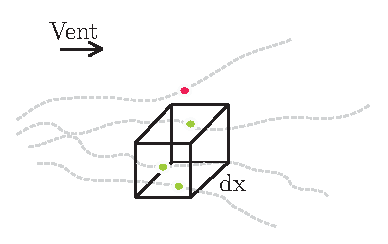
\includegraphics[width=0.65\textwidth]{lagrangian_ok}
	\caption{Principe du modèle lagrangien: la concentration en $\Vecx$ s'obtient par la somme des PL (en vert) traversant le volume élémentaire $d\Vecx$ durant un certain temps de résidence.}
	\label{fig_schema_lagrangien}
\end{figure}

Afin de calculer le champ d'écoulement auquel sont soumises les PL, plusieurs méthodes sont disponibles. Il est par exemple possible de résoudre les équations de la mécanique des fluides via un outil de simulation de type CFD, ce qui permet une modélisation fine des phénomènes physiques mis en jeu. Une autre possibilité consiste à avoir recours à une simulation dite \textit{CFD simplifiée}, où le champ de vent est interpolé à partir des mesures d'une ou plusieurs stations météorologiques tout en prenant en compte la topographie du terrain. C'est cette dernière approche qui est employée dans les outils de calcul du CEA et d'ARIA Technologies, et que nous présentons dans le chapitre suivant. \\

\subsection{La chaîne de calcul SWIFT-SPRAY}

L'outil \textit{Parallel Micro-SWIFT-SPRAY} (PMSS) est une chaîne de calcul constituée de deux éléments distincts: un outil de CFD simplifiée (SWIFT) et un modèle de dispersion lagrangien stochastique (SPRAY). Il est généralement appliqué dans des études à petite échelle (par exemple, au niveau d'un quartier), mais grâce à sa version parallèle, il a récemment été utilisé sur des domaines plus grands, à l'exemple du cas AirCity (REF) où le modèle a été exécuté sur l'ensemble de la ville de Paris.\\

\subsubsection{SWIFT}

Le modèle SWIFT permet de produire des champs de vent 3D en exploitant différents types de données météorologiques sur un même site (profils de vent et de température, stations de mesures, sorties de modèles météorologiques de prévision). Il permet notamment de prendre en compte la topographie du milieu, la présence d'obstacles tels que des bâtiments, l'occupation des sols ou encore l'influence de la stabilité atmosphérique. Son fonctionnement peut être résumé en quatre étapes :  \\

\begin{enumerate}
	\item Dans un premier temps, les mesures météorologiques reçues en entrée sont interpolées sur les différents points constituant une version discrétisée du domaine.
	\item Dans un deuxième temps, l'effet des obstacles présents dans le domaine sur l'écoulement sont modélisés via la création de zones spécifiques dans le voisinage de ces obstacles où le champ de vitesse est calculé de façon spécifique.
	\item La troisième étape consiste à ajuster le champ de vent en appliquant un principe de conservation de la masse.
	\item Enfin, la dernière étape consiste à calculer la turbulence intrinsèque à l'écoulement modélisé.\\
\end{enumerate}

\begin{figure}[h!]
	\centering
	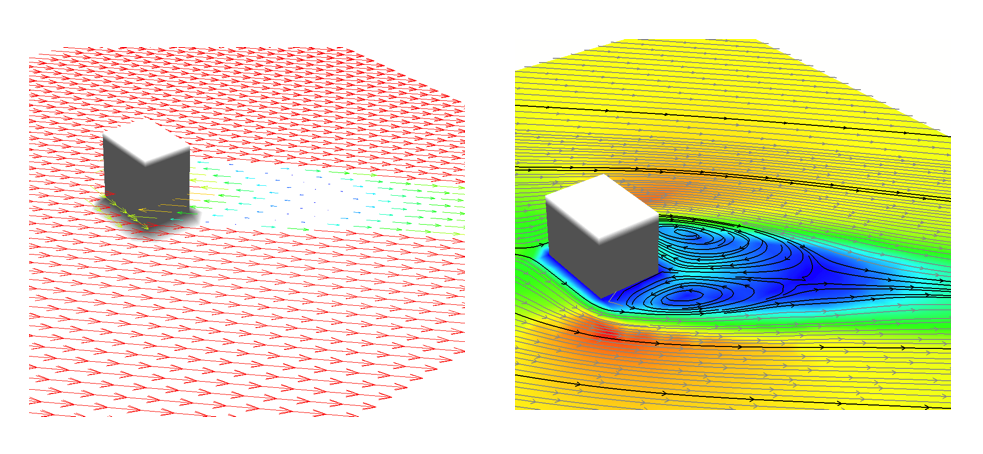
\includegraphics[width=0.75\textwidth]{swift_exemple}
	\caption{Exemple de calcul d'un champ de vent autour d'un obstacle avec SWIFT, avant (à gauche) et après (à droite) l'ajustement du champ}
	\label{fig_swift_exemple}
\end{figure}
En sortie de cet enchaînement de calculs, on obtient un champ de vent 3D qui peut alors directement être exploité par le modèle de dispersion SPRAY.



\subsubsection{SPRAY}

SPRAY est un modèle de dispersion lagrangien stochastique dont les principes de base suivent les mécanismes présentés à la section \ref{part_lagrangian}. L'implémentation de SPRAY repose sur le critère dit de \textit{well-mixed condition} permettant de donner une formulation explicite aux termes $a_i$ et $b_{i,j}$ de l'équation \eqref{eq_langevin} , et présenté en détail dans les travaux de \cite{Thomson1987}.

En pratique, plusieurs fonctionnalités supplémentaires sont implémentées dans SPRAY, telles que: \\

\begin{itemize}
	\item le "rebond" des particules sur les obstacles,
	\item le calcul de doses pour les sources radioactives,
	\item la prise en compte des différents types de dépôts (secs ou humides).\\
\end{itemize}

\begin{figure}[h!]
	\centering
	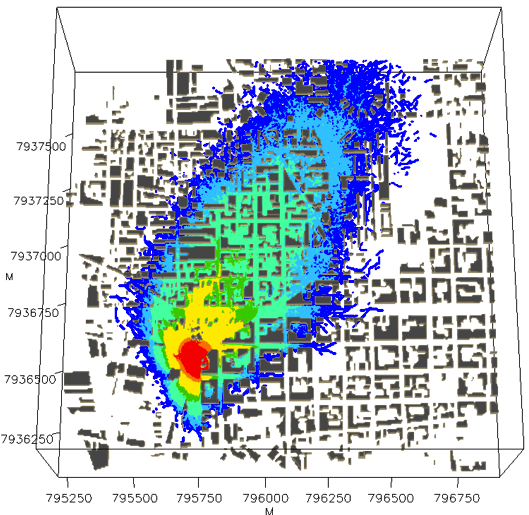
\includegraphics[width=0.65\textwidth]{spray_exemple}
	\caption{Exemple de champ de concentration calculé par SPRAY dans un domaine de type urbain}
	\label{fig_spray_exemple}
\end{figure}

La combinaison de SWIFT et SPRAY permet ainsi de calculer un champ de concentration sur le domaine étudié, connaissant les paramètres du terme source qui sont soumis en entrée du modèle SPRAY. Dans le contexte de ce chapitre, la chaîne de calcul PMSS permet de:

\begin{itemize}
	\item générer un jeu d'observations synthétiques en simulant un rejet induit par une source que l'on va chercher à retrouver: pour cela, on calcule les valeurs du champ de concentrations en un nombre fini de points du domaine que nous définirons comme étant les observations fournies par les capteurs,
	\item construire les matrices source-récepteur lors de l'exécution de l'algorithme AMIS, nécessaires au processus d'estimation du terme source.\\
\end{itemize}

\subsection{Dualité \textit{forward-backward}}

L'optimisation du calcul des matrices source-récepteur suivant le modèle de l'équation \eqref{eq_AE_4} est un point important: en effet dans une approche directe telle que présentée dans le chapitre précédent, la construction des $\MatC(\VecTheta)$ pour chaque particule $\VecTheta$ échantillonnée depuis la loi de proposition courante fait appel à autant de calculs de dispersion, ce qui rend l'opération d'estimation du terme source très coûteuse en temps de calcul.\\

Nous proposons dans la suite de ce chapitre une amélioration du processus d'estimation privilégiant le calcul des matrices source-récepteur par une approche de type \textit{backward}. Cette méthodologie a initialement été introduite dans \cite{Keats2007} pour ensuite être appliquée sur un algorithme d'estimation de type MCMC, nous en rappelons les bases ci-après.\\

Soit une source ponctuelle $Q$ située au point de l'espace $\PosSource$, de débit massique constant $q_s$ et de temps d'activation et d'arrêt respectifs $t_{on}$ et $t_{off}$ définie par la distribution suivante:\\

\begin{equation}
	Q = q_s \delta(\Vecx - \PosSource)\left[H(t - t_{on}) - H(t - t_{off})\right]
\end{equation}
où $\delta$ est la distribution de Dirac et $H$ la fonction de Heaviside. On note $C$ le champ de concentration moyen induit par cette  source. La valeur simulée de concentration $c_i$ obtenue sur le $i$-ème capteur à l'instant $t$ peut se modéliser par l'équation suivante:

\begin{equation}
c_i = \int_0^t \int_V C h ~dtdV
\label{eq_int_direct}
\end{equation}
où $h$ est la \textit{fonction} de réponse du capteur. Cette équation peut se simplifier sous la notation suivante:\\

\begin{equation}
c_i = \langle	C,h\rangle
\label{eq_scal_direct}
\end{equation} 

La relation de \textit{dualité forward-backward} présentée par \cite{Keats2007} stipule que cette même concentration peut s'écrire sous la forme:

\begin{equation}
c_i = \int_0^t \int_V Q C^* ~ dtdV = \langle Q, C^*\rangle
\label{eq_int_adjoint}
\end{equation}
où $C^*$ est le champ de rétro-concentrations induit par le $i$-ème capteur, et dont les valeurs sont obtenues par la résolution de l'équation \eqref{eqn_advection_diffusion_backward}. Dans la pratique, le champ $C^*$ est simulé par un \textit{modèle de dispersion dual}, ou \textit{modèle de rétro-dispersion}.\\

La relation de dualité $\langle C,h\rangle = \langle Q,C^* \rangle$ est ainsi valable si l'équation adjointe d'advection-diffusion a été résolue de telle sorte que les conditions aux limites permettent d'annuler les termes de bord pouvant y apparaître. De plus:

\begin{enumerate}
	\item sous l'hypothèse d'un capteur idéal, sa résolution est infinie, ce qui se traduit en pratique par $h$ prenant la forme d'une distribution de Dirac,
	\item dans le cadre de la construction des matrices source-récepteur, $Q$ illustre une source instantanée et dont le débit de rejet est unitaire.
\end{enumerate}

Dans ce cas particulier, on obtient alors une équivalence entre $C$ et $C^*$: 

\begin{equation}
C \simeq C^*
\label{eq_equivalence}
\end{equation}


\subsection{Intégration d'un modèle \textit{backward} au processus d'estimation}

\subsubsection{Utilisation de RetroSPRAY dans l'AMIS}

L'outil PMSS dispose d'une version \textit{backward} de SPRAY appelée RetroSPRAY, dont l'intégration dans la chaîne de calcul se fait de la même façon que pour SPRAY. Le modèle RetroSPRAY procède à la résolution des équations de Langevin en mode inverse: 

\begin{equation}
\begin{split}
du_i^b &= U_i^b (t-dt) - U_i^b(t) \\
dx_i^b &= x_i^b (t-dt) - x_i^b(t)
\end{split}
\label{eq_langevin_inv1}
\end{equation}

On peut alors écrire l'équivalent inverse de l'équation \eqref{eq_langevin} sous la forme suivante:

\begin{equation}
	\begin{split}
	du_i^b &= a_i^b dt + b_{i,j}^b d\xi_j \\
	dx_i^b &= -(\bar{u}_i + U_i^b )dt
	\end{split}
	\label{eq_langevin_inv2}
\end{equation}

Les termes $a_i^b$ et $ b_{i,j}^b$ peuvent être calculés selon les expressions fournies dans \cite{Flesch1995} et \cite{Wilson2009}. \\

Si on examine plus en détail la construction de la matrice source-récepteur, on peut réécrire l'équation \eqref{eq_AE_4} sous une forme plus explicite: notons $C(R_i,t_j |\VecTheta, t'_n)$ la concentration moyenne au capteur $R_i$ à l'instant $t_j$ résultant d'une source située à la position $\VecTheta$ et ayant émis un rejet unitaire à l'instant $t'_n$. La version \textit{forward} de la matrice source-récepteur pour $\VecTheta$ s'écrit:

\begin{equation}
\MatC^f(\VecTheta) = 
\begin{pmatrix}
C(R_1,t_1 | \VecTheta, t'_1) & C(R_1,t_1 | \VecTheta, t'_2) & \cdots & C(R_1, t_1 |\VecTheta, t'_{T_s}) \\
C(R_1,t_2 | \VecTheta, t'_1) & C(R_1,t_2 | \VecTheta, t'_2) & \cdots & C(R_1, t_2 |\VecTheta, t'_{T_s}) \\
\vdots & \vdots & & \vdots \\
C(R_1,t_{T_c} | \VecTheta, t'_1) & C(R_1,t_{T_c} | \VecTheta, t'_2) & \cdots & C(R_1, t_{T_c} |\VecTheta, t'_{T_s}) \\
C(R_2,t_1| \VecTheta, t'_1) & C(R_2,t_1 | \VecTheta, t'_2) & \cdots & C(R_2, t_1 |\VecTheta, t'_{T_s}) \\
\vdots & \vdots & & \vdots \\
\vdots & \vdots & & \vdots \\
C(R_{N_c},t_{T_c} | \VecTheta, t'_1) & C(R_{N_c},t_{T_c} | \VecTheta, t'_2) & \cdots & C(R_{N_c}, t_{T_c} |\VecTheta, t'_{T_s}) \\
\end{pmatrix}
\label{eq_matrix_forward}
\end{equation}

En appliquant la relation de dualité \textit{forward-backward}, dans l'espace dual où le modèle \textit{backward} opère, les sources deviennent des "rétro-capteurs", et les capteurs deviennent des "rétro-sources". On définit alors $C^*(\VecTheta,t'_n | R_i, t_j)$ comme la rétro-concentration mesurée au point $\VecTheta$ à l'instant $t'_n$ provenant d'une rétro-source située à la position $R_i$ et ayant émis un rétro-rejet unitaire à l'instant $t_j$. La version \textit{backward} de $\MatC^f$ s'écrit alors:

\begin{equation}
\MatC^b (\VecTheta)= 
\begin{pmatrix}
	C^*(\VecTheta, t'_1 | R_1, t_1) & C^*(\VecTheta, t'_2 | R_1, t_1) & \cdots & C^*(\VecTheta, t'_{T_s} | R_1, t_1) \\
	C^*(\VecTheta, t'_1 | R_1, t_2) & C^*(\VecTheta, t'_2 | R_1, t_2) & \cdots & C^*(\VecTheta, t'_{T_s} | R_1, t_1) \\
	\vdots & \vdots & & \vdots \\
	C^*(\VecTheta, t'_1| R_1,t_{T_c}) & C^*(\VecTheta, t'_2 | R_1, t_{T_c}) & \cdots & C^*(\VecTheta, t'_{T_s} | R_1, t_{T_c}) \\ 
	\vdots & \vdots & & \vdots \\
	\vdots & \vdots & & \vdots \\
	C^*(\VecTheta, t'_1| R_{N_c},t_{T_c}) & C^*(\VecTheta, t'_2 | R_{N_c}, t_{T_c}) & \cdots & C^*(\VecTheta, t'_{T_s} | R_{N_c}, t_{T_c}) \\ 
	
\end{pmatrix}
\label{eq_matrix_backward}
\end{equation}

Dans l'algorithme AMIS, au moment de calculer la vraisemblance de chaque particule échantillonnée, on peut ainsi faire désormais intervenir $\MatC^b$ comme matrice source-récepteur.

\subsubsection{Avantages}

Le fait de substituer un modèle \textit{backward} au modèle direct permet de n'avoir à faire qu'un seul calcul de rétro-dispersion par capteur, qui donne alors l'ensemble des valeurs de rétro-concentrations sur le domaine. De plus, ces calculs sont désormais opérés en amont du schéma itératif de l'AMIS: au lieu d'exécuter une boucle qui lance des calculs de dispersion pour chaque particule AMIS et à chaque itération, les champs $C^*$ sont pré-calculés et déjà disponibles au moment de l'estimation du terme source. \\

\begin{figure}[h!]
	\centering
	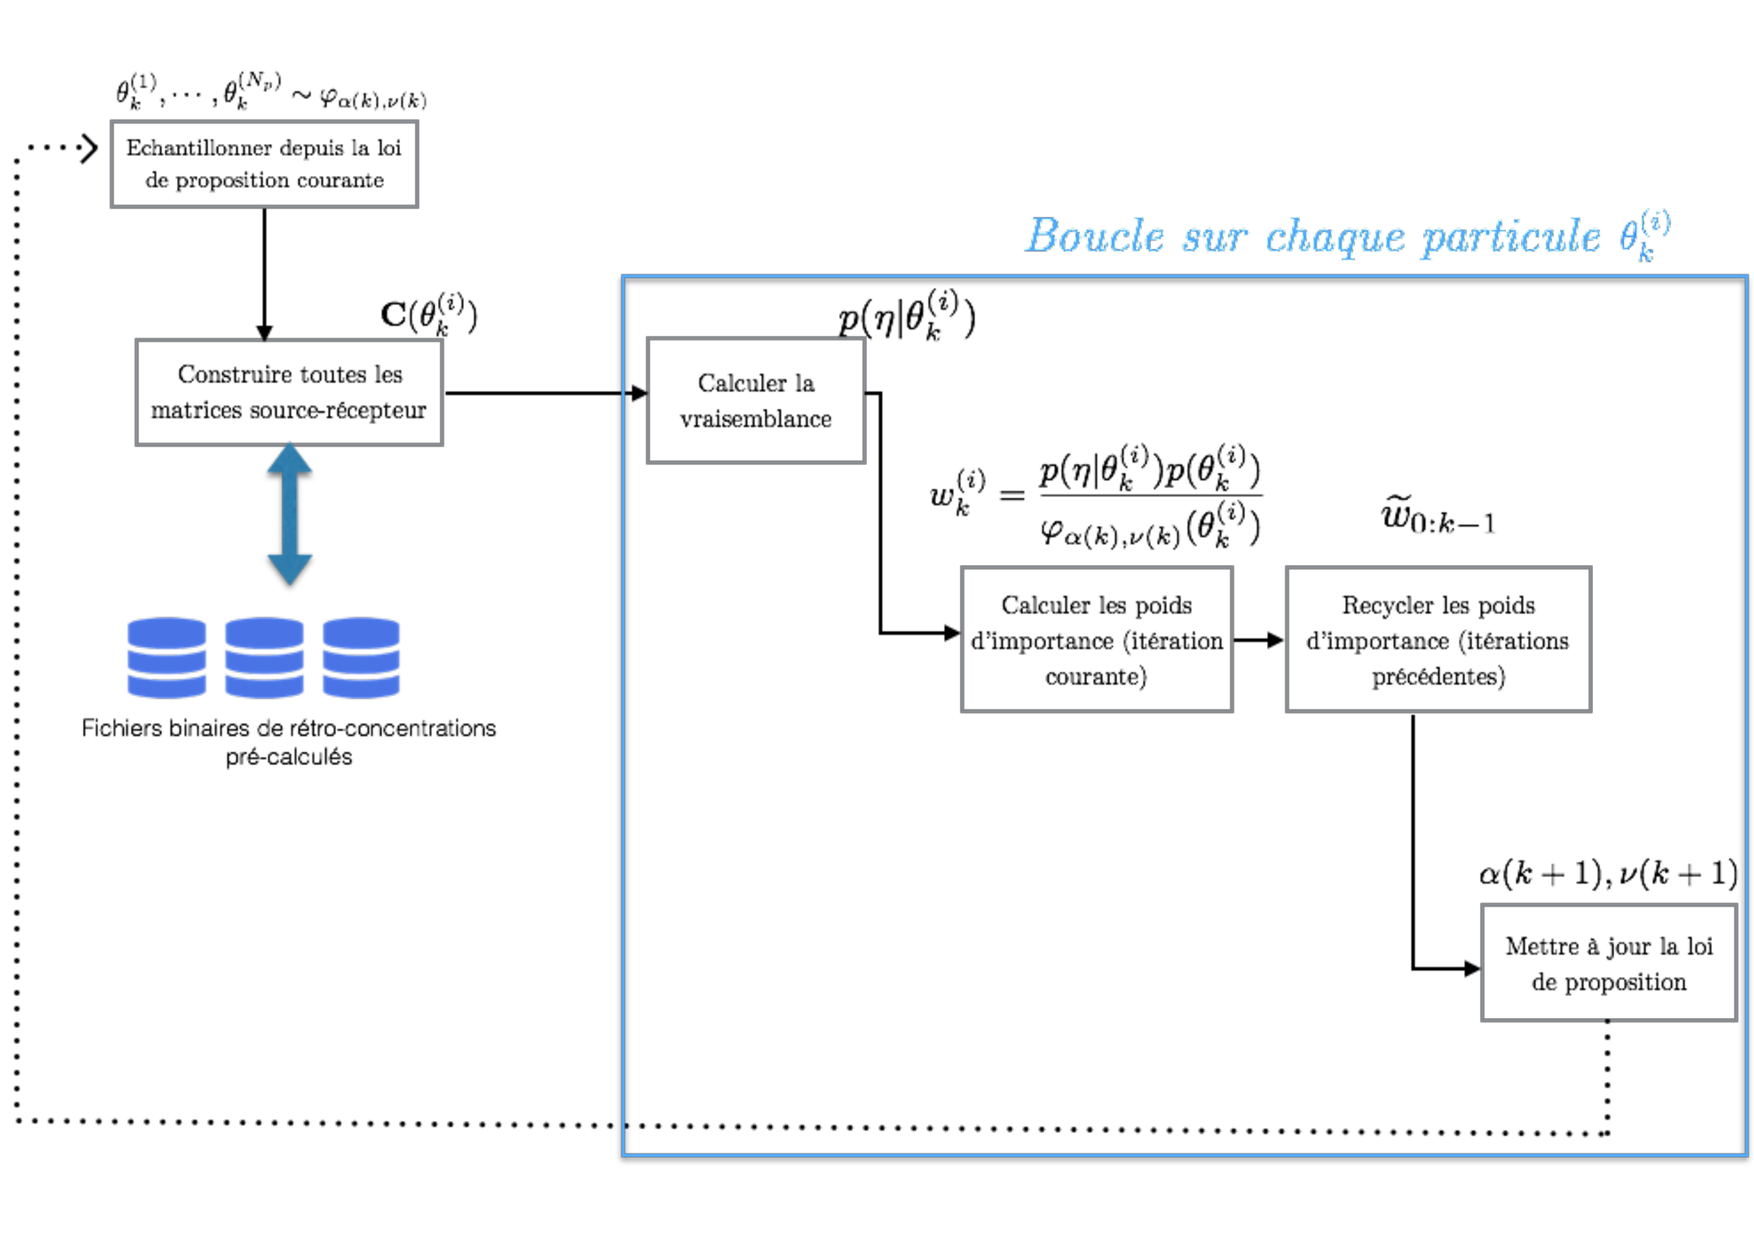
\includegraphics[width=0.75\textwidth]{schema_amis_optimise}
	\caption{Schéma de principe de la version \textit{backward} de l'algorithme d'estimation du terme source}
	\label{fig_schema_amis_optimise}
\end{figure}

Comme l'illustre la figure \ref{fig_schema_amis_optimise}, aucun calcul de dispersion n'est donc instancié durant la mise en oeuvre de l'algorithme, car les matrices source-récepteur sont désormais construites grâce à des opérations de lecture des fichiers dans lesquels ont été stockés les valeurs de $C^*$ pré-calculées. PMSS permet en effet d'agréger les résultats des calculs de dispersion dans des fichiers binaires, qui servent de base de données où les valeurs de rétro-concentration en chaque point du domaine peuvent être lues par un module d'entrée/sortie intégré à l'implémentation de l'AMIS.

Même si cette opération n'est plus directement intégrée à l'algorithme d'estimation, elle demande néanmoins une certaine quantité de calculs. Cette dernière peut toutefois être réduite si on choisit de paralléliser l'opération de génération des fichiers binaires de rétro-concentration. Comme il s'agit de tâches parfaitement indépendantes les unes par rapport aux autres, la parallélisation est facilement réalisable (\textit{embarrasingly parallel jobs}). Si on doit générer $n_b$ fichiers binaires en allouant $n_p$ coeurs de calcul par opération de génération, cela requiert la disponibilité de $n_b \times n_p$ coeurs. Si une telle quantité de ressources n'est pas immédiatement disponible, il peut être plus judicieux de créer séquentiellement ces fichiers binaires. L'approche séquentielle est également à privilégier si on ne dispose pas d'une architecture de type \textit{cluster} permettant une parallélisation massive. \\


Il est néanmoins important de rappeler que le fait d'associer le modèle \textit{backward} au modèle direct constitue une approximation. En effet, la partie "diffusion" du processus de dispersion atmosphérique est aléatoire, et ne peut être parfaitement reproduite dans le cas dual pour une configuration identique du modèle direct, créant ainsi un écart incompressible entre les champs $C$ et $C^*$. 

Cet écart peut être minimisé en utilisant un nombre de PL suffisamment grand pour modéliser les rétro-rejets. Il faut toutefois prendre garde à ne pas choisir une grandeur trop élevée, qui demanderait un temps de calcul trop important au modèle. 


\section{Exemple d'application en rase campagne}

Dans cette section nous présentons un première application sur une situation  simple dans un contexte non-urbain. Il s'agit d'un exemple synthétique dont les données et les paramètres sont issus d'une simulation ayant permis la validation du modèle RetroSPRAY.

\subsection{Présentation du cas-test}

Nous considérons ici un cas-test en milieu rural reproduisant une émission accidentelle depuis un site industriel dans une zone située près de la commune de Beaune, en Bourgogne, en présence d'une topographie réelle. 

\begin{figure}[h!]
	\centering
	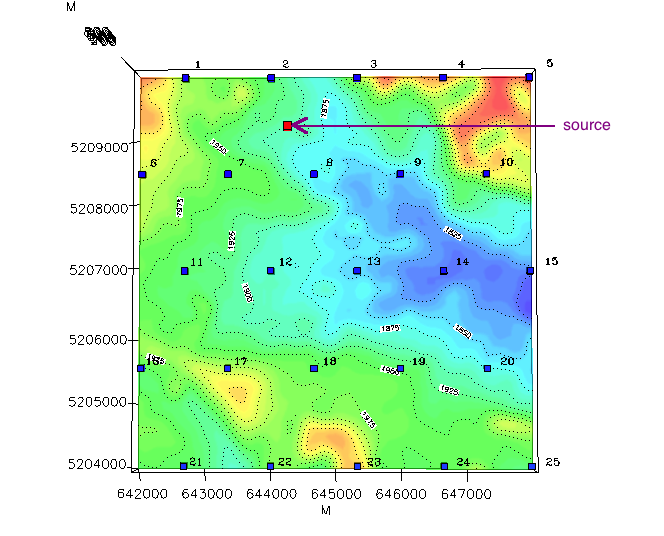
\includegraphics[width=0.8\textwidth]{beaune_relief_capteurs}
	\caption{Superposition du relief, de l'emplacement des capteurs et de la source du cas-test Beaune}
	\label{fig_beaune_relief}
\end{figure}

\subsubsection{Caractéristiques du domaine}
Le domaine considéré couvre une surface de \SI{6}{\square\kilo\meter} avec une source unique et un réseau relativement dense de 25 capteurs disposés en quinconce et couvrant toute la superficie du domaine (figure \ref{fig_beaune_relief}).

Pour la simulation, le domaine est discrétisé en une grille de $300 \times 300$ mailles, avec une résolution du maillage en $x$ et $y$ de \SI{20}{\meter}.

\subsubsection{Paramètres météorologiques}
Sur toute la durée de la simulation, nous considérons un vent constant en vitesse (\SI{1.5}{\m\per\second}) et en direction ($330\degres$). Le champ de vent produit par SWIFT est ainsi relativement homogène, comme observé en figure \ref{fig_beaune_vent}.

\begin{figure}[h!]
	\centering
	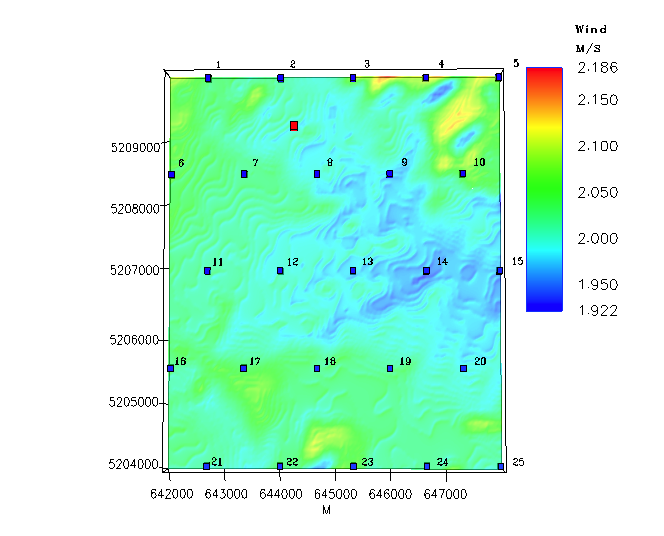
\includegraphics[width=0.8\textwidth]{beaune_vent}
	\caption{Champ de vent calculé par SWIFT pour le cas-test Beaune}
	\label{fig_beaune_vent}
\end{figure}


\subsubsection{Capteurs, source et simulation des observations}
On considère un réseau de 25 capteurs disposés de façon à couvrir tout le domaine, et placés à une hauteur de \SI{10}{\meter}, égale à celle de la source. Chaque capteur fournit des observations de concentrations moyennes entre 10h05 et 12h00, avec une plage de moyennage de 5 minutes.

Concernant la source, celle-ci est placée dans la partie nord (voir figure \ref{fig_beaune_relief}) afin que le panache résultant couvre une partie suffisante du domaine. Elle est située à une altitude de \SI{10}{\m}, identique à celle des capteurs: lors du processus d'estimation, on fait l'hypothèse que cette information est connue afin de limiter la reconstruction de la position aux coordonnées $(x,y)$. La source émet un rejet unique entre 10h15 et 11h, avec un débit constant de 1850 unités/s. \\

Il existe trois façons possibles de simuler le vecteur d'observation $\VecObs$ avec PMSS: 

\begin{enumerate}
	\item en spécifiant directement à SPRAY la position voulue pour la source ainsi que ses paramètres temporels d'émission,
	\item en calculant une matrice source-récepteur \textit{forward} $\MatC^f$ via SPRAY à la position voulue, puis en multipliant cette matrice par le profil d'émission $\VecQSource$ désiré,
	\item en calculant une matrice source \textit{backward} $\MatC^b$ via RetroSPRAY à la position voulue, puis en multipliant cette matrice par le profil d'émission $\VecQSource$ désiré.\\
	
\end{enumerate}

Si les représentations 1. et 2. sont équivalentes, la correspondance entre 2. et 3. n'est cependant pas immédiate : 

\begin{itemize}
	\item dans les configurations \textit{forward}, on définit un volume élémentaire $\Delta v_s^f$ pour la source et un volume de contrôle $\Delta v_c^f$ pour chacun des capteurs,
	\item dans le cas \textit{backward}, il faut également attribuer un volume élémentaire $\Delta v_s^b$ pour les rétro-sources et un volume de contrôle $\Delta v_c^b $ pour les points où sont simulés les concentrations conjuguées.\\
	
\end{itemize}

Pour avoir équivalence entre 2. et 3., il faut alors avoir: 

\begin{equation}
\begin{split}
\Delta v_s^f &= \Delta v_c^b \\
\Delta v_c^f &= \Delta v_s^b
\end{split}
\label{eq_dim_volumes}
\end{equation}

Or les paramètres d'origine de la simulation du cas-test Beaune spécifiaient des valeurs différentes pour $\Delta v_s^f$ (\SI{15}{\meter}$\times$\SI{15}{\meter}$\times$\SI{10}{\meter}) et $\Delta v_c^b$ (\SI{20}{\meter}$\times$\SI{20}{\meter}$\times$\SI{10}{\meter}) . Les résultats de la figure \ref{fig_comparaison_3_obs} reflètent ainsi les divergences engendrées par le non-respect des conditions \eqref{eq_dim_volumes}.

\begin{figure}[h!]
	\centering
	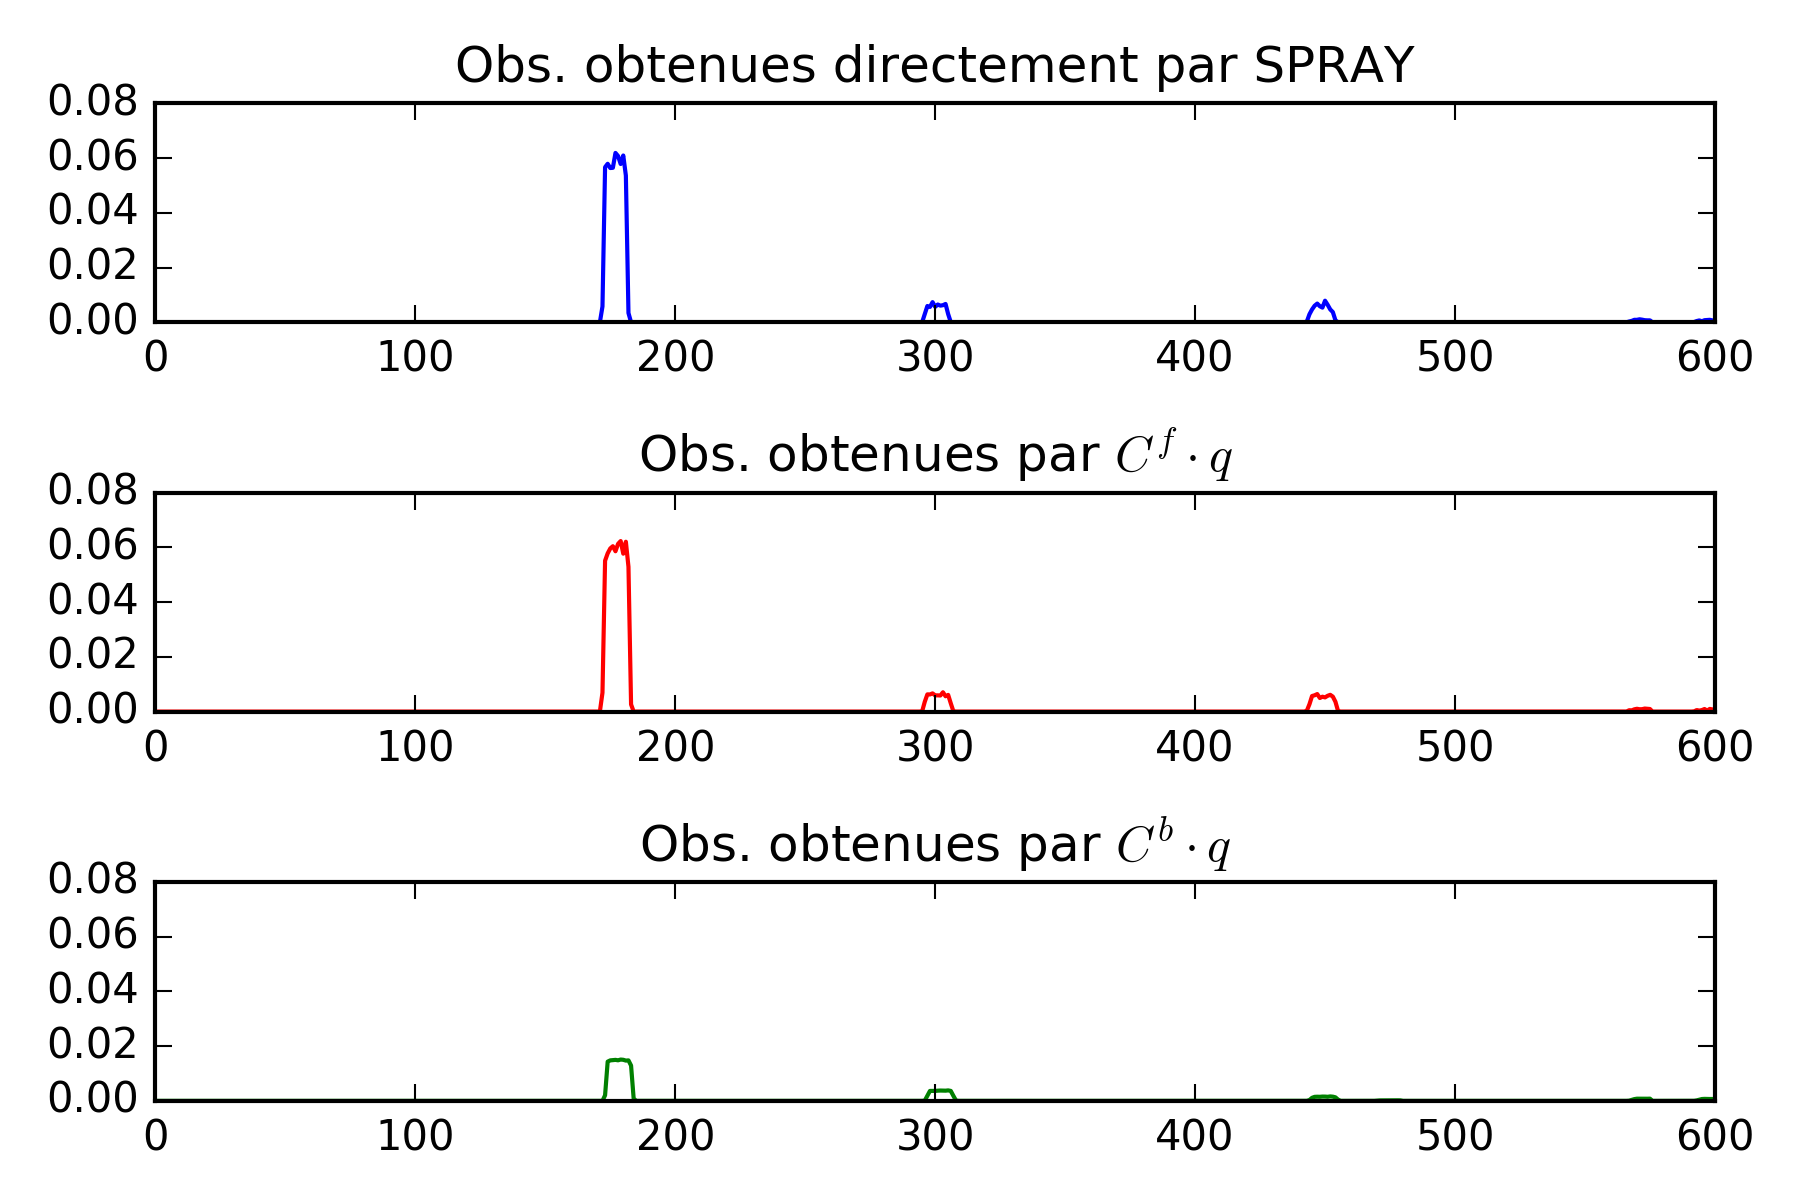
\includegraphics[width=0.8\textwidth]{comparaison_3_obs.png}
	\caption{Cas-test Beaune: différents modes de construction du vecteur $\VecObs$}
	\label{fig_comparaison_3_obs}
\end{figure}

Pour remédier à cela, on choisit alors de représenter la source comme un volume de dimension $\Delta v_c^b$ (autrement dit la source choisie couvre toute une maille du domaine), et d'utiliser la matrice source-récepteur \textit{backward} pour générer les observations. Cela permet en outre de s'assurer que la construction de $\VecObs$ est compatible avec la représentation des rétro-concentrations qui est utilisée dans l'algorithme d'estimation pour calculer la vraisemblance $p(\VecObs | \VecTheta)$ de chaque particule $\VecTheta$ tirée depuis la loi de proposition. Les mesures simulées par capteur sont représentées en figure \ref{fig_observations_25CAPTEURS}.

\begin{figure}[h!]
	\centering
	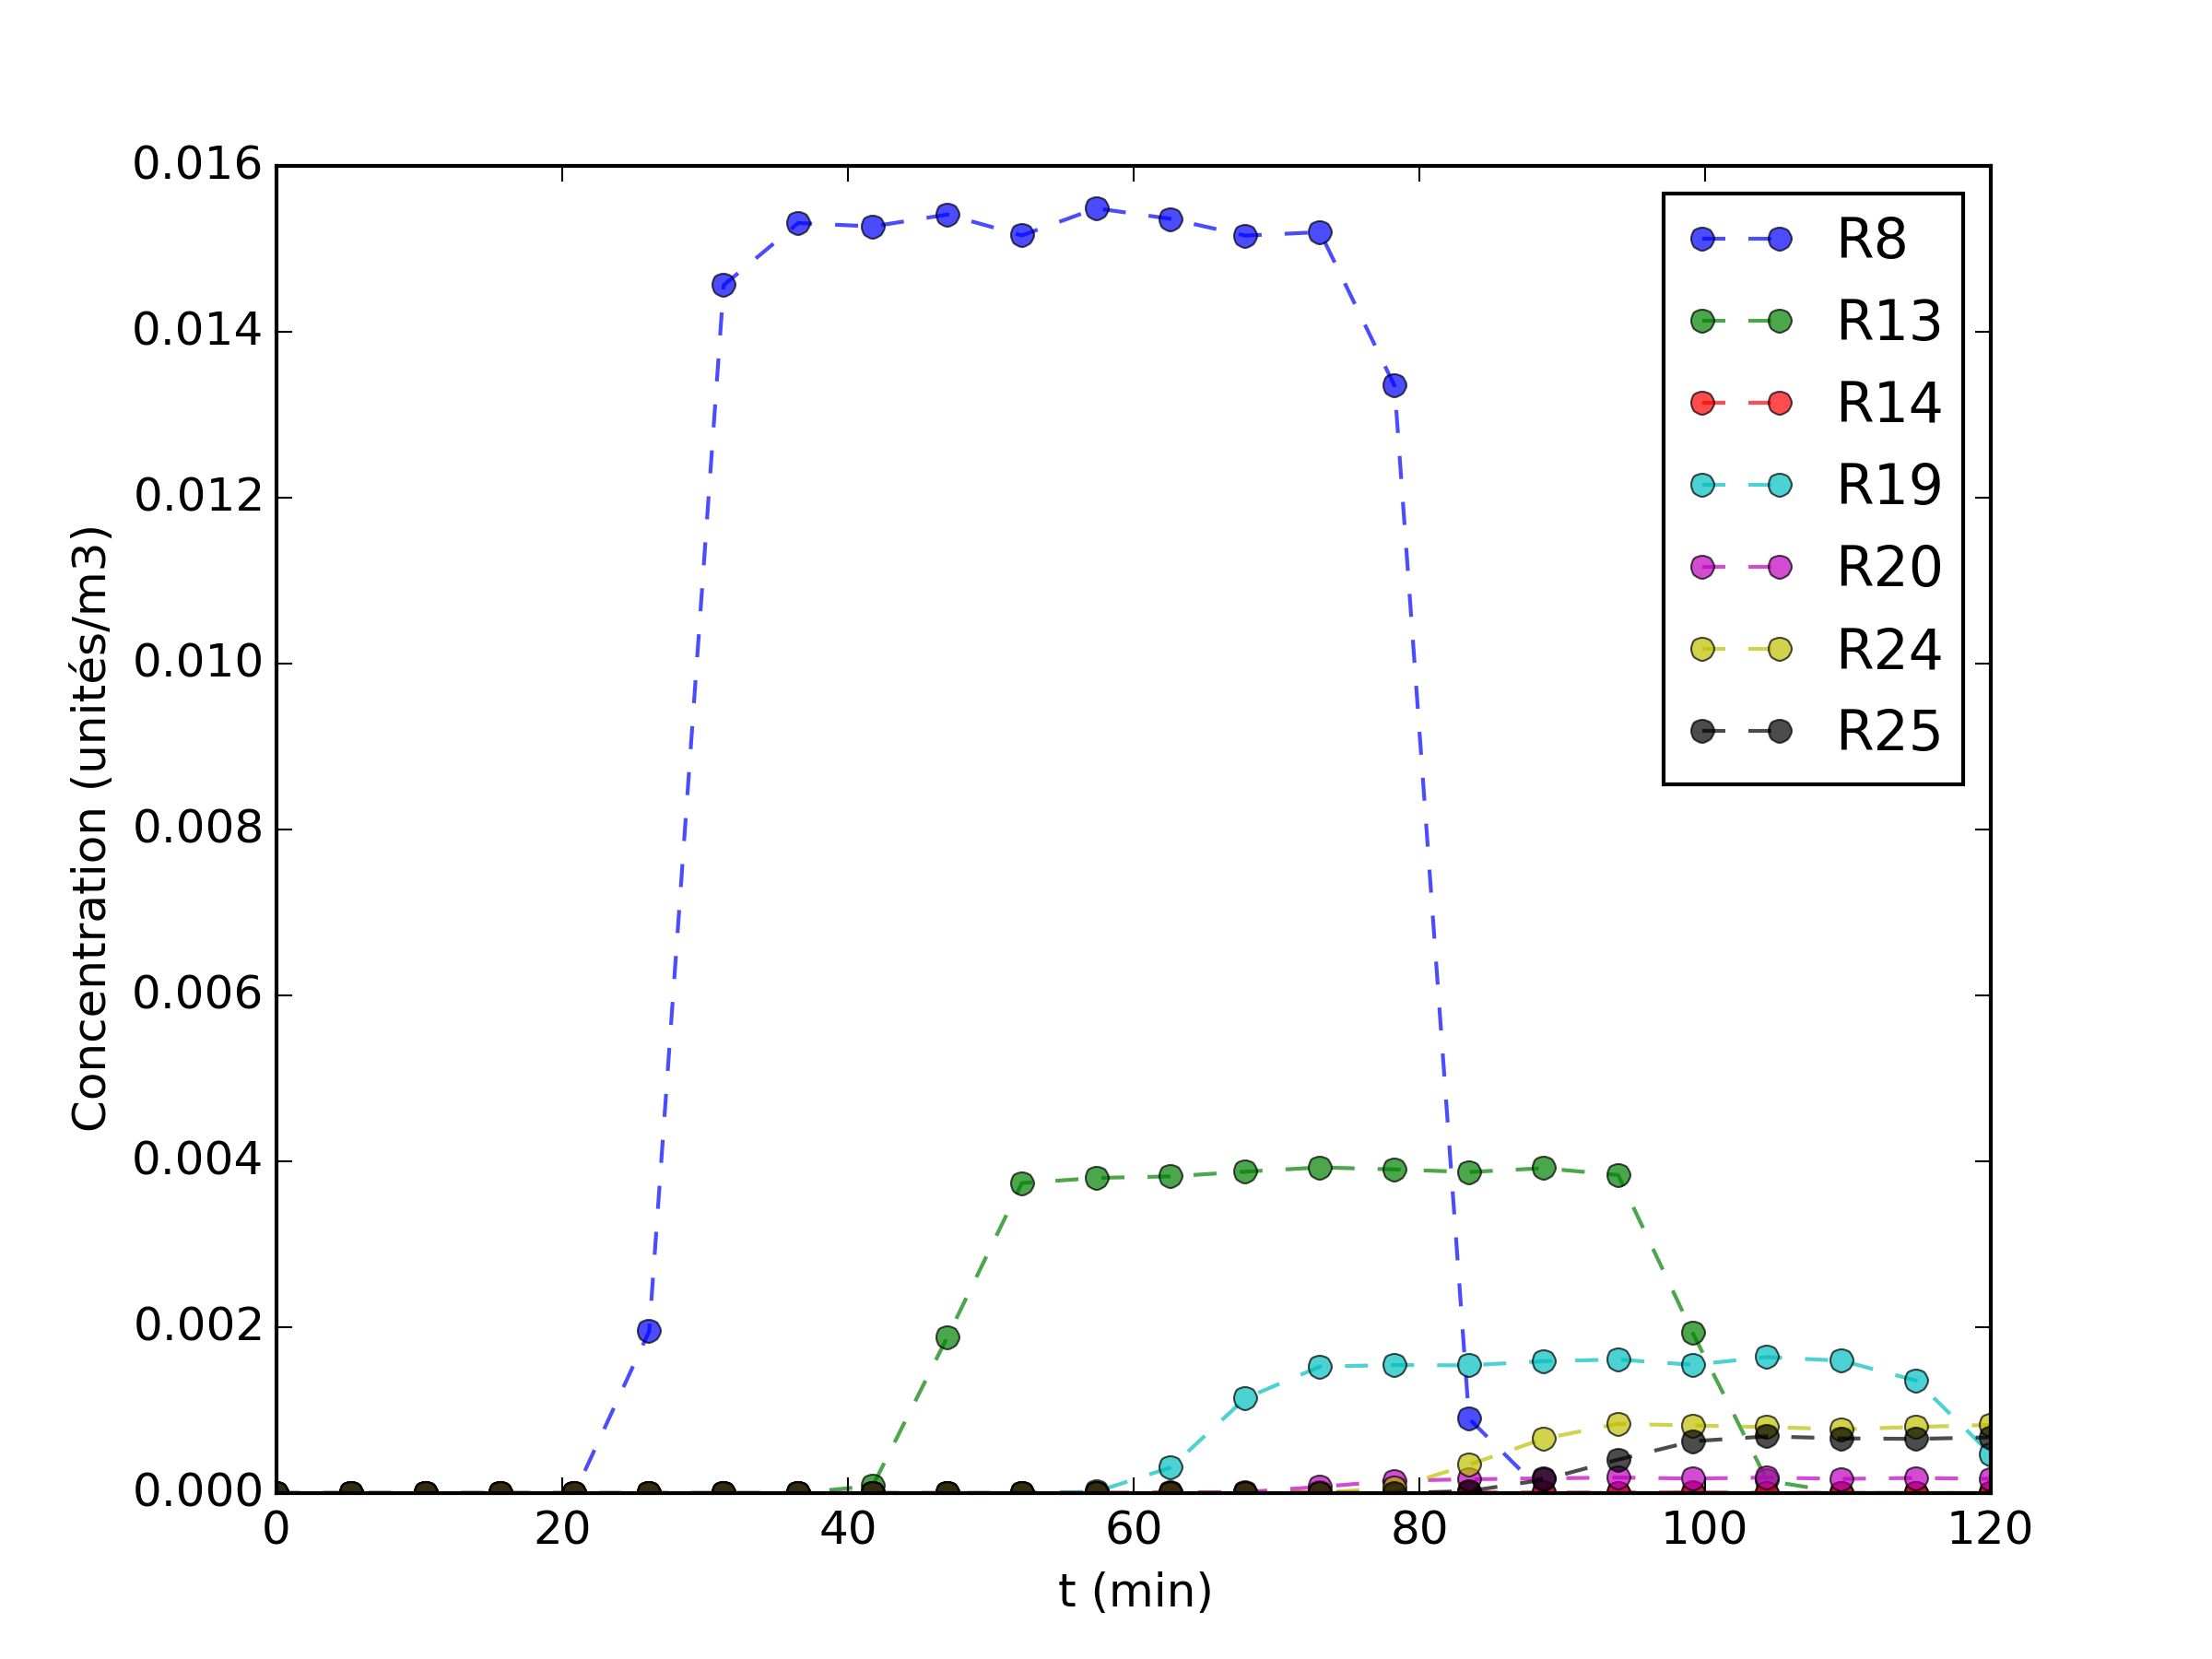
\includegraphics[width=0.8\textwidth]{concentrations_beaune.png}
	\caption{Cas-test Beaune: concentrations mesurées aux capteurs}
	\label{fig_observations_25CAPTEURS}
\end{figure}

\subsubsection{Premiers résultats}

Un \textit{run} préliminaire de l'AMIS servant de \textit{benchmark} a été lancé avec les paramètres suivants:
\begin{itemize}
	\item 10 itérations,
	\item 100 particules générées par itération,
	\item $\varObs = 2\times 10^{-6}$, qui fixe un degré d'incertitude suffisant autour des observations de la figure \ref{fig_observations_25CAPTEURS},
	\item une discrétisation temporelle de la source par paliers de 5 minutes, avec les paramètres a priori $\VecMeanQ = (0,\cdots,0)$ et $\varQ = 2\times 10^6$.
\end{itemize}

Avec ces paramètres, l'algorithme d'estimation parvient à fournir une reconstruction relativement correcte des paramètres, aussi bien concernant la localisation de la source (figures \ref{fig_25C_prelim_X} et \ref{fig_25C_prelim_Y}) que la reconstruction de son profil d'émission (figure \ref{fig_25C_prelim_Q}).\\

 \begin{figure}[h!]
 	\centering
 	\begin{subfigure}[t]{0.5\textwidth}
 		\centering
 		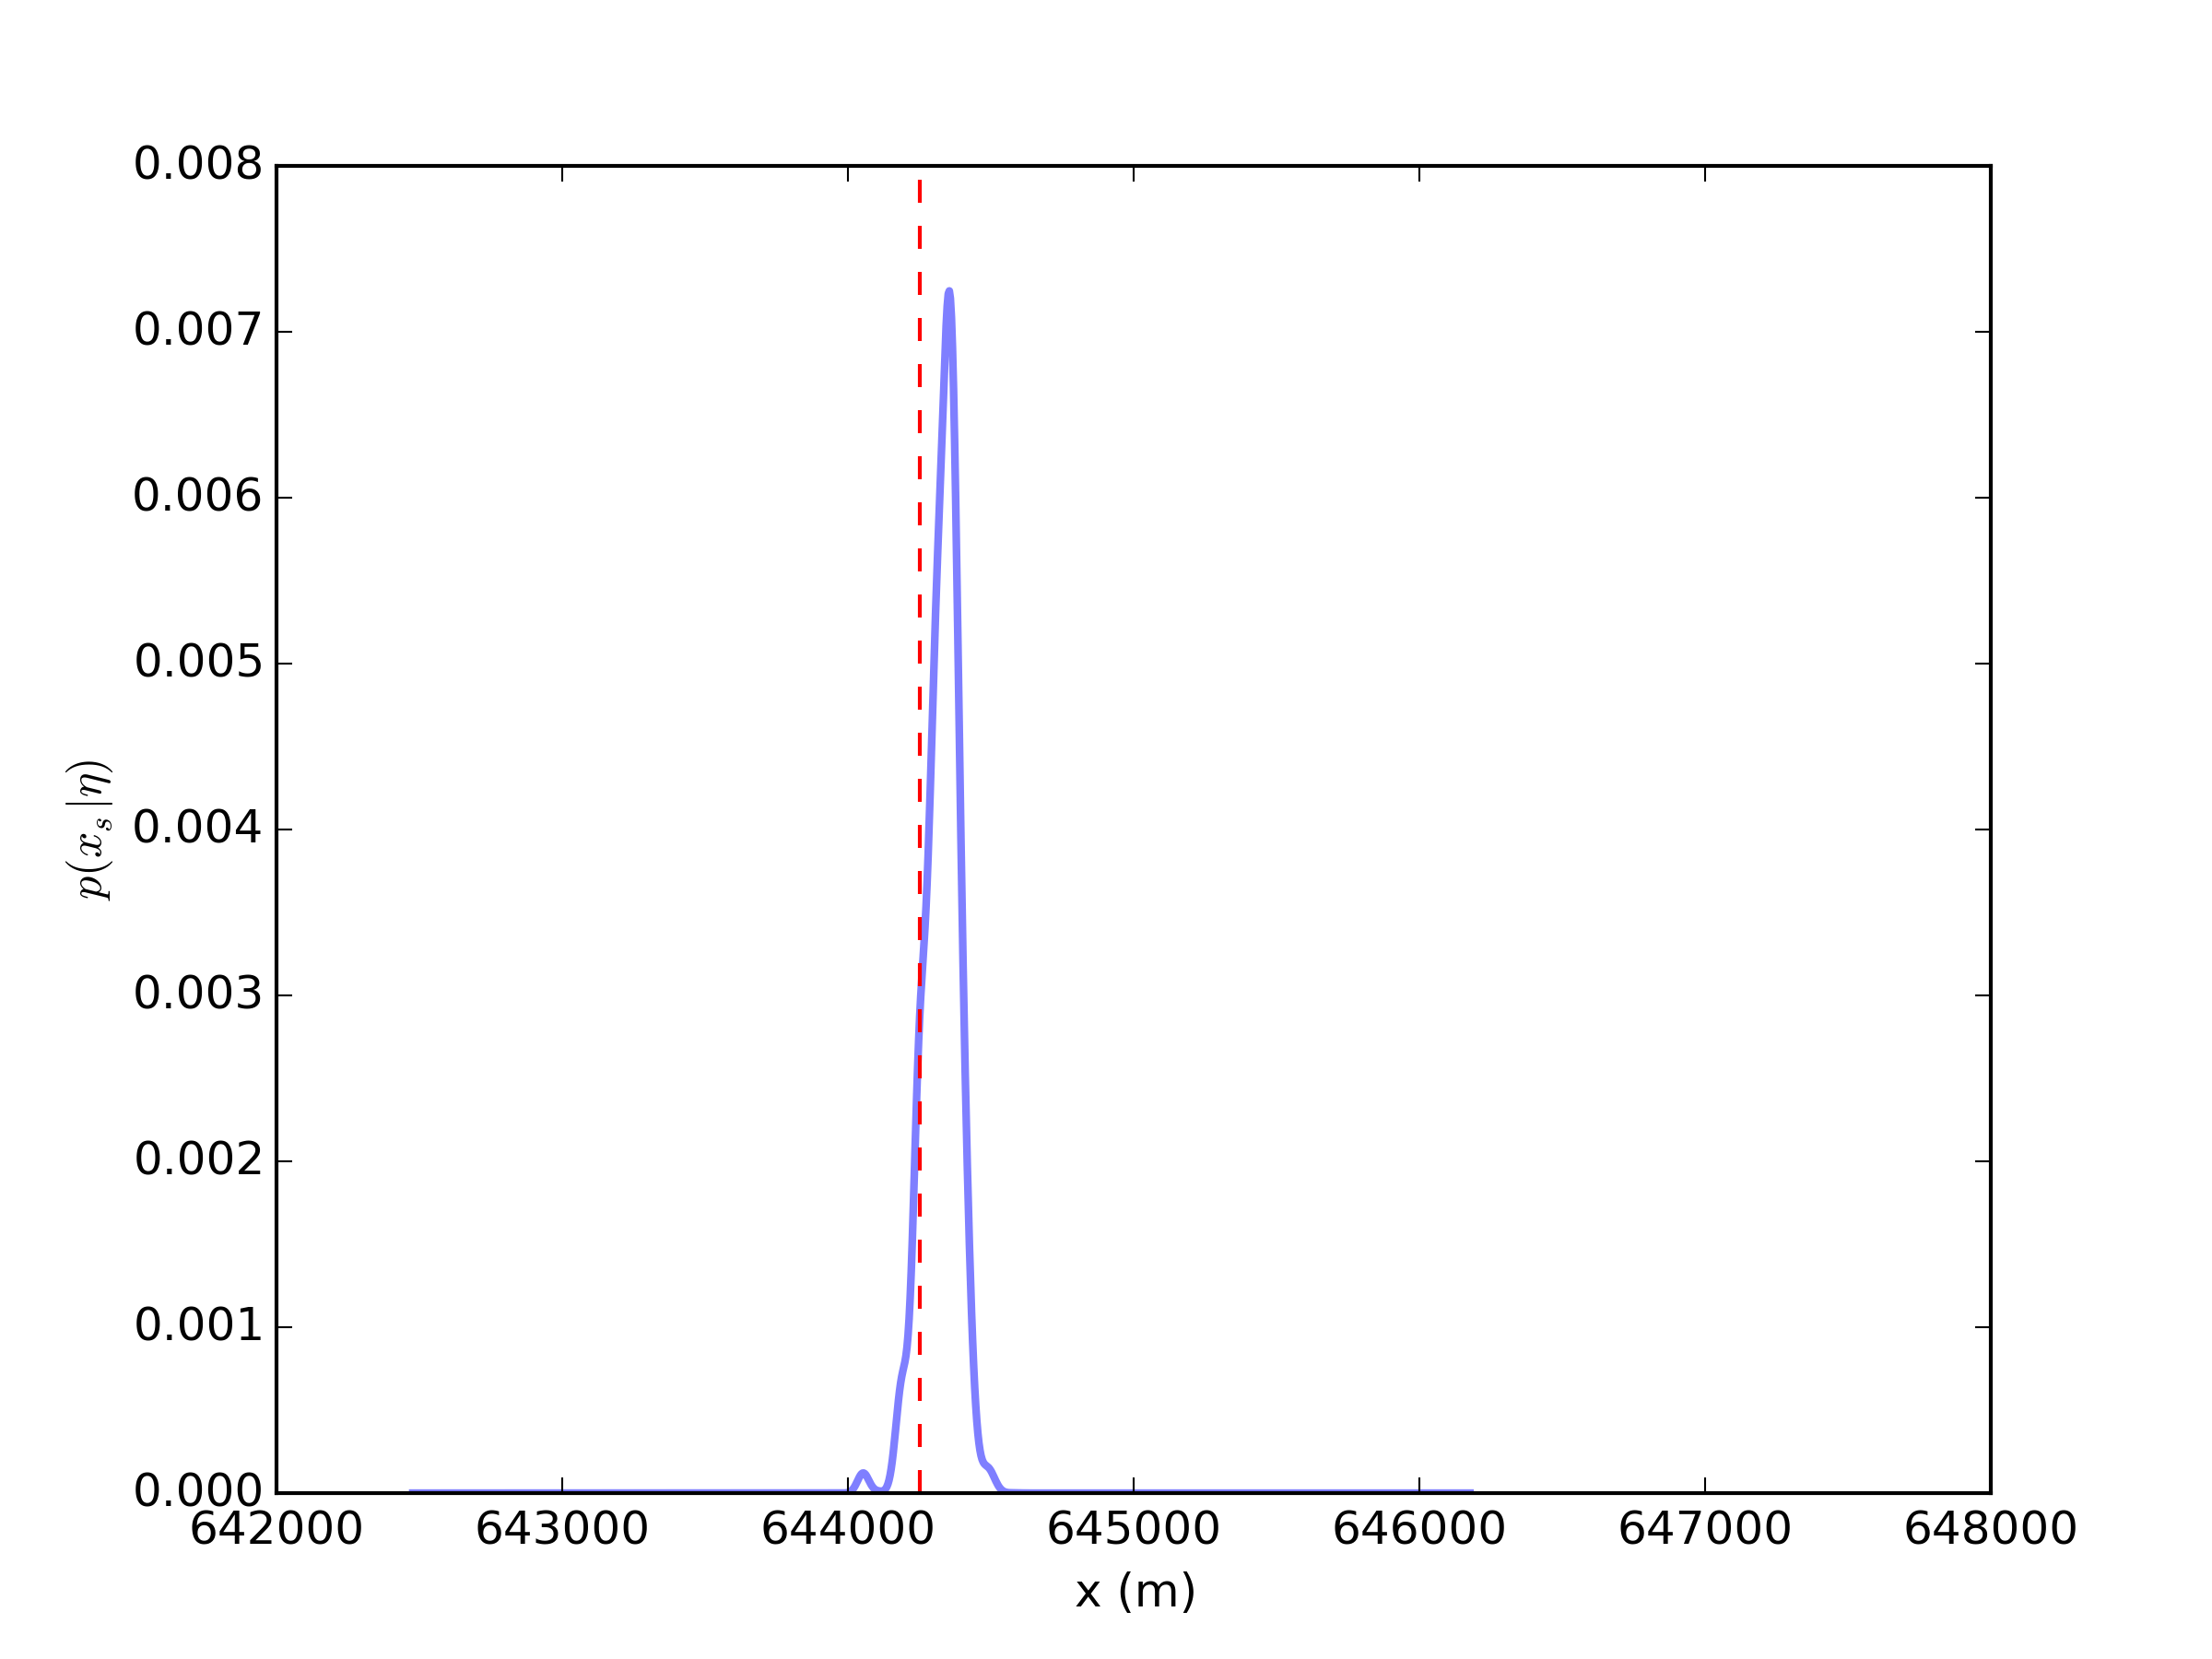
\includegraphics[width=1\textwidth]{25C_prelim_X.png}
 		\caption{Position en $x$}
 		\label{fig_25C_prelim_X}
 	\end{subfigure}%
 	\begin{subfigure}[t]{0.5\textwidth}
 		\centering
 		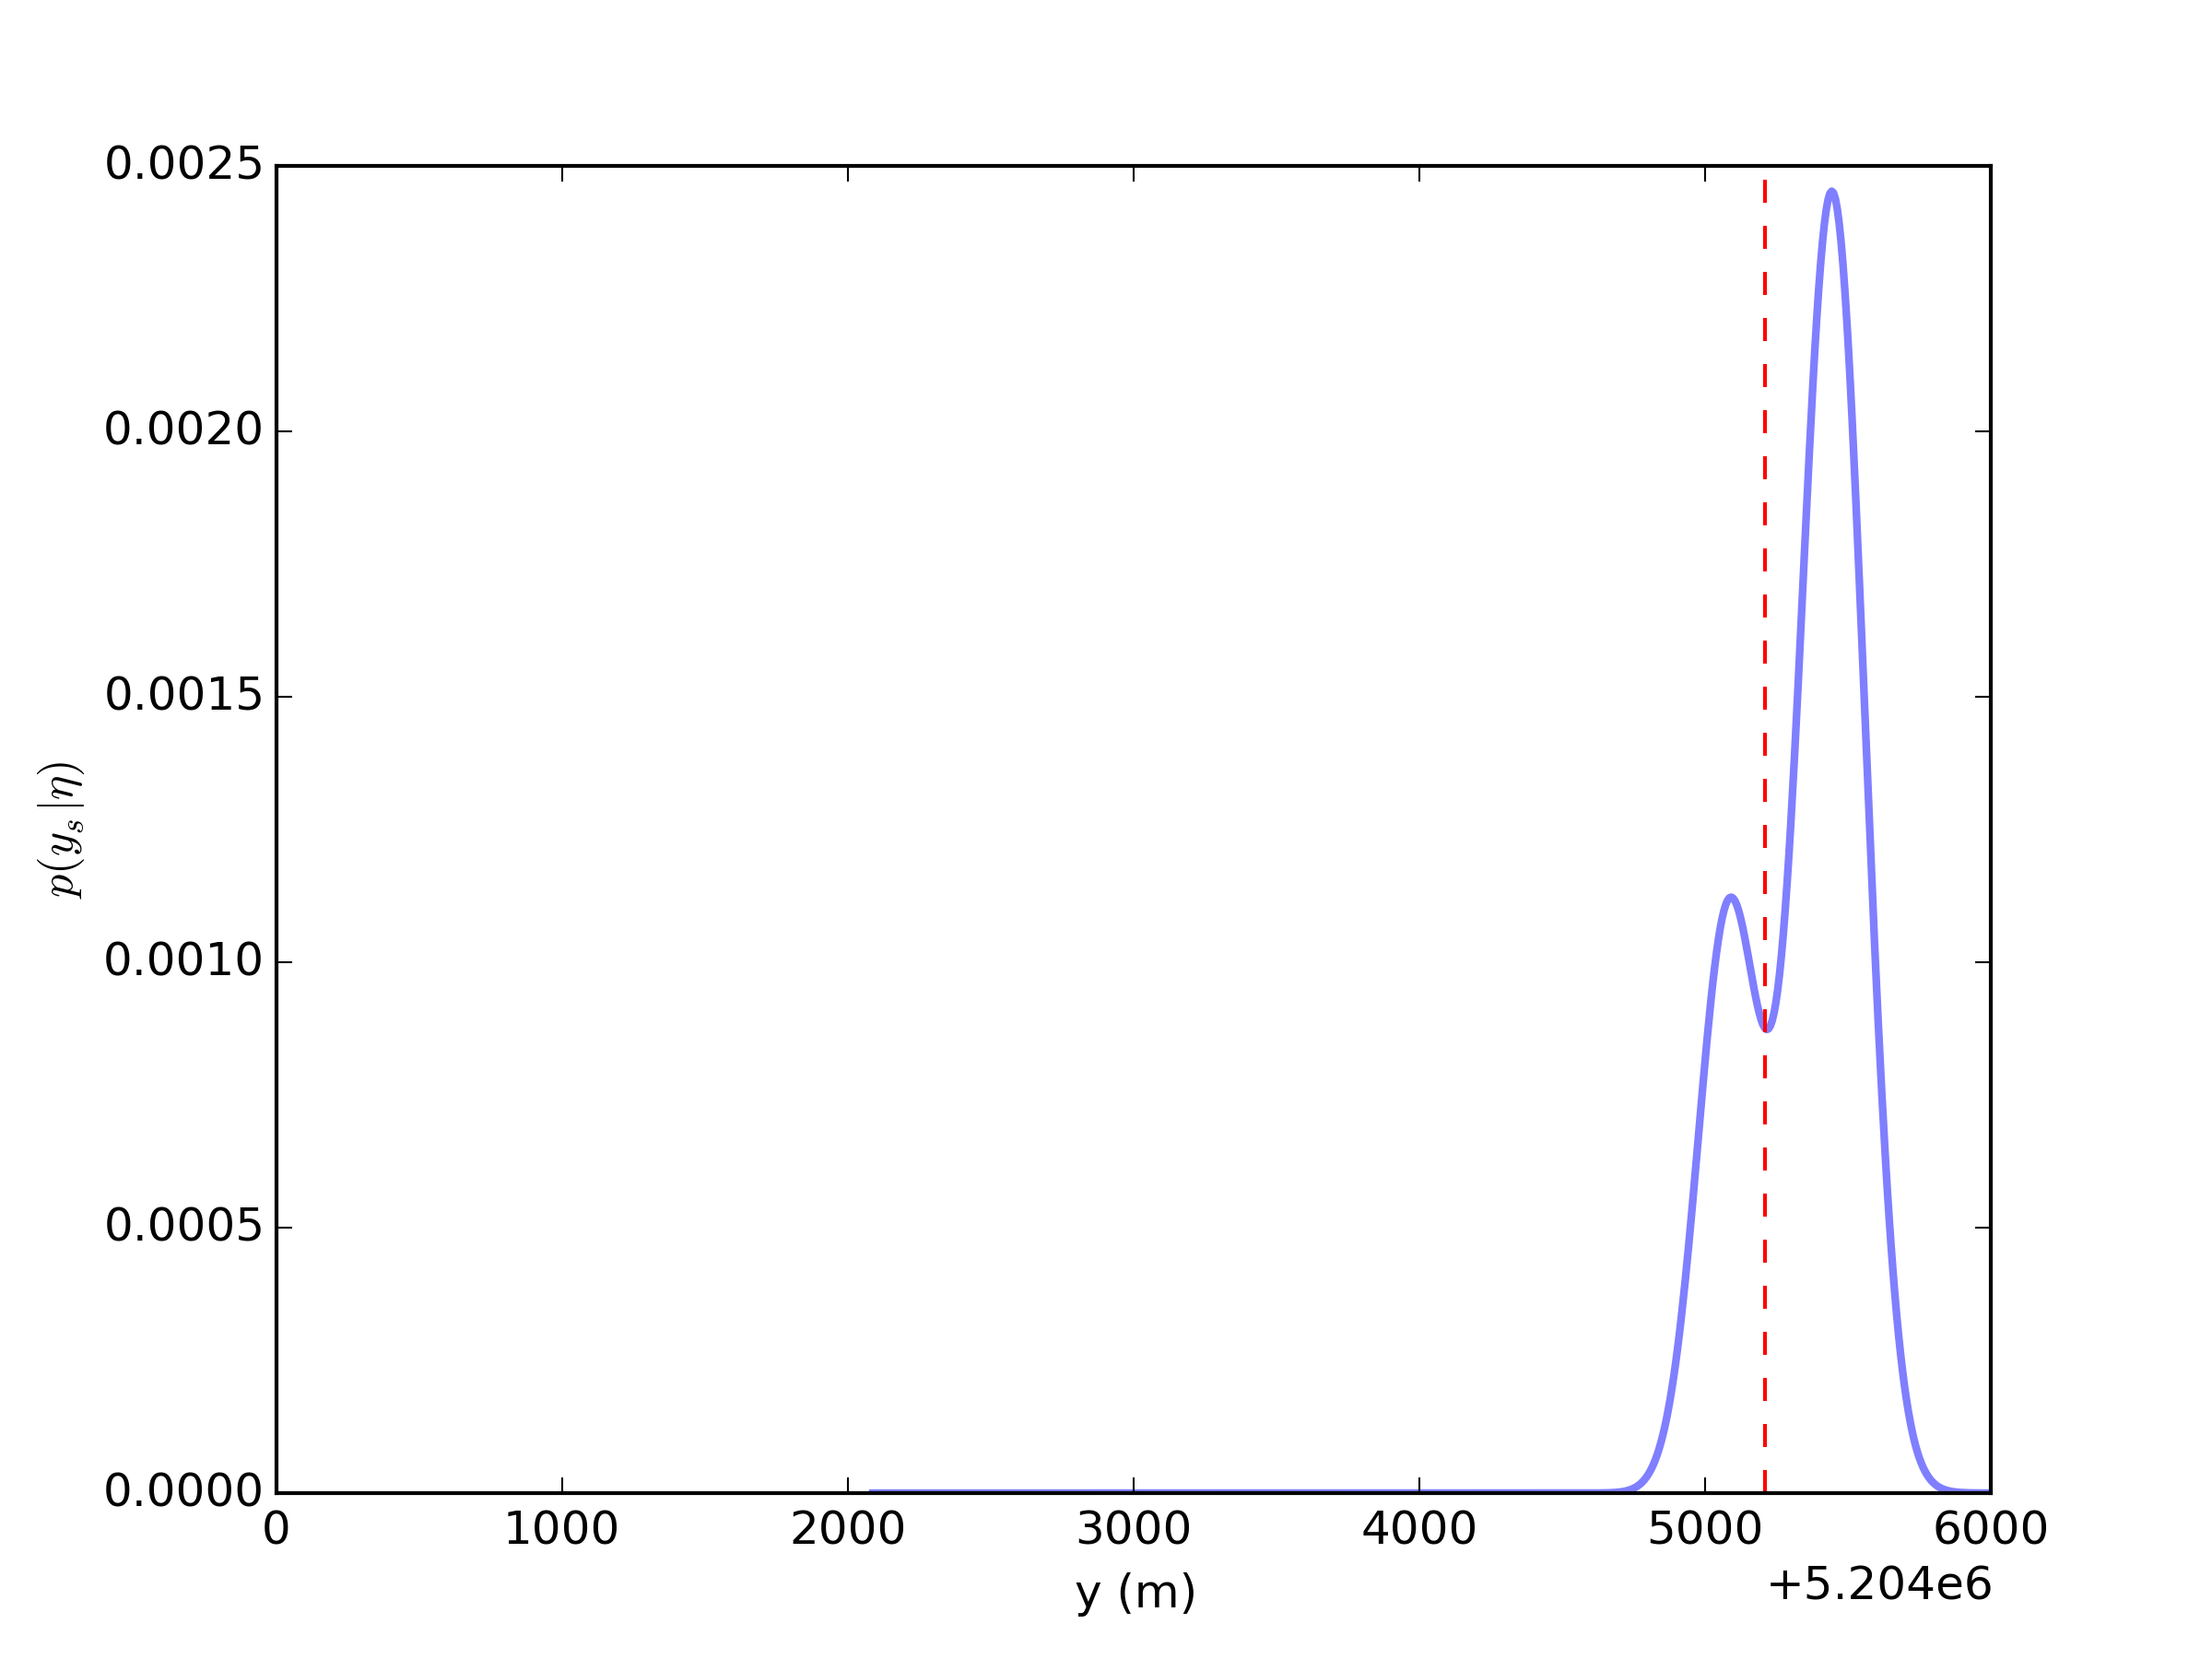
\includegraphics[width=1\textwidth]{25C_prelim_Y.png}
 		\caption{Position en $y$}
 		\label{fig_25C_prelim_Y}
 	\end{subfigure}
 	\begin{subfigure}[t]{0.65\textwidth}
 		\centering
 		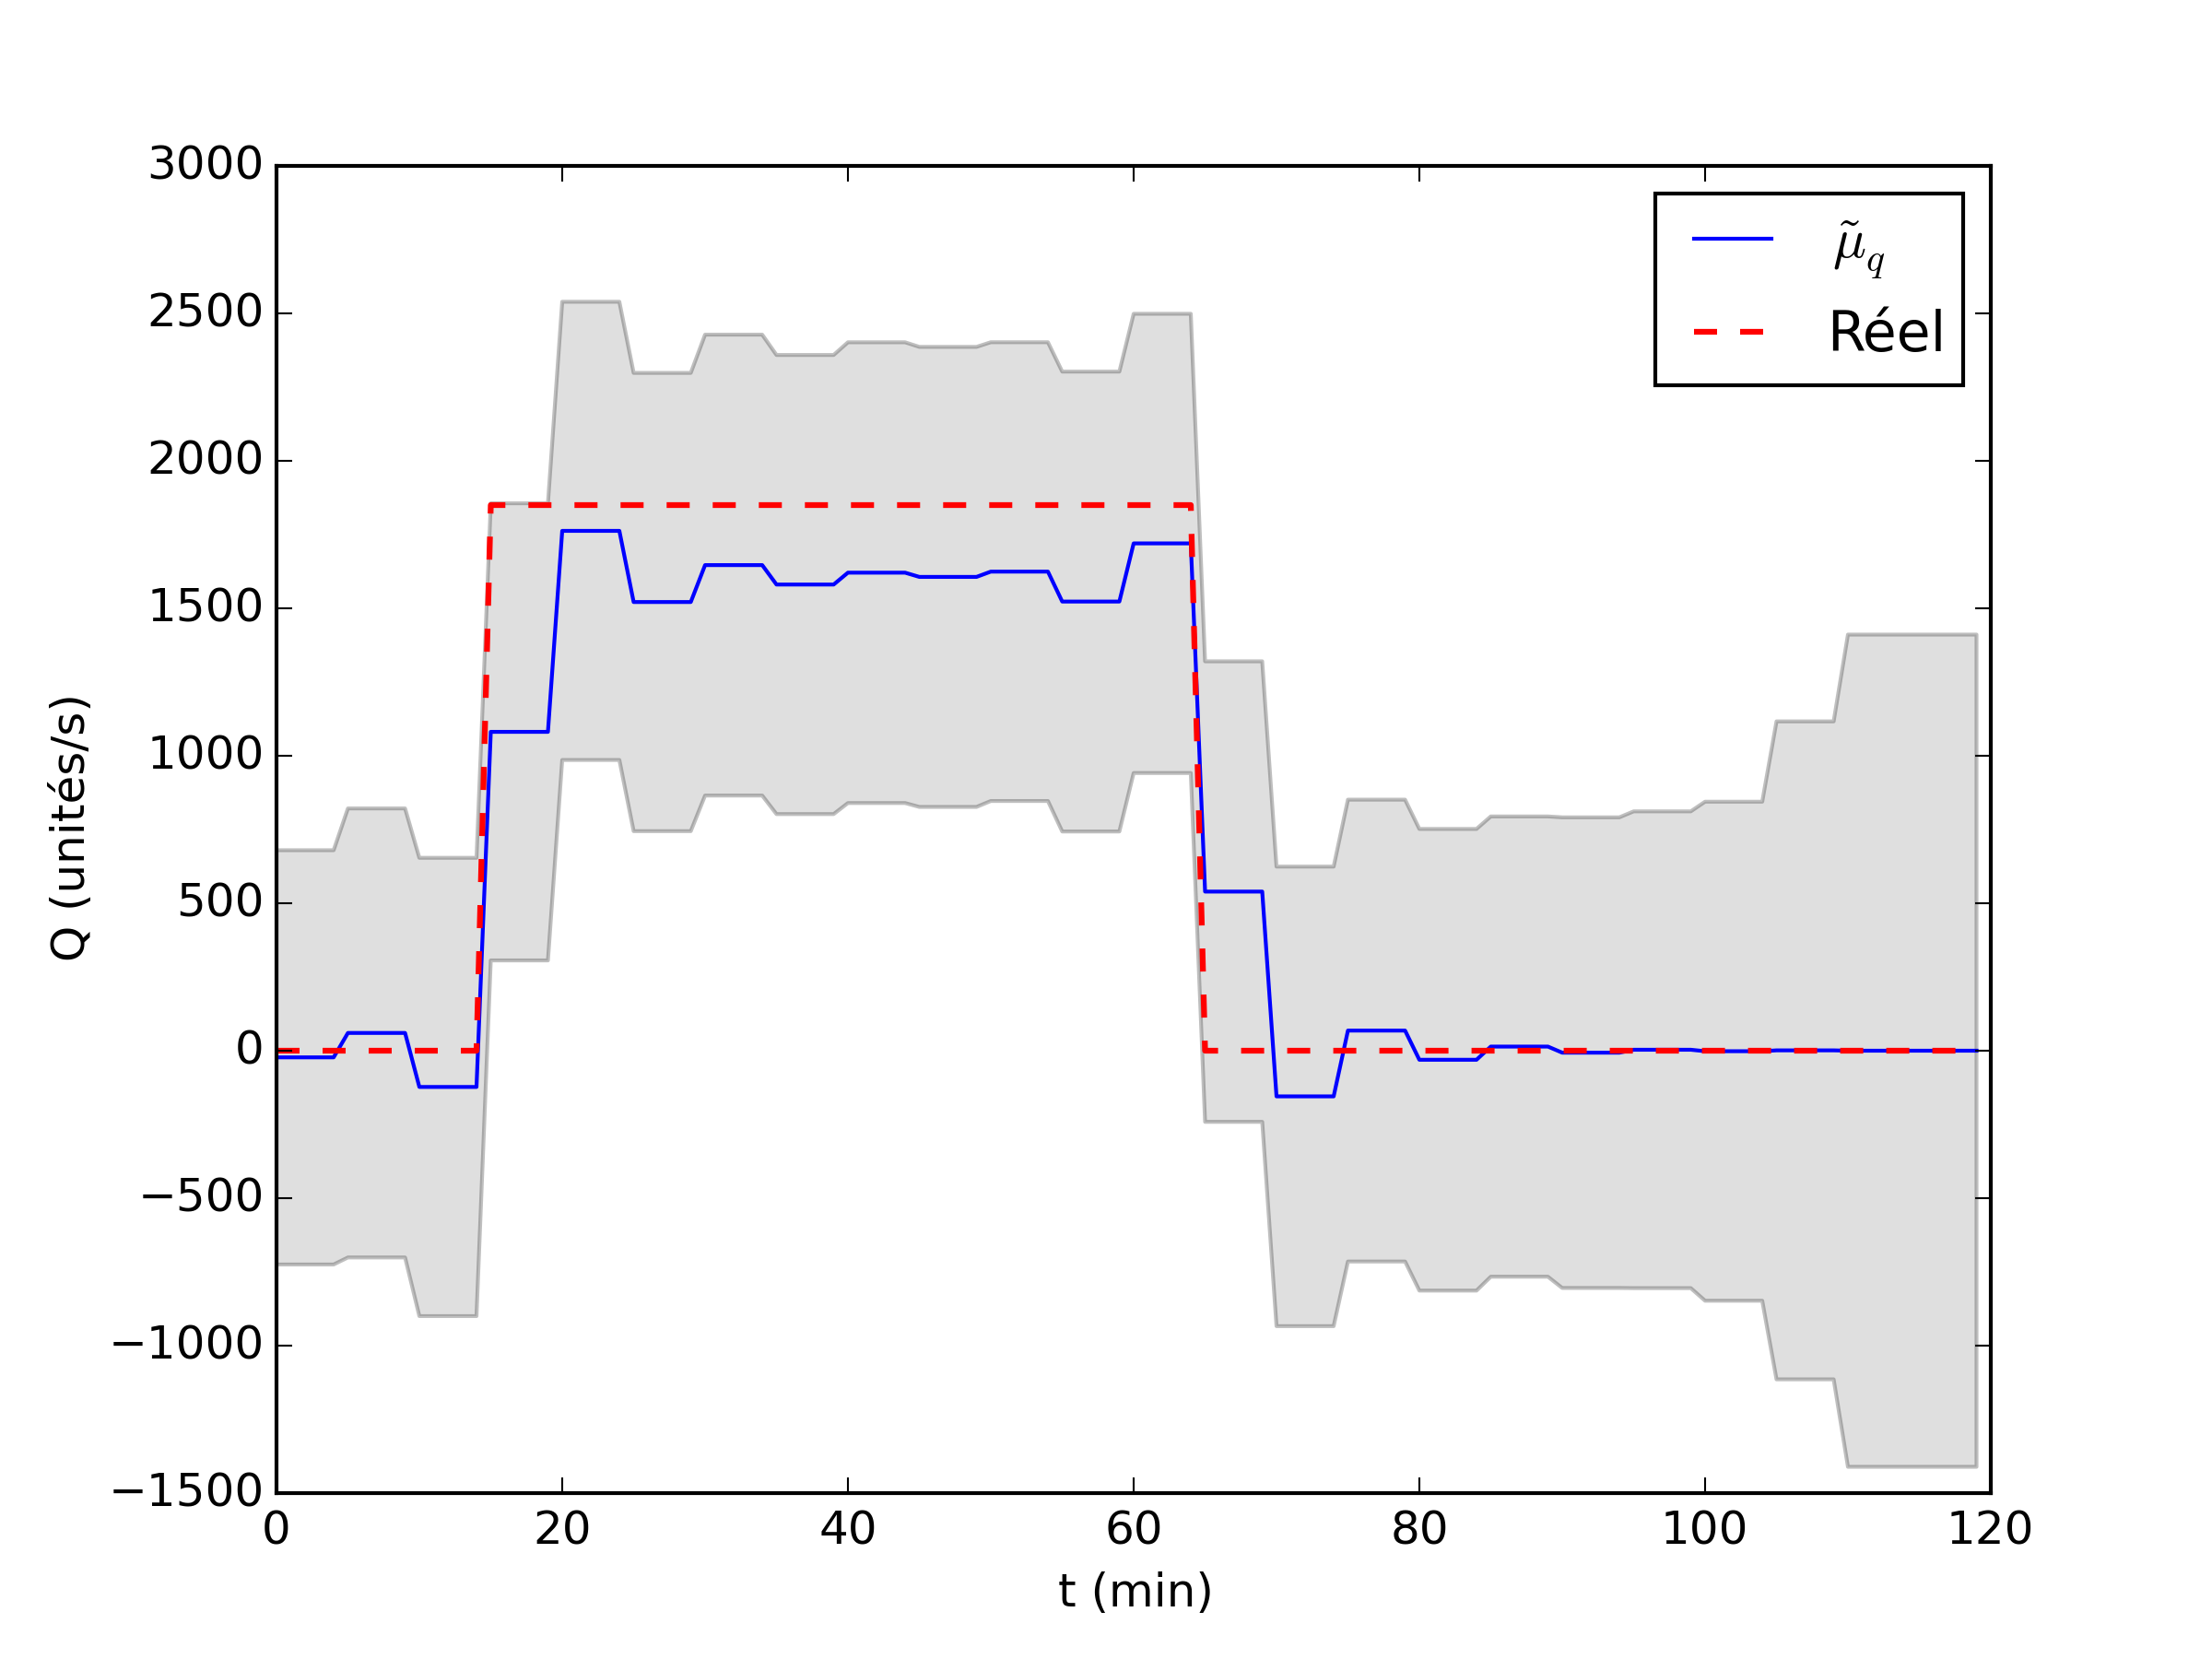
\includegraphics[width=1\textwidth]{25C_prelim_Q.png}
 		\caption{Profil d'émission avec intervalle de confiance à  $\pm 2 \widetilde{\sigma}_q^2$ (gris)}
 		\label{fig_25C_prelim_Q}
 	\end{subfigure} 
 	\caption{Résultats du \textit{benchmark} de l'algorithme d'estimation sur le cas-test Beaune}
 	\label{fig_25C_prelim}
 \end{figure}
 
 Pour mesurer l'erreur relative d'une estimation ponctuelle par rapport à la vraie position de la source, on utilise la métrique suivante:
 
 \begin{equation}
	 r_d = \dfrac{d(\Vecx_s,\widehat{\Vecx}_{MMSE})}{L_{\mathcal{D}}}
 \end{equation}
 où:
 \begin{itemize}
 	\item $L_{\mathcal{D}}$ est la diagonale du domaine $\mathcal{D}$ considéré, autrement dit la plus grande distance possible entre deux points: cela permet de borner $r_d$ entre 0 et 1,
 	\item $\Vecx_s$ est le centre de la maille où est située la source,
 	\item $\widehat{\Vecx} _{MMSE}$ est l'estimation ponctuelle par MMSE de la position de la source obtenue via les particules et les poids d'importance fournis en sortie de l'AMIS.
 \end{itemize}
 
 Pour mesurer l'erreur d'estimation du débit, on utilise l'erreur quadratique moyenne définie par:
 \begin{equation}
	 Err(\tilde{\VecMeanQ}) = \dfrac{1}{T_s} \sum\limits_{i=1}^{T_s}(\VecQSource^{(i)} - \tilde{\VecMeanQ}^{(i)})^2
 \end{equation}
 où $\VecQSource$ est le profil d'émission réel et $\tilde{\VecMeanQ}$ est le profil estimé.\\
 
 Dans l'exemple de la figure \ref{fig_25C_prelim}, on obtient ainsi une erreur relative de $r_d = 0.017$ pour la position, et une erreur d'estimation du débit de $Err(\tilde{\VecMeanQ}) = 296.909$. \\
 
 Nous étudions dans les paragraphes suivants l'influence des paramètres de variance d'observation $\varObs$ et de variance a priori $\varQ$ du profil d'émission $\VecQSource$ sur la qualité de l'estimation. Une telle étude paramétrique permet en effet de donner du sens à ces paramètres, ceux-ci devant être spécifiés par l'utilisateur parmi les variables d'entrée de l'algorithme d'estimation. 
 
 \subsection{Influence de la variance d'observation}
 
 La variance d'observation $\varObs$ est le paramètre qui reflète la "confiance" donnée aux observations $\VecObs$. Comme expliqué au Chapitre 3, elle caractérise l'ensemble des erreurs à l'origine de l'écart entre les valeurs issues du modèle de données et la réalité physique. Comme il a été expliqué précédemment, l'erreur d'observation est une agrégation de diverses sources individuelles d'erreur (modèle, instrumentation...). Sans chercher à mener une analyse approfondie sur la quantification des incertitudes autour des observations, nous cherchons plutôt ici à avoir une vision d'ensemble de l'influence du paramètre $\varObs$ sur la qualité de l'estimation du terme source. Pour cela, on garde les mêmes paramètres que le \textit{benchmark} de la figure \ref{fig_25C_prelim}, on choisit ensuite une plage de valeurs de $\varObs$ à tester, et pour chacune de ces valeurs, on lance 100 \textit{runs} de l'AMIS. Ce dernier faisant intervenir des tirages aléatoires, le fait de considérer les résultats issus d'un nombre suffisant de \textit{runs} permet de voir si la qualité des estimations n'est pas perturbée par ces aspects stochastiques. Les valeurs de variance choisies sont $10^{-7}, 5\times 10^{-7}, 10^{-6}, 5\times 10^{-6}, 10^{-5}, 5\times 10^{-5},10^{-4}$. \\
   
         Concernant la localisation de la source, on observe sur les figures \ref{fig_25C_analyse_varobs_x} et \ref{fig_25C_analyse_varobs_y} de l'Annexe A que les résultats sont plutôt réguliers: l'estimation de la position est bonne pour les valeurs inférieures à $5\times 10^{-6}$ puis se dégrade progressivement jusqu'à avoir du mal à définir une zone précise de l'espace (\ref{varF_x} et \ref{varF_y}).
         
         Pour le profil d'estimation sur la figure \ref{fig_25C_analyse_varobs_q} de l'Annexe A, celui-ci est relativement bien estimé pour $\varObs=10^{-7}$, les variations étant de plus en plus importantes au fur et à mesure que la valeur de la variance d'observation augmente. Les courbes d'erreur de la figure \ref{fig_25C_varobs_erreurs} donnent un aperçu de l'influence générale de la variance d'observation.
         
         \begin{figure}[h!]
         	\centering
         	\includegraphics[width=0.8\textwidth]{25C_varobs_errors.png}
         	\caption{Courbes d'erreur pour l'analyse paramétrique de $\varObs$}
         	\label{fig_25C_varobs_erreurs}
         \end{figure}
         
         
         Certaines des valeurs estimées pour le débit soient négatives, or il a été constaté que l'application de la contrainte de positivité a tendance à surestimer les valeurs de $\tilde{\VecMeanQ}$, comme le montre l'exemple de la figure \ref{fig_sansavecPC}. Il a donc été décidé de ne pas implémenter cette contrainte, car malgré la présence de quelques valeurs négatives, le sens physique des résultats d'estimation est globalement respecté.
       
\begin{figure}[h!]
    	\centering
         	\begin{subfigure}[t]{0.5\textwidth}
         		\centering
         		\includegraphics[width=1\textwidth]{1part_sansPC.png}
         		\caption{}
         		\label{sansPC}
         	\end{subfigure}%
         	\begin{subfigure}[t]{0.5\textwidth}
         		\centering
         		\includegraphics[width=1\textwidth]{1part_avecPC.png}
         		\caption{}
         		\label{avecPC}
         	\end{subfigure}
         	\caption{Comparaison de l'estimation de $\tilde{\VecMeanQ}$ sur une particule dans la maille de la source sans (à gauche) et avec (à droite) la contrainte de positivité}
         	\label{fig_sansavecPC}
         \end{figure}

En examinant les résultats des figures précédentes, on pourrait considérer la valeur $\varObs = 10^{-7}$ comme étant celle qui donne les meilleurs résultats. Il faut cependant rappeler que dans notre cas d'étude, nous utilisons des observations synthétiques non-bruitées, ce qui permet d'accorder une plus grande confiance à ces observations et donc de réduire la valeur de $\varObs$. On ne peut pas forcément en faire autant si des sources d'incertitudes supplémentaires entrent en jeu, par exemple avec des valeurs de concentrations expérimentales issues de mesures réelles, car cela reviendrait à diminuer la marge d'incertitude sur les mesures alors que le caractère aléatoire de ces dernières est plus accentué. 
%
%Pour illustrer le rôle de l'incertitude des mesures dans le choix du paramètre $\varObs$, on perturbe le vecteur d'observation $\VecObs$ avec un bruit additif gaussien centré, et pour préserver la cohérence physique de la simulation, on ramène les observations bruitées négatives à 0. L'intensité de la perturbation du signal d'observation est ainsi caractérisée par la variance du bruit $\varBruit$ choisie: on considère ici 3 différents niveaux dont l'impact sur $\VecObs$ est illustré par la figure \ref{fig_25_obs_noisy}.\\
%\begin{figure}[h!]
%	\centering
%	\begin{subfigure}[t]{0.33\textwidth}
%		\centering
%		\includegraphics[width=1\textwidth]{25C_obs_noisy_1E4.png}
%		\caption{}
%		\label{}
%	\end{subfigure}%
%	\begin{subfigure}[t]{0.33\textwidth}
%		\centering
%		\includegraphics[width=1\textwidth]{25C_obs_noisy_5E4.png}
%		\caption{}
%		\label{}
%	\end{subfigure}%
%	\begin{subfigure}[t]{0.33\textwidth}
%		\centering
%		\includegraphics[width=1\textwidth]{25C_obs_noisy_1E3.png}
%		\caption{}
%		\label{}
%	\end{subfigure}%
%	\caption{Perturbation du vecteur d'observations $\VecObs$ par différentes intensités de bruit}
%	\label{fig_25C_obs_noisy}
%\end{figure}
%
%On  étudie ensuite les résultats d'estimation obtenus avec chacun de ces nouveaux vecteurs d'observations pour une variance $\varObs = 10^{-7}$ afin de comparer les différences de résultats avec et sans ajout de bruit.\\
%
%\todoin{1) Comparaison avec et sans bruit 2) Conclusion}

\subsection{Influence de la variance a priori du profil d'émission}

La variance a priori $\varQ$ peut être vue comme une hypothèse de départ sur l'amplitude possible des valeurs du profil d'émission. Son influence s'applique à la fois sur la qualité de la reconstruction de $\VecQSource$, mais également sur celle de la localisation de la source, car $\varQ$ intervient dans l'algorithme AMIS lors du calcul de la vraisemblance des particules. 

Pour cette analyse, on utilise le même procédé que pour l'étude de $\varObs$, en reprenant les paramètres du \textit{benchmark} et en exécutant 100 \textit{runs} de l'AMIS, les valeurs de $\varQ$ couvertes étant: $2\times 10^5, 7\times 10^5, 2\times 10^6, 7\times 10^6, 2\times 10^7$ et $7\times 10^7$.\\

Pour l'estimation de la position, on constate que plus la valeur de $\varQ$ considérée est grande, plus la source aura tendance à être estimée en amont  par rapport à la direction du vent. En effet, pour la même position potentielle de la source, des valeurs plus élevées pour les quantités de polluant rejetées impliquent des mesures de concentration plus importantes aux capteurs: l'algorithme va donc ajuster cette position en remontant l'axe du vent pour avoir une meilleure vraisemblance par rapport aux observations. Ce phénomène de décalage spatial est bien visible sur la figure \ref{fig_25C_varQ_boxplots}, où les \textit{boxplots} des estimations ponctuelles sont tracées pour chacune des valeurs de $\varQ$ testées.

\begin{figure}[h!]
	\centering
         	\begin{subfigure}[t]{0.5\textwidth}
         		\centering
         		\includegraphics[width=1\textwidth]{25C_varQ_boxplot_x.png}
         		\caption{}
         		\label{varQ_boxplot_x}
         	\end{subfigure}%         	
         \begin{subfigure}[t]{0.5\textwidth}
         	\centering
         	\includegraphics[width=1\textwidth]{25C_varQ_boxplot_y.png}
         	\caption{}
         	\label{varQ_boxplot_y}
         \end{subfigure}%
         \caption{\textit{Boxplots} des estimations par MMSE de la position de la source sur 100 runs, comparaison avec les valeurs réelles (en pointillés noirs)}
         \label{fig_25C_varQ_boxplots}
	
\end{figure}

La meilleure estimation du profil d'émission est obtenue pour $\varQ=2\times 10^6$ (voir figure \ref{fig_25C_analyse_varq_q} de l'Annexe A), ce qui coïncide avec la meilleure position estimée dans la figure \ref{fig_25C_varQ_boxplots}. Pour des valeurs plus faibles de $\varQ$ le débit est sous-estimé, à l'inverse pour des valeurs plus élevées le débit est surestimé. On peut résumer ce comportement grâce aux courbes d'erreur de la figure \ref{fig_25C_varq_erreurs}.

         \begin{figure}[h!]
         	\centering
         	\includegraphics[width=0.8\textwidth]{25C_varQ_errors.png}
         	\caption{Courbes d'erreur pour l'analyse paramétrique de $\varQ$}
         	\label{fig_25C_varq_erreurs}
         \end{figure}

\subsection{Influence de la densité du réseau de capteurs}

Le nombre et de la répartition des capteurs constitue un facteur important: 

\begin{itemize}
	\item du point de vue théorique, son étude permet de mieux comprendre le comportement de l'algorithme d'estimation et quantifier son importance par rapport aux autres variables,
	\item en pratique, l'analyse des résultats d'estimation en fonction de la configuration des capteurs permet un meilleur dimensionnement du réseau de mesure.\\
\end{itemize}

\subsubsection{Impact du capteur R8}

Dans un premier temps, nous nous intéressons à l'influence du capteur R8, qui est le récepteur le plus proche de la source à mesurer des concentrations non-nulles. Pour cela, nous le retirons du réseau, et nous effectuons l'opération d'estimation du terme source avec les observations issues des 24 capteurs restants, en suivant les paramètres du \textit{benchmark}. En pratique, cela reviendrait par exemple à simuler la panne du capteur R8 durant la fenêtre temporelle d'observation.\\


\begin{figure}[h!]
	\centering
	\begin{subfigure}[t]{0.5\textwidth}
		\centering
		\includegraphics[width=1\textwidth]{R8_kde_x_compare.png}
		\caption{Position en $x$}
		\label{R8_x}
	\end{subfigure}%
	\begin{subfigure}[t]{0.5\textwidth}
		\centering
		\includegraphics[width=1\textwidth]{R8_kde_y_compare.png}
		\caption{Position en $y$}
		\label{R8_y}
	\end{subfigure}
	\begin{subfigure}[t]{0.65\textwidth}
		\centering
		\includegraphics[width=1\textwidth]{R8_q_est_compare.png}
		\caption{Profil d'émission avec intervalle de confiance à  $\pm 2 \tilde{\sigma}_q^2$}
		\label{R8_q}
	\end{subfigure} 
	\caption{Résultats d'un \textit{run} de l'algorithme d'estimation sans (jaune) et avec (bleu) le capteur R8}
	\label{fig_R8_compare}
\end{figure}

A paramètres identiques, la source est vue plus en amont sur l'axe du vent par rapport à sa position réelle (figures \ref{R8_x} et \ref{R8_y}). De plus, sans le capteur R8, le débit est relativement sous-estimé par rapport aux valeurs attendues, et le rejet reconstitué commence et s'achève plus tôt que prévu (figure \ref{R8_q}). On observe ainsi que les mesures fournies par le capteur R8 apportent une information non-négligeable permettant d'accroître la précision de l'estimation, à la fois sur les aspects spatiaux, temporels, et de quantité émise. 

\subsubsection{Impact d'un réseau réduit}

On a vu que le rôle individuel des capteurs peut être important pour pouvoir reconstruire correctement un terme source. Nous cherchons ici à savoir comment varie la qualité de cette reconstruction si l'ensemble du réseau est modifié.

On réduit ainsi la taille de notre réseau à 9 capteurs (figure \ref{fig_reseaux_25_9}), répartis de façon homogène sur le domaine. Cela permet de simuler une situation où le nombre d'instruments de mesure des concentrations est moindre (par exemple, dans le cas où les capteurs sont coûteux à acheter et à déployer), et également d'apprécier le comportement de l'algorithme d'estimation lorsque la représentativité spatiale des mesures est limitée. Les paramètres d'entrée de l'algorithme d'estimation sont toujours ceux du \textit{benchmark}.\\

\begin{figure}[h!]
	\centering
	\begin{subfigure}[t]{0.5\textwidth}
		\centering
		\includegraphics[width=1\textwidth]{reseau_25C.png}
		\caption{}
		\label{reseau_25C}
	\end{subfigure}%
	\begin{subfigure}[t]{0.5\textwidth}
		\centering
		\includegraphics[width=1\textwidth]{reseau_9C.png}
		\caption{}
		\label{reseau_9C}
	\end{subfigure}
	\caption{Réduction de la densité du réseau de capteurs: passage de 25 (gauche) à 9 (droite) capteurs}
	\label{fig_reseaux_25_9}
\end{figure}


\begin{figure}[h!]
	\centering
	\begin{subfigure}[t]{0.5\textwidth}
		\centering
		\includegraphics[width=1\textwidth]{kde_x_compare_all.png}
		\caption{}
		\label{kde_x_all}
	\end{subfigure}%
	\begin{subfigure}[t]{0.5\textwidth}
		\centering
		\includegraphics[width=1\textwidth]{kde_y_compare_all.png}
		\caption{}
		\label{kde_y_all}
	\end{subfigure}
	\begin{subfigure}[t]{0.33\textwidth}
		\centering
		\includegraphics[width=1\textwidth]{q_9C.png}
		\caption{}
		\label{q_9C}
	\end{subfigure}%
	\begin{subfigure}[t]{0.33\textwidth}
		\centering
		\includegraphics[width=1\textwidth]{q_24C.png}
		\caption{}
		\label{q_24C}
	\end{subfigure}%
	\begin{subfigure}[t]{0.33\textwidth}
		\centering
		\includegraphics[width=1\textwidth]{q_25C.png}
		\caption{}
		\label{q_25C}
	\end{subfigure}
	\caption{Résultats d'un \textit{run} de l'algorithme d'estimation sans (jaune) et avec (bleu) le capteur R8, comparaison avec un réseau réduit (vert)}
	\label{}
\end{figure}



Les résultats de  localisation de la source montrent une dégradation de l'estimation de la position similaire au cas où le capteur R8 n'est pas présent (figures \ref{kde_x_all} et \ref{kde_y_all}). Il en va de même pour pour l'estimation du profil de rejet (figures \ref{q_9C}, \ref{q_24C} et \ref{q_25C}), où la marge d'incertitude est même légèrement moins grande dans la configuration à capteurs. 

On peut ainsi en déduire que les capteurs n'observant aucune concentration  non-nulle et qui ont été retirés pour établir la configuration à 9 capteurs ont bien un rôle informatif utile au processus d'estimation, et leur apport qualitatif par rapport à la présence du capteur R8 dans le réseau à 25 capteurs semble de même importance.\\

De façon générale, on peut ainsi voir que l'efficacité de l'estimation du terme source repose sur un certain nombre de paramètres d'entrée pour l'algorithme AMIS. Ceux-ci peuvent dépendre entièrement de la configuration du cas-test (nombre de capteur et disposition sur le domaine), ou être définis manuellement par l'utilisateur. Dans ce dernier cas, on a constaté qu'il est difficile d'établir des critères empiriques pour choisir des valeurs par défaut à affecter aux paramètres de variance $\varObs$ et $\varQ$. Pour la variance d'observation, un choix qualitatif a été fait par rapport à l'allure des mesures de la figure \ref{fig_observations_25CAPTEURS}, mais dans d'autres situations pratiques, l'évaluation de $\varObs$ peut se révéler plus compliquée:
\begin{itemize}
	\item si on sait d'avance que certains capteurs du réseau sont plus fiables que d'autres et qu'on choisit d'accorder une plus grande confiance à ces capteurs, alors l'hypothèse d'une loi d'incertitude identiquement distribuée sur les éléments du vecteur d'observation n'est plus valable,
	\item dans un cas opérationnel où on aurait choisi une variance d'observation trop faible, le biais par rapport à la position réelle de la source peut se révéler suffisamment important pour que cette dernière ne soit pas incluse dans l'intervalle de confiance accordé à l'estimation.
\end{itemize}

Pour la variance a priori $\varQ$, le problème est similaire à celui du choix de la matrice d'erreur de \textit{background} en assimilation de données, où la qualité de l'ébauche du terme source fournie influe directement sur la qualité de la reconstruction. 

Une alternative plausible à cette recherche difficile des paramètres initiaux consisterait à travailler sur un ensemble de scénarios possibles, et ainsi d'étudier plusieurs possibilités quant aux valeurs des variances à fournir. Cela demeure possible grâce au gain d'efficacité de calcul permis par l'approche \textit{backward} de l'AMIS, et permettrait d'envisager différents niveaux de confiance accordés aux observation (pour $\varObs$), ainsi que plusieurs hypothèses sur le profil du rejet (pour $\varQ$). Le résultat serait alors un ensemble d'estimations  sur les termes sources possibles selon ces valeurs d'entrée, dont la pertinence serait alors évaluée par les décideurs et les experts en fonction de leur expérience et de la réalité du terrain.




 
 
 





	
	\bibliographystyle{apalike}
	\bibliography{_biblio}
\end{document}

